\documentclass{article}
\usepackage[utf8]{inputenc}
\usepackage[english]{babel}
\usepackage[margin=0.8in]{geometry} % Page Dimensions
\usepackage{tgschola}

\usepackage{cancel}
\usepackage{enumitem}
\setlength{\parskip}{\baselineskip}%
\usepackage[breakable,many]{tcolorbox}
% Math
\usepackage{amsmath, amsthm, amssymb}
\usepackage[inline]{asymptote}
\usepackage{xcolor}

% Allows for hyperlinking
\usepackage{hyperref}
\hypersetup{
    colorlinks=true,
    linkcolor=magenta,
}

%%%%%%%%%%%%%%%%%%%%%%%%%%%%%%%%%%%%%%%%%%%%%%%%%%%%%%%%%%
%%%%%%%%%%%%%%%%%%%%%%% COLORS %%%%%%%%%%%%%%%%%%%%%%%%%%%
%%%%%%%%%%%%%%%%%%%%%%%%%%%%%%%%%%%%%%%%%%%%%%%%%%%%%%%%%%

\definecolor{my-blue}{RGB}{93,169,233}
\definecolor{my-pink}{RGB}{238,118,116}
\definecolor{my-green}{RGB}{0,191,0}
\definecolor{my-orange}{HTML}{C78058}
\definecolor{background}{HTML}{f2f2f2}
\definecolor{my-yellow}{HTML}{F6BD60}

%%%%%%%%%%%%%%%%%%%%%%%%%%%%%%%%%%%%%%%%%%%%%%%%%%%%%%%%%%
%%%%%%%%%%%%%%%%%% Style Definitions %%%%%%%%%%%%%%%%%%%%%
%%%%%%%%%%%%%%%%%%%%%%%%%%%%%%%%%%%%%%%%%%%%%%%%%%%%%%%%%%

\tcbset{simple/.style={
    breakable,
    enhanced,
    outer arc=0pt,
    arc = 0pt,
    colback=background, % Background color
    colframe=background, % Border Color
    coltitle=black, % Title Color
    fonttitle=\bfseries,
    attach title to upper,
    after title={:\ },
    segmentation style={dashed, gray},
    }
}

\tcbset{color-labeled/.style={
  breakable,
  enhanced,
  outer arc=0pt,
  arc=0pt,
  colframe=my-orange,
  colback=my-orange!5,
  attach title to upper,
  coltitle=my-orange!200,
  after title={\medbreak},
  }
}

\tcbset{one-sided-color/.style={
    breakable,
    enhanced,
    boxrule=0pt,
    frame hidden,
    borderline west={2pt}{0pt}{#1},
    colback=#1!10,
    coltitle=#1!200,
    after title={:\ },
    sharp corners,
    attach title to upper,
    }
}

%%%%%%%%%%%%%%%%%%%%%%%%%%%%%%%%%%%%%%%%%%%%%%%%%%%%%%%%%%
%%%%%%%%%%%%%%%%%%   Box Definitions %%%%%%%%%%%%%%%%%%%%%
%%%%%%%%%%%%%%%%%%%%%%%%%%%%%%%%%%%%%%%%%%%%%%%%%%%%%%%%%%

\newtcolorbox[auto counter]{example}[1][]{
  color-labeled=my-orange,
  title=\textbf{Example \thetcbcounter},
}

\newtcolorbox[auto counter]{custom-big}[1][]{
  color-labeled=my-yellow,
  title=\textbf{{#1}},
}

\newtcolorbox{definition}{
    one-sided-color=my-green,
    title=\textbf{Definition},
}

\newtcolorbox{theorem}{
    one-sided-color=my-blue,
    title=\textbf{Theorem},
}

\newtcolorbox{idea}{
    one-sided-color=my-pink,
    title=\textbf{Idea},
}

\newtcolorbox{custom-small}[1][]{
    one-sided-color=my-yellow,
    title=\textbf{{#1}},
}

\newtcolorbox[auto counter]{custom-simple}[1][]{
    simple,
    title={#1},
    % add a `\thetcbcounter` to the end if you want to keep track of numberings.
}

\newtcolorbox[auto counter]{solution}{
    simple,
    title={Solution},
}

\newenvironment{moral}{%
    \begin{mdframed}[linecolor=green!70!black]%
    \bfseries\color{green!70!black}}%
    {\end{mdframed}}

\title{Savchenko. Problems in Physics}

\author{Translated by: Nicov Stefan}





\begin{document}

\maketitle

This is a complete translation of "Savchenko. Problems in Physics". Some of these problems were a source of inspiration for Jaan Kalda's handouts and to some NBPhO problems. You may find problems from old IPhO papers.

Please feel free to share any found mistakes, suggestions and other kind of feedback. Contact me on stefannicov@gmail.com or Discord Stefan Nicov$\#$7388

The next updates of this document will include answers and solutions. As for now, just text me if you want to know if a particular solution or answer is correct and I will try to respond as quickly as possible.

For those who are familiar with Russian, https://inp.nsk.su/~telnov/mech/zadachniki/savchenko.pdf is the link to the original book. 

Savchenko's Problems in General Physics is widely used to prepare for olympiads and it is a useful tool to master and sharpen your skills  and techniques in comptetitive problem solving.

\newpage
\tableofcontents
\newpage


\section{Kinematics}

\subsection{Constant-speed motion}

\begin{enumerate}[label=1.1.\arabic*]

\item The figure shows a "blurred photo" of a flying jet airplane. The length of the airplane is $30$ m, the length of its nose part is $10$ m. Determine from this "photography" the speed of the airplane. Shutter exposure time is $0.1$ s. The shape of the airplane is shown in the picture with a dashed line.
\begin{center}
    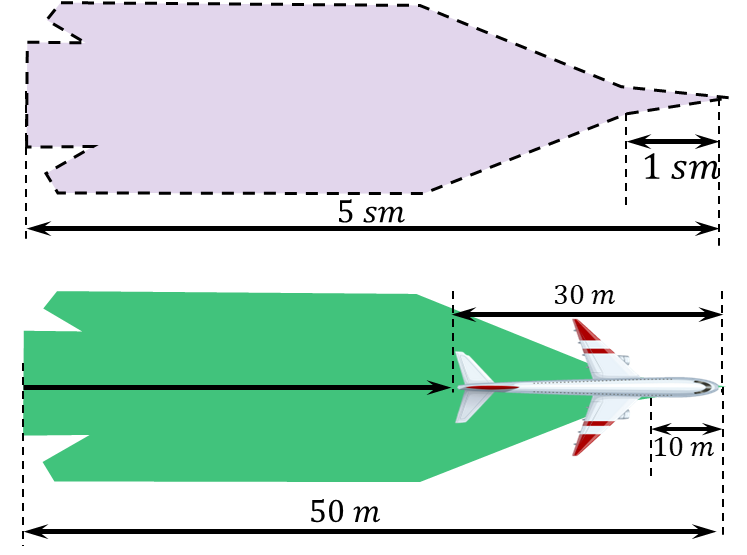
\includegraphics[width=0.3\linewidth]{1.1.1.png}
\end{center}


\item 
The radar measures the angle between the North Pole and the plane's direction and the distance to the aircraft.
At a certain point in time the position of the plane was determined by the following coordinates: angle $\alpha_1 = 44^{\circ}$, distance $R_1 = 100$ km. In a time interval of $5$ seconds after this moment the coordinates of the aircraft were: angle $\alpha_2 = 46^{\circ}$, distance $R_2 = 100$ km. In a Cartesian coordinate system with the y-axis pointing north and the radar at the origin, determine the position of the plane at both points in time and the modulus and direction of the aircraft's velocity. Read the angle in a clockwise direction.

\item A bug flew into the room through an open window. The distance from the bug to the ceiling changed with a speed of $1$ m/s, the distance to the wall opposite to the window changed with a speed of $2$ m/s, to the side wall - with a speed of $2$ m/s. After $1$ s of flight the bug hit the corner between the ceiling and the side wall of the room. Determine the speed of the bug's flight and the position in the window through which it flew into the room. The room is $2.5$ m high, $4$ m wide, and $4$ m long.


\item Counters $A$ and $B$, which register the moment of the arrival of a $\gamma$-quantum, are located at a distance of $2$ m from each other. At a point between them a $\pi_0$ meson decayed into two $\gamma$-quanta. Find the position of this point if counter $A$ detected the $\gamma$-quantum $10^{-9}$ s later than counter $B$. The speed of light is $3 \cdot 10^8$ m/s.

\item Three microphones located on the same straight line at points $A$, $B$, $C$ recorded successively at the moments $t_A > t_B > t_C$ the sound of an explosion that occurred at point $O$, which lies on the segment $AC$. Find the length of the segment $AO$ if $AB = BC = L$. At what point in time did the explosion occur?

\item Athletes run in a column of length $l$ at speed $v$. The coach runs towards them with speed $u < v$. Each athlete, when he reaches the coach, turns around and starts running back with the same speed. What is the length of the column when all the athletes turn around?

\item A submarine diving vertically and uniformly emits sound pulses of duration $\tau_0$. The duration of the pulse reflected from the bottom is $\tau$. The speed of sound in water is $c$. At what speed does the submarine dive?

\item The conveyor belt has speed $w$. Above the belt moves a machine, throwing $\nu$ balls per unit time. The balls stick to the belt. A ball counter with a photocell counts only the balls that have passed directly under it. How many balls will the counter count in a unit of time if the speed of the machine is $v < w$, the speed of the counter is  $u < w$?


\item a. A rod of length $l$ is made of explosive material. The detonation velocity (the rate of involvement in the explosion of new parts of the explosive) is equal to $v$, and the rate of spreading of the products of the explosion is $u < v$. How does the region occupied by the products of the explosion change with time if the rod is detonated at one end? Make a drawing.

b. From the same explosive material it is necessary to make such a thin-walled conical shell so that when detonating it from the top, the products of the explosion simultaneously hit the rod on the axis of the cone. What angle between the axis of the cone and the generatrix should be chosen?

\item A bus is driving along a straight highway at constant speed $v$. You have noticed the bus when it was at some point $A$. From what area near the highway can you catch up with this bus if your running speed is $u < v$? Draw this area for $u = v/2$.

\item A supersonic airplane is flying horizontally. Two microphones on the same vertical at a distance $l$ from each other register the arrival of sound from an airplane flying over the microphones with a time lag $\Delta t$. The speed of sound in air is $c$. What is the speed of the plane?

\item Two rods intersect at an angle $2 \alpha$ and move with equal velocities $v$ perpendicular to themselves. What is the velocity of the intersection point of the rods? Image 1.1.12



\item From the graph of the dependence of the coordinate on time, graph the dependence of the velocity on time. Image 1.1.13
\begin{center}
    \includegraphics[width=\linewidth]{1.1.12-13.png}
\end{center}

\item Using coordinate-time graphs, find the point in time and place of collision of particles moving along one straight line. The speed of the first particle is $v$, the speed of the second particle is $v/2$. The first particle at time $t = 0$ had coordinate $x = 0$, the second particle at time $t_1$ had coordinate $x = a$.

\item Using the velocity-time graphs, plot the coordinate-time graphs. In cases b and c find the average velocity over a large time.
\begin{center}
    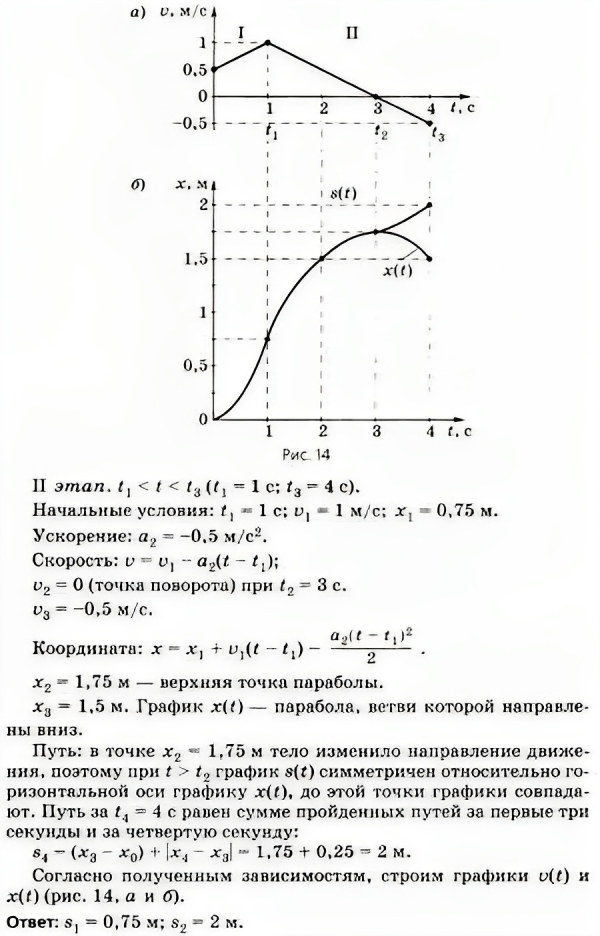
\includegraphics[width=0.5\linewidth]{1.1.15.png}
\end{center}

\item A particle moves in one plane. From the graphs of the time dependence of the velocity projections $v_x$ and $v_y$ plot the trajectory of the particle if $x_{(0)} = 2$ m, $y_{(0)} = 1$ m.
\begin{center}
    \includegraphics[width=0.5\linewidth]{1.1.16.png}
\end{center}

\item The motion of the beam on the oscilloscope screen is described by plots of $x$ and $y$ coordinates versus time. What picture will appear on the screen when $\tau_y = \tau_x$, $\tau_x/3$, $3 \tau_x$? Consider the two cases (see figure 1.1.17). In case a, the horizontal lines are almost invisible on the screen. Why? At what ratio of $\tau_x$ and $\tau_y$ in case b is the trajectory of the beam on the screen closed?

\item The car moves with speed $v$ away from a long wall, moving at an angle $\alpha$ to it. At the moment when the distance to the wall equals $l$, the driver gives a short beep. How far will the car travel before the chauffeur hears the echo? The speed of sound in the air is $c$.

\begin{center}
    \includegraphics[width=0.5\linewidth]{1.1.17-18.png}
\end{center}



\item By what angle will the direction of velocity of the ball change after two elastic impacts on the walls, the angle between which is equal to $\alpha$? How will the ball fly if the angle $\alpha = \pi/2$? The motion occurs in a plane perpendicular to the walls. In an elastic collision with a smooth stationary wall, the angle of incidence of the ball is equal to the angle of reflection.

\item A ball is launched along a pool table with sides $a$ and $b$ from the middle of side $b$. At what angle to the side of the table must the ball begin to move to return to the same point from which it began its movement?

\begin{center}
    \includegraphics[width=0.5\linewidth]{1.1.19-20.png}
\end{center}

\item An angular reflector mounted on the moon rover consists of three mutually perpendicular mirrors. If light, whose velocity $c = (c_x,c_y,c_z)$ falls on the reflector. What components will have the velocity of light after reflection from the mirror located in the $yOz$ plane? After reflection from all three mirrors?
 
\item Inside a fixed smooth-walled cylinder of radius $R$ a small ball is flying, elastically reflecting from the walls so that the minimal distance from it to the cylinder axis is $h$. What fraction of time is the distance from the cylinder axis less than $r$ but greater than $h$?

\begin{center}
    \includegraphics[width=0.5\linewidth]{1.1.21-22.png}
\end{center}
 
\item The shooter tries to hit a disk of radius $R$, which moves from one wall to another at constant modulo velocity so fast that it cannot be tracked. Draw a graph of the probability of hitting the disk as a function of the distance between the aiming point and the left wall.
\begin{center}
    \includegraphics[width=0.5\linewidth]{1.1.23.png}
\end{center}
The shots are fired at height $R$ from the floor perpendicular to the direction of motion of the disc. At what point is the least and most probable shot? What is their value? Consider the cases $L > 4R$, $4R > L > 2R$, where $L$ is the distance between the walls.
\end{enumerate}


\subsection{Variable-speed motion}

\begin{enumerate}[label=1.2.\arabic*]

\item The figure shows the trajectory of an electron that drifts along an interface plane of regions with different magnetic fields. Its trajectory consists of alternating semicircles of radius $R$ and $r$. The velocity of the electron is constant modulo and equals $v$. Find the average velocity of the electron over a long period of time.

\item Two particles at time $t = 0$ have left the same point. Using the velocity-time graphs, determine the coordinates and time of the new meeting of the particles.

\begin{center}
    \includegraphics[width=0.5\linewidth]{1.2.1-2.png}
\end{center}

\item A body for time $t_0$ moves with constant velocity $v_0$. Then its velocity increases linearly with time so that at time $2 t_0$ it is equal to $2 v_0$. Determine the path traveled by the body for time $t > t_0$.

\begin{center}
    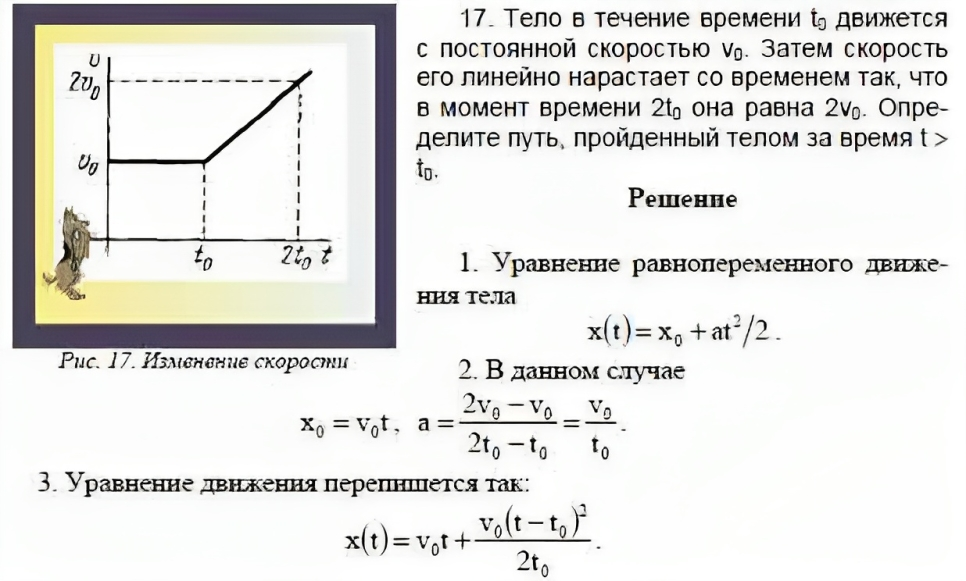
\includegraphics[width=0.3\linewidth]{1.2.3.png}
\end{center}

\item Draw a graph of coordinate versus time for a rectilinear motion that satisfies two conditions simultaneously: 

a. the average speed in the time interval from $2$ to $6$ s is $5$ m/s; 

b. the maximum speed in the same interval is $15$ m/s.

\item When entering a damaged section of the highway, each car in a convoy reduces its speed from $v_1$ to $v_2$. What should be the distance between the cars so that they do not collide? The length of each car is $l$.

\item The graph of the velocity of the body versus time looks like a semicircle. Maximum velocity of the body $v_0$, time of motion $t_0$. Determine the distance traveled by the body.



\begin{center}
    \includegraphics[width=0.3\linewidth]{1.2.6.png}
\end{center}


\item The bus moves for $20$ seconds in a straight line to the stop, passing a distance of $310$ m. Its initial speed is $15$ $\frac{m}{s}$. Prove that the acceleration of the bus changes in direction.

\item . The particle, after leaving the source, flies at a constant speed for a distance $L$, and then decelerates with acceleration $a$. At what speed will the particle have the shortest travel time from its departure to its stop?

\item Migrating fish, having accumulated a reserve of fat in the sea, enter the estuaries of rivers. They do not feed in fresh water, so it is important for them to reach the spawning grounds in the upper reaches of the river with the least weight loss. The consumption of fat for maintaining the basic metabolism in the fish's body per unit of time is $N$, and the additional consumption of $bv^2$ is spent on movement at a speed of $v$. How fast should the fish move so that the fat consumption on the way to the spawning area is minimal? (Pisces can sense this speed perfectly.)

\item From a hemispherical aquarium of radius $R$ filled with water, a volume of liquid $q$ evaporates from a unit of the water surface per unit of time. How long will it take for the water to evaporate?

\item a. In a conical vessel, the water level rises at a constant rate $v_0$. How does the rate of water entering a vessel through a tube of section $s$ depend on time? At time zero, the vessel is empty.

b. A jet of oil hitting the surface of the water spreads over it in a round spot of thickness $h$. How does the speed of movement of the spot boundary depend on time, if the volume of oil $q$ enters per unit of time? At the initial time, the spot radius is zero.

\begin{center}
    \includegraphics[width=0.3\linewidth]{1.2.11.png}
\end{center}

\item A boy inflates a balloon. With a ball radius of $10$ cm, the rate of increase in the radius is $1$ $\frac{mm}{s}$. How much air does the boy exhale every second?

\item " The ship was going at the limit, further acceleration was not provided for by the instructions of the space Fleet. An hour later, the speed increased by a thousand kilometers per second" (Kir Bulychev. Agent KF / / Chemistry and Life. 1984. No. 12, p. 111). Find the acceleration of the ship. How many times does it exceed the acceleration of gravity on Earth?

\item According to the graph of acceleration versus time, set the speed at times $4$ and $15$ s, if at time $1$ s the speed is $3$ $\frac{m}{s}$.

\begin{center}
    \includegraphics[width=0.5\linewidth]{1.2.14.png}
\end{center}

\item The acceleration of the rocket cart from start to stop for the first $6$ seconds is $100$ $\frac{m}{s^2}$, then for $7$ seconds it moves without acceleration, and for the last $3$ seconds the cart has a negative acceleration of $-200$ $\frac{m}{s^2}$ . Plot graphs based on acceleration time, velocity, and coordinates. What is the highest speed of the cart? On what part of the road did the braking occur? What is the total distance traveled by the cart? How can I use the graph of acceleration versus time to check whether the cart has actually stopped?

\item The graphs of the coordinate dependence on time plotted in different time scales for two particles turned out to be the same. One division of the time axis $t$ for the graph of the first particle corresponds to $4$ s, and for the graph of the second — $1$ s. Find the ratio of velocities and the ratio of particle accelerations for point A of the graph.

\item The part of the coordinate-time dependence graph located below the $t$-axis is similar to the part of the graph that is above this axis. Plot graphs based on time, speed, and acceleration. Compare the accelerations for the largest and smallest values of $x$.

\begin{center}
    \includegraphics[width=0.4\linewidth]{1.2.16-17.png}
\end{center}

\item Plot the velocity versus time graph for coordinates and acceleration if $x(0) = 0$.

\item The speedometer scale is $15$ cm long and measures the vehicle speed from zero to $150$ $\frac{km}{h}$. Find the speed of the speedometer indicator if the car is moving at an acceleration of $2$ $\frac{m}{s^2}$.

\begin{center}
    \includegraphics[width=0.5\linewidth]{1.2.18-19.png}
\end{center}

\item The body starts moving from point $A$ and moves first equidistant for time $t_0$, then with the same modulo acceleration — equidistant. After what time from the beginning of the movement, the body will return to point $A$?

\item The scheduled departure time of the train is $12.00$. It's $12.00$ on your watch, but the penultimate car that moves past you during time $t_1$ is already starting to pass by you.
The last car passes you during $t_2$. The train left on time and is moving equidistant. How far behind is your watch?


\end{enumerate}


\subsection{Motion in gravity field. Curvilinear motion}

\begin{enumerate}[label=1.3.\arabic*]

\item Two balls with velocity v are thrown vertically upwards from the same point with time interval $\Delta t$. How long after the second ball leaves, will they collide?

\begin{center}
    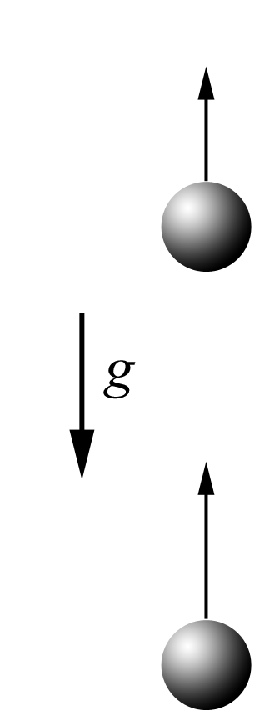
\includegraphics[width=0.2\linewidth]{1.3.1.png}
\end{center}

\item a. From the top point of the circle, a ball begins to slide along a smooth chute at an angle $\varphi$ to the vertical. How long will it take for it to reach the circle, if its diameter is $D$?

b. From point $A$, small beads begin to slide along the spokes with different slopes at the same time without friction. What curve will the beads be on at time $t$?

\begin{center}
    \includegraphics[width=0.5\linewidth]{1.3.2.png}
\end{center}

$\ast$) If the figure for the problem indicates the acceleration of gravity $g$, it is necessary to take into account the gravity field.

\item At what angle to the vertical should a smooth chute be directed from point $A$ so that the ball slides down it to the inclined plane in the shortest time?

\begin{center}
    \includegraphics[width=0.5\linewidth]{1.3.3.png}
\end{center}

\item A free-falling body flew past point $A$ with velocity $v_A$. How fast will it fly past point $B$, which is $h$ below $A$?

\item A stone is thrown at a velocity $v$ at an angle $\varphi$ to the horizon. After what time will the velocity be at the angle $\alpha$ with the horizon?

\item The gun is fired at an angle $\varphi$ to the horizon. Initial velocity of the projectile $v$. The ground surface is horizontal. Find: a) the horizontal and vertical projections of velocity as a function of time; b) the dependence of the $x$ and $y$ coordinates on time; c) the trajectory equation, i.e. the dependence of $y$ on $x$; d) the flight time, the highest altitude and range of the projectile.

\item A ball is launched along a smooth inclined plane at a speed of $v$. How much horizontal distance will it travel before it rolls off the plane? The plane is inclined to the horizon at an angle of $45^\circ$ . The initial velocity of the ball forms an angle of $45^\circ$ with the horizontal edge of the plane.

\item A mortar is fired at objects located on the mountainside. At what distance from the mortar will the mines fall if their initial velocity is $v$, the angle of inclination of the mountain is $\alpha$, and the angle of fire relative to the horizon is $\beta$?

\begin{center}
    \includegraphics[width=0.5\linewidth]{1.3.7-8.png}
\end{center}

\item At what speed should a projectile fly out of a cannon at the moment of rocket launch in order to hit a rocket starting vertically with acceleration $a$? The distance from the gun to the rocket launch site is $L$, the gun fires at an angle of $45^\circ$ to the horizon.

\item The duck was flying in a horizontal straight line with a constant speed $u$. An inexperienced "hunter" threw a stone at it, and the throw was made without pre-emption, i.e. at the time of the throw, the speed of the stone $v$ was directed just at the duck at an angle $\alpha$ to the horizon. At what height did the duck fly, if the rock still hit it? 

\item From the opening of the hose covered with a finger, two jets are shot at an angle $\alpha$ and $\beta$ to the horizon with the same initial velocity $v$. At what horizontal distance from the hole will the jets intersect?

\begin{center}
    \includegraphics[width=0.5\linewidth]{1.3.10-11.png}
\end{center}

\item From a hose lying on the ground, water shoots at an angle of $45^\circ$ to the horizon with an initial velocity of $10$ $\frac{m}{s}$. The cross-sectional area of the hose opening is $5$ $cm^2$ . Determine the mass of the jet in the air.

\item The projectile flew out of the gun and hit a point with $x$ coordinates horizontally and $y$ coordinates vertically. Initial velocity of the projectile $v$. Find: a) the tangent of the angle formed by the gun barrel with the horizon; b) the boundary of the area of possible hit of the projectile; c) the lowest initial velocity of the projectile at which it can hit the point with coordinates $x$, $y$. Note. For the solution, use the trigonometric identity $\frac{1}{cos^2 \varphi} = tg^2 \varphi + 1$.

\item Two bodies with the same initial velocity $v$ are thrown from the same place with a time interval $\Delta t$ at an angle $\varphi$ to the horizon. How does the first body move relative to the second? Why does the relative velocity depend only on $\Delta t$?

\item A ball is launched along the inner surface of a smooth vertical cylinder of radius $R$ at an angle $\alpha$ to the vertical. What initial speed does it need to be told to return to its starting point?

\item A ball flies into a tube of length $l$, inclined at an angle $\alpha$ to the horizon, with a horizontal velocity $v$. Determine the time of the ball's stay in the pipe, if the ball hits its walls elastic.

\item In a rectangular box, elastically hitting the bottom and the right wall, a ball jumps back and forth along one trajectory. The time interval between hitting the bottom and the wall is $\Delta t$. The bottom of the box forms an angle $\alpha$ with the horizon. Find the speed of the ball immediately after hitting.

\begin{center}
    \includegraphics[width=0.5\linewidth]{1.3.16-17.png}
\end{center}

\item In a spherical hole, a ball jumps, elastically hitting its walls at two points located on the same horizontal line. The time interval between strokes when moving the ball from left to right is always equal to $T_1$, and when moving from right to left-$T_2 \ne T_1$. Determine the radius of the hole.

\begin{center}
    \includegraphics[width=0.3\linewidth]{1.3.18.png}
\end{center}

\item What is the minimum speed required for a stone thrown by a boy to fly between height $H$ and length $L$, if the throw is made from height $h$ and the boy can choose any place to throw?

\item Determine the speed and acceleration that points on the Earth's surface at the equator and in St. Petersburg have due to the Earth's participation in the diurnal rotation. Take the Earth's radius as $6400$ km. The latitude of St. Petersburg is $60^\circ$ .

\item At what speed should a satellite fly in order to move in a circle while "falling" to the Earth with acceleration $g$? Assume the orbit radius $R = 6400$ km and $g = 10$ $\frac{m}{s^2}$ .

\item Planes fly in a straight line towards each other at the same speed $v$. The maximum range of detection of each other by them $l$. One plane, after detecting the other, makes a $U$-turn without changing the speed module, and flies parallel to the second plane. At what constant acceleration will the planes lose sight of each other at the end of the turn?

\item A small body moves at a constant velocity $v$ along a trajectory consisting of two smoothly connected arcs of circles of radius $R$ and $\frac{R}{3}$. Plot the acceleration vectors at the marked points of the trajectory.

\begin{center}
    \includegraphics[width=0.5\linewidth]{1.3.22-23.png}
\end{center}

\item At a time when the particle velocity is $10^6$ $\frac{m}{s}$, its acceleration is $10^4$ $\frac{m}{s^2}$ and is directed at an angle of $30^\circ$ to the velocity. How much will the speed increase in $10^{-2}$ seconds? At what angle will the speed direction change? What is the angular velocity of rotation of the velocity vector at this moment?

\item A small body moves along a circle of radius $r$ at a speed that increases linearly in time according to the law $v = kt$. Find the dependence of the total acceleration of the body on time.

\item The edge of a smooth horizontal table is rounded along a circle of radius $r$. What is the lowest speed you need to put a small body on the table, so that it reaches the rounding, immediately flew along the parabola?

\begin{center}
    \includegraphics[width=0.5\linewidth]{1.3.26.png}
\end{center}

\item A spherical tank standing on the ground has a radius of $R$. What is the lowest speed at which a rock thrown from the ground can fly over the reservoir just by touching its top?

\item Projectiles fly out at an initial velocity of $600$ $\frac{m}{s}$ at an angle of $30^\circ$, $45^\circ$, $60^\circ$ to the horizon. Determine the radius of curvature of the projectile trajectory at their highest and starting points.

\item To save space, the entrance to one of the highest bridges in Japan is arranged in the form of a spiral line that wraps around a cylinder of radius $R$. The roadbed forms an angle $\alpha$ with the horizontal plane. What is the acceleration of a car moving along it at a constant modulo velocity $v$?

\item The projectile leaves the cannon at a velocity $V$ at an angle $\alpha$ to the horizon. What time does the projectile approach the cannon?



\end{enumerate}


\subsection{Galileo's transformations}

\begin{enumerate}[label=1.4.\arabic*]

\item The initial positions and velocities of the two ships are shown in the figure. Ships move without acceleration. How do I find the smallest distance between them?

\item In the figure, the velocities of six hares released by the old Mazai are shown in a coordinate system that is stationary relative to the Mazai. Try drawing the velocities of Mazai and the other hares in a coordinate system that is stationary relative to hare $1$.

\begin{center}
    \includegraphics[width=0.5\linewidth]{1.4.1-2.png}
\end{center}

\item One of the dust cloud particles (particle $A$) is at rest, and all the others are flying away from it in different directions with velocities proportional to the distances from them to particle $A$. What motion pattern will an observer detect when moving with particle $B$?

\item From corner $A$ of a square raft, a dog jumped into the water and swam around the raft. Draw the dog's trajectory relative to the shore if it is swimming along the sides of the raft, and its speed relative to the water is $\frac{4}{3}$ of the speed of the river current.

\begin{center}
    \includegraphics[width=0.3\linewidth]{1.4.4.png}
\end{center}

\item a. Due to air resistance, raindrops fall at a constant velocity $v$ perpendicular to the ground surface. How is it necessary to position a cylindrical bucket on a platform moving at a speed of $u$ so that drops do not fall on its walls? 

b. At a wind speed of $10$ $\frac{m}{s}$, raindrops fall at an angle of $30^\circ$ to the vertical. At what wind speed will the drops fall at an angle of $45^\circ$ ?

\item The buoy is a sailing sled. He can only move along the line along which his skates are directed. The wind blows at a speed $v$ perpendicular to the direction of movement of the buoy. The sail is $30^\circ$ with the direction of travel. What speed can not exceed the buoy in this wind?

\begin{center}
    \includegraphics[width=0.3\linewidth]{1.4.6.png}
\end{center}

\item What is the duration of a plane's flight from Novosibirsk to Moscow and back in a straight line, if the wind blows at an angle $\alpha$ to the track at a speed $u$ during the entire flight? The speed of the aircraft relative to the air $v$, the length of the route $L$. In which wind direction is the maximum flight duration?

\item In case of an elastic impact of a body against a fixed wall, its velocity $v$ changes only in the direction. Determine the change after the impact of the velocity of this body, if the wall is moving: a) at a speed $u$ towards the body; b) at a speed $w < v$ in the direction of movement of the body.

\item The body hits the wall with velocity $v$ and angle $\alpha$ to the line perpendicular to the wall. Determine the velocity of the body after an elastic impact if the wall is: a) stationary; b) moving perpendicular to itself at a speed $w$ towards the body; c) moving at an angle $\beta$ to the line perpendicular to it at a speed $w$ towards the body.

\begin{center}
    \includegraphics[width=0.5\linewidth]{1.4.8-9.png}
\end{center}

\item Inside a sphere of radius $R$ moving at speed $u$, there is a ball of radius $r$, which at the moment when it passes through the center of the sphere, has a velocity $v$ perpendicular to the velocity $u$. The mass of the sphere is much greater than the mass of the ball. Determine the frequency with which the ball hits the wall of the sphere. The blows are absolutely elastic.

\item The body is dropped over the slab at a height $h$ from it. The slab moves vertically upwards at a speed of $u$. Determine the time between two consecutive impacts of the body on the slab. The blows are absolutely elastic.

\item A body flies horizontally at speed $v$ into the space between two vertical walls that move at speed $u$. Determine the speed of the body after the $n$-th impact on the front wall. Distance between walls $L$. The blows are absolutely elastic.

\begin{center}
    \includegraphics[width=0.3\linewidth]{1.4.12.png}
\end{center}

\item A gear of radius $R$ is placed between two parallel gear racks. The slats move at a speed of $v_1$ and $v_2$ towards each other. What is the gear speed?

\item A nucleus traveling at speed $v$ splits into two identical fragments. Determine the maximum possible angle $\alpha$ between the velocities of one of the fragments and the vector $v$, if the fragments have a velocity $u < v$ during the decay of a resting nucleus.

\item There is a bundle of identical nuclei moving with velocity $v$. The nuclei in the beam spontaneously divide into pairs of identical fragments. The velocity of the fragments moving in the direction of the beam is $3v$. Find the velocity of the fragments moving in the direction perpendicular to the beam.

\item Two beams of particles moving with the same modulo velocity $v$ intersect at an angle $\alpha$. Particle collisions occur in a limited area. Let's move on to the reference frame, where the particle velocities are equal in modulus and opposite in direction. It would seem that now the intersection area is the entire volume of beams, and therefore the number of collisions per unit time should be greater. Explain the resulting contradiction.

\begin{center}
    \includegraphics[width=0.3\linewidth]{1.4.16.png}
\end{center}

\item It is raining heavily. Drop rate $u$. The ball slides on the asphalt at a speed of $v$. How many times in the same period of time does it get more drops than the same, but stationary ball? Does the answer change if the ball is not round?

\item A boy who can swim at half the speed of a river wants to swim across the river so that he is not carried downstream as much as possible. At what angle to the shore should he swim? How far will it go if the river is $200$ m wide?




\end{enumerate}


\subsection{Motion with constraints}

\begin{enumerate}[label=1.5.\arabic*]
 
 
\item The speed of the load $A$ is equal to $v_A$. What is the speed of load $B$?

\item The angular velocity of the coil is $\omega$, the radius of the inner cylinder is $r$, and the radius of the outer cylinders is $R$. What are the velocities of the coil and load axis relative to the ground?

\item A wedge with an angle of $30^\circ$ lies on a horizontal plane. A vertical rod descending at a speed of $v$ causes the wedge to slide along this plane. What is the speed of the wedge?

\begin{center}
    \includegraphics[width=0.6\linewidth]{1.5.1-2-3.png}
\end{center}

\item A coin is placed on a wedge with an angle $\alpha$. With what minimum acceleration should the wedge move along the horizontal plane so that the coin falls freely down?

\item The speed of a coin sliding off a wedge is shown in the figure. Use a graphical plot to find the speed of the wedge.

\item A flat solid body rotates around an axis perpendicular to its plane. The coordinates of the initial position of points $A$ and $B$ of this body are ($-1$, $2$) and ($3$, $1$), and the final position is ($-3$, $1$) and ($-2$, $-3$). Use a graphical plot to find the coordinates of the rotation axis.

\item a. The velocity of a point $A$ of a solid body is equal to $v$ and forms an angle of $45^\circ$ with the direction of the straight line $AB$. The velocity of point $B$ of this body is $u$. Determine the projection of the velocity of point $B$ on the direction $AB$.

b. The velocities of points $A$ and $B$ of a solid body are equal to $v$. The velocity of a point $C$ in the plane of a straight line $AB$ and a vector $V$ is $u > v$. Find the velocity projection of point $C$ on the axis perpendicular to the specified plane.

\begin{center}
    \includegraphics[width=0.6\linewidth]{1.5.5.7.png}
\end{center}

\item Plot the trajectories of the points of the wheel rolling without slipping on the rail. Consider cases where the points are at a distance from the wheel axis: $r > R$, $r = R$, $r < R$. Find the acceleration of these points if the wheel axis is moving at a constant speed $v$. Find the radius of curvature of the trajectory of a point located in the highest and lowest positions at a distance $r \ne R$ from the wheel axis.

\item The thread wound on the axis of the coil is pulled at a speed $v$ at an angle $\alpha$ to the horizon. The reel rolls along a horizontal plane without slipping. Find the speed of the axis and the angular velocity of rotation of the coil. At what angles does the $\alpha$ axis move to the right? to the left? The thread is so long that the angle $\alpha$ does not change when moving.

\begin{center}
    \includegraphics[width=0.5\linewidth]{1.5.8-9.png}
\end{center}

\item On the inner surface of a fixed cylinder of radius $2r$, a wheel of radius $r$ rolls without slipping. Find the path of the wheel rim point.

\item a. The moon is always facing the Earth on one side. How many revolutions will it make around its axis during a complete revolution around the Earth? 

b. How much shorter are sidereal days than solar days on average? The Earth goes around the Sun in $365$, $25$ sunny days.

\item A bead can move along a ring of radius $R$, pushed by a spoke that rotates uniformly with angular velocity $\omega$ in the plane of the ring. The axis of rotation of the spoke is located on the ring. Determine the acceleration of the bead.

\item The rope tied to the boat is pulled by the free end so that it does not sag. The boat moves at a constant speed $v$, forming at some point in time an angle $\alpha$ with the length of rope located between the pole and the boat. How fast should the free end of the rope be pulled at this point in time?

\begin{center}
    \includegraphics[width=0.5\linewidth]{1.5.10-12-13.png}
\end{center}

\item Four turtles are located at the vertices of a square with side $a$. They start moving simultaneously at a constant modulo velocity $v$. Each turtle moves clockwise in the direction of its neighbor. Where will the turtles meet and after what time?

\item Plot an approximate graph of the speed of point $B$ as a function of time, if the speed $v_A$ of point $A$ is constant. Find the formula for this relationship if $x(0) = 0$.

\item The rod rests its ends on the sides of a right angle. The upper end of the rod is lifted at a speed of $v$. Find how the speed of its lower end depends on time. Take the moment when the upper end is at the top of the corner as the beginning of the time reference. Rod length $L$.

\begin{center}
    \includegraphics[width=0.5\linewidth]{1.5.15-16.png}
\end{center}

\item The log, resting its lower end in the corner between the wall and the ground, touches the bottom of the truck at a height $H$ from the ground. Find the angular velocity of the log as a function of the angle $\alpha$ between it and the horizontal if the truck is moving away from the wall at speed $v$.

\item The rod, with one end pivotally fixed on a horizontal plane, lies on the cylinder. Angular velocity of the rod $\omega$. There is no slippage between the cylinder and the plane. Find the dependence of the angular velocity of the cylinder on the angle $\alpha$ between the rod and the plane.

\begin{center}
    \includegraphics[width=0.5\linewidth]{1.5.17-18.png}
\end{center}

\item A spherical buoy of radius $R$ is attached to the bottom of the reservoir. The water level in the reservoir rises at a speed $u$. What is the speed of movement of the boundary of the flooded part of the buoy on its surface at the moment when the water level is $h$ above the center of the buoy?

\begin{center}
    \includegraphics[width=0.3\linewidth]{1.5.19.png}
\end{center}

\item The reel of tape is played back during time $t$ at the film drawing speed $v$. The initial radius of the reel (with film) is $R$, and the final radius (without film) is $r$. What is the thickness of the film?

 
 
 
\end{enumerate}



\section{Dynamics}

\subsection{Newton's Laws}

\begin{enumerate}[label=2.1.\arabic*]


\item According to reliable information, Baron Munchausen once got bogged down in a swamp and pulled himself out by the hair. What laws of physics did the baron break?

\item The puck, which was sliding on the ice, stopped after a time $t = 5$ s after hitting the stick at a distance $l = 20$ m from the place of impact. The mass of the washer is $m = 100$ g. Determine the friction force acting on the washer.

\item In a cathode-ray tube, electrons with an initial horizontal velocity $v$ fly into the region of an electric field of length $l$, where they are affected by a vertical force from charged deflecting plates. What is this force equal to if the electrons hitting the screen are displaced by a distance $y$ compared to the case of uncharged plates? The screen is located at a distance $L$ from the center of the area of action of the electric force. The mass of the electron is $m_e$.

\item The load is secured to the cart by four strung threads. The tension force of horizontal threads is $T_1$ and $T_2$, respectively, and that of vertical threads is $T_3$ and $T_4$. How fast does the cart move along the horizontal plane?

\begin{center}
    \includegraphics[width=0.5\linewidth]{2.1.3-4.png}
\end{center}

\item What force acts in the cross-section of a homogeneous rod of length $l$ at a distance $x$ from the end to which the force $F$ is applied along the rod?

\item Two bodies of mass $m_1$ and $m_2$ are connected by a thread that can withstand the tension force $T$. Forces $F_1 = \alpha t$ and $F_2 = 2 \alpha t$ are applied to the bodies, where $\alpha$ is a constant coefficient, and $t$ is the time of action of the force. Determine at what point in time the thread will break.

\begin{center}
    \includegraphics[width=0.5\linewidth]{2.1.5-6.png}
\end{center}

\item To measure the mass of an astronaut on an orbital station, a movable seat of known mass $m_0$ attached to a spring is used. With the same initial spring deformation (compression), the empty seat returns to its original position after a time $t_0$, but if the astronaut is on the seat, it returns after a time $t > t_0$. What is the mass of an astronaut?

\item The dynamometer consists of two cylinders connected by a light spring. Find the mass ratio of these cylinders if the dynamometer shows the force $F$ when the forces $F_1$ and $F_2$ are applied to them.

\begin{center}
    \includegraphics[width=0.5\linewidth]{2.1.8.png}
\end{center}

\item To test the equipment in zero-gravity conditions, the container is thrown up by a pneumatic piston device located at the bottom of the evacuated shaft. The piston acts on the container for a time $\Delta t$ with a force $F = nmg$, where $m$ is the mass of the container with the equipment. How long will it take for the container to fall to the bottom of the mine? How long does the zero-gravity state last for the equipment, if $\Delta t = 0.04$ s, and $n = 125$?

\item Astronauts wearing spacesuits train in water to prepare for work in zero gravity. In this case, the force of gravity acting on them is balanced by the buoyant force. What is the difference between such" weightlessness " and the real one?

\item Find the acceleration of loads and tension forces of threads in the system shown in the figure. The block and threads are weightless, there is no friction.

\item The painter works in a suspended cradle. He needed to get up quickly. He begins to pull the rope with such force that the force of his pressure on the floor of the cradle is reduced to $400$ H. Cradle weight $12$ kg, painter weight $72$ kg. What is the acceleration of the cradle?

\item A system of three identical balls connected by identical springs is suspended on a thread. The thread is burned out. Find the acceleration of the balls immediately after burning the thread.

\begin{center}
    \includegraphics[width=0.5\linewidth]{2.1.11-12-13.png}
\end{center}

\item Bodies of mass $m_1$ and $m_2$ are connected by a spring of stiffness $k$. A constant force $F$ acts on the body of mass $m_2$, directed along the spring to the body of mass $m_1$. Find out how much the spring is compressed, if there are no other external forces, and the vibrations have already stopped. What will be the acceleration of bodies immediately after the termination of the force $F$?

\item The body of mass m is connected by two springs of stiffness $k_1$ and $k_2$ with fixed walls, the springs are not initially deformed. When vibrations occur, the greatest acceleration of the body is $a$. Find the maximum deviation of the body from the equilibrium position and the maximum forces with which the springs act on the walls.

\begin{center}
    \includegraphics[width=0.5\linewidth]{2.1.14-15.png}
\end{center}

\item The body of mass $m$ is attached to two consecutive springs of stiffness $k_1$ and $k_2$. A constant force $F$ is applied to the free end of the spring chain. What is the total elongation of the springs, if the vibrations have already stopped?

\begin{center}
    \includegraphics[width=0.5\linewidth]{2.1.16.png}
\end{center}

\item A light magnet with a hook on a vertical steel plate remains stationary as long as the weight suspended from it does not exceed $m_0$ in mass. What is the magnetic force if the coefficient of friction of the magnet on steel is equal to $\mu$? With what acceleration does the magnetic suspension slide, if the mass of the load is $m > m_0$?

\begin{center}
    \includegraphics[width=0.3\linewidth]{2.1.17.png}
\end{center}

\item A body located on a horizontal plane is pulled by the thread in the horizontal direction. Draw a graph of the dependence of the friction force acting on the body from the plane on the tension force of the thread. Initially, the body is motionless. Body weight $10$ kg, coefficient of friction $0.51$.

\item If you press your finger on a ballpoint pen resting on a hard surface, while simultaneously tilting it, then as long as the pen forms a small angle with a perpendicular to the surface, it will obediently follow the finger of the hand. As soon as the handle tilt angle exceeds a certain maximum value of $\alpha_{max}$, it will slip out from under your finger, no matter how hard or weak you press it. Experiment for yourself and estimate the coefficient of friction between the ball of the pen and the surface on which it rests.

\item A bar of mass $m$ is placed on the horizontal board. The board is slowly tilted. Determine the dependence of the friction force acting on the bar on the angle of inclination of the board $\alpha$. Coefficient of friction $\mu$.

\item The belt lift forms an angle $\alpha$ with the horizon. With what maximum acceleration can a box be lifted on such a lift, if the coefficient of friction is equal to $\mu$? The tape doesn't bend.

\item After what time will the velocity of a body that has been sent up an inclined plane with velocity $v$ be equal to $v$ again? Coefficient of friction $\mu$, the angle between the plane and the horizon $\alpha$, $tg \alpha > \mu$.

\item A body of mass $m$ lying on a horizontal plane is affected by a force $F$ at an angle $\alpha$ to the horizon. Coefficient of friction $\mu$. Find the acceleration of the body if it does not detach from the plane.

\item The cylinder slides along the chute, which has the form of a dihedral angle with the solution $\alpha$. The edge of a dihedral angle is inclined at an angle $\beta$ to the horizon. The planes of a dihedral angle form identical angles with the horizon. Determine the acceleration of the cylinder. Coefficient of friction between the cylinder and the chute surface $\mu$.

\item A thread spanned over a block with a fixed axis is passed through a slot. At the ends of the thread are suspended loads, the mass of which is $m_1$ and $m_2$. Determine the acceleration of loads if a constant frictional force $F_{tr}$ acts on the thread from the side of the slot when it moves.

\item On the wooden gangplank forming an angle $\alpha$ with the horizon, a box is dragged by a rope tied to it. Coefficient of friction of the box on the gangway $\mu$. At what angle to the horizon should the rope be pulled in order to pull the box with the least effort?

\item A person of mass $m_1$, remaining in place, pulls a weight of mass $m_2$ by the rope. The coefficient of friction on the horizontal plane is equal to $\mu$. At what is the lowest tension force of the rope, the load will start from its place? At what angle to the horizontal plane should the rope be directed?

\begin{center}
    \includegraphics[width=0.5\linewidth]{2.1.25-27.png}
\end{center}

\item On an icy section of the highway, the coefficient of friction between the wheels and the road is ten times less than on an un-icy one. How many times do you need to reduce the speed of the car so that the braking distance on an icy section of the highway remains the same?

\item A car with a powerful engine, starting from a place, gains a speed of $72$ $\frac{km}{h}$ in $5$ seconds. Find the coefficient of friction between the wheels and the road. What is the shortest braking distance of a car that has reached this speed?

\item A body of mass $m_1$ lies on a board of mass $m_2$ located on a smooth horizontal plane. Coefficient of friction between the body and the board $\mu$.

a. What force should be applied to the board so that the body slides off it? How long will it take for a body to slide if a force $F_0$ is applied to the board and the length of the board is $l$?

b. With what acceleration do the body and board move if the force $F_0$ acts on the body of mass $m_1$?

\begin{center}
    \includegraphics[width=0.5\linewidth]{2.1.30.png}
\end{center}

\item The cargo system shown in the figure is located on a smooth horizontal table. The lower right weight is pulled along the table with a force of $F$, as indicated in the figure. The coefficient of friction between loads of mass $m_1$ and $m_2$ is equal to $\mu$. Find the acceleration of all loads in the system.

\item Determine the force acting on the vertical wall from the side of the wedge, if a weight of mass $m$ is placed on it. Angle at the base of the wedge $\alpha$. Coefficient of friction between the load and the wedge surface $\mu$. There is no friction between the floor and the wedge.

\begin{center}
    \includegraphics[width=0.5\linewidth]{2.1.31-32.png}
\end{center}

\item Why does the speed of raindrops not depend on the height of clouds and strongly depends on the size of drops?

\item The air resistance force acting on the cyclist is proportional to the square of the cyclist's speed: $f = \alpha v^2$ . On a horizontal road, the maximum speed of a cyclist is approximately $20$ $\frac{m}{s}$. Estimate the proportionality coefficient $\alpha$ if the mass of the cyclist together with the bike is $70$ kg, and the coefficient of friction between the wheels and the road is $0.4$.

\item The mass of the balloon together with the rope dragging on the ground is $m$; the buoyant force acting on the balloon is $F$; the coefficient of friction of the rope on the ground is $\mu$. The air resistance force acting on the balloon is proportional to the square of the balloon's velocity relative to the air: $f = \alpha v^2$ . Find the speed of the ball relative to the ground if there is a horizontal wind blowing at speed $u$.

\begin{center}
    \includegraphics[width=0.5\linewidth]{2.1.35.png}
\end{center}

\item The velocity of a body of mass $m$ in a viscous liquid decreases with the distance $l$ traveled according to the law $v = v_0 - \beta l$, where $v_0$ is the initial velocity, and $\beta$ is a constant coefficient. How does the viscous friction force acting on a body from the fluid side depend on the velocity of the body?

\item The force of air resistance acting on raindrops is proportional to the product of the square of the droplet velocity and the square of their radius: $f = A \rho_0 r^2 v^2$, where $\rho_0 \approx 1.3$ $\frac{kg}{m^3}$ is the air density, and the dimensionless coefficient A for round drops is of the order of $1$. Which drops, large or small, fall to the ground with faster speed? Estimate the velocity of a drop of radius $r = 1$ mm when it falls from a great height.

\item The air resistance force acting on fog drops is proportional to the product of the radius and velocity: $f = \gamma rv$. Drops of radius $r = 0.1$ mm, falling from a great height, have a speed of about $1$ $\frac{m}{s}$ near the ground. What speed will drops have if their radius is half as large? ten times less?

\item The drag force of a liquid or gas, proportional to the square of the velocity of a moving body, is associated with the formation of vortices in the medium near the surface of this body. The drag force, which is proportional to the speed of a moving body, is associated with the slippage of the layers of the medium when it flows around this body. Both phenomena occur simultaneously. Why, however, can only one type of resistance be taken into account under certain conditions? Based on the data of the previous two problems, estimate at what value the product of the radius of a round drop and its velocity is, both types of air resistance are comparable in their effect on the movement of the drop.

\item The horizontal conveyor belt moves at a speed of $u$. A washer flies into the tape at a tangent to it, the initial velocity $v$ of which is perpendicular to the edge of the tape. Find the maximum width of the tape at which the washer will reach its other edge if the coefficient of friction between the washer and the tape is $\mu$.

\item Which washer, rotating around its axis or not rotating, will go the longest way to stop on a rough horizontal surface? The initial velocity of the puck centers is the same.

\begin{center}
    \includegraphics[width=0.5\linewidth]{2.1.40-41.png}
\end{center}

\item Why is it easier to pull out a nail that is firmly embedded in a log if you simultaneously rotate it around its own axis when pulling it out?

\item The horizontal axis of radius $R$, which rotates at an angular velocity $\omega$, is compressed by a sleeve equipped with a counterweight so that it does not rotate when moving along the axis. Determine the steady-state velocity of the bushing under the action of a force $F$ applied to it along the axis. Maximum friction force of the axle against the bushing $F_{tr} > F$.

\item Determine the steady-state velocity of a body on an inclined plane that changes one direction of its velocity $u$ to the opposite direction with high frequency. The direction of movement of the plane is shown in the figure. Coefficient of friction $\mu$, angle of inclination of the plane $\alpha$, $tg \alpha < \mu$.

\begin{center}
    \includegraphics[width=0.5\linewidth]{2.1.43-44.png}
\end{center}

\item A coin is placed on a plane whose slope tangent is equal to the coefficient of friction. In the horizontal direction along the plane, the coin was given a velocity $v$. Find the steady speed of the coin.

\item Two bodies of the same mass connected by a thread slide along an inclined plane. Thread tension force $T$. There is no friction between one body and the board. Determine the friction force between the board and another body.

\item Find the acceleration of the bodies of the system shown in the figure. The force $F$ is applied in the direction of the thread to one of the bodies of mass $m$. The thread sections on both sides of the light block attached to the body of mass $M$ are parallel.

\item A wedge of mass $m_2$ with an angle $\alpha$ is inserted between two identical smooth bars of mass $m_1$. Determine the acceleration of bodies.

\item A load is suspended from the free end of the thread attached to the wall and thrown over the roller. The roller is fixed on a bar of mass $m_0$, which can slide along a horizontal plane without friction. At the initial moment, the thread with the load is deflected from the vertical by an angle $\alpha$ and then released. Determine the acceleration of the bar if the angle formed by the thread with the vertical does not change during the movement of the system. What is the weight of the cargo?

\item On a smooth horizontal plane there is a wedge with an angle $\alpha$ at the base. A body of mass $m$ placed on a wedge descends with acceleration directed at an angle $\beta > \alpha$ to the horizontal. Determine the mass of the wedge.

\begin{center}
    \includegraphics[width=0.5\linewidth]{2.1.49-50.png}
\end{center}

\item A heavy slab was placed on two skating rinks of different radii. It forms an angle $\alpha$ with the horizon. Find the acceleration of this slab. There is no slippage. Ignore the mass of ice rinks.

\item Acceleration of stars that are part of a binary star, $a_1$ and $a_2$. What is the mass of the second star, if the mass of the first is $m_1$?

\item A dumbbell (two balls of mass m each connected by a weightless rod) was placed in a spherical cavity as shown in the figure. Determine the pressure force of the balls on the walls immediately after the dumbbell is released. The radius of the dumbbell balls is much smaller than the radius of the sphere.

\begin{center}
    \includegraphics[width=0.5\linewidth]{2.1.51-53.png}
\end{center}

\item Electrons moving in a circle of any radius around a charged filament have the same velocity $v$. The mass of the electron is $m_e$. How does the force exerted by the filament on the electron depend on the distance between the electron and the filament? Describe qualitatively the initial segment of the trajectory along which the electron will move, if its speed when moving around a circle suddenly becomes slightly less than $v$? a little more than $v$?

\item Two balls of mass $m$ each, connected by a thread of length $l$, move at a speed $v$ along a horizontal table in the direction perpendicular to the thread connecting them (the thread does not sag). The middle of the thread hits the nail. What is the tension force of the thread immediately after this?

\item A body of mass $M$ is connected by a thread of length $l$ to the axis around which it orbits with angular velocity $\omega$. Find the tension force of the thread. The size of the body is small, and gravity is negligible. Replace the thread with a uniform rope of mass $m$ and find its tension force at a distance $x$ from the axis of rotation.

\item A small bead is placed on a smooth wire ring of radius $R$, located vertically. The ring rotates with an angular velocity $\omega$ around a vertical axis passing through the ring diameter. Where is the bead located?

\item To a heavy ball suspended on a thread of length $l$, a second heavy ball is suspended on a thread of the same length. When the balls rotate around a vertical axis passing through the upper point of the suspension, both threads lie in the same plane and form constant angles $\alpha$ and $\beta$ with the vertical. Find the angular velocity of rotation of the balls.

\begin{center}
    \includegraphics[width=0.5\linewidth]{2.1.57-58.png}
\end{center}

\item A load of mass $m$, attached by a spring of stiffness $k$ to an axis, moves around this axis along a circle of radius $R$ with an angular velocity $\omega$. What is the length of an undeformed spring?

\item From a thin rubber harness of mass $m$ and stiffness $k$, a ring of radius $R_0$ was made. This ring was spun around its axis. Find the new radius of the ring if the angular velocity of its rotation is $\omega$.

\item An annular chain of mass $m$ is placed on a horizontal disk of radius $R$. The tension force of the put-on chain is $T$. Find the coefficient of friction between the disk and the chain if the chain falls off when the disk rotates with an angular velocity equal to or greater than $\omega$.

\item The aircraft makes a turn, moving along a horizontal circle of radius $R$ at a constant speed $V$. What is the angle of the plane of the plane's wings with the horizon?

\begin{center}
    \includegraphics[width=0.5\linewidth]{2.1.61-62.png}
\end{center}

\item A horizontal disk begins to spin around its axis with a linearly increasing angular velocity $\omega = \varepsilon t$ in time. At what angular velocity will a body located at a distance $r$ from the disk axis begin to slide off it, if the coefficient of friction between them is equal to $\mu$?

\item At what maximum speed can a motorcyclist ride on a horizontal plane, describing a circle of radius $R$, if the coefficient of friction is equal to $\mu$? What angle should it deviate from the vertical? How many times will the maximum permissible speed of a motorcyclist increase when driving on an inclined track with an angle of inclination $\alpha$ to the horizon compared to the maximum permissible speed when driving on a horizontal track with the same turning radius and the same coefficient of friction?

\item A skater on an ice track tries to turn as close to the inside edge as possible. A cyclist on a bike track, on the contrary, passes the bend as far as possible from the inner edge. How can we explain this difference in turn passing tactics? The bike track profile gets steeper and steeper as you move away from the inner edge of the track.

\item In a circus ride, a motorcyclist moves along the inner surface of a sphere of radius $R$. As it accelerates, it begins to describe a horizontal circle in the upper hemisphere. After that, for greater effect, the lower hemisphere is removed. Determine the minimum speed of the rider if the coefficient of tire friction on the surface of the sphere is $\mu$, and the angle between the vertical and the direction to the rider from the center of the sphere is $\alpha$.

\item At what angular velocity should a horizontally positioned cylinder rotate around its axis so that small particles inside the cylinder do not slide off its surface? The coefficient of friction between the cylinder surface and the particles is $1$, the inner radius of the cylinder is $R$.

\begin{center}
    \includegraphics[width=0.5\linewidth]{2.1.66-67.png}
\end{center}



\end{enumerate}

\subsection{Momentum. Center of mass}

\begin{enumerate}[label=2.2.\arabic*]

\item A particle of mass $m$ moves with velocity $v$, and a particle of mass $2m$ moves with velocity $2v$ in the direction perpendicular to the direction of motion of the first particle. The same forces begin to act on each particle. After the forces cease to act, the first particle moves at a speed of $2v $in the opposite direction to the original one. Determine the velocity of the second particle.

\item Initially, a stationary body located on a horizontal plane was pulled by the rope tied to it with a constant horizontal force $F$. After a time $\Delta t$, the effect of this force ceased. What is the frictional force exerted on the body during its movement, if it stopped after a time of $3 \Delta t$ after the start of movement?

\item The spacecraft must change its course and move with the same momentum modulo $\rho$ at an angle $\alpha$ to the original direction. What is the shortest time to turn on the engine with the thrust force $F$ and how to orient the engine axis?

\item In a mass-flight spectrometer, the source emits a bunch of charged particles that first fly freely and pass through the first sensor $D_1$, located at a distance $L$ from the grid. Behind the grid, along the normal to it, an electric force $F$ acts on the particles. The particles turn and fly back through the grid, passing through the second sensor $D_2$, which is located at the same distance from the grid. The speed of the outgoing particles depends on the source voltage, but its exact value remains unknown. Changing the voltage, measure the time between sensor responses and find its smallest value $\Delta t$. What is the mass of the particle? How can one find the mass of particles if the source emits several varieties of particles with different masses?

\begin{center}
    \includegraphics[width=0.3\linewidth]{2.2.4.png}
\end{center}

\item A box of sand of mass $M$ lies on a horizontal plane, the coefficient of friction with which is equal to $\mu$. At an angle $\alpha$ to the vertical, a bullet of mass $m$ enters the box at a speed $v$ and almost instantly gets stuck in the sand. How long after a bullet hits the box, does it stop moving when it starts moving? At what value of $\alpha$ will it not move at all?

\item The sisters are skating on smooth ice. The older one pushes the younger one. Both begin to roll, but the younger one is noticeably faster than the older one. "Come on, now I'll push you," the younger one says. Contrary to her expectations, she is once again rolling back at a faster rate than her older sister, and as many times faster than before. Why is this happening?

\item When observing from Earth, it is possible to determine only the radial velocity of partner stars that are part of a binary star (i.e., the velocity projection on the Earth-star line). During the measurements, the radial velocities $v_1$ and $u_1$ of the binary star's partner stars were obtained. When repeated measurements were made a year later, the values of this velocity were equal to $v_2$ and $u_2$. Find the mass ratio of the partner stars that make up this binary star. Why do I need to change the calculations if the second measurement is performed in a month or six months?

\item A person decided to run along a rubber band stretched on two horizontal rollers, which have no friction in their axles. At first glance, it seems that this is impossible: a person cannot transmit an impulse to either the tape or the rollers, since their total impulse is zero. Does this mean that the person will remain in place?

\item A stationary body of mass $m_1$ is impacted with velocity $v$ by a body of mass $m_2$. The force that occurs during the interaction of bodies, which depends linearly on time, increases from zero to the value of $F_0$ during time $t_0$, and then decreases evenly to zero during the same time $t_0$. Determine the velocity of the bodies after interaction, assuming that all movements occur in one straight line.

\begin{center}
    \includegraphics[width=0.5\linewidth]{2.2.9.png}
\end{center}

\item The spacecraft had a velocity $v$ before separating the last stage of the rocket carrier. After dropping the last stage, its speed became equal to $1.01 v$, while the separated stage is removed relative to the ship at a speed of $0.04 v$. What is the mass of the last stage, if the mass of the ship is $m_0$?

\item A proton with an initial velocity $v$ flies directly to the initially resting helium nucleus. What is the speed of the particles at their closest approach? The mass of the helium nucleus is close to four times the mass of the proton.

\item The projectile explodes at the highest point of the trajectory at a horizontal distance $L$ from the gun into two identical fragments. One of them returned to the cannon on the original trajectory of the projectile. Where did the second fragment fall?

\item The gunner fires a cannon ball of mass $m$ so that it falls in the enemy camp. Baron Munchausen, whose mass is $5 m$, sits on the cannon ball that has flown out of the cannon. How much of the way to the enemy camp will he have to walk?

\item A particle of mass $m_1$, having a velocity $v$, collided with a stationary body of mass $m_2$ and bounced off it at a speed $u$ at right angles to the direction of its initial motion. What is the velocity of a body of mass $m_2$?

\item In the $\beta$-decay of an initially quiescent neutron, a proton, electron, and neutrino are formed. Proton and electron momenta $\rho_1$ and $\rho_2$, the angle between them $\alpha$. Determine the neutrino momentum.

\begin{center}
    \includegraphics[width=0.5\linewidth]{2.2.14-15.png}
\end{center}

\item The radioactive core decayed into three fragments of mass $m_1$, $m_2$, and $m_3$, having mutually perpendicular velocities $v_1$, $v_2$, and $v_3$, respectively. What was the speed of the nucleus before the decay?

\item An astronaut of mass $m_1$ approaches a spacecraft of mass $m_2$ using a light cable. Initially, the ship and the cosmonaut are stationary, and the distance between them is $l$. What distance will the ship and the cosmonaut travel before the meeting?

\item Two charged particles of mass $m$ and $2m$, having equal momenta in modulus, simultaneously fly towards each other from points $A$ and $B$. The particles only interact with each other. Use the trajectory of a particle of mass $2m$ shown in the figure to reconstruct the trajectory of another particle.

\begin{center}
    \includegraphics[width=0.5\linewidth]{2.2.16-18.png}
\end{center}

\item The space station is a cylinder of radius $R$ and mass $m_2$. The cosmonaut of mass $m_1$ began a circular walk around the station on its surface. Determine the trajectory of the cosmonaut and the trajectory of the center of the station. Initially, the cosmonaut and the station are stationary.

\item Where is the center of mass of a uniform rod bent at right angles in the middle? a uniform triangular plate? a wardrobe number in the form of a disk with a round hole?

\begin{center}
    \includegraphics[width=0.5\linewidth]{2.2.19-20.png}
\end{center}

\item Two vertical cylindrical vessels connected by a thin tube are installed on the initially stationary trolley. The cross-sectional area of each vessel $S$, the distance between their axes $l$. One of the vessels is filled with a liquid of density $\rho$. The tap on the connecting tube is opened. Find the speed of the trolley at the time when the velocity of the liquid levels is $v$. The total mass of the entire system is $m$.

\item On a smooth floor is a vessel filled with water of density $\rho_0$; water volume $V_0$. A beetle of volume $V$ and density $\rho$ that appears at the bottom of the vessel begins to crawl along the bottom of the vessel at a speed $u$ relative to it after some time. How fast will the vessel move across the floor? The mass of the vessel is ignored, the water level remains horizontal all the time.

\begin{center}
    \includegraphics[width=0.5\linewidth]{2.2.21-22.png}
\end{center}

\item To create artificial gravity, two compartments of the orbital station (mass ratio $1 : 2$) were separated by a distance $R$ from each other and spun around their common center of mass. Determine the time of complete rotation of the compartments, if in a more massive compartment the artificial gravity is half the force of gravity on the Ground.

\item Two bodies of mass $m_1$ and $m_2$ are connected by a stretched thread of length l and move along a smooth horizontal surface. At some point in time, it turned out that the first body is stationary, and the velocity of the second body, equal to $v$, is perpendicular to the thread. Determine the tension force of the thread.

\begin{center}
    \includegraphics[width=0.3\linewidth]{2.2.24.png}
\end{center}

\item The space station consists of two compartments of mass $m_1$ and $m_2$ connected by a long homogeneous cable of length $L$. The station rotates around an axis perpendicular to the cable. What is the angular velocity of rotation if the tension force of the cable near the first compartment is $T_1$, and near the second-$T_2$? What is the mass of the cable?

\item Three point masses $m_1$, $m_2$, $m_3$ are connected by filaments of length $l$ and rotate with angular velocity $\omega$ around the center of mass, preserving the configuration of an equilateral triangle. Find the tension force of all threads.

\item In a vessel filled with water of density $\rho$, with acceleration $a$, an air bubble pops up, the volume of which is $V$. Find the pressure force from the side of the vessel on the support. The mass of the vessel together with the water is $m$.

\item A cylindrical vessel with a cross-sectional area $S$ filled with a liquid of density $\rho$ is mounted on the trolley. A long and thin horizontal tube extends from the vessel parallel to the floor, a small segment of which is bent vertically down near the end. The distance from the vessel axis to the tube opening is $L$. The liquid level in the container drops with acceleration $a$. What horizontal force can be used to hold the cart in place?

\begin{center}
    \includegraphics[width=0.5\linewidth]{2.2.27-28.png}
\end{center}

\item A monkey of mass $m$ is balanced by a counterweight on block $A$. Block $A$ is balanced by a weight of $2m$ on block $B$. The system is stationary. How will the load move if the monkey starts to evenly select the rope at a speed $u$ relative to itself? Ignore the mass of blocks and friction.

\begin{center}
    \includegraphics[width=0.3\linewidth]{2.2.29.png}
\end{center}

\item On the cable hangs a small box of sand, in which bullets flying horizontally at a speed of $v$ get stuck. The mass of the bullet $m_1$ is much less than the mass of the box $m_2$. The cable deviates from the vertical by an angle $\alpha$. How many bullets hit the sand per unit of time?

\item $N$ balls of mass $m$ each jump on the scale. What is the average force acting on the scale, if the speed of the balls modulo does not change? Does this force increase or decrease if the speed of each ball decreases after being hit?

\item In the cylinder under the piston, masses $M$ jump, elastically hitting the piston and the bottom of the cylinder, $N$ balls of mass $m$ each. The force of gravity acting on the piston is balanced by the impact of the balls. The distance between the bottom of the cylinder and the piston is $h$. The total energy of each ball is the same. How high will the balls jump if the plunger is quickly removed? $N \gg 1$.

\item Inside a sphere of radius $R$, a particle of mass $m$ moves with velocity $v$, elastically hitting its walls. The particle velocity forms an angle $\alpha$ with the radius drawn to the point of impact. What is the modulo average force exerted by the walls of the sphere on a particle? What is the average force acting on a unit area of a sphere if a unit volume contains $N$ such particles? The particles do not collide with each other.

\begin{center}
    \includegraphics[width=0.5\linewidth]{2.2.32-33.png}
\end{center}

\item Two trolleys of mass $M$ each move in parallel with the initial speeds $v_1$ and $v_2$. A load of mass $m$, which initially lay on the first trolley, is transferred to the second trolley with almost zero speed relative to this trolley. Then, with almost zero speed relative to the second trolley, it is transferred back to the first one. What will be the speed difference of the trolleys after $N$ such transfers of cargo back and forth? Try to explain qualitatively the viscous friction that occurs when gas layers slip relative to each other.

\begin{center}
    \includegraphics[width=0.5\linewidth]{2.2.34.png}
\end{center}

\item A rocket of cross-section $S$, moving in outer space at a speed $u$, falls into a cloud of stationary dust of density $\rho$. How much thrust should the rocket's engines develop so that it can continue to move at the same constant speed? The impact of dust particles on the rocket is considered absolutely inelastic. Ignore the change in rocket mass.

\item A rocket of mass $m$ hovered over the Earth's surface. How much fuel per unit of time should it consume in this case, if the gas flow rate is $u$? How will the result change if the rocket ascends with acceleration $a$?

\item Determine the thrust force of an air-jet engine of an airplane flying at a speed of $V$. The mass consumption of fuel and air entering the engine is equal to $\mu_1$ and $\mu_2$, respectively. Velocity of combustion products relative to the aircraft at the engine exit $u$.

\item A water jet boat moves in calm water. Force of water resistance to boat movement $F = k v^2$ . The speed of the ejected water relative to the boat $u$. Determine the steady-state speed of the boat, if the cross-section of the flow of water captured by the engine is $S$, the water density is $\rho$.

\item The tube of radius $r$ is filled with a porous substance of density $\rho_0$. The piston, which acts on a constant force $F$, moving in the pipe, compacts the substance to a density $\rho$. At what speed does the piston move if the compaction of the substance occurs in a jump, i.e. the interface moves at a certain speed in the pipe, to the right of which the density of the substance is $\rho$, and to the left-$\rho_0$? At the initial moment, this boundary coincides with the surface of the piston.

\item On the scale is an hourglass. When the sand is at the bottom, the scale reading is $2P_0$. The weight of sand is equal to $P_0$. The clock turns over. Draw a graph of how the scale reading depends on time. Time of falling of each grain of sand $\Delta t$, time of sand flow $T$.

\item A uniform chain is suspended from the thread at one end so that the other end touches the surface of the table. The thread is burned out. Determine the dependence of the pressure force of the chain on the table on the length of its part that has not yet fallen. The impact of the links on the table is inelastic, the mass of the chain is $m$, its length is $l$.

\item With what force does the cobra press on the ground when it is preparing to jump, rises vertically upwards at a constant speed $v$? The mass of the snake is $m$, its length is l.

\item A chain with inelastic links is thrown over the block, and part of it lies on the table, and part-on the floor. After the chain was released, it began to move. Find the speed of steady, uniform movement of the chain. Table height $h$.

\item A rope thrown over a smooth nail is dragged at a speed of $v$ through the gap. The friction force in the slot $F$, the mass of the rope length unit $\rho$. Determine the force exerted on the nail if the rope sections on opposite sides of the nail form an angle $\alpha$. At what speed will the rope move away from the nail?

\begin{center}
    \includegraphics[width=0.5\linewidth]{2.2.43-44.png}
\end{center}

\item When the spacecraft velocity changes by $v$, its mass decreases by a factor of $k$. How many times at the same gas flow rate (relative to the rocket) would its mass decrease with a change in velocity by an amount $n$ times greater than $v$?

\item The gas flowing out of the rocket nozzle has a velocity $v$ relative to it. Determine the changes in the rocket's velocity after its mass has decreased $n$-fold due to the outflow of gas.

\item The velocity of the gas ejected by the rocket relative to it is $2$ $\frac{km}{s}$. Estimate the initial mass of a rocket that can launch a $10^4$ kg satellite into Earth orbit. How will the result change at twice the gas flow rate?




\end{enumerate}

\subsection{Kinetic energy. Work. Potential energy}

\begin{enumerate}[label=2.3.\arabic*]


\item A beam of charged particles of different masses, having the same velocity $v$, was directed along the normal to two grid electrodes, between which the same force $F$ acts on each particle. At what minimum mass of particles in the beam will all of them reach the second grid, if the width of the gap between the electrodes is equal to $l$?

\begin{center}
    \includegraphics[width=0.5\linewidth]{2.3.1.png}
\end{center}


\item Determine the force acting on a particle of mass $m$ in the gap of width $l$ between the grid electrodes, if its velocity has changed from the value $v_1$ for the first electrode to the value $v_2$ for the second. How can I use the velocity values of a particle to determine the direction of the force acting on it?

\item To test the equipment in conditions of overload and weightlessness, the container with it is thrown to a height of $125$ m by a pneumatic piston device located at the bottom of the vacuum shaft. With what force does the piston act, tossing the container, if at the same time it extends to the length $h = 1$ m, and the mass of the container with equipment $m = 2t$?

\item Estimate the average force developed by a person's feet when landing after jumping out of a second-floor window.

\item The force acting on a projectile of mass $m$ in the gun barrel increases uniformly from zero to $F_0$ on the section of the barrel of length $l_1$, does not change on the section of the barrel of length $l_2$, and, finally, decreases evenly to zero on the section of the barrel of length $l_3$. What is the velocity of the projectile when leaving the barrel?

\item A homogeneous bar sliding on a smooth horizontal surface falls on a rough section of this surface of width $L$, the coefficient of friction about which is $\mu$. At what initial speed will it overcome this section?

\begin{center}
    \includegraphics[width=0.5\linewidth]{2.3.5-6.png}
\end{center}

\item A window curtain weighing $1$ kg and $2$ m long is rolled up into a thin roller over the window. What is the lowest amount of work involved? Ignore the friction.

\item A spring of stiffness $k$ is attached at one end to a fixed wall. At its other end, along the spring with an initial velocity $v$, a ball of mass $m$ flies. What is the greatest compression strain of a spring? Answer the same question for the case when the spring is pre-compressed and held by an inextensible thread connecting its ends (the initial deformation of the spring is $x_0$).

\begin{center}
    \includegraphics[width=0.3\linewidth]{2.3.8.png}
\end{center}


\item A slingshot was made from a long strip of $k$-hard rubber. Find the kinetic energy of the" projectile " fired from this slingshot if the rubber was stretched with a force of F and then released.

\item Why do bows that are too tight or too weak shoot poorly? How to choose the most suitable bow?

\item From the upper end of the board of length $l$, which forms an angle $\alpha$ with the vertical, a body of mass $m$ begins to slide off. What kinetic energy will it gain when it reaches the bottom of the board? Consider the case of no friction and the case when the coefficient of friction between the body and the board $\mu < ctg \alpha$.

\item A car with the engine running enters an icy mountain, the surface of which forms an angle $\alpha$ with the horizon. How high can a car climb a mountain if its initial speed when entering it is equal to $v$, and the coefficient of friction of the wheels on the ice is $\mu < tg \alpha$?

\item A load of mass $m$ is slowly lifted to a height $h$ along an inclined plane using a block and a cable. In this case, work $A$ is performed. Then the cable is released, and the load slides down. How fast will it pick up when it gets down to the starting point?

\begin{center}
    \includegraphics[width=0.5\linewidth]{2.3.12-13.png}
\end{center}


\item A medieval rotary hammer has a heavy firing pin of mass m at the end of a light rod of length $l$. It is brought from a horizontal to an almost vertical position by turning it around an axis passing through the other end of the rod. What is the least work you need to do to lift the hammer? Ignore the friction in the axis.

\begin{center}
    \includegraphics[width=0.3\linewidth]{2.3.14.png}
\end{center}


\item What is the least work that needs to be done in order to place a long homogeneous column of length $l$ and mass $m$ lying on the ground vertically?

\item The weight suspended on a thread of length $l$ was deflected by a distance $r$ from the equilibrium point and released. What is its highest speed?

\item A trolley of mass m rolls along the rails forming a horizontal circular path of radius $R$ at speed $v$. The worker runs after it and starts stopping it by pulling the cable tied to the trolley with force $F$ at an angle $\pi - \alpha$ to the direction of the trolley's speed. How many turns in a circle will the trolley make before stopping? Ignore the friction.

\begin{center}
    \includegraphics[width=0.5\linewidth]{2.3.16-17.png}
\end{center}


\item The rope is tied to the sledge and thrown over the crossbar of the gate of height $h$. The boy sitting on the sledge begins to choose the rope, pulling it with force $T$. How fast will it gain by driving under the crossbar? The initial length of the stretched part of the rope is $2l$, the weight of the boy with the sledge is $m$. Ignore the friction.

\item Two identical bodies are given equal velocities directed at the same angle to the horizon. One body is in free motion after the throw, while the other moves without friction along a straight pipe. Which body will rise to a greater height?

\item Horizontal surfaces that are separated from each other in height by $h$ are smoothly connected. A body moves along the upper surface with velocity $v$, which is the angle $\alpha$ with the normal to the interface line. Find the angle between the velocity of the body on the lower surface of the plane and the normal to the interface line. Ignore the friction.

\begin{center}
    \includegraphics[width=0.5\linewidth]{2.3.18-20.png}
\end{center}


\item A particle of mass m with velocity $v$ flies into the area of action of the braking force $F$ at an angle $\alpha$ to the direction of this force. At what angle to the direction of force $F$ will it fly out of this area? Width of the force area $l$. Under what condition will the particle not be able to cross this region?

\begin{center}
    \includegraphics[width=0.5\linewidth]{2.3.21.png}
\end{center}


\item A ball is suspended from the thread. The thread is brought to a horizontal position and then the ball is released. At what point of the trajectory is its acceleration directed vertically upwards? vertically down? horizontally?

\item A thread of length $l$ with a ball of mass $m$ attached to it was deflected $90^\circ$ from the vertical and released. What is the shortest distance under the suspension point to place a nail so that the thread breaks when it hits it? The thread can withstand the tension force $T$.

\item The ball of a pendulum of mass $m$ has been informed of the minimum velocity at which it can still describe a circle in the vertical plane. What force acts on the axis when the pendulum passes the equilibrium position? Consider the cases of suspension of the ball on a light rod and on a thread.

\item At what minimum distance from the place of rounding of the slope should the launch pad of skiers be located, so that they, having reached the rounding, begin a free flight? Slope angle $\alpha$, radius of curvature $R$, coefficient of friction between skis and snow $\mu < tg \alpha$. Ignore the skiers ' starting speed.

\begin{center}
    \includegraphics[width=0.3\linewidth]{2.3.25.png}
\end{center}


\item A small body slides off the top of a smooth hemisphere of radius $R$ that is stationary on a horizontal plane. At what height above this plane will it break away from the hemisphere?

\item The trolley rolls down smooth rails forming a vertical loop of radius $R$. From what minimum height from the bottom point of the loop should the trolley roll down in order not to leave the rails along their entire length?

\item A bead of mass $m$ slides along a vertical smooth and solid spiral. The radius of the spiral loop is $R$, and the spiral pitch (vertical distance between adjacent turns) is $h$. With what force does the bead act on the spiral at the moment when it has descended vertically to the distance $H$? The initial velocity of the bead is zero.

\item A bead of mass $m$ slides along a vertically arranged undulating section of smooth wire. The wavelength is much smaller than the length of the section and much larger than the size of the bead, and the length of the wire on the section is $k$ times longer than its length. With what average force does the bead act on this section of wire?

\item Determine the force exerted on the vertical wall by the falling dumbbell when the dumbbell axis is at an angle $\alpha$ with the horizon. The dumbbell starts moving from a vertical position without initial velocity. Mass of each dumbbell ball $m$.

\begin{center}
    \includegraphics[width=0.8\linewidth]{2.3.27-28-30.png}
\end{center}


\item A dumbbell of length $l$ with balls of the same mass at the ends is installed vertically on a smooth horizontal plane. Then the dumbbell is released. Determine the speed of the top ball before hitting the plane.

\item What is the work of the friction force for one revolution of an air sled moving along a vertical circular track? The speed of the sledge is constant and equal to $v$, the mass of the sledge is $m$, and the coefficient of friction is $\mu$.

\item The body slides along a flat surface that smoothly passes into another flat surface located at an angle $\alpha$ to the first one. Coefficient of friction $\mu$. Determine the kinetic energy at the end of the interface section if it is equal to $K_0$ at the beginning.

\begin{center}
    \includegraphics[width=0.5\linewidth]{2.3.32-33.png}
\end{center}


\item  The dependence of the path length of hydrogen isotope nuclei in a photoemulsion on the initial kinetic energy is shown in the table. Use these data to plot the dependence of the braking force on the square of the velocity of the nucleus and confirm or refute the assumption that this force does not depend on the mass of the nuclei. With good accuracy, the mass of the deuteron $m_d = 2m_p$, the mass of the triton $mt = 3m_p$, $m_p$ is the mass of the proton.

\item A particle of mass m flies into a region where it is affected by a braking force that depends only on the distance between the particle and the boundary of the region. Find this dependence if the depth of penetration of a particle into the braking region is proportional to its initial momentum: $l = \alpha p$.

\item The path length of a particle of mass $m$ is proportional to its initial momentum if the force braking the particle is proportional to its velocity (see the previous problem). Make sure of this and for a given $\alpha (l = \alpha p)$, find the work of the braking force on the path $x$ for a particle with mass $m$ and initial momentum $p$.

\item  The dependence of the force acting on a particle moving rectilinearly on the coordinate of the latter is shown on the graph. Find the dependence of the potential energy of the particle on the coordinate. What is the area of motion of a particle if the maximum kinetic energy of this particle is $K$?

\begin{center}
    \includegraphics[width=0.4\linewidth]{2.3.37.png}
\end{center}


\item  Potential energy of electrostatic interaction of point charges $q$ and $Q$ located at a distance $r$ from each other, $U = \frac{kqQ}{r}$. Find the electrostatic force. Which charges have repulsion and which have attraction?

\item  One research institute decided to use an expression for the potential energy of point charges in the form $U' = \frac{kqQ}{r} - \frac{kqQ}{R}$, where $R$ is a constant distance set once and for all. Will using $U'$ instead of $U = \frac{kqQ}{r}$ affect the results of particle motion calculations?

\item  Potential energy of interaction of a particle with a fixed point source $U = V (\frac{l^2}{r^2} - \frac{2l}{r})$, where $r$ is the distance between the particle and the source, $V$ and $l$ are positive constants having the dimension of energy and distance, respectively. In what region does the rectilinear motion of a particle occur, if the total energy of the system is equal to $E$?

\item  A part of the mass $m$ is detached from the load hanging on the spring of stiffness $k$. To what height will the remaining part of the cargo then rise?

\item A weight of mass $m$ suspended on a spring of stiffness $k$ is placed on a stand. The spring is not deformed. The stand is quickly removed. Determine the maximum spring extension and maximum load speed.

\begin{center}
    \includegraphics[width=0.5\linewidth]{2.3.41-42.png}
\end{center}


\item  A rubber cord is tied to the ceiling, the free end of which is at a height $h$ above the floor. If you hang a small heavy weight to it, which is then gently lowered, then the end of the cord with the load will drop by a distance of $\frac{h}{3}$. What is the lowest height above the floor that the weight should then be lifted so that after it is lowered, it hits the floor? How will the response change when replacing the rubber cord with a spring?

\item  An unstretched rubber cord of length $2l$ is attached to the walls by its ends. A weight of mass $m$ was attached to the middle of the cord, which was then released without a push. When vibrations occur, the greatest distance to which the load is lowered is $x_0$. What is the stiffness of this cord?

\item  A body of mass $m$ falls from a height $h$ onto a spring of stiffness $k$ and length $l$ standing vertically on the floor. Determine the maximum pressure on the floor. Explain why this force increases as the spring stiffness increases.

\item  What force should be applied to the upper weight of mass $m_1$ so that the lower weight of mass $m_2$, connected to the upper one by a spring, breaks off from the floor after this force ceases?

\begin{center}
    \includegraphics[width=0.7\linewidth]{2.3.44-45-46.png}
\end{center}


\item  A body of mass $m$ suspended by a spring of stiffness $k$ lies on the board in such a way that the spring is not deformed. The board begins to be lowered with acceleration $a$. What is the elongation of the spring at the moment of separation of the body from the board? What is the maximum elongation of the spring?

\item  On the horizontal plane lie two bars of mass $m_1$ and $m_2$, connected by an undeformed spring. Determine what is the smallest constant force to be applied to the left bar to move the right one, if the coefficient of friction of loads on the plane is $\mu$.

\item  On the horizontal table is a body of mass $m_0$. A non-stretchable thread is attached to the body, thrown over the block. A spring is attached to the free end of the thread. How much weight should the load be attached to the spring so that, when descending, it can move the body of mass $m_0$ from its place, if the coefficient of friction of the body against the table is $\mu$? 

\begin{center}
    \includegraphics[width=0.7\linewidth]{2.3.47-48-49.png}
\end{center}




\end{enumerate}



\subsection{Energy of a system. Energy transfer. Power}

\begin{enumerate}[label=2.4.\arabic*]

\item Balls of mass $m$ each connected by a thread move in a circle with a constant velocity $v$. The kinetic energy of each ball, equal to $\frac{mv^2}{2}$, does not change. If we switch to a reference frame in which the center of the thread moves in a straight line in the plane of rotation at a speed $,$ the energy of each of the balls changes from zero to $4 \frac{mv^2}{2}$. What causes this energy change? Does the total kinetic energy change in the specified reference frame?

\item  In the middle of the spokes of mass $m_1$ and length $2l$ there is a washer of mass $m_2$. The spoke is given a longitudinal velocity $v$ by impact. In this case, the washer slides off the spoke. After that, what is the total kinetic energy of the washer and spokes, if the friction force is equal to $F$?

\item  A spring of stiffness $k$ is clamped between two bodies. After both bodies were simultaneously released, they traveled the distances $x_1$ and $x_2$ until the spring was fully straightened. What kinetic energy did each of these bodies acquire?

\item The conveyor belt moves horizontally at a speed of $u$. On the tape at a tangent to it flies a body whose speed is perpendicular to the direction of movement of the tape and at the time of hitting the body on it is equal to $v$. The body slides along the tape and then stops. Find the work of the friction force applied to the body from the side of the tape and to the tape from the side of the body. Why is the performance different in these cases?

\item Particles with a constant force of mutual attraction $F$ acting between them are kept at a distance of $2r$ from each other. Then they begin to move slowly in opposite directions at an angle $\alpha$ to the line that originally connected the particles. What kind of work does one have to do to move the particles to a distance $r$? At what $\alpha$ is this work equal to zero?

\begin{center}
    \includegraphics[width=0.6\linewidth]{2.4.4-5.png}
\end{center}


\item Why does the change in the total kinetic energy in the central interaction of particles depend only on the change in the distance between the particles, but not on the displacement or rotation of them as a whole?

\item Three balls of mass m are each connected to each other by identical springs of stiffness $k$. At the same time, all the balls were informed of the velocity $v$, directed away from the center of the system. What is the greatest distance the balls will move in this direction?

\item Two identical charges held at a distance $l$ from each other, after they are released, fly apart with equal velocities, tending to the limit value $v$ at an infinite distance of charges from each other. What is the limiting velocity if initially three similar charges were held at the vertices of a regular triangle with sides of length $l$?

\item At the ends of a long thread, weights of mass $m$ each are suspended. The thread is spanned over two light little blocks located at a distance of $2l$ from each other. A $2m$ weight is attached to it in the middle between the blocks, and the system starts moving. Find the speed of loads after a sufficiently long period of time has elapsed.

\begin{center}
    \includegraphics[width=0.5\linewidth]{2.4.7-9.png}
\end{center}


\item The system shown in the figure is driven by a central weight of mass $m$. Determine the maximum distance of the load from its initial position.

\item A wedge of mass $M$ with an angle $\alpha$ at the apex fits snugly to the vertical wall and rests on a bar of mass $m$ located on the horizontal plane. The top of the wedge is at a height $H$ above this plane, and the end of the wedge is at a height $h < H$ above the upper surface of the bar. The bar is first held in this position, and then released. Find its speed at the moment of separation from the wedge. Ignore the friction.

\begin{center}
    \includegraphics[width=0.5\linewidth]{2.4.10-11.png}
\end{center}


\item Two smooth identical cylinders of radius R are leaning against the wall. Due to the fact that the lower cylinder turned slightly to the right along the horizontal plane, the upper cylinder began to descend vertically, and the system began to move. Find the final velocity of the lower cylinder.

\item A smooth, uniform rope of length $l$ and mass $m$ is thrown over a small block so that it is initially in equilibrium. The rope is slightly displaced and it starts to slide off the block. With what force does it act on the block at the moment when the length of the rope on one side of it is equal to $\frac{l}{3}$?

\item A steel ball falls on a tennis ball from a height of $1$ m and jumps up again almost $1$ m. Estimate how high the ball will jump after being hit.

\item Two balls flying one after the other with equal speeds are connected by a compressed spring. The spring is connected by a thread. After burning the thread, the kinetic energy of the front ball, which had a value of $K$, increased by $21 \%$. What energy would this ball acquire after burning the thread, if both balls were stationary before burning the thread? Why do the same change in the potential energy of the spring produce such different increments of kinetic energy?

\item Two beads of mass m each, connected to each other by a spring of stiffness $k$, are held on smooth rods rigidly fixed in the wall. The spring is stretched and its length is $l$. The distance between the free ends of the rods is equal to the length of the undeformed spring. The beads are released. How fast will the spring move in the $x$-direction after the beads jump off the rod? What will be the greatest compression strain of the spring?

\begin{center}
    \includegraphics[width=0.5\linewidth]{2.4.12-13-16.png}
\end{center}


\item a. Let us call the energy of motion of the center of mass of the system $\frac{MV^2}{2}$, where $M$ is the mass of the system, and $V$ is the velocity of its center of mass. In what case does the energy of motion of the center of mass coincide with the total kinetic energy of the system? 

b. Prove that the increment of the energy of motion of the center of mass is equal to the work of the total external force, if the point of application is taken at the center of mass.



\item The hoop, which is spun in a vertical plane and sent across the floor by the gymnast's hand, returns to her after a few seconds. Explain this phenomenon. Determine the coefficient of friction between the hoop and the floor if the initial velocity of the center of the hoop is $v$, and the distance to which the hoop is rolled back is $l$.

\begin{center}
    \includegraphics[width=0.5\linewidth]{2.4.18.png}
\end{center}


\item The free end of the thread wound on the coil of mass $m$ is fixed, and the coil is released. What speed does the coil axis acquire when it descends to a distance $h$, if the tension force of the vertical section of the thread $T < mg$? What is the total kinetic energy and the kinetic energy of rotation of the coil around its own axis at this moment? The mass of the thread and friction should be ignored.

\item A dog of mass m is tied with a leash of length $L$ to a sledge of mass $M > m$. At the initial moment, the dog is next to the sled. What is the greatest distance a dog can move the sledge in one jerk, if the coefficients of friction of the dog's paws and the sled runners on the horizontal surface are the same?

\item On a smooth horizontal table lie two identical bars connected by a spring of stiffness $k$ and length $l_0$. The left bar is suddenly affected by a constant force $F$, directed along the spring. Find the minimum and maximum distances between the bars.

\begin{center}
    \includegraphics[width=0.5\linewidth]{2.4.19-20-21.png}
\end{center}


\item From an inclined plane forming an angle $\alpha$ with the horizon, two bodies of mass $m$ each, connected initially by an undeformed spring of rigidity $k$, begin to slide off. Determine the greatest elongation of the spring if the friction between the lower body and the plane can be ignored, and the coefficient of friction between the upper body and the plane is equal to $\mu$.

\begin{center}
    \includegraphics[width=0.3\linewidth]{2.4.22.png}
\end{center}


\item The total kinetic energy of a particle system consists of the energy of motion of the center of mass and the kinetic energy of motion of the particles of the system relative to the center of mass (internal kinetic energy). Prove it.

\item Two bodies of mass $m_1$ and $m_2$ are connected by an undeformed spring of stiffness $k$. Then, oppositely directed forces were simultaneously applied to the bodies. Find the maximum kinetic energy of the bodies and the maximum potential energy of the spring. What is the greatest relative velocity of bodies?

\item The internal energy of a system is the potential energy of the interaction of its particles with each other plus the kinetic energy of the motion of these particles relative to the center of mass of the system (internal motion). In what case is the total energy of the system reduced to the internal energy? Prove that the increment of the internal energy of the system is equal to the work of external forces applied to the particles of this system when they move relative to the center of mass.

\item Two identical balls are connected by a thread of length $2l$, for the middle of which they began to pull with a constant force $F$. Find, using the results of the previous problem, the increment of internal energy by the time of the first impact.

\begin{center}
    \includegraphics[width=0.3\linewidth]{2.4.26.png}
\end{center}


\item A constant force $F$ was applied along a stationary plasticine bar of mass $m$. During the time $t$ of the action of the force, the end of the bar to which it is applied has moved in the direction of the force by a distance $l$. How much has the internal energy of the bar increased during time $t$?

\begin{center}
    \includegraphics[width=0.5\linewidth]{2.4.27.png}
\end{center}


\item Two bodies of mass $m_1$ and $m_2$ are connected by an undeformed spring of stiffness $k$. A constant force $F$ was applied to the body of mass $m_1$. Due to a small internal friction in the spring, the resulting vibrations were damped. How much has the internal energy of the system increased? What is the final spring energy? If a body of mass $m_2$ has passed the distance $l$ in the direction of the force F by the time the vibrations are damped, then what is the kinetic energy of the system at this moment?

\item It is proposed to fill the train cars with coal on the move. Find the additional work performed by the locomotive engine when filling coal of mass $m$, if the speed of the train is constant and equal to $u$. Compare this work with the kinetic energy that the submerged coal received. Why are these values different?

\item When the load is slowly lifted along an inclined plane with an angle of inclination $\alpha$ and a coefficient of friction $\mu$, work is spent $A$. The load is pulled along the plane. Determine how much of the work went into increasing the internal energy of the load and the inclined plane.

\item Two bodies of mass $m_1$ and $m_2$ have the internal energy $W_1$ and $W_2$ and the velocity of the centers of mass $V_1$ and $V_2$. What is the internal energy of the system of these two bodies, $4$ if the potential energy of their interaction with each other can be ignored? Will this energy change after they collide with each other and then fly apart?

\item Prove that the greatest increase in the total internal energy of colliding bodies occurs in an absolutely inelastic impact. It is assumed that in the initial and final states, the potential energy of the interaction of bodies with each other can be neglected.

\item A body of mass $m$ was pushed up an inclined plane, after which it moved with an initial velocity $v$ and then stopped, having risen to a height $h$. What is the amount of heat highlighted by this?

\item Two loads of mass $m_1$ and $m_2$ ($m_1 > m_2$) are connected by a thread thrown over a fixed block. At the initial moment, the load of mass $m_1$ is held at a height $h$ above the floor. Then it is released without a push. How much heat will be released when the load hits the floor? The impact is absolutely inelastic.

\item In a spherical bowl of radius $R$, hold the dumbbell in the position when one of the balls is at the bottom of the bowl, and then release it. How much heat will be released by the time the dumbbell stops moving due to the low friction between the bowl and the dumbbell? Dumbbell length $l$, weight of each ball $m$.

\begin{center}
    \includegraphics[width=0.8\linewidth]{2.4.33-34-35.png}
\end{center}


\item A city trolleybus follows its route at a speed of approximately $36$ $\frac{km}{h}$, stopping every $500$ m. Estimate the cost of electricity for $10$ hours of operation of the trolleybus, if its mass is equal to $5$ tons.

\item Rising evenly, as always, from the window of the Baby to his roof, Karlson spent $4$ seconds more than usual on the day when he was treated to jam. What is the mass of jam eaten by him, if the motor power is always $75$ W, and the lifting height is $10$ m?

\item The drag force acting on a ship in water is proportional to the square of its speed. How many times do you need to increase the engine power of the same ship to double the speed of movement?

\item A vehicle of mass $m$ starts moving. Coefficient of friction of wheels on the road $\mu$. Both axles of the car are driving. Find the time dependence of the car's speed. Engine power $N$.

\item For a uniform lifting of a load of mass $m$, the angular velocity of the lift motor shaft $\omega = \omega_0(1 - \frac{m}{m_0})$, where $\omega_0$ is the angular velocity of the shaft in the absence of a load, and $m_0$ is the mass of the heaviest load that can be lifted on this lift. How does the lift's net power depend on the angular velocity of the shaft? What portions do you need to lift the load in order to raise the highest weight to a certain height in a certain time?

\item The lift from the previous task was re-equipped by connecting the motor shaft to the drum not directly, but through a gear train. The pinion mounted on the motor shaft has $n_1$ teeth; the gear wheel is rigidly fixed connected to the drum, has $n_2$ teeth. At what weight of the lifted load is the maximum useful capacity of the lift achieved? Power losses in transmission should be ignored.

$\ast$)The increment of the total internal energy of bodies when they rub against each other or in inelastic collisions is usually equal to the amount of heat released.

\item The power of a car with an electric motor depends on the angular velocity of rotation of the wheels according to the law $N = (A - B_{\omega})\omega$, $N > 0$. The vehicle's steady speed on a horizontal highway is $70$ $\frac{km}{h}$. Without a load, it can overcome ascents with an angle of inclination of the highway up to $45^\circ$ . What is the steady-state speed of the car when climbing with a highway slope of $30^\circ$ ? What kind of climbs can it overcome when the weight of the load is equal to the mass of the car?



\item A jet of water of density $\rho$ of cross-section $S$ with a horizontal velocity $v$ hits the blades of the water wheel, after the impact flowing down the blade. Find the power of this water engine at the angular velocity of rotation of the wheel $\omega$. Radius of the $R$ wheel. The number of blades is sufficiently large, so that the effect of the jet can be considered continuous, ignoring its changes at the entrance of the blade to the jet and at the exit from it.

\begin{center}
    \includegraphics[width=0.5\linewidth]{2.4.40-43.png}
\end{center}


\item A water jet boat moves through calm water at a constant speed $v$. The speed of the ejected water relative to the boat is equal to $u$. Determine the efficiency of the boat's engine. What should be considered useful power in this case?

\item A helicopter of mass $m$, hovering motionless above the ground, sends a jet of air down with its propellers. What is the power consumed by the helicopter engine if the speed of the air jet is equal to $u$?


\end{enumerate}


\subsection{Collisions}

\begin{enumerate}[label=2.5.\arabic*]

\item As a result of the collision, two bodies exchanged velocities while continuing to move in the same straight line. What is the mass ratio of these bodies? Is their collision elastic?

\item A ball of the same mass strikes a stationary ball. Find the angle of flight of the balls after an off-center elastic impact.

\item A ball with a mass $k$ times greater than the mass of the stationary ball hits a stationary ball with a velocity $u$. Find the ratio of the velocity of the balls after the central elastic impact to the velocity $u$. Plot the dependence of these ratios on the number $k$.

\item Both lead and heavy water almost do not absorb neutrons. So why do nuclear reactors use heavy water to slow down fast neutrons, but not lead?

\item Between a stationary ball of mass $m_1$ and an impinging ball of mass $m_2$, there is a stationary ball. What is the mass of the intermediate ball at which the ball of mass $m_2$ acquires the greatest velocity after impact? All strokes are central and elastic.

\begin{center}
    \includegraphics[width=0.5\linewidth]{2.5.5.png}
\end{center}


\item Two identical particles move at an angle $\alpha$ to each other with initial velocities $v_1$ and $v_2$. After the elastic interaction, the velocity of one of the particles became equal to $u_1$. Find the spread angle.

\item At the moment of greatest convergence of bodies in an elastic collision, their velocity is the same and equal to $v$. What is the velocity of these bodies after separation, if before the collision their velocity was $v_1$ and $v_2$, respectively? The bodies move in a straight line.

\item Balls of mass $m_1$ and $m_2$ move in a fixed annular tube with initial velocities $v_1$ and $v_2$. What will their velocities be after the $1987$, $1988$ collisions? The blows are elastic, the tube is smooth.

\item Beads of mass $m_1$, $m_2$, $m_3$ can slide along the horizontal spoke without friction, with $m_1 \gg m_2$ and $m_3 \gg m_2$. Determine the maximum velocities of the extreme beads, if at first they were at rest, and the middle bead had a velocity $v$. The blows are elastic.

\begin{center}
    \includegraphics[width=0.5\linewidth]{2.5.9.png}
\end{center}

\item A particle of mass $m_1$ strikes a ball of mass $m_2$. The direction of its motion is the angle $\alpha$ with the normal to the surface of the ball. At what angle to this normal will the particle bounce off the ball, if the ball was at rest at first, and the impact is elastic?

\begin{center}
    \includegraphics[width=0.3\linewidth]{2.5.10.png}
\end{center}

\item Two identical stationary balls are hit by the same third one, the center of which moves along the middle line of the segment connecting the centers of the stationary balls. After an elastic impact, the incoming ball stops. What is the distance between the centers of initially stationary balls, if the radius of the balls is $R$?

\begin{center}
    \includegraphics[width=0.5\linewidth]{2.5.11.png}
\end{center}

\item When a crystal is irradiated with a neutron flux, atoms fly out from its surface opposite to the bombarded one, and the direction of departure depends only on the orientation of the crystal and does not depend on the direction of the neutron flux. Explain this phenomenon.

\item Identical balls are placed on the plane so that their centers form the nodes of a square grid. The gaps between the closest balls are the same and very small compared to their radius. One of these initially quiescent balls was given a velocity $v$ at an angle $\alpha$ to the side of the square cell. What will be the further movement of the balls, if all the blows are elastic? Consider qualitatively the case of a lattice with a cell in the shape of a regular triangle.

\begin{center}
    \includegraphics[width=0.3\linewidth]{2.5.13.png}
\end{center}

\item A locomotive with a constant traction force $F$ started moving towards a standing car and collided with it after a time $\Delta t$. Find the time between subsequent collisions of the locomotive with this car. The impact is elastic. Ignore the friction in the wheel axles. The masses of a car and a locomotive are not the same.

\item Inside a homogeneous smooth stationary sphere of radius $R$ is a ball whose velocity is equal to $V$. At some initial moment, the ball elastically collides with the sphere. Find the time interval between the first and subsequent impacts of the ball on the sphere, if its velocity $v$ forms an angle $\alpha$ with the sphere's radius drawn at the point of the first impact.

\item In an elastic collision of an incoming particle with a stationary one, the first one flew at an angle $\alpha$ to the direction of the initial motion, and the second one-at an angle $\beta$. Find the mass ratio of these particles.

\begin{center}
    \includegraphics[width=0.7\linewidth]{2.5.14-16.png}
\end{center}

\item A heavy particle of mass $m_1$ collides with a resting light particle of mass $m_2$. What is the greatest angle that a heavy particle can deflect as a result of an elastic impact?

\item A particle of mass $m_1$ flew at a velocity $v$ on a stationary particle of mass $m_2$, which, after an elastic impact, flew at an angle $\alpha$ to the initial direction of movement of the incoming particle. Determine the velocity of a particle of mass $m_2$ after impact.

\item A spacecraft of mass $m_1$ flew with its engines turned off near an initially stationary space body. In this case, the ship's momentum, initially equal to $p_0$, became equal to $p$, and the direction of its movement changed by an angle $\alpha$. Determine the mass of the cosmic body.

\item To change the speed and direction of the spacecraft's flight without fuel consumption, you can use the "gravitational shock" when it moves near a planet. When the initial velocity of the spacecraft is $u_0$ away from the planet, the velocity of which is $v$ in the opposite direction, the spacecraft passes in such proximity to the planet that in the reference system of this planet, the direction of its movement changes by $90^\circ$. What is the speed of the spacecraft after leaving the planet? How does the spacecraft's flight direction change relative to the Sun?

\item A smooth "slide" of height h and mass $m_1$ can slide along a horizontal plane without friction.The slide smoothly turns into a plane. At what is the lowest speed of the slide, a small body of mass $m_2$, initially lying motionless on its path, will pass over the top? 
\begin{center}
    \includegraphics[width=0.7\linewidth]{2.5.20-21.png}
\end{center}

$\ast$) Values of the velocity of cosmic bodies, if this is not specified, are given relative to the Sun.

\item A body of mass $m_2$ runs at speed $v$ on the initially stationary slide described in the previous problem. Find the speed of this body and the slide, if it is again on a horizontal plane.

\item A stand of mass $m_1$ with a hemispherical recess of radius $R$ stands on a smooth table. The body of mass $m_2$ is placed on the edge of the recess and released. Find the velocity of the body and the support at the moment when the body passes the lower point of the hemisphere. How much pressure does it exert on the stand at this point? Ignore the friction.

\begin{center}
    \includegraphics[width=0.5\linewidth]{2.5.23.png}
\end{center}

\item Bodies of mass $m_1$ and $m_2$ are connected by an undeformed spring of stiffness $k$. Determine the lowest velocity that must be communicated to a body of mass $m_1$ in order for the spring to contract by $x$. What will be the velocities of the bodies when the spring is again undeformed?

\item Two balls of mass $m_1$ and $m_2$ hang on long identical threads. Between them is a compressed spring, which is held in a compressed state by a connecting thread. Potential energy of spring deformation $U$. The thread connecting the spring is burned out. Find the maximum height to which the balls will rise.

\begin{center}
    \includegraphics[width=0.5\linewidth]{2.5.25.png}
\end{center}

\item A particle of mass $2m$ strikes a stationary particle of mass $m$. After the collision, the particles scatter symmetrically at an angle of $45^\circ$ to the direction of the initial velocity. How many times did the total kinetic energy increase after the collision?

\begin{center}
    \includegraphics[width=0.5\linewidth]{2.5.26.png}
\end{center}

\item A neutron with an energy of $250$ keV strikes the nucleus ${}^6 Li$. In this case, an excited ${}^7Li$ nucleus is formed. Find the kinetic energy of the formed nucleus.

\item An atom of mass $m$ in the excited state has an internal energy greater than in the ground state by $E$. At what lowest energy can an electron with mass me excite an initially quiescent atom?

\item An electron can ionize a resting hydrogen atom with an energy not less than $13.6$ eV. What is the minimum energy required for a proton to ionize a hydrogen atom at rest as well? Proton mass $m_p = 1836 m_e$, where $m_e$ is the electron mass.

\item A stationary atomic nucleus decays into two fragments of mass $m_1$ and $m_2$. Determine the velocity of the fragments if the $E$ energy is released during the decay of the nucleus.

\item As a result of the decay of a moving nucleus, two fragments of mass $m_1$ and $m_2$ with momenta $p_1$ and $p_2$ appeared, scattering at an angle $\theta$. Determine the energy released during nuclear decay.

\item In the two-particle decay of particles with kinetic energy $K$, two types of particles are formed. The greatest angle at which the decay products escape from the primary particle beam is $\alpha_1$ and $\alpha_2$, respectively. What energy is released during the decay of the primary particle?

\begin{center}
    \includegraphics[width=0.5\linewidth]{2.5.32.png}
\end{center}

\item The reaction of fusion of heavy hydrogen isotopes with the formation of a superheavy isotope and a proton (${}^2H + {}^2H \to {}^3H + {}^1H$) is studied by directing deuterium ions accelerated to an energy of $1.8$ MeV to a deuterium target. The energy of the formed tritium nuclei is difficult to measure, and it is not measured. Only the energy of protons released perpendicular to the deuteron beam is measured, it is equal to $3.5$ MeV. Determine the energy released in the reaction.

\item A particle of mass m with momentum p decays into two identical particles. What is the maximum angle of separation of secondary particles, if the energy $E$ is released during the decay?

\item Two bodies of mass $m_1$ and $m_2$ are attached to threads of the same length with a common suspension point and are deflected-one to the left, the other to the right - at the same angle. The bodies are released simultaneously. When they hit each other, they stick together. Determine the ratio of the height to which the bodies rise after sticking together to the height from which they began their downward movement.

\item A bullet of mass $m_1$ having an initial velocity $v$ penetrates a lead ball of mass $m_2$ suspended on a thread and flies out of it at half speed. How much of the bullet's kinetic energy was converted to heat?

\item A bullet of mass $m$, having an initial velocity $v$, penetrates a load of the same mass m suspended on a thread and gets stuck in the second one of the same size. Find the amount of heat released in the first load, if the amount of heat released in the second load is $Q_2$. Ignore the time of interaction of the bullet with the load.

\item.In one straight line on a smooth horizontal plane with equal intervals there are bars of mass $m$ each. A constant horizontal force $F$ is applied to the first of the bars. Determine the speed of the bars before and immediately after the nth impact. Consider the speed limit value for $n$ tending to infinity, if the width of the gaps between the bars is $l$. The blows of the bars are absolutely inelastic.

\begin{center}
    \includegraphics[width=0.7\linewidth]{2.5.37-38.png}
\end{center}

\item A body strikes a stationary wall at an angle $\alpha$ to the normal. Coefficient of wall friction $\mu$. At what angle will the body fly away from this wall?


\end{enumerate}


\subsection{Gravitational Force. Kepler's laws}

\begin{enumerate}[label=2.6.\arabic*]

\item Why does the state of weightlessness on board the orbital station indicate that the Earth's gravity is proportional to the mass of the attracted bodies?

\item Some planets in the Solar System have a near-circular orbit centered on the Sun, and they orbit the Sun almost uniformly. How is the acceleration of these planets directed? How does it depend on the distance between them and the Sun, if it is established that the square of the period of rotation of the planets is proportional to the cube of the radius of their orbit? (Imagine that you don't know the law of universal gravitation yet.)

\item In a spherically symmetric mass distribution, the ball attracts bodies that are outside it, as if all its mass is concentrated in its center. At what height above the Earth is gravity $81 \%$ of its value on the Earth's surface?

\item The acceleration of the Moon can be found based on kinematic considerations, knowing that the average radius of its orbit is $385,000$ km, and the period of its revolution around the Earth is $27.3$ days. Compare the acceleration value obtained in this way with the acceleration created in lunar orbit by Earth's gravity. The radius of the Earth is $6370$ km, the acceleration of gravity on its surface is $9.8$ $\frac{m}{sec^2}$ .

\item A method for determining the gravitational constant is proposed. According to geological samples of rocks and the prevalence of these rocks on Earth, the average density of matter is found. Multiplying this density by the volume of the Earth, we find its mass. Knowing the radius of the Earth and the acceleration of gravity on its surface, find the gravitational constant. What is the root drawback of this method?

\item Consider the Cavendish setup for measuring the gravitational constant (the so-called torsion balance). A light rod (rocker arm), at the ends of which two identical balls of mass $m$ are fixed, is suspended on a thin and long thread. Two balls of mass $M$, significantly larger than $m$, can be brought closer to the balls.The rocker arm is equipped with a mirror that casts a light "bunny" on a remote scale and therefore allows you to measure very small angles of rotation of the rocker arm around the vertical axis. (With a rocker arm length of $10$ cm and a mirror distance of $40$ m from the scale, the displacement of the "bunny" is $1600$ times greater than the displacement of the balls.) 

\begin{center}
    \includegraphics[width=0.3\linewidth]{2.6.6.png}
\end{center}

The measurement is carried out as follows. Balls of mass $M$ are placed symmetrically near balls of mass $m$. In this case, the rocker arm is rotated and the thread is twisted at a certain angle. Then, when the large balls are moved to a new symmetrical position after the torsional vibrations stop, the angle of rotation of the rocker arm is measured. Knowing the elastic properties of the thread, determine the maximum acceleration of light balls. 

Calculate the gravitational constant based on the data obtained on the Cavendish installation (torsional scales): the distance between balls of mass $m$ and $M$ is $2r = 10$ cm, the mass of heavy balls is $M = 7.0$ kg, and the maximum acceleration of light balls is $a = 2.8 \cdot 10^{-7}$ $\frac{m}{s^2}$ .

\item Cavendish called his experiment on measuring the gravitational constant "weighing the Earth". Determine the mass of the Earth if on its surface the acceleration of gravity $g = 9.8$ $\frac{m}{s^2}$, and the radius of the Earth $R = 6370$ km.

\item Find the mass of the Sun. The radius of the Earth's orbit is $1.5 \cdot 10^8$ km, and the year contains approximately $3.14 \cdot 10^7$ s.

\item Find the force of gravitational attraction acting on you from the Earth, Moon, and Sun.

\item The Mars satellite Phobos orbits around it in an orbit of $9400$ km radius with a period of $7$ h $39$ min. How many times is the mass of Mars less than the mass of Earth?

\item The mass of the Moon is $81$ times less than the mass of the Earth, and the radius of the Moon is $1700$ km. How many times is the acceleration of gravity near the lunar surface less than near the earth?

\item Determine the radius of the asteroid's circular orbit if the angular velocity of its revolution around the Sun is $\omega$, and the mass of the Sun is $m$.

\item How would the length of the Earth's year change if the mass of the Earth was equal to the mass of the Sun, and the distance between them remained the same?

\item Two stars of mass $m_1$ and $m_2$ form a binary system with a constant distance between the stars $R$. What is the period of rotation of the stars around the common center of mass?

\item In astronomy, distance is often measured in radii of the Earth's orbit, periods are measured in Earth years, and the masses of stars are measured in Solar masses. Determine the total mass of a binary system if, in these units, the distance between the stars is constant and equal to $r$, and the period of their rotation is equal to $T$.

\item Three stars of mass m each retain in their motion the configuration of an equilateral triangle with side $L$. At what angular velocity does this triangle rotate?

\item Find the first cosmic velocity for the Earth and the Moon, as well as the periods of rotation in near-Earth and near-moon orbits.

\item A satellite of mass $m_0$ moves in a circular orbit of radius $R$ around a planet of mass $m$. What momentum should be instantly transmitted to the satellite so that the plane of its orbit rotates by an angle $\alpha$, and the radius does not change?

\item The spacecraft moves in a circular orbit of radius $R$ around the Earth at a speed $v$ twice the speed of free movement in the same orbit. How much thrust do the ship's engines develop if its mass is $m$?

\item Two identical trains weighing $1000$ tons each move along the equator towards each other at speeds of $30$ $\frac{m}{s}$. How much do the forces with which they press on the rails differ?

\item a. What is the radius of the orbit of a satellite lying in the equatorial plane, if it is always at the zenith above the same point on the earth's surface?

b. Describe the satellite's path qualitatively if, for the same orbit radius, its plane forms an angle of $60^\circ$ with the plane of the equator. (A satellite path is a line that connects points on Earth from which the satellite is visible at its zenith.)

\item Potential energy of gravitational interaction of a small body of mass $m$ with the Earth $U = - \frac{gamma M m}{r}$, where $M$ is the mass of the Earth, $r$ is the distance from the body to the center of the Earth. Find the increment of potential energy $\Delta U$ when the body rises to a height $h$ from the Earth's surface. What relative error occurs when using the approximate expression $mgh$ instead of $\Delta U$? Acceleration of gravity on the Earth's surface $g$, Earth's radius $R$.

\item The body was launched along the equator from east to west at such a speed that its speed became zero very far from the Earth. What is the velocity relative to the Earth that a body launched at the same initial velocity along the equator, but from west to east, will have away from it?

\item A meteorite at a very large distance from the planet has a velocity of $v_0$. Falling on a planet, it acquires a velocity $v$ near its surface. At what is the lowest speed near the surface of this planet, the spacecraft will leave it irrevocably? (This speed is called the second cosmic one.)

\item On the surface of the planet, the body was reported to have a speed that exceeded the second cosmic speed by $0.5\%$. How many times will the speed of a body far from the planet be less than the second cosmic speed?

\item Find the second cosmic velocity for the Earth and the Moon. The rotation of the planets around their own axis should be ignored.

\item A satellite moves at speed $v$ in a circular orbit around the Earth. What is the lowest additional speed that the satellite should be given so that it can leave the Earth irrevocably?

\item The spacecraft is approaching the Moon. At a great distance from the Moon, its velocity relative to it was zero. At what height do you need to turn on the brake engine, which creates a five-fold overload ($5g$), so that the landing is soft? Ignore the change in the ship's mass. The moon has a radius of about $1,700$ km, and the acceleration of gravity on its surface is $6$ times less than on the Earth's surface.

\item The velocity of dust grains of a homogeneous globular cloud is directed radially and is proportional to the distance to the center: $v = Hr$; this refers to the initial moment. At what maximum initial density will the cloud expand indefinitely? (For a body inside a homogeneous spherical shell, the total gravitational force on the side of the shell is zero.)

\begin{center}
    \includegraphics[width=0.3\linewidth]{2.6.29.png}
\end{center}

\item What speed should be given to a body of small mass in the center of an asteroid of mass $m$ and radius $R$, so that it goes infinitely far from the asteroid through a radial shaft? The asteroid can be considered homogeneous.

\item A spacecraft far from the Earth is located at the same distance from the Sun as the Earth. At what minimum speed will it leave the Solar system?

\item The lowest velocity of a body on the Earth's surface, which ensures its exit from the Solar System, is called the third cosmic velocity. Find it if it is known that the Earth's orbital velocity is $30$ $\frac{km}{s}$.

\item A science fiction story describes how, due to a small error in choosing the initial speed when launching from the Earth's surface, an interplanetary ship crashes into the Sun. At what lowest speed on the Earth's surface is this possible?

\item The kinetic energy of a satellite in a circular orbit is equal to $K$. What is its potential energy?

\item Descending in a spiral from a circular orbit to the surface of the planet in the rarefied layers of the atmosphere, the satellite makes almost circular turns of decreasing radius. At the same time, its speed increases as if the force of atmospheric resistance pushes the satellite forward, in the direction of its flight! Explain qualitatively and quantitatively this paradoxical behavior of the satellite.

\item In the case of a central force acting on a body, the radius vector drawn to it from the center describes equal areas at regular intervals. (This, in fact, is Kepler's second law with respect to the motion of the planets.) What area will the radius vector drawn from the Sun to the planet describe in time $t$, if at the initial moment the distance from it to the Sun is $r$, the speed is $v$, and the angle between the speed of the planet and the radius vector is $\alpha$?

\item The Molniya-1 communications satellite has a perigee over the southern hemisphere of the Earth at an altitude of about $500$ km, and an apogee at an altitude of about $40,000$ km over the northern hemisphere. What is the ratio of the angular velocities of rotation of this satellite at perigee and apogee?

\begin{center}
    \includegraphics[width=0.5\linewidth]{2.6.36-37.png}
\end{center}

\item A space probe is moving towards a planet of radius $R$ and mass $M$ from a distance with a velocity $v$ relative to it. At what sighting parameter $\rho$ will the probe fly closest to the planet without crashing?

\begin{center}
    \includegraphics[width=0.5\linewidth]{2.6.38.png}
\end{center}

\item The satellite's velocity at perigee is $v$ at a distance to the center of the Earth equal to $r$. What is the speed of the satellite at apogee? What is the distance from it to the center of the Earth at apogee?

\item A space probe of mass m moves around a planet of mass M in an orbit with the greatest distance $r_a$ from the center of the planet (in the apocenter) and the smallest-$r_p$ (in the pericenter). What is the minimum energy required for the probe to leave the planet?

\item Two probes are launched from an orbital station moving at a speed of $u$ in a circular orbit around the planet. The initial velocity of the probes relative to the planet is $v$ ($\sqrt{2} u > v > u$). One probe moves in the direction of the planet's radius; the initial velocity of the other probe is perpendicular to its radius. Find the ratio of the maximum possible distances from the probes to the center of the planet.

\item The plane of the satellite's orbit is divided into sectors with a common vertex in the center of the planet of mass $M$ and the same small solution angles $d \varphi$. Find the change in the satellite's speed as it passes through each sector, if its speed is in the pericenter $v_p$, and the distance from the satellite to the center of the planet is in the pericenter $r_p$.

\item From an orbital station having a circular orbit of radius $R$ and velocity $u$, the probe was launched, giving it an instantaneous additional velocity $V$ in the radial direction . Prove that when the probe and the station are seen from the center of the planet at the same angle to the direction of the launch point, their velocities still differ by $V$. At what distance from the center of the planet is the probe located when this observation angle is equal to $\alpha$?

\item At what velocity $V$ is the orbit of the probe from the previous problem closed? Find its pericenter and apocenter. In the case of an open orbit, find the limiting angle with the direction from the center of the planet to the launch point, which forms the speed of the probe at its unlimited distance from the planet.

\begin{center}
    \includegraphics[width=0.5\linewidth]{2.6.42-43-44.png}
\end{center}

\item The segment connecting the pericenter and apocenter of an elliptical orbit is called the major axis. The ellipse is symmetric relative to it. The segment connecting the points of the orbit farthest from the major axis is called the minor axis. It is perpendicular to the major axis and is also the axis of symmetry of the ellipse. Using the issue conditions 2.6.43, find the probe velocity at the vertices of the minor axis. Express this velocity in terms of the length of the semimajor axis a and the mass of the planet $M$.

\item A satellite moves around a planet of mass $M$ in an ellipse with semi-major and minor axes $a$ and $b$. Determine the area that the radius vector drawn from the center of the planet to the satellite "sweeps" per unit time. Find the period of rotation of the satellite.

\begin{center}
    \includegraphics[width=0.5\linewidth]{2.6.46.png}
\end{center}

\item The greatest distance from the Sun to Halley's comet is $35.4$ radii of the Earth's orbit, and the smallest is $0.6$. Its passage near the Sun was observed in 1986; in what year did its previous passage occur?

\item The satellite moving in a circular orbit of radius $R_c$ was instantly slowed down and began to move in an elliptical orbit touching the initial orbit and the surface of the planet. Determine the time of the satellite's impact on the planet. Radius of the planet $R$, acceleration of gravity on the surface $g$.

\item Determine the time when the Earth will fall into the Sun if it is suddenly stopped.

\item Two heroes at the pole of the Earth throw clubs vertically up. The first one fell in a week, the second one-in $30$ days. Estimate how much their initial velocities differed.

\item Determine the tension force of the cable connecting two satellites of mass m that orbit the Earth at distances $R_1$ and $R_2$ from its center so that the cable is always directed radially. Mass of the Earth $M$.

$\ast$) An ellipse with semi-axes $a$ and $b$ is obtained from a circle of radius a by reducing its size in one of the directions by $k = \frac{a}{b}$ times. The area of the ellipse is $S = \frac{\pi a^2}{k} = \pi ab$.

\item Two touching each other globular blocks of mass $m$ and radius $r$ each move in a circular orbit around a planet of mass $M$. The centers of the boulders are located at the same radius, the distance from their point of contact to the center of planet $R$. With what force does one block press on another? At what radius of the orbit will the mutual attraction of the lumps cease to hold them together? The radius of the planet is $R_0 \gg r$. Take the density of the boulders to be equal to the average density of the planet.

\begin{center}
    \includegraphics[width=0.5\linewidth]{2.6.52.png}
\end{center}

\item The famous physicist $F$. Dyson suggested that it would be possible to fully utilize the energy of stars if space civilizations could surround stars with spherical shells. Find the stress in the material of a stationary homogeneous shell that would surround the Sun according to this assumption, with its radius equal to the radius of the Earth's orbit. The density of the shell material $\rho = 4 \cdot 10^3$ $\frac{kg}{m^3}$ .




\end{enumerate}


\subsection{Rotation of a solid body}

\begin{enumerate}[label=2.7.\arabic*]

\item Two similar flywheels are made of the same metal, and the linear dimensions of the second one are twice as large as the linear dimensions of the first one. How do the kinetic energies of flywheels relate at the same angular velocity of rotation around the axis?

\item Determine the kinetic energy of a thin ring of radius $R$ and mass $m$, untwisted to an angular velocity $\omega$ around its axis. Is this energy greater or less in the case of a solid disk of the same radius and mass?

\item The flywheel in the form of a ring of mass m and radius $R$ with weightless spokes was spun up to an angular velocity $\omega$.Due to friction, it stopped. Find the moment of friction force if the flywheel has stopped after time $t$; if the flywheel has made $N$ revolutions before coming to a complete stop.

\item A thin hoop of radius $R$ was spun around its axis to an angular velocity $\omega$ and placed flat on a horizontal table. How long will the hoop stop if the coefficient of friction between the table and the hoop is $\mu$? How many turns will the hoop make before it comes to a complete stop?

\item The kinetic energy of a solid body rotating around an axis is proportional to the square of the angular velocity: $K = \frac{J \omega^2}{2}$. The coefficient $J$ is called the moment of inertia relative to a given axis. Find the moment of inertia for a dumbbell that represents point masses $m_1$ and $m_2$ at the ends of a light rod, if its axis of rotation is perpendicular to the rod and is at a distance $r_1$ and $r_2$ from the point masses.

\item A thin-walled cylinder of radius $R$ was spun up to an angular velocity $\omega$ and placed in a corner, as shown in the figure. The coefficient of friction between the corner walls and the cylinder is $\mu$. How many revolutions will the cylinder make before it comes to a complete stop?

\begin{center}
    \includegraphics[width=0.3\linewidth]{2.7.6.png}
\end{center}

\item Complete the task 2.7.6 in the event that an untwisted solid homogeneous cylinder is placed in the corner. The moment of inertia of such a cylinder is $J = \frac{m R^2}{2}$, where $m$ is its mass.

\item The moment of forces acting on a solid body relative to its axis of rotation is equal to $M$. Prove that the work of these forces is equal to $M\varphi$, and the angular acceleration of the body is equal to $\frac{M}{J}$, where $\varphi$ is the angle of rotation of the body, and $J$ is the moment of inertia of the body relative to the axis of rotation.

\item Determine the angular acceleration of a block of radius $R$ with moment of inertia $J$ caused by two weights of mass $m_1$ and $m_2$ attached to the ends of the thread thrown over the block, if the thread does not slip over the block.

\begin{center}
    \includegraphics[width=0.3\linewidth]{2.7.9.png}
\end{center}

\item The electric motor is fixed on the stand so that its axis and common center of mass are in the middle between the supports, the distance between which is equal to $l$. It was placed on a smooth, horizontal surface. Find the pressure forces of the support supports on the surface if, after switching on, the motor rotor spins up with an angular acceleration $w$, and its moment of inertia is equal to $J$. Engine weight with stand $m$.

\begin{center}
    \includegraphics[width=0.4\linewidth]{2.7.10.png}
\end{center}

\item A bar of mass $m_1$ is placed on a smooth horizontal table. A thin-walled cylinder of mass $m_2$ and radius $R$ is mounted on it, which can rotate around its axis without friction. A weightless thin thread is wound on the cylinder, the end of which is pulled with a horizontal force $F$. Find the acceleration of the bar and the angular acceleration of the cylinder.

\begin{center}
    \includegraphics[width=0.5\linewidth]{2.7.11.png}
\end{center}

\item Find the acceleration with which a thin-walled cylinder rolls down an inclined plane with an angle $\alpha$ without slipping. What is the frictional force acting on it?

\item The axes of the thin-walled and solid cylinders are connected by a weightless rod. The cylinders roll down without slipping on an inclined plane with an angle of $\alpha$. The radii of the cylinders are the same, and the mass of each cylinder is $m$. Determine the tension force of the bar.

\item A thread is wound on a thin-walled cylinder, the end of which is fixed on a rack so that when the cylinder slides off an inclined plane, the thread remains parallel to the inclined plane. What speed did the cylinder acquire if its axis traveled the distance $l$? Angle of inclination of the plane $\alpha$, coefficient of friction between the plane and the cylinder $\mu$.

\item A solid cylinder of mass $m_1$ is mounted on a horizontal axis. A cord is wound around the cylinder, and a weight of mass $m_2$ is suspended from the free end of the cord. With what acceleration will the weight drop if it is released?

\item A solid body is mounted on a horizontal axis passing through its center of mass. A light block of radius $r$, rigidly attached to the body, is mounted on the same axis. A weight of mass $m$ is suspended from the free end of the thread wound on the block.The weight is released. After time $t$, it descends to a distance $h$. Find the moment of inertia of the body.

\begin{center}
    \includegraphics[width=0.7\linewidth]{2.7.13-14-16.png}
\end{center}

\item Two threads with weights of mass $m_1$ and $m_2$ suspended from them are wound in opposite directions on a stepped cylindrical block. Find the acceleration of loads and the tension force of threads. Moment of inertia of block $J$, radius of corresponding sections of block $R_1$ and $R_2$.

\item A solid disk is tightly mounted on a roller of radius $r$. Moment of inertia of this system relative to the $J$ axis, mass $m$. Two threads are wound symmetrically on the roller, on which the system is suspended from a fixed tripod. The threads are vertical. The system is released. Find the acceleration of the disk axis and the tension force of the threads.

\begin{center}
    \includegraphics[width=0.7\linewidth]{2.7.17-18.png}
\end{center}

\item A uniform heavy rope, the ends of which are fixed on the same vertical, covers a weightless hoop. How fast does the hoop fall when released?

\item A spool of thread lies on a horizontal plane. The reel is pulled by a thread. At what angles $\alpha$ between the force and the horizontal will the coil accelerate towards the taut thread?

\begin{center}
    \includegraphics[width=0.7\linewidth]{2.7.19-20.png}
\end{center}

\item A thin ring of radius $R$ and mass $m$ was spun up to an angular velocity $\omega_0$ and placed vertically on a horizontal plane. How will the ring move if the coefficient of friction of the ring on the plane is equal to $\mu$? Determine the time dependence of the axis velocity and the angular velocity of rotation. After what time will the slippage stop? How much of the initial energy will be converted to heat?

\item A homogeneous cylinder of radius $R$ and mass $m$ was pushed with an initial velocity $v_0$ without rotation along the horizontal plane. After what time will the slipping stop if the coefficient of friction of the cylinder on the plane is equal to $\mu$? How much of the initial energy will be converted to heat?

\item On a rough horizontal surface, a thin ring rolls without slipping at a speed of $v$. How long after an elastic impact on a smooth vertical wall will the ring stop if the coefficient of friction of the ring on the surface is equal to $\mu$? Describe qualitatively the movement of the solid disk after the impact.

\item Read the issue's terms and conditions 2.4.18. At what initial angular velocity will the hoop of radius $R$ return to its starting point, moving with constant acceleration along the horizontal floor? Initial velocity of the hoop center $v$.

\item Three identical cylinders were spun up to the angular velocity $\omega$ and brought into contact so that the left and right cylinders were pressed against the central one with the same force. The cylinder axes are parallel and fixed. What will the angular velocities of rotation of the cylinders eventually become?

\item The center of the thin ring is just above the edge of the table. The ring starts rolling off the table without slipping out of its resting state. At what angle will the ring turn before it breaks away from the edge of the table? Is this angle greater or less if a ball rolls off the table?

\begin{center}
    \includegraphics[width=0.7\linewidth]{2.7.25-26.png}
\end{center}

\item A light rod with weights of mass $m_1$ and $m_2$ fixed at the ends rests in the middle on a rigid stand. At the initial moment, the rod is held horizontally, and then released. How hard does he push down on the stand immediately after being released?

\item A thin homogeneous stick of length $l$ and mass m lies symmetrically on supports whose distance is equal to $a$. One of the supports is quickly removed. What is the reaction force of the remaining support immediately afterwards?

\item A dumbbell with balls of mass $m_1$ and $m_2$ connected by a weightless rod of length $l$ rotates around a vertical axis passing through the center of the dumbbell with an angular velocity $\omega$. Determine the angle that the dumbbell axis forms with the rotation axis.

\begin{center}
    \includegraphics[width=0.7\linewidth]{2.7.27-28-29.png}
\end{center}

\item Two disks with moments of inertia $J_1$ and $J_2$ rotate with angular velocity $w_1$ and $w_2$, respectively, around the same axis without friction. The disks came into contact with each other. Due to the friction between the disks, after some time the sliding of one disk on the other stops. What will then be the angular velocity of rotation of the disks? How much heat will be released?

\item A rotating hoop of radius $R$ falls vertically on a horizontal plane and bounces off it at a speed $v$ at an angle of $30^\circ$, no longer rotating. What is the angular velocity of the hoop before impact?

\item On a smooth horizontal plane, two identical thin rotating rings move towards each other. Their velocities $v_1$ and $v_2$ are directed along a straight line connecting the centers of the rings. Angular velocities of the rings $w_1$ and $w_2$. Determine the angular velocity of the rings after impact, if their slippage relative to each other disappears at the last moment of impact.

\begin{center}
    \includegraphics[width=0.8\linewidth]{2.7.30-32.png}
\end{center}

\item A cylinder of mass m1 and radius $R$, resting on a smooth horizontal plane, is hit by a bullet of mass $m_2$, flying horizontally at a height $h$ from the cylinder axis at a speed $v$. Assuming the impact is absolutely inelastic and $m_2$ is $m_1$, find the axis velocity and angular velocity of the cylinder.

\item A person of mass $m$ stands on a stationary uniform horizontal disk of mass $m_1$ and radius $R_2$. The disk can rotate without friction around a vertical axis passing through its center. At what angular velocity will the disk start to rotate if a person walks along a circle of radius $r$ around the disk's axis at a speed $v$ relative to it? The disk's radius is much larger than a person's height.

\item A person of mass $m$ stands on the edge of a disk that rotates freely with angular velocity $\omega$ around the vertical axis and has radius $R$ and moment of inertia $J$. How will the angular velocity of rotation of the disk change if a person moves from the edge of the disk to the center? How will the kinetic energy of the system change in this case? The size of a person compared to the size of a disk should be ignored.

\item In an installation located at the Earth's pole, small but heavy loads are held by a thread at a distance $R$ from the vertical axis. The thread is burned out. The weights are lowered and placed at a distance of $r = 0.1 R$ from the axis. How many revolutions per hour does the installation perform after that, if at first it did not rotate relative to the Ground? Ignore the friction.

\begin{center}
    \includegraphics[width=0.8\linewidth]{2.7.33-36.png}
\end{center}

\item Air passes from the subtropical high-pressure zone to the equatorial low-pressure zone. In which direction-to the west or east-will it deviate during its movement?

\item Over the past $40$ years, the day has increased by about $10^{-3}$ seconds. Some geophysicists believe that the main reason for this is the melting of the polar ice cap in Antarctica. Estimate how much ice in Antarctica has melted, if this assumption is correct, in $40$ years. 

\item a. It is known that tidal deformation of the Earth itself and tides in the oceans slow down the rotation of the Earth. Explain how the necessary moment of force is generated.

b. The solar tide in the Earth's atmosphere reaches its maximum two hours before the Sun passes its zenith. Does this tide help or hinder the slowing of the diurnal rotation?

\item A uniform spoke of length $l$, standing on a smooth horizontal surface, begins to fall from a vertical position. Determine the speed of the upper end of the spoke before it hits the surface.

\item A thin rod of mass $m$ and length $l$ lies on a smooth horizontal surface. A plasticine ball of mass $m$ with a velocity $v$ perpendicular to the rod hits one of its ends and sticks to it. How much heat will be released from such an impact?

\item A rod of mass $m_1$ and length $l$ is suspended on a hinge. A small piece of plasticine of mass $m_2$ sticks to the middle of the rod, moving until it collides with it horizontally at a speed of $V$. Find the maximum angle of deviation of the rod from the vertical. Ignore the friction in the hinge.

\item Where do you need to hit sticks against each other when fencing, so as not to feel the recoil? The stick is held with one hand by its end.

\item The moment of inertia of a solid body of mass $m$ relative to the $O$-axis is equal to $J$. The center of mass of the body is located at a distance $R$ from this axis. Find the force acting on the axis when a force $F$ is briefly applied to a solid body perpendicular to the segment of length $x$ that connects the point of application of the force and the axis. At which $x$ is the smallest force acting on the axis?

\begin{center}
    \includegraphics[width=0.8\linewidth]{2.7.39-42-44.png}
\end{center}

\item Two identical dumbbells fly towards each other at a speed of $v_1$ and $v_2$ as shown in the figure. Distance between dumbbell balls $l$. How will dumbbells move after an elastic impact?

\item. To what height can a sandbag be thrown with a board of mass $m_1$ and length $l$, if the same sandbag falls from height $H$ to the other end of this board? The mass of a sandbag is $m_2$.

\begin{center}
    \includegraphics[width=0.8\linewidth]{2.7.45-46.png}
\end{center}

\item The vertical pipe coming out of the bottom of the vessel with liquid is hermetically fitted with a curved nozzle — Segner wheel. If liquid is added to the vessel so that the level of liquid in it does not change when it flows out, the Segner wheel rotates at a constant angular velocity $\omega$. Determine the moment of friction forces acting on the nozzle if the liquid flows out of it at a velocity $u$ tangent to a circle of radius $R$. Liquid mass flow rate per unit time $\mu$.

\item Find, ignoring friction, the useful power of a turbine arranged according to the Segner wheel principle. Take the data from the previous task. How does the angular velocity of the turbine rotation depend on the moment of load forces?

\begin{center}
    \includegraphics[width=0.8\linewidth]{2.7.47-48.png}
\end{center}


\end{enumerate}


\subsection{Statics}

\begin{enumerate}[label=2.8.\arabic*]



\item The figure shows structures that hold a load weighing $10$ kg. The cables are represented by thin lines, the rod is represented by a double line. Determine the tension force of the cables for case $a$ and the force acting on the rod from the side of the cable thrown over it for case $b$.

\begin{center}
    \includegraphics[width=0.7\linewidth]{2.8.1.png}
\end{center}

\item A pencil weighing $0.01$ kg stands upright on a spring in a closed pencil case. When the pencil case was turned over, the pencil began to press on the lid $1.2$ times harder. How much pressure did he have on her initially?

\item Determine the maximum height of the wall that can be built from bricks, if the ultimate compressive strength of the brick is $10^7$ Pa, and its density is $1.5 \cdot 10^3$ $\frac{kg}{m^3}$ .

\item Threads connected at one end by a common knot are passed through three holes in the table cover. Identical weights are attached to the other end of each thread. Find the angles between the threads. Ignore the friction.

\begin{center}
    \includegraphics[width=0.7\linewidth]{2.8.2-4.png}
\end{center}

\item Two small loads are connected by a thread of length $l$ and lie on a cylindrical smooth surface of radius $R$. When the loads are in equilibrium, the angle between the vertical and the radius drawn to the load of mass $m_1$ is equal to $\alpha$. Find the mass of the second load.

\item A wire frame is made in the form of a right triangle, which is placed in a vertical plane as shown in the figure. Loads of mass $m_1 = 0.1$ kg and $m_2 = 0.3$ kg can slide along the wire without friction. Find the tension force of the thread and the angle between the thread and the long leg of the triangle at equilibrium.

\item How much will the end of the thread (point $A$) thrown over the movable block move if a force $F$ is applied to it? The spring stiffness is $k$.

\begin{center}
    \includegraphics[width=0.7\linewidth]{2.8.5-6-7.png}
\end{center}

\item If a load is attached to the lower end of a vertically hanging spring, its length will be equal to $l_1$. If the same load is attached to the middle of the spring, its length will be equal to $l_2$. Find the length of the undeformed spring.

\item The chain of mass $m$ is suspended by its ends so that it forms an angle $\alpha$ with the horizontal near the suspension points. Determine the tension force of the chain at its lower point and at the suspension points.

\item A smooth thin hoop of mass $m$ hangs from the wall on one nail ($A$) and rests on the other ($B$). The radius drawn to nail $A$ from the center of the hoop forms an angle $\alpha$ with the vertical. The radius drawn to the nail $B$ forms an angle $\beta$ with the vertical. Find out how much force the hoop exerts on each nail.

\item In a smooth fixed hemisphere, a stick of mass $m$ freely lies so that its angle with the horizon is equal to $\alpha$, and its end extends beyond the edge of the hemisphere. With what forces does the wand act on the hemisphere at the points of contact between $A$ and $B$?

\begin{center}
    \includegraphics[width=0.7\linewidth]{2.8.9-10-11.png}
\end{center}

\item The wire, when it begins to be cut with scissors, slips to their ends and only when the angle of the scissors solution decreases to the value of amine as the wire moves, the scissors cut the wire. Why is this happening? Determine the coefficient of friction of the wire against the scissors blade. Ignore gravity. The wire is not fixed.

\item Rolling mill rolls have radius $R$. Rotating, they retract the workpiece, if its thickness is small enough. The coefficient of friction between the rolls and the workpiece is $\mu$, and the gap between the rolls is $d_0$. Find the maximum thickness of the blank. The blank is not pushed.

\item The body with wedges installed in its cutouts is located between two parallel walls as shown in the figure. Find the limit angle at the top of the wedges at which the body can move to the right and cannot move to the left. The coefficients of friction of the wedges against the walls and body are equal to $\mu_1$ and $\mu_2$, respectively.

\begin{center}
    \includegraphics[width=0.7\linewidth]{2.8.12-13-14.png}
\end{center}

\item A smooth wedge of the same mass with a cross-section in the form of an equilateral triangle is inserted between identical bars of square cross-section lying on a horizontal plane. At what coefficient of friction of the bars on the plane will they start to move apart?

\item One coil of rope is wound on a cylindrical pole. To prevent the rope from sliding on the pole when it is pulled by one end with a force of $F$, it is sufficient to hold the other end of the rope with a force of $f$. How will the holding force change if $n$ turns are wound on the pole? The coils of the rope do not touch each other.

\item For one end of the rope covering the pole in an arc with an angle of $\theta$, pull with a force of $F_0$. What is the minimum force needed to be applied to the other end of the rope to hold it, if the coefficient of friction of the rope against the post is $\mu$?

\begin{center}
    \includegraphics[width=0.7\linewidth]{2.8.15-17.png}
\end{center}

\item The figure shows beams on which there are two loads of $10$ kg each. The distance between the beam supports is $4$ m. Find the pressure force of the beams on the supports. Beams are weightless.

\begin{center}
    \includegraphics[width=0.7\linewidth]{2.8.18.png}
\end{center}

\item The $0.01$ kg ruler rests on two supports as shown in the figure. A weight is placed on one end of the ruler. What is the mass of the load at which equilibrium is possible?

\item Unequal scales are in balance. If a weight is placed on their left cup, it is balanced by a weight of mass $m_1$ on the right cup. If the same weight is placed on the right side of the scale, it is balanced by a weight of $m_2$ on the left side of the scale. What is the weight of the cargo?

\item The center of mass of the rocker arm of an equal-arm balance is located below the suspension point at a distance $h$ from it, and the mass of the rocker arm is equal to $m_0$. At the ends of the rocker arm, the distance between which is equal to $2_L$, identical cups are suspended on threads. How much do the masses of loads placed on the cups differ if the rocker arm deviates from the horizontal by an angle $\alpha$?

\begin{center}
    \includegraphics[width=0.8\linewidth]{2.8.19-21.png}
\end{center}

\item The axis of the rocker arm of equal-shoulder scales, having a radius $r$, is inserted into the slot of the rack. With a weight of mass $m$ on one cup and a load on the other, the rocker arm remains in a horizontal position. The weight of the rocker arm together with the cups is $M$, and the length of the rocker arm is $2L$. How much can the weight of the load differ from the weight of the weight, if the coefficient of friction between the axis and the rack is equal to $\mu$?

\item The heavy rod is bent in the middle at a right angle and suspended freely by one of the ends. What angle does the upper half of the rod form with the vertical?

\item A homogeneous beam of mass $m$ has a length $L$ and a height $h$. The lower left corner of the beam is connected to the wall by a hinge, and the upper left corner is attached to the wall by a horizontal cable. The beam is horizontal. Determine the tension force of the cable and the pressure force of the beam on the hinge axis.

\begin{center}
    \includegraphics[width=0.8\linewidth]{2.8.22-23-24.png}
\end{center}

\item A load of mass $m$ is suspended from a system of identical rods connected by hinges, as shown in the figure. Determine the force that stretches the nth upper horizontal rod.

\item With what force does a stick of mass $m$, half submerged in water, press on the walls of a cylindrical glass? The angle of inclination of the stick to the horizontal $\alpha$. Ignore the friction.

\item What should be the coefficient of friction of a homogeneous rod on the floor so that it can stand as shown in the figure? The length of the thread $AB$ is equal to the length of the rod.

\begin{center}
    \includegraphics[width=0.8\linewidth]{2.8.25-26-27.png}
\end{center}

\item The distance between vertical walls is $l$. How long will a rod inserted obliquely between the walls not descend if the coefficient of friction between the rod and the walls is $\mu$?

\item A thread is wound on the cylinder, one end of which is fixed on the rack at the top point of the inclined plane. At what angle of inclination of the plane will the cylinder not roll off it, if the coefficient of friction of the cylinder on the plane is equal to $\mu$?

\item The depth of the hole in the board in which the ball is inserted is half the radius of the ball. At what angle of inclination of the board with a horizontal line will the ball pop out of the hole?

\begin{center}
    \includegraphics[width=0.8\linewidth]{2.8.28-29-30.png}
\end{center}

\item Put a hexagon pencil on a desk with an angle of inclination $\alpha > 30^\circ$ so that it does not roll down and does not slide. What is the smallest possible angle between the pencil and the horizontal edge of the desk?

\item A homogeneous cube is suspended from a vertical wall by means of a rope tied in the middle of its edge. At what values of the angle between the rope and the wall does the cube touch the wall with its entire face, if its coefficient of friction on the plane is equal to $\mu$?

\item On a horizontal surface is a cube of mass $m$. With what minimum force and at what angle to the horizon is it necessary to pull the cube by the upper edge so that it starts to tip over without slipping, if the coefficient of friction of the cube on the plane is equal to $\mu$?

\begin{center}
    \includegraphics[width=0.8\linewidth]{2.8.31-32-33.png}
\end{center}

\item The staircase rests on a vertical wall and floor. At what values of the angle between the ladder and the floor can it stand if the coefficients of friction of the ladder on the floor and on the wall are equal to $m_1$ and $m_2$, respectively?

\item The center of mass of the refrigerator is located at a height $h$ from the floor in the middle between the supports, the distance between which is equal to $l$. The rear supports are wheels with negligible friction in the axles, the front supports are fixed projections, the coefficient of friction of which on the floor is equal to $\mu$. If a horizontal force $F$ is applied to the refrigerator at the level of its center of mass, the refrigerator begins to move back towards the wheels. What horizontal force should be applied at the same level in the opposite direction to move the refrigerator forward?

\begin{center}
    \includegraphics[width=0.7\linewidth]{2.8.34-35.png}
\end{center}

\item A light sleeve with a radially light rod of length $l$ attached to it is fitted with a small gap on a rotating horizontal axis of radius $R$. A heavy weight is attached to the end of the rod. Determine the angle of deflection of the rod when the sleeve rotates along with the axis from the radial direction, if the coefficient of friction between the sleeve and the axis is $\mu$.

\item A wheel of radius $R$ can rotate freely around its axis. Drive belts moving at a speed $v$ are pressed against the side surface of the wheel at a distance $h$ from the axis of rotation. Determine the steady-state angular velocity of the wheel if its contact with the drive belt occurs only along the rim.

\item A uniform beam of length $l$ hangs on four identical ropes attached at a distance of $\frac{l}{3}$ from each other. Rope $A$ is removed. To reduce the risk of breaking the ropes, they also suggest removing rope $D$. Is this suggestion reasonable?

\begin{center}
    \includegraphics[width=0.8\linewidth]{2.8.37-38.png}
\end{center}

\item A homogeneous beam of length $l$ and mass $m$ at a distance of $\frac{l}{3}$ from the end has an axis of rotation. A spring attached to the floor is attached to the end of the beam, and the same spring is attached symmetrically on the other side of the axis. When the beam is horizontal, both springs are not deformed. Find the forces with which the beam acts on the axis and springs. Spring deformations are small, so the beam is almost horizontal.

\item The coil hangs on a thread wound along a small radius $r$ of the coil. Along the large radius of the coil $R$, a thread is also wound, at the end of which a load hangs. What is the mass of the load if the system is in equilibrium? Coil weight $M$.

\begin{center}
    \includegraphics[width=0.8\linewidth]{2.8.39-40.png}
\end{center}

\item Find the tension force of the thread connecting the hinge axes of the upper rhombus of a light articulated suspension. Weight of cargo $m$.

\begin{center}
    \includegraphics[width=0.2\linewidth]{2.8.41.png}
\end{center}

\item On the roof of a house with an angle of inclination of $\varphi$ lies a lead sheet. The air temperature rises during the day, reaching the highest value of $t_2$, and then decreases to the minimum temperature $t_1$, at which the leaf length is $l$. Find the points of the sheet that are stationary when heated; when cooled. How far will the sheet slide in $N$ days of stable weather? Coefficient of sheet-to-roof friction $\mu > tg \varphi$. Temperature coefficient of linear expansion of lead $\alpha$.

\item The ant decided to drag a straw to the anthill. What should he do if the force with which he can pull the straw is somewhat less than the maximum frictional force at rest?

\item A uniform thin bar of mass $m$ lies on a horizontal plane. What is the smallest horizontal force applied to the end of the bar perpendicular to it, it can be turned from its place, if the coefficient of friction between the bar and the plane is equal to $\mu$?

\begin{center}
    \includegraphics[width=0.5\linewidth]{2.8.44.png}
\end{center}




\end{enumerate}



\section{Oscillations and Waves}

\subsection{Small deviations from equilibrium}

\begin{enumerate}[label=3.1.\arabic*]

\item A ball is fixed in the middle of a string of length $2$l. What is the total force acting on the ball from the side of the string if its transverse displacement from the equilibrium position is $x \ll $, and the string tension force $F$ does not depend on the displacement? Why, for small displacements, can we consider the dependence of the force acting on the ball on $x$ to be linear? What is the direction of this force with respect to the displacement? Find how the potential energy of the ball depends on the small displacement $x$. What is the velocity of the ball when it passes its equilibrium position if its maximum displacement is $x_0$? The mass of the ball is $m$.

\begin{center}
    \includegraphics[width=0.3\linewidth]{3.1.1.png}
\end{center}

\item A weight of mass $m$ is suspended on a spring of stiffness $k$. How does the total force acting on the load depend on its displacement $x$ from the equilibrium position? Find the dependence of the potential energy of the load on its displacement $x$.

\item a. A body of mass $m$ suspended on a spring oscillates such that the greatest value of velocity is $v_0$, and the greatest deviation from the equilibrium position is $x_0$. Determine the stiffness of the spring.

b. The velocity of a body of mass $m$ suspended on a spring and oscillating depends on the coordinate of the body $x$ according to the law $v = v_0 \sqrt{ 1 - (\frac{x}{x_0})^2}$. Find the relation between the force acting on the body and the potential energy of the body and the coordinate $x$. Does the result depend on the nature of the force that makes the body move according to the above law?

\item Why does a rapidly oscillating bulb on a spring seem to flash at the extreme points of its trajectory?

\item The length of the string of a mathematical pendulum is $l$, the mass of the ball is $m$. Determine the force acting on the ball as it deviates from the equilibrium position by $x$ in the case where $x \ll l$. How does the potential energy of the ball depend on $x$?

\item Determine the maximum velocity of a ball of a mathematical pendulum of length $l$ moving in one plane if the amplitude of the displacement at small oscillations of the pendulum is equal to $x_0$.

\item A horizontal trough to the left of the bottom line is bent on a cylindrical surface of radius $r$, and to the right, on a surface of radius $R$. Determine the ratio of the largest deflections to the left and to the right during small oscillations of the body in this trough.

\item Two identical balls with charges $\pm q$, rigidly connected by a weightless rod of length $l$, are in an electric field, which acts on them with force $\pm q E$. Determine the mass of the ball if the amplitude of small transverse oscillations of the balls is $x_0$ and the maximum velocity of the balls is $v_0$.

\item A ball of mass $m$ and radius $r$ slides on the surface of a well whose radius of curvature is $R$. Find the dependence of the potential energy of the ball on a small displacement $x$ from the equilibrium position.

\item A bead with charge $q$ can move without friction along a stretched string of length $2 L$ with charges $Q$ attached to its ends. Find the increment of potential energy when the bead moves $x$ along the string from its center. Find that for small displacements the dependence of the increment of potential energy on $x$ is quadratic. Find how much the bead of mass $m$ will be displaced if it is given a small velocity $v$ at the equilibrium position.

\begin{center}
    \includegraphics[width=0.5\linewidth]{3.1.8-9-10.png}
\end{center}

\item Two springs of stiffness $k$ connected as shown in the figure are not deformed. What mass should the load be suspended from the point where the springs are connected so that it falls a small distance $x$ to the equilibrium position?

\item a. A small charged body of mass $m$ can slide on a vertical spoke, at the lower point of which there is a charge of the same sign as the charge of the body. The equilibrium position of the body is at a distance $R$ from this charge. How does the force acting on the body depend on its small displacement x from the equilibrium position?

b. The mass of the body is tripled, leaving the charges unchanged. At what distance from the lower end of the spoke is the equilibrium position of the body now? How does the force acting on the body depend on its small displacement from the equilibrium position?

\item A small weight of mass $\Delta m$ is placed on the body of mass $m$ in problem 3.1.12 (a) and released. Find the maximal velocity of the body with the weight.

\item A weightless rod of length $L> l$ with weights of mass $m$ at its ends hangs on strings of length $h$, which are at distance $l$ from each other. The rod is horizontal. Show that when the rod is rotated around its vertical symmetry axis by a small angle $\varphi$, the momentum of the forces acting on the weights is proportional to $\varphi$, and the change in the potential energy of the weights is proportional to $\varphi^2$. Find the maximum angular velocity of the rod if it is released after being rotated by an angle $\varphi_0$.
\begin{center}
    \includegraphics[width=0.6\linewidth]{3.1.12-14-15.png}
\end{center}

\item The amplitude of the small oscillations of a mathematical pendulum standing on a cart is equal to $x_0$, and the amplitude of the cart oscillations is equal to $y_0$. The length of the string of the pendulum is $l$. Determine the maximum velocity of the pendulum and the cart. Neglect friction.

\item Determine within what limits the tension force of a mathematical pendulum is if the amplitude of oscillations $x_0$ is much smaller than the length of the string $l$, the mass of the pendulum is $m$.
\item The normal pressure force of a small body changes from $N$ to $N + \Delta$, $\Delta \ll N$ when it oscillates in a well of radius $R$ near its equilibrium position. Determine the amplitude of oscillations of this body.




\end{enumerate}


\subsection{Period and frequency of free oscillations}

\begin{enumerate}[label=3.2.\arabic*]
\item a. A weight of mass $m$ suspended on a spring and oscillating is placed next to a wheel rotating with angular velocity $\Omega$, and point $A$ of the wheel is at the same level as the center of mass of the weight at all times. Where is the equilibrium position of the load? What force acts on the load if its displacement from its equilibrium position is $x$? In what is the smallest time $T$ that the values of the velocity and displacement of the load are repeated? How will the values of velocity and displacement change after time $T/2$? 

b. Using the results of the previous problem, compare the oscillating motion of a weight of mass m along a straight line under the action of force $F = -k x$ to the rotational motion. Determine the angular velocity of the wheel if the values of $k$ and $m$ are known. At what distance from the wheel axis is point $A$ located if the largest deviation of the load from the equilibrium position is $x_0$?

\item A fixed weight suspended on a spring stretches it in the equilibrium position by a length $\Delta l$. What is the period of vertical oscillations of the load?

\item A weight is oscillating vertically on a rubber cord. How many times will the period of vertical oscillations of the weight change if it is suspended on the same cord folded in half?

\item Find the period of oscillation of the oscillator systems shown in the figures. Does the period of oscillation of the oscillator in the third figure depend on the distance between the walls? $k_1$ and $k_2$ are the stiffness of the springs, $m$ is the mass of the body.

\item Find the length of a mathematical pendulum with an oscillation period of $1$ s.

\item A pendulum is a light and rigid rod of length $l$ with a weight at its end. To make the period of oscillations of the pendulum large without excessive increase in the size of the pendulum itself, its axis is set at an angle $\alpha$ to the vertical. Determine the period of oscillation.

\begin{center}
    \includegraphics[width=0.5\linewidth]{3.2.4-6.png}
\end{center}

\item a. A mathematical pendulum - an iron ball of mass $m$ hanging on a long string - has a period $T_0$. In the presence of a magnet placed slightly below the ball, the period of oscillation became equal to $T$. Determine the magnetic force acting on the ball. 

b. An iron pendulum ball is placed between the poles of a magnet so that a horizontal magnetic force acts on it. Find this force and the new equilibrium position of the ball if the period of its oscillations after the magnetic field is switched on becomes equal to $T$.

\item In the vicinity of the ore deposit the pendulum oscillation period changed by $0.1 \%$. The density of the ore in the deposit is $8 \cdot 10^3$ $\frac{kg}{m^3}$ . Estimate the size of the deposit if the average density of the Earth is $5.6 \cdot 10^3$ $\frac{kg}{m^3}$ and its radius is $6400$ km.

\item By how much will a pendulum clock raised to the height of Everest ($8.9$ km) lag behind in a day? Ostankino Tower ($0.5$ km)?

\item Measurements of the circular frequency of oscillations of a body of mass $m$, fixed in the middle of a tensioned string with length $2 l$, gave the value $\omega$. Find the force of tension of the string. 

\item Find the frequency of small oscillations of the system described in problem

\item Determine the flight time of a stone from one pole of the Earth to the other along a straight tunnel dug through the center. Consider Earth's density constant, its radius equal to $6400$ km.

\item A straight tunnel is dug in the Earth that does not pass through its center. Determine the time of movement of a train with engines turned off through such a tunnel if the influence of the Earth's rotation on the movement of the train and friction are neglected.

\item A board of mass $m$ lies on two rollers rotating with high speed towards each other. The distance between the axes of the rollers is $L$, the coefficient of friction when the board slides on the roller is $\mu$. Find the frequency of longitudinal oscillations of the board.

\begin{center}
    \includegraphics[width=0.5\linewidth]{3.2.14.png}
\end{center}

\item An elevator ascends or descends in a mine, which is $400$ m deep, in $40$ s. First it accelerates with constant acceleration, and then it slows down with the same modulo acceleration. By how much will the elevator's pendulum clock lag in one day compared to a stationary clock? The elevator is in motion for $5$ h every day.


\item A heavy cart rolls with acceleration $a$ on an inclined plane forming an angle $\alpha$ with the horizon. Find the period of oscillation of a pendulum of length $l$ mounted on the cart.

\item A spacecraft rotates around its axis with angular velocity $\Omega$. How does the period of oscillation of a pendulum of length $l$ depend on the distance $R$ of the suspension point to the axis of rotation? The plane of oscillation passes through the axis of rotation.

\item A ball of mass $m$ mounted on a rod rotates with angular velocity $\Omega$ around the axis $O$, to which it is connected by a spring of stiffness $k$. Determine the frequency of oscillations of the ball along the spring if $\Omega^2 < k/m$

\begin{center}
    \includegraphics[width=0.5\linewidth]{3.2.18.png}
\end{center}

\item The metronome is a lightweight rod, on the lower end of which there is a weight of mass $M$ at distance $l$ from the axis. Above the axis, a movable weight of mass $m$ can be attached to the rod at different distances $x$ from the axis, thus selecting the desired frequency of the metronome oscillations. Considering the masses to be point masses, find how the frequency of oscillation depends on the distance $x$.

\item How will the frequency of an oscillating pendulum, which is a weight on a light rod, change if a horizontal spring of stiffness $k$ is attached to the middle of the rod? The figure shows the state of equilibrium.

\item A weight of mass $m$ is attached to the rim of a wheel with a horizontal axis. Find the mass of the wheel, assuming that it is uniformly distributed along the rim, if the oscillation frequency of the wheel with the weight around the axis is $\omega$ and its radius is $R$, $R < \frac{g}{\omega^2}$.

\begin{center}
    \includegraphics[width=0.5\linewidth]{3.2.19-20-21.png}
\end{center}

\item In a spherical well of radius $R$ there are two point masses connected by a weightless rod of length $2 l$. Determine the frequency of oscillations when moving in the direction: 

a. perpendicular to the plane of the figure; 

b. parallel to this plane.

\item A spring of stiffness $k$ is attached at one end to the axis of a wheel of mass $m$, which is able to roll without slipping, and the other end is attached to the wall. What is the frequency of vibration of the system? The mass of the wheel is uniformly distributed along the rim.

\item Find the oscillation frequency of a thin hoop of radius $R$ suspended on a nail. There is no slip; the oscillations occur in the plane of the hoop.

\item Two bodies of masses $m_1$ and $m_2$ are connected by a spring of stiffness $k$. What is the frequency of free oscillations of such a system if there is no rotation?

\item Find the ratio of the vibrational frequencies of the $H_2$ molecule and the $H D$ molecule ($D$ is a deuterium atom).

\item Two types of linear oscillations of the carbon dioxide molecule are possible: 

a. the oxygen nuclei move in opposite directions, while the carbon nucleus remains in place; 

b. the oxygen nuclei move with the same speed in the direction opposite to that of the carbon nucleus. Determine the ratio of the frequencies of these oscillations.

\item On a smooth horizontal surface there is a cart of mass $M$ with a mathematical pendulum of length $l$ and mass $m$ mounted on it. Find the period of oscillations of the system.

\item Four identical balls of mass $m$ each, connected by identical springs of stiffness $k$, form a square. At the same time all four balls are given velocities equal in modulo, directed toward the center of the square. In what time afterwards will the springs be: 

a. the most compressed; 

b. the most stretched?

\item The moment of inertia of a cup suspended on a wire with respect to the torsion axis of this wire is $I_0$. The period of torsional oscillations of the system is $T_0$. A load is placed on the cup. At the same time the period of torsional oscillations changed and became equal to $T$. What is the moment of inertia of the load relative to the same torsion axis? The moment of forces arising during twisting of the wire is proportional to the angle of twist.

\item Light rods are connected by hinges in the form of a rhombus. Two opposite vertices of the rhombus are connected by a spring of stiffness $k$, and two other vertices have balls of equal mass $m$ attached to them. Find the frequency of oscillations of the system if the length of the spring in the unstrained state coincides with the length of the rod.



\item To the coupling of mass $m$, put on a smooth horizontal stationary spoke, there is tied a thread, thrown over a block, located at distance $l$ from the spoke. At the other end of the thread a weight of mass $M$ is attached. When the clutch vibrates, the change in tension of the thread due to the oscillations of the weight can be neglected. Find the oscillation frequency of the clutch and the oscillation frequency of the weight.

\item Find the period of oscillation of liquid in U-shaped vessel of constant cross-section. The total length of the part of the vessel occupied by the liquid is equal to $l$.

\begin{center}
    \includegraphics[width=0.5\linewidth]{3.2.30-31-32-34.png}
\end{center}

\item A vertical wall in a tall vessel divides it into two communicating parts with different cross sections. Find the period of small oscillations of the liquid, assuming that its free surface in each part of the vessel remains horizontal. The depth of the liquid in equilibrium is $H$.

\item Determine the frequency of vertical oscillations of a long cylindrical areometer immersed in a liquid poured into a cylindrical beaker if the radius of the beaker is much smaller than the depth $H$ at which the areometer is in equilibrium.

\item In a cylindrical vessel of radius $R$ there is a piston of length $l$, connected to the wall of the vessel by a stiffness spring $k$. Along the axis of the piston there is a through channel of radius $r$. All free space in the vessel is filled with liquid of density $\rho$. Find the frequency of vibration of the piston if $l \gg R$ and the mass of the piston is $m$.

\begin{center}
    \includegraphics[width=0.5\linewidth]{3.2.36.png}
\end{center}

\item After the ship is loaded, its vertical oscillation period will increase from $7$ to $7.5$ s. What is the mass of the cargo? Waterline cross-section is $S = 500$ $m^2$ . Consider the nature of water involvement in motion unchanged during loading.

\end{enumerate}


\subsection{Harmonic motion}

\begin{enumerate}[label=3.3.\arabic*]

\item A body of mass $m$ attached to a spring vibrates freely. The displacement of the body depends on time according to the law $x = A \cos{\omega t}$. How do velocity and acceleration change with time? How does the force acting on the body depend on its displacement and on time? What is the stiffness of the spring?

\item The vibration amplitude of a mathematical pendulum is $5$ mm, the length of its string is $1$ m. How does the displacement of the ball depend on time? Take as a starting point of time: 

a. the moment of passing the equilibrium position from left to right; 
b. the moment of passing the extreme right position.

\item A weight oscillating freely on a spring has moved from a distance of $0.5$ cm from its equilibrium position to the largest one, equal to $1$ cm, for a time of $0.01$ s. What is the period of its oscillations?

\item The frequency of free vibrations of the body is $\omega$. In what is the shortest time its kinetic energy decreases by half compared to its maximum value?

\item Find the period of oscillation of a mathematical pendulum of length $l$ if a nail is hammered down vertically from the point of suspension at a distance $l/2$.

\item Find the oscillation period of the body in Problem 3.1.7.

\item A smooth uniform rope of length $l$ is held in a vertical elbow of a bent pipe so that its lower end touches the horizontal part of the pipe. The rope is released. In what time will it be completely in the horizontal elbow? Neglect the friction. How will this time change if a part of the rope was already in the horizontal knee at the beginning?

\item The balloon deforms when it weakly hits the wall, as shown in the figure. The maximum deformation of the balloon $x$ is much smaller than its radius $R$. Ignoring the change in excess pressure $\Delta P$ of air in the balloon and the elasticity of the shell, estimate the time of impact with the wall. The mass of the ball $m$.

\item Prove that a particle beam will be collected (focused) at some certain points on axis $OO'$ , if the velocity of each particle of the beam in section $OO''$ is equal to $v_0$, and the force acting on the particle is $F = - k r$, where $r$ is the distance from the particle to the axis of the beam. At what distance from the cross section $OO''$ the particles are focused if the mass of each of them is $m$.

\item A small ball slips out of the bottom point of a smooth horizontal cylindrical trough of radius $R$ at a small angle to its formative at speed $v_0$. How many times at length $l$ will it intersect the bottom formative of the trough?

\item A pendulum of length $l$ is suspended from an inclined wall. The pendulum is deflected from the vertical by a small angle, twice the angle of inclination of the wall to the vertical, and released. Find the period of oscillation of the pendulum if the impact on the wall is absolutely elastic.

\item One end of the spring is attached to the wall, on the other end there is a ball oscillating with amplitude $A$ and period $T_0$. At what distance from the equilibrium position of the ball should the plate be placed so that the period of its oscillations becomes equal to $T$? The impact of the ball on the plate is absolutely elastic.

\item A load of mass $m$ falls from height $H$ onto a spring of stiffness $k$ and length $h$, whose lower end is attached to the floor. Determine the contact time of the weight with the spring if $m g < 2 k (H - h)$.

\item A thin homogeneous bar of length $l$ slides along a smooth horizontal plane with speed $v$. The bar hits an extensive rough section of the plane. How long will it take for the bar to stop if the coefficient of friction is $\mu$?

\begin{center}
    \includegraphics[width=0.5\linewidth]{3.3.14-15.png}
\end{center}

\item The shooter tries to hit a disk of radius $R$, which oscillates harmonically so fast that the shooter cannot keep track of it. Then he aims at the center of the motion area of the disk. With what probability will the arrow hit the disk if the amplitude of the oscillations of the disk is a $R$? If $A = 2R$? Will the probability of the hit increase if the shooter aims at a point at distance $R$ from the edge of the region?

\item A load of mass $m$ is attached to one end of an initially unformed and stationary spring of stiffness $k$. The free end of the spring was pulled at a constant speed, as shown in the figure, until it moved to a distance $d$. Then it was stopped abruptly. At what speed of this end of the spring will the load not oscillate after stopping? Formulate a similar problem for a mathematical pendulum.

\begin{center}
    \includegraphics[width=0.5\linewidth]{3.3.16.png}
\end{center}


\item Two identical pendulums have a common point of suspension. One pendulum was jerked to a certain speed, then after time $\tau$ the other pendulum was also jerked to the same speed. How long after the first pendulum has started moving will the two pendulums meet if their period of oscillation is equal to $T$ and $\tau < T/2$?



\item A body of mass $m$ suspended on a spring of stiffness $k$ lies on a stand. The stand is removed momentarily. Describe the motion of the body if initially the spring: 

a) is not deformed; 

b) is compressed and its deformation equals $l$.

\item A bullet of mass $m$, flying with speed $v$, hits a body of mass $M$, connected to the wall by a spring of stiffness $k$, and gets stuck in it. Choosing the moment of hitting the bullet as the origin of time, find the dependence of velocity and coordinate of the body on time.

\item Two balls of equal mass $m$ connected by an unconstrained spring of stiffness $k$ slide along a horizontal plane with speed $v$. The balls collide with a vertical elastic wall. Describe the subsequent motion of the balls. Will they hit the wall again?

\item Bodies of masses $m_1$ and $m_2$ are connected initially by an undeformed spring. A body of mass $m_1$ is given a velocity $v$ directed along the spring. How will the velocities of these bodies change with time if the frequency of free oscillations of the bodies is equal to $\omega$?

\item A body connected to the wall by a spring and in equilibrium is subjected to a constant force $F$ along the spring. What is the maximum value of the force of tension of the spring and how long after including the beginning of the action of force $F$ on the body is it reached? The period of free vibrations of the body is $T$.

\item At time $t_0$, the coordinate of the body vibrating with frequency $\omega$ is $x_0$ and the velocity is $v_0$. Prove that the dependence of the body coordinate on time can be represented as x = $x_0 \cos{\omega(t - t_0)} + \frac{v_0}{\omega} \sin{\omega (t - t_0)}$.

\item A body of mass $m$ suspended on a spring oscillates according to the law $x = A_0 \cos{\omega t}$. From the time $t_0$ a constant force $F$ begins to act on the body along the spring. Determine the amplitude of the oscillations with respect to the new equilibrium position. At what time $t_0$ is this amplitude the largest?

\item On a horizontal conveyor belt moving with speed $u$ there is a load of mass $m$ connected by a spring of stiffness $k$ to a stationary wall. Suppose at the initial moment the spring is not deformed and the load moves together with the belt due to friction. Determine the amplitude of the resulting oscillations.

\item Let the condition of problem 3.3.25 state that the initial velocity of the load is zero and the friction coefficient is equal to $\mu$. At what speed of the belt is the motion of the load a harmonic oscillation? How does the amplitude of the steady-state oscillations depend on the belt velocity $u$?

\item On a horizontal plane lies a body of mass $M$ connected with a stiffness spring $k$ to a stationary wall. The body is pulled away from the equilibrium position by distance $l$ and released. After committing $n$ oscillations the body stopped. What is the coefficient of friction between the body and the plane, if after the body stops the spring is not deformed?

\item A pendulum $AB$ with a ball of mass $M$ is suspended from a pendulum $BC$ with a ball of mass $m$. Point $A$ performs harmonic vibrations horizontally with frequency $\omega$. Find the length of the thread $BC$ if it is known that the thread $AB$ remains vertical all the time.

\item A body of mass $m$ vibrates according to the law $x = A \cos{(\omega t + \varphi)}$. Find the dependence of the force acting on the body on time. What is its maximum value? At what moments does the force take on its greatest modulo value?

\item A horizontal membrane makes harmonic vertical oscillations with frequency $\omega$ and amplitude $A$. A small weight lies on the membrane. Under which condition will it oscillate with the membrane, and under which condition will it begin to bounce? Below or above the average position of the diaphragm, does the weight bounce off its surface?

\item To measure small amplitudes of oscillations of a diaphragm making harmonic vibrations of high frequency $\omega$, a "hammer" connected in an electrical circuit with a diaphragm and a telephone is used. The hammer of mass $m$ is pressed against the diaphragm with a force that is adjusted by a micrometer screw. When the contact of the hammer with the diaphragm is interrupted, the current in the circuit is interrupted and a rattling can be heard in the telephone. Determine the amplitude of the vibrations if the rattling begins when the force with which the hammer presses the diaphragm reaches the value $F$.

\item A weight lies on a horizontal plate. The plate starts moving upward, making harmonic oscillations with frequency $\omega$ and amplitude $A$. To what height from the initial position of the plate will the load jump after its detachment from its surface?

\item With what amplitude should the plate (see problem 3.3.32) oscillate so that a peculiar resonance would occur: the load thrown by the plate would increase its height after each impact? Consider the collisions to be absolutely elastic.

\item A piezoquartz plate vibrates with frequency $\omega = 10^7$ $s^{-1}$ . A body of mass comparable to the mass of the plate is placed on the end of the plate. The coefficient of friction between the body and the plate is $\mu = 1$. Evaluate at what amplitude of oscillations the presence of this body significantly affects the frequency of oscillations of the plate. Estimate the maximum velocity of the body in the steady state vibrational mode when the amplitude of oscillations of the plate $A = 10^{-6}$ cm.

\item The surface of bodies vibrating with ultrasonic frequency seems slippery to the touch, and objects placed on this surface "float" on it from the slightest force applied to them. Explain this.

\item An inclined plane makes harmonic vibrations with high frequency along its surface. What is the steady-state motion of a body on it? What is the average velocity of this body over a large time if $\tan{\alpha} \ll \mu$, where $\alpha$ is the angle of inclination of the plane, $\mu$ is the coefficient of friction, $v_0$ is the amplitude of velocity of the inclined plane?


\end{enumerate}

\subsection{The superposition of oscillations}

\begin{enumerate}[label=3.4.\arabic*]

\item The ends of the springs can slide without friction along a stationary vertical frame, the other ends are attached to a body of mass $m$. What is the character of the motion of the body in the general case when $k_1 \neq k_2$? In which directions is rectilinear motion possible and how to excite it?

\begin{center}
    \includegraphics[width=0.3\linewidth]{3.4.1.png}
\end{center}


\item Let $k_1 = k_2 = k/2$ under the conditions of Problem 3.4.1. Verify that rectilinear oscillations in any direction are possible in the plane of the frame. In what way should the oscillations be excited so that the motion of the body occurs in a circle? Prove that for any method of excitation, the trajectory of motion of the body is closed. Find the period of motion of the body.

\item a. A mathematical pendulum makes small oscillations in one plane. The amplitude of its oscillations is $A$, the frequency is $\omega$. At the moment of maximum deflection the ball of the pendulum was given a small velocity $v$, directed perpendicularly to the plane of oscillation. What trajectory will the ball of the pendulum follow after that? To what extent will the distance from the ball to the equilibrium position change? 

b. Answer the first question for the case when the velocity $v$ is given to the ball at the moment when it is at distance $x$ from the equilibrium position.

\item The motion of an electron beam on an oscilloscope screen is described by the equations $x = A \cos{(\omega t - \varphi)}$, $y = A \cos{(\omega t + \varphi)}$. A square grid is placed in front of the screen for convenient measurements. Determine from the figure the phase shift of both oscillations.

\item Under the conditions of problem 3.4.4, determine at which phase shift a segment; a circle is visible on the screen. During time 4
$\frac{2\pi}{\omega}$ the trace of the beam on the screen does not have time to fade. Prove that in the case of arbitrary constant $\varphi$ the trace on the screen is an ellipse with semi-axes lying on the diagonals of the square. Find these semi-axes.

\item When studying the harmonic oscillations of an oscillator, an electrical voltage proportional to the oscillator's displacement is applied to the x-plates of the oscilloscope, and a voltage proportional to the speed is applied to the y-plates. What picture will we see on the screen?

\item The deviation of the oscilloscope beam is described by the equations $x = A \cos{(\omega - \Omega/2)t}$, \newline $y = A \cos{(\omega + \Omega/2)t}$, where $\Omega \ll \omega$ and the beam trace on the screen goes out in time much smaller than $2\pi / \Omega$. What picture will we see on the oscilloscope screen?

\item Harmonic signals are fed to the $x$ and $y$ plates of the oscilloscope, and the pictures shown in the figure appear on the screen. What is the ratio of the $x$ and $y$ periods of the oscillations in the cases a-d?

\begin{center}
    \includegraphics[width=0.5\linewidth]{3.4.8.png}
\end{center}



\item A point making harmonic oscillations in two mutually perpendicular directions x, y moves along a trajectory called a Lissajous figure. Prove that if frequencies of oscillations belong to integers, then this figure is a closed curve. What is the Lissajous figure like when the frequencies are equal?

\item Prove that if the amplitude of harmonic oscillations of a point along $x$ equals $A$ and along $y$ equals $B$, then the Lissajous figure is inscribed to a rectangle with sides $2A$ along $x$ and $2B$ along $y$. Let the figure touch the horizontal sides of this rectangle at $p = 3$ points and the vertical sides at $q = 4$ points. How do the frequencies of these oscillations relate?

\item Two balls of mass $m_1$ and $m_2$, attached to identical springs, can oscillate by sliding on a bar of mass $M$ without friction. The bar lies on a horizontal plane. The balls are connected by a thread, the tension of which is $F$. The thread is burned out. At what smallest coefficient of friction between the plane and the bar the bar will not move?

\item The ends of a spring of stiffness $k$ are moved in the longitudinal direction according to the harmonic law: $x_1 = A_1 \cos{(\omega t + \varphi_1)}$, $x_2 = A_2 \cos{(\omega t + \varphi_2)}$; the average force of the spring tension over the period is zero. How does this force change with time? Determine the maximum and average energy of the spring over a long period. At which phase difference $\varphi_2 - \varphi_1$ is the average energy of the spring the greatest?

\item Let the ends of the spring (see Problem 3.4.12) move with different frequency: $x_1 = A \cos{\omega_1 t}$, $x_2 = A \cos{\omega_2 t}$. How does the force of spring tension change with time in this case? Construct a graph of the time dependence of the force of tension in the case of close frequencies. Why can we talk about beating here? Determine in the case of unequal amplitudes and frequencies the average energy of the spring over a large time.

\item A particle, when a force $F = F_0 \cos{\omega t}$ is applied to it, vibrates according to the law $x = A \cos{(\omega t - \varphi)}$. What is the average power of this force?

\item a. Two balls of mass $m$, which are connected to each other and to the walls by three springs of stiffness $k$, are simultaneously given the same modulo velocity directed along the springs. Find the frequency of oscillation of the balls if their velocities are oppositely directed / equally directed. 

b. Free vibrations of complex systems are the sum (superposition) of several harmonic oscillations with different frequencies. If the first ball in Problem 3.4.15a is given a velocity $v$ along the spring, then the subsequent motion of the balls will be the sum of two motions: the motion of the balls given a velocity $v/2$ and $-v/2$, and the motion of the balls given a velocity $v/2$ and $v/2$. Use this to determine the velocity of the balls at the moments following the beginning of the oscillations. What is the maximum displacement of the first ball? the second ball? the maximum elongation of the middle spring? 

c. Solve the problem 3.4.15b if the first ball has a velocity 3v and the second one has a velocity v.


\item The oxygen atom in the carbon dioxide molecule was given a small velocity $v$ towards the carbon atom. Determine how much closer the oxygen atom is to the carbon atom. The mass of the oxygen atom is $M$, the mass of the carbon atom is $m$, and the bonding rigidity between the atoms is $k$
.
\item The natural frequencies of the double pendulum are $\omega_1$ and $\omega_2$. The length of the thread linking the balls of the pendulum is equal to $l$. In the state of equilibrium, the lower ball was given a small velocity $v$. Determine the maximum deviation of the lower ball from its equilibrium position and the length of the string linking the upper ball to the ceiling.

\item Small oscillations of pendulums connected by a spring occur according to the law $x_1 = B \cos{(\omega_0 t + \varphi)} + A \cos{\omega t}$, $x_2 = B \cos{(\omega_0 t + \varphi)} - A \cos{\omega t}$. Determine the stiffness of the spring linking the pendulums. In the equilibrium position the pendulums are vertical, the mass of each ball is $m$.

\item The graph of coordinate versus time for a motion that is the sum of two harmonic oscillations is shown in the figure. Use it to determine the amplitudes and frequencies of these oscillations.

\begin{center}
    \includegraphics[width=0.5\linewidth]{3.4.19.png}
\end{center}


\end{enumerate}


\subsection{Forced and damped oscillations}

\begin{enumerate}[label=3.5.\arabic*]

\item A pendulum of mass $m$ is subjected to short shocks, for each of which it receives an impulse $p_0$. Construct a graph of the pendulum motion if it is known that at the beginning it was at rest, that there is no damping of oscillations, and the shocks follow each other at time intervals $T_0$ and $T_0/2$ ($T_0$ is the period of free oscillations of the pendulum).

\item The harmonic oscillation of a body of mass $m$ can be compared to the motion of a point on a circle whose radius coincides with the amplitude of oscillations $A$ of the body, and whose angular velocity coincides with the frequency $\omega$. The x-coordinate of this point coincides with the coordinate of the body, and the y-coordinate multiplied by $m \omega$ coincides with the momentum of the body $p$. The curves describing the motion of the body in the variables $p$, $x$ are called a phase portrait. Construct a phase portrait for the pendulum of problem 3.5.1

\item Under the conditions of Problem 3.5.1, the pendulum had at the initial moment velocity $v_0$ and coordinate $x_0$. What will be the amplitude of oscillations after $n$ shocks if the first one occurred at the initial moment? Construct a phase portrait.

\item Your friend is sitting on a swing. You rock them with short jerks. How should you do this to make the swinging most successful?

\item A long elastic board is thrown across a stream. When the boy stands still on it, it sags by $0.1$ m. When he walks at a speed of $3.6$ km/h, the board starts swaying so much that he falls into the water. What is the length of the boy's stride?

\item Trucks drive up a dirt road to a grain warehouse on one side, unload and leave the warehouse at the same speed, but on the other side. One side of the warehouse has more potholes in the road than the other. How can you tell from the condition of the road which side of the warehouse is inbound and which side is outbound?

\item A boat sailing on the sea starts rocking violently, although the waves are relatively low. The captain changes the course of the boat and its speed. The waves hitting the boat become twice as frequent, but nevertheless the range of its oscillations significantly decreases. Explain this.

\item It would seem that by firing a slingshot at the bridge in time with its own oscillations and by firing a lot of shots, the bridge can be greatly rocked, but it is unlikely to succeed. Why?

\item The drag force in a liquid or gaseous medium at low velocities is proportional to the velocity of the body and is directed against it: $f = -b v$. How does the power dissipated in the motion of the body depend on its velocity?

\item Let the kinetic energy of the oscillator be $K = m v^2/2$ and the potential energy be $U = k x^2/2$. Show that the presence of a "loss" of power $N_l = b v^2$ of the oscillator is equivalent to the presence of an additional force $f = -b v$ acting on it.

\item Describe qualitatively the motion of an initially resting oscillator under the influence of a single shock and a series of identical shocks following each other through a period and construct the phase portrait of this oscillator if the drag force is proportional to its speed.

\item An oscillating system in the presence of resistance is called an oscillator with damping, and its oscillations in the absence of a force supporting them are called damped oscillations. Show that equations of motion of two oscillators whose drag force is $f_1 = -b_1 v_1$, $f_2 = - b_2 v_2$, at $k_1/m_1 = k_2/m_2 = \omega_0^2$ and $b_1/m_1 = b_2/m_2 = 2 \gamma$ have the same solution at the same initial coordinates and velocities ($\omega_0$ is the frequency of free oscillations in absence of friction, $\gamma$ is attenuation coefficient, $k_1$, $k_2$ are rigidity and $m_1$, $m_2$ are mass of oscillators).

\item Show that if the damped oscillations of an oscillator occur according to the law $x_1 = x_1 (t)$ and $_1 = v_1 (t)$, then the oscillations of the same oscillator with initial conditions $x_2(0) = n x_1(0)$, $v_2(0) = n v_1 (0)$ occur according to the law $x_2 = n x_1(t)$, $v_2 = n v_1 (t)$.

\item The decay of an oscillator can be so great that its motion ceases to be oscillatory. Estimate by order of magnitude at what ratio of $\gamma$ and $\omega_0$ this will happen (see Problem 3.5.12).

\item Let the damping be weak enough so that the oscillator, having left the initial equilibrium position with speed $v$, passes the equilibrium position again after time $T$ with speed $v/n$, $n > 1$. What can be said about the speed of the oscillator after time $2 T$, $3 T$?

\item The amplitude of damped oscillations of the oscillator has halved in time $\tau$. How did the mechanical energy of the oscillator change during this time? During what time did its energy halve?

\item The horizontal plates of the oscilloscope receive a signal proportional to the displacement of the oscillator that oscillates slowly, and the vertical plates receive a signal proportional to its speed. Picture the trace of the beam on the oscilloscope screen.

\item If the oscillator oscillating with damping is in equilibrium at time $t = 0$ and its speed is $v_0$, then its coordinate at time $t \neq 0$ is determined by the formula $x = \frac{v_0}{\omega} e^{- \gamma t} \sin{\omega t}$, where $\omega = \sqrt{\omega_0^2 - \gamma^2}$, $\gamma < \omega_0 = \sqrt{k/m}$, $k$, $m$ and $\gamma$ are stiffness, mass and damping factor of the oscillator respectively. Show that the properties of the oscillator described in problems 3.5.12 and 3.5.15 do not contradict this statement.

\item Determine the value of $\gamma$ and $\omega$ from the form of the dependence of $x$ on $t$ for the damped oscillations obtained on the oscilloscope screen. Why, if $\gamma \ll \omega_0$, you can assume that $\omega \approx \omega_0$?

\begin{center}
    \includegraphics[width=0.5\linewidth]{3.5.19.png}
\end{center}

\item a. The two successive largest deflections in one direction of a second pendulum differ from each other by $1\%$. What is the damping coefficient of this pendulum?

b. The ball of this pendulum is replaced with a ball of the same radius, but with four times the mass. How will this affect the damping of the oscillations?

\item a. The quality factor of an oscillator is the ratio of its initial energy to the energy lost during a phase change of $1$ rad. Express the quality factor through the damping coefficient $\gamma$ and the free oscillation frequency $\omega_0$ ($\gamma \ll \omega_0$). How is the quality factor $Q$ related to the number of oscillations during which the energy of the oscillator decreases by a factor $e$? A single crystal of sapphire in vacuum at low temperature and appropriate suspension has $Q = 10^8 - 10^9$ . The oscillations frequency of the monocrystal is $\omega_0 = 10^4$ $s^{-1}$ . Estimate how many times the oscillations amplitude of the crystal will change in a day.

\item Each time the oscillator passes in the same direction of the equilibrium position, an additional momentum $p$ is given to it in the direction of velocity. What will be the motion of the oscillator and what will be the maximum velocity? The characteristics of the oscillator are known. Consider two limiting cases: $2 \pi \gamma/ \omega \ll 1$ and $2 \pi \gamma/ \omega \gg 1$.

\item Give an example of a system in which the influence from one part of it on another is described by a force that varies harmonically with time.

\item A force $F = F_0 \sin{\omega t}$ acts on a particle of mass $m$, forcing the particle to oscillate near its equilibrium position. Imagine that this force is developed by a spring attached to a stationary wall, and find in this case the amplitude of the oscillation of the particle.

\item In the systems shown in the figure, free oscillations without friction occur. Show that the force acting on the oscillator highlighted by the dashed line is harmonic in nature.

\item a. A body of mass $m$ connected to walls on both sides by springs vibrates with frequency $\omega$ (see figure 3.5.25). Determine the vibration amplitude of the body if it is known that the stiffness of the left spring is $k$ and that the right spring has a force $F_0 \sin{\omega t}$ acting on the body. 

b. A body of mass $m$ connected to the wall by a spring of stiffness $k$ on the left and rigidly connected to the right with another body vibrates with frequency $\omega$ (see figure for problem 3.5.25). Determine the amplitude of this body's oscillations if the force $F_0 \cos{\omega t}$ acts on the second body of mass $m$.

\item If the weights of the pendulums are equally deflected to one side and released, the system will vibrate with frequency $\omega_0 = \sqrt{g/l}$. If, however, they are deflected by an equal distance in opposite directions, the system will vibrate with the frequency $\omega =  \sqrt{g/l + 2k/m}$. In general, the motion of the weights is the result of the superposition of these oscillations: $x_1 = B \cos{(\omega_0 t + \varphi)} + A \cos{\omega t}$, $x_2 = B \cos{(\omega_0 t + \varphi)} - A  \cos{\omega t}$. Now, considering the force $F_0 \cos{\omega t}$ acting on the left weight from the side of the spring as a forcing force, determine the value of $A$ through the parameters $F_0$, $m$, $\omega_0$ and $\omega$. The term $B \cos{(\omega_0 t + \varphi)}$ represents the free oscillation of the isolated oscillator. What determines the choice of parameters $B$ and $\varphi$?

\item The result of Problem 3.5.27 is very important: in the general case the motion of an oscillator in the presence of a forcing force is the sum of free and forced oscillations. Under what initial conditions will only the forced oscillations occur?

\item Why is the total motion of the oscillator the sum of free and forced oscillations when the oscillator's displacement and velocity are linearly dependent on the forcing force?

\item Why do the directions of displacement and the driving force coincide when the oscillator is forced to oscillate at a frequency smaller than its natural frequency, and are opposite when its frequency is higher than its natural frequency?

\item When the oscillator's natural frequency is small as compared to the oscillator's natural frequency, its displacement can be considered equal to $F(t)/k$, where $F(t)$ is the oscillating force,  $k$ is the rigidity of the oscillating system. At high frequencies of the forcing force, the acceleration of the oscillator can be considered equal to $F(t)/m$, where $m$ is the mass of the oscillator. Explain this.

\item At time $t = 0$, the oscillator resting in the position of equilibrium begins to be acted by a forcing force $F = F_0 \cos{\omega t}$. The mass of the oscillator is $m$, its natural frequency is $\omega_0$. Find the dependence of the oscillator's coordinate on time and plot it for $| \omega - \omega_0| \ll \omega$. 

\item The oscillation, as seen from the solution of problem 3.5.32 , is accompanied by beating. When $\omega \to \omega_0$, the range of beats grows indefinitely, but their period, and hence the rise time, grows indefinitely. Let the time elapsed since the forcing force began is much less than $\frac{2 \pi }{|\omega - \omega_0|}$. Use the approximation $\sin{\varepsilon} \approx \varepsilon$ for $(\varepsilon \ll 1$) and determine the nature of the oscillation swing in this case.

\item Find out the nature of the oscillation swing when $\omega = \omega_0$ by changing the expression for the coordinate $x(t)$ to the limit $\omega \to \omega_0$ (see answer to Problem 3.5.32). How can we explain that the amplitude of the oscillation grows in proportion to time in this case?

\item Let there be an oscillation with weak damping: the damping coefficient $\gamma \ll \omega_0$. How will it affect the oscillation swing of the oscillator from a resting state to an equilibrium position at $| \omega - \omega_0 | \ll \gamma$ and at $\omega = \omega_0$? Why in these cases is it appropriate to talk about the establishment of forced oscillations? What is the characteristic time of this establishment?

\item a. What is the necessary forcing force for an oscillator of mass m with damping coefficient $\gamma$ to begin to perform harmonic oscillations with natural frequency $\omega_0$ according to the law $x = A \cos{(\omega_0 t - \varphi)}$?

b. The amplitude of the forcing force is $F_0$, its frequency $\omega = \omega_0$. Determine the amplitude of the forced oscillations. How many times greater is it the deflection of the oscillator when a constant force $F_0$ is applied?

\item The oscillator moves according to the law $x = x_0 \sin{\omega t}$, and the forcing force acting on it is $F = F_0 \cos{\omega t}$. What is the damping coefficient of the oscillator? The mass of the oscillator is $m$.

\item The figure shows the dependence of the square of the amplitude of the velocity of forced oscillations on the frequency of the forcing force, the amplitude of which is constant. Determine the natural frequency of the oscillator, its damping coefficient and quality factor.

\item A sapphire monocrystal with quality factor $Q = 10^9$ and natural frequency $\omega_0 = 10^4$ $s^{-1}$ can be used for resonance detection of small forcing forces. How long (in order of magnitude) should we wait for the monocrystal to establish oscillations?

\item The needle moves along the sinusoidal groove of the record. The natural frequency of the needle is $\omega_0$. At what velocity with respect to the record will the needle begin to bounce out of the groove? The bends of the groove are repeated at a distance $\lambda$.

\item Particles of mass $m$ each fly out of the source at time $t = 0$ with almost zero initial velocity. Immediately after they fly out, a force $F = F_0 \sin{\omega t}$ begins to act on them. Determine the velocity of the particles after time $t$ after departure. What is the average velocity of these particles? At what distance from the source is the highest velocity achieved? Answer these questions for the particles emitted at time $t = \pi/\omega$, $\pi /2 \omega$.

\item At time $t = 0$, a particle of mass $m$ is subjected to a force $F_x = F_0 \sin{\omega t}$ in the x-axis direction, and a force $F_y = F_0 \cos{\omega t}$ in the y-axis direction. Find the trajectory of the particle if at the initial moment it is at rest. What is the average velocity of the particle over a large time? What initial velocity must the particle have in order to move in the presence of these forces on a circle? What is the radius of this circle?





\end{enumerate}


\subsection{Strain and stress. Wave's speed}

\begin{enumerate}[label=3.6.\arabic*]

\item A long chain of balls connected by springs of stiffness $k$ is pulled at one end with force $F$. The other end of the chain is fixed. Determine the total elongation of the springs and the displacement of the $N$-th ball at equilibrium.

\item A wire of length $1$ m is stretched by its ends by $0.1$ mm. How will the distance between "neighboring" atoms change if the average interatomic distance in an undeformed material is $10^{-10}$ m?

\item The Young's modulus $E$ of a material is the stiffness of a cube of unit volume when a force is applied perpendicular to one of its faces. What is the stiffness of a rod of length $L$ and cross section $S$ under longitudinal tension and compression? Let the rod be fixed at one end. What force, applied to the other end, can it be stretched by $\Delta L$?

\item Estimate the stiffness of an interatomic bond in a substance with Young's modulus $E$ and average interatomic distance $a$.

\item On a steel rod of $0.5$ $cm^2$ section and length $75$ cm three weights of $2$ t each are fixed at a distance of $25$ cm from each other. The lower weight hangs on the end of the rod. Draw graphs regarding elongation (strain) and displacement of rod sections. The Young's modulus of steel is $2 \cdot 10^{11}$ Pa. What is the tensile strain of the entire rod?

\begin{center}
    \includegraphics[width=0.5\linewidth]{3.6.5.png}
\end{center}

\item Tram rails are welded at the joints during laying. What stresses appear in them when the temperature changes from $-30$ $^\circ$C in winter to $30$ $^\circ$C in summer if the laying was carried out at $10$ $^\circ$C? The temperature coefficient of linear expansion of steel is $1.25 \cdot 10^{-5}$ $K^{-1}$.

\item Parts of the wall on opposite sides of the crack were joined by a red-hot steel strip that pressed against each other as it cooled. Let the width of the crack be $1$ cm, the length of the strip be $2$ m, and its cross-section be $2$ $cm^2$. With what force are the parts of the wall pulled together if the strip is initially heated at $500$ $^\circ$C?

\item The column of St. Isaac's Cathedral in St. Petersburg is $30$ m high. By how much is it compressed by its own gravity? The density of granite is $2.7 \cdot 10^3$ $kg/m^3$ , and its Young's modulus is $10^{11}$ Pa.

\item A rod of mass $m$, length $l$ and cross-section $S$ is pulled at one end in longitudinal direction with acceleration $a$. The Young's modulus of the rod material is $E$. There is no oscillation in the rod. By how much will the rod elongate?

\item The relative elongation of the rod is $\varepsilon$. Find the energy of elastic deformation per unit volume if the Young's modulus of the rod material is $E$. Express the value obtained through the force acting per unit sectional area and through the normal stress $\sigma$.

\item What is the least amount of work required to bend a rod with a square cross-section $a \times a$ into a ring? The Young's modulus of the material is $E$, the length of the rod is $l \gg a$.

\item When longitudinal forces stretch or compress an elastic body, not only its longitudinal but also its transverse dimensions change. Consider a model of a crystal cell in which the bonds of atoms are represented by springs. The stiffness of diagonal springs is $k$, the stiffness of other springs is $k_0$. Determine the ratio of compression of transverse springs to elongation of longitudinal springs at small deformations.

\begin{center}
    \includegraphics[width=0.3\linewidth]{3.6.12.png}
\end{center}

\item When a specimen is stretched longitudinally, the relative decrease in its transverse dimensions $-\varepsilon'$ is proportional to the relative elongation of the specimen $\varepsilon = -\frac{\Delta l}{l}$. The ratio $\nu = - \varepsilon'/\varepsilon$ is called the Poisson's ratio $\nu$. Determine the Poisson's ratio for the sample corresponding to the model from Problem 3.6.12.

\item The Poisson's ratio for steel is $\nu = 0.3$. Does the volume of the steel rod increase or decrease as it is stretched? The volume of a rubber cord does not change much when it is stretched. What is the Poisson's ratio for rubber?

\item The compressibility of a substance indicates by what fraction of the original volume the volume of a body decreases with a unit increase in pressure on its surface. Considering the total compression of a cube of matter as the sum of three one-sided compressions, express compressibility through Young's modulus $E$ and Poisson's ratio $\nu$.

\item The compressibility of water is $5 \cdot 10^{-5}$ $atm^{-1}$. Estimate the change in ocean depth if the water became incompressible. The average depth of the ocean is $3-4$ km. There are depressions in the ocean that are about $10$ km deep. How much higher is the density of water at this depth than at the surface? What elastic energy is stored in a unit volume of water?

\item A weightless string is thrown over two nails. Two weights are suspended from it. The force of the tension of the horizontal parts of the thread is $F$. How can you find the mass of the weights and the reaction force of the nails from the profile of the thread?

\item Longitudinal forces $F_0$ are applied to the ends of the string. The transverse displacement of individual sections of the string produced the profile shown in the figure. Construct a graph of the dependence of the transverse component of the string tension force on the coordinate. What transverse forces can hold the string together in this form?

\begin{center}
    \includegraphics[width=0.8\linewidth]{3.6.17-18.png}
\end{center}

\item Sections of the string move in the transverse direction such that the bending region shifts to the right with velocity $c$ without changing its slope. How are the deformation $\varepsilon$ of the string in the bending region and the velocity of the string sections $u$ related?

\item a. Explain why the momentum of the section of string highlighted in the figure increases. Determine the rate of change of this momentum through the mass of a unit of length of the string $\rho$, the deformation in the bending region $\varepsilon \ll 1$ and the rate of displacement of the bending region $c$.

b. What is the sum of the forces acting on the section of string highlighted in the figure if its tension force is equal to $F_0$? Express the rate of displacement of the bending region of the string through $F_0$ and $\rho$.

\begin{center}
    \includegraphics[width=0.5\linewidth]{3.6.19-20.png}
\end{center}

\item a. From the graph of the longitudinal displacements of the sections of the string, determine the strain and the elastic energy per unit volume of the string in the perturbation region. The perturbation, keeping its form, moves to the right along the rod with velocity $c$. What is the velocity of the rod particles in the perturbation region? The Young's modulus of the rod material is $E$. 

b. In a moving deformation region (a running wave) that retains its shape as it moves along the rod, the kinetic energy of the particles is equal to the elastic energy. Determine the velocity of the wave through the Young's modulus $E$ and the density $\rho$ of the rod material.

\item a. An area of longitudinal deformation $\varepsilon$ moves along the rod with velocity $c$ to the right. The cross-sectional area of the rod is $S$, the material density $\rho$. What is the rate of change of momentum of the particles of the rod in the area to the right of the selected section?

b. The momentum carried per unit time through a unit of cross-sectional area is called the momentum flux density. Why should the momentum flux density be equal to the normal stress $\sigma$ in that section? Expressing $\sigma$ through strain, define $c$ hence through $\varepsilon$ and $\rho$.

\begin{center}
    \includegraphics[width=0.6\linewidth]{3.6.21-22.png}
\end{center}

\item The Young's modulus of steel is $2 \cdot 10^{11}$ Pa, its density is $7.8 \cdot 10^3$ $kg/m^3$ . What is the speed of longitudinal waves in a steel rod? The speed of longitudinal waves in sheet steel is greater than in thin steel rods. Why?

\item The compressibility of mercury, water and air are $3 \cdot 10^{-5}$, $5 \cdot 10^{-5}$ and $0.71$ $atm^{-1}$ , and their densities are $13.6 \cdot 10^3$, $1 \cdot 10^3$ and $1.2$ $kg/m^3$, respectively. Determine the speed of sound in these media.

\item A shock wave propagates in a gas in which the pressure $P$ and density $\rho$ of the gas are much higher than the pressure $P_0$ and density $\rho_0$ of the unperturbed gas. Using these data, find the velocity of the shock wave.

\begin{center}
    \includegraphics[width=0.3\linewidth]{3.6.25.png}
\end{center}

\item In a running wave the density $\rho$ of the gas decreases smoothly to the value $\rho_0$ of the unperturbed gas density. The gas pressure $P \sim \rho^{\gamma}$, $(\gamma > 1$). Explain how a compression shock wave develops from such a wave. Why no rarefaction shock waves are formed?

\begin{center}
    \includegraphics[width=0.3\linewidth]{3.6.26.png}
\end{center}

\item Determine the velocity of waves in "shallow water," i.e., waves whose length is much greater than the depth of the body of water $h$. The change in the water level due to the disturbance is small compared to $h$.

\begin{center}
    \includegraphics[width=0.5\linewidth]{3.6.27.png}
\end{center}

\item A longitudinal sinusoidal wave of frequency $\omega$ is running along a chain of balls of mass $m$ each, connected by springs of length $l$ and stiffness $k = m \omega_0^2$. The longitudinal displacements of the balls are plotted vertically in the figure in an enlarged scale. The amplitude of the displacements $A$ is much smaller than $l$. Find the speed of propagation of this wave. Obtain the velocity of this wave in the low-frequency limit ($\omega \ll \omega_0$) through $l$ and $k$, and then through Young's modulus $E$ and matter density $\rho$, treating the balls as analogs of matter atoms. Estimate $\omega_0$ for iron.

\begin{center}
    \includegraphics[width=0.5\linewidth]{3.6.28.png}
\end{center}






\end{enumerate}


\subsection{Wave propagation}

\begin{enumerate}[label=3.7.\arabic*]

\item The middle of the rod of section $S$ and density $\rho$ is displaced after the passage of a short longitudinal compression wave by distance $b$ to the right. The velocity of the wave is $c$. Determine the momentum of this wave.

\item a. In an elastic medium of density $\rho$ moves with speed $c$ a plane compression wave whose amplitude is $\Delta \rho$. What is the momentum flux density in the region of compression? 

b. The length of the layer of the medium in the direction of wave propagation is $L$, and the wave itself is $l$. At what speed does the center of mass of this layer move? By how much will it shift after the wave passes through the entire layer?

\item A wave with velocity $c$ is traveling in a tube with gas. A stationary sensor shows a pressure equal to $P(t)$ as the wave passes through. Find the dependence of the pressure in the tube on the distance from the sensor at time $t_0$.

\begin{center}
    \includegraphics[width=0.5\linewidth]{3.7.2-3.png}
\end{center}

\item The velocity of the rod particles in a compression wave running along it to the right with speed $c$, at the initial moment is determined by the dependence $u = u(x)$, where $x$ is the distance from the left end of the rod to the particle. Find the time dependence of the momentum flux density through the cross section of the rod at distance $x_0$ from its left end.

\item Water flowing through a water pipe at a velocity of $2$ m/s is quickly shut off by a rigid flap. Determine the force acting on the damper when the water stops, if the speed of sound in the water is $1.4 $ km/s. The cross-section of the pipe is $5$ $cm^2$.

\item A longitudinal force $F$ acts on the end of a resting semi-infinite rod for time $\tau$. Find the velocity of the rod particles and its deformation in the area of the resulting wave if the cross-section of the rod is $S$, the Young's modulus of its material is $E$, and the density is $\rho$. What is the density of the rod in the wave region? Find the momentum and energy of the displaced particles of the rod after time $0.5 \tau$ and $1.5 \tau$ from the beginning of the force.

\item A force equal to $10^7$ N acted on the end face of a cylindrical steel projectile of cross section $10^2$ $cm^2$ and length $0.5$ m for $5 \cdot 10^{-5}$ s. Determine the work of this force and the ratio of the kinetic energy of the projectile to this work after the oscillations in the projectile have disappeared.

\item A string consisting of two parts with linear densities $\rho_1$ and $\rho_2$ is stretched by longitudinal forces $F_{\parallel}$. At the point where the parts are connected, the string is pulled by a transverse force $F_{\bot}$. How does the shape of the string change with time?

\item Three smooth rings are placed on a string stretched with force $F$, linear density of which is equal to $\rho$. The rings move along the string with speed $v$, deforming it. The bending area created by the rings moves along the string at the same speed without changing its shape. What forces act on the string from the side of the rings? What happens as $v$ approaches $\sqrt{F/\rho}$?


\begin{center}
    \includegraphics[width=0.5\linewidth]{3.7.9.png}
\end{center}

\item The speed of the "bending" wave of the tire is $160-200$ km/h. What happens when the speed of the car approaches this value?

\item In his lecture "On Ship Waves," Lord Kelvin said: "One discovery was actually made by a horse dragging a boat daily along the canal between Glasgow and Ardrossan. One day the horse became frightened and drifted, and the driver, being an observant man, noticed that when the horse reached a certain speed, pulling the boat became evidently easier and there was no wave trail behind it." Explain this phenomenon.

\item According to the Huygens principle, each section of the wave front is the source of secondary spherical waves. The envelope of the secondary waves gives a new wave front. Based on the Huygens principle, show that in a homogeneous medium, a flat sound wave front travels at the speed of sound. How does a cylindrical front propagate?

\item The region of increased pressure at the boundary of the medium propagates to the right with a speed $v$ greater than the speed of sound $c$ in the medium. What is the wave front in the medium? What is the direction of its propagation?

\item A plane wave is incident on a plane interface with sound velocity $c_1$ at angle $\alpha$ to the normal. Find the direction of propagation of the reflected and refracted wave if the velocity of the wave in the second medium is equal to $c_2$.


\begin{center}
    \includegraphics[width=0.6\linewidth]{3.7.12-13-14.png}
\end{center}

\item When an airplane flies at subsonic speed, the noise of its engines can be heard on the ground. When a plane flies by at supersonic speed, you will first hear a loud popping noise and then the noise of the engines. What is it related to?

\item When a plane sound wave falls rather flat on the interface between two media from a medium in which the speed of sound is higher, no refracted wave is formed in the second medium. This phenomenon is called total internal reflection. Find the angle of total internal reflection if the speed of sound in these media is equal to $c_1$ and $c_2$ ($c_1 < c_2$).

\item A stream of air moves over the surface of the water. How will this affect the direction of propagation of reflected and refracted sound waves?

\item a. The speed of a "shallow water" wave decreases with decreasing depth. The straight front of such a wave when approaching the shore, which is hollow, curves near it, repeating its outlines. Why? 

b. Qualitatively depict how the straight front of a wave changes when it encounters a round and gentle shoal in its path.

\begin{center}
    \includegraphics[width=0.5\linewidth]{3.7.18.png}
\end{center}

\item Earthquakes in the ocean produce extended disturbances of the water surface - tsunami waves. They propagate particularly far along submarine mountain ranges with little or no loss of destructive power. Explain this.

\begin{center}
    \includegraphics[width=0.5\linewidth]{3.7.19.png}
\end{center}

\item Why is a sound propagating downwind much better than one against the wind? The speed of the wind decreases markedly as it approaches the surface of the earth.


\item The natural frequency of the tuning fork is $\nu_0$. What frequency of sound will we hear if we bring the sounding tuning fork closer to the ear with speed $\nu$?

\item Waves hit the shore with frequency $\nu_0$. With what frequency do they hit the boat moving with speed $v$ from the shore? The speed of the waves on the water is $c$. Consider the motion of the boat at an angle $\alpha$ to the direction of wave propagation.


\begin{center}
    \includegraphics[width=0.5\linewidth]{3.7.22.png}
\end{center}


\end{enumerate}


\subsection{Overlapping and reflection of waves}

\begin{enumerate}[label=3.8.\arabic*]

\item Two counter waves of the same shape, each carrying energy $E$, propagate along the string. What will be the kinetic and potential energy at the moment when the bases of the waves shown in the figure coincide?

\item A part of a steel rod, $10$ cm long, was compressed by a thousandth of its length and released. What running waves will occur in the rod? Draw graphs of the distribution of the rod strain and particle velocity along its length $5 \cdot 10^{-6}$ s after this part of the rod has been released.

\begin{center}
    \includegraphics[width=0.5\linewidth]{3.8.1-2.png}
\end{center}


\item When a wave falls normally on a rigid wall, there is a perturbation in which the displacement and velocity of the medium near the wall are zero. If we imagine that an inverted displacement wave coming symmetrically from behind the wall is superimposed on the incident wave, we obtain a perturbation with zero displacement and the required properties near the wall. For the incident wave shown in the figure, plot the distribution of displacement and velocity of the medium when the wave "enters the wall" by $1/6$, $1/2$, $2/3$ of its length.

\begin{center}
    \includegraphics[width=0.5\linewidth]{3.8.3.png}
\end{center}

\item How does the pressure on the wall depend on time when a sinusoidal sound wave with frequency $\omega$ and displacement amplitude $A$ falls on it? The density of the medium is $\rho$, the speed of sound is $c$. At what distances from the wall are the velocity nodes and bundles? nodes and pressure bundles?

\item The medium is not deformed at the free boundary. Use the solution method of Problem 3.8.3 and find the perturbation arising in the medium when a wave falls on its free boundary.

\item The velocity of the loose end of the rod due to the arrival of the longitudinal displacement wave from zero time began to change by the law $v = v_0 \sin{\omega t}$. What is the amplitude of the displacement? At what distances from the end of the rod are knots and velocity bundles formed? knots and pressure bundles?

\item On the outside of the porthole of the spacecraft porthole there is damage caused by micrometeorite impact. Similar damage can be seen on the inner side. Explain their appearance.

\begin{center}
    \includegraphics[width=0.5\linewidth]{3.8.5-7.png}
\end{center}

\item "Plastic" projectiles are used to fight tanks. Explosives when such a projectile strikes a tank are spread over the armor and then explode. The wave generated by the explosion passes through the thickness of the armor and splits off a layer on the inside, flying off at high velocity. Find this velocity and the thickness of the chipped armor layer if the pressure on the armor in the explosion is $P = 5 \cdot 10^4$ atm and it acts for time $\tau = 4 \cdot 10^{-6}$ s. The speed of sound in the armor is $c = 5$ km/s, the density of the armor is $\rho = 8 \cdot 10^3$ $kg/m^3$ .

\item The tensile strength of ceramics and glasses is much less than that of compression. Because of the impact on the left end of the glass rod a compression wave - a "half-wave" sine wave with stress amplitude $\sigma_0$ and length $L$ ran. Which section of the rod will break away if the tensile strength $\sigma < \sigma_0$? Consider the cases $\sigma_0 \gg  \sigma$ and $\sigma_0 \approx \sigma$.

\begin{center}
    \includegraphics[width=0.5\linewidth]{3.8.8-9.png}
\end{center}

\item A steel rod of length $1$ m strikes a rigid stationary wall with its end. Its initial velocity is $100$ m/s. What pressure does it exert on the wall? What waves will run along the rod? What is the contact time? What is the final velocity of the rod?

\item Two elastic rods of the same material and the same cross-section, but of different lengths $l$ and $L > l$ move toward each other with speed $v$. Determine the velocity of the centers of mass of these rods after their collision.

\begin{center}
    \includegraphics[width=0.6\linewidth]{3.8.10-11.png}
\end{center}

\item An end-to-end collision of two elastic rods of the same cross-section takes place. Considering the compression waves generated by the impact and their reflection from the free ends, prove that the result of the collision is the same as in a frontal absolutely elastic collision of bodies if the ratio of lengths of rods equals the ratio of speeds of sound in these rods.

\item An elastic rod of length $l_1$, flying with speed $v$, collides with the end of a fixed rod of length $l_2$, $\frac{l_1}{c_1} > \frac{l_2}{c_2}$, where $c_1$ and $c_2$ are sound speeds in one and the other rod respectively. The cross-section of the rods and the density of their material are the same. Determine the velocity of the centers of mass of the rods after the collision.

\item The length of a wave that has passed through a plane interface from one medium to the second medium decreases by the same factor as the speed of wave propagation decreases in the second medium. Using this fact and the law of conservation of energy and momentum, determine how many times the amplitude of the reflected wave and the wave that passed into the second medium is less than the amplitude of the incident wave. The density and modulus of elasticity of the media are equal to $\rho_1$, $E_1$ and $rho_2$, $E_2$, respectively.

\item The coefficient of passage of a wave is the ratio of the energy of the passing wave to the energy of the incident wave. Find this coefficient for the sound wave at the water-air interface.

\item To increase the transmittance of the wave received by the piezo transducer, it is connected to the medium under study through a special spacer. The density and speed of sound in the medium under study are equal to $\rho_1$ and $c_1$ respectively, the density and speed of sound in the gasket and the piezo-sensor crystal are equal to $\rho$, $c$ and $\rho_2$, $c_2$ respectively. Let $\frac{\rho_1 c_1}{\rho c} = \frac{\rho c}{\rho_2 c_2} = 4$. Compare in terms of power the signals arriving at the sensor with and without the pad, if the duration of the signal is shorter than the time of its passage through the pad.

\begin{center}
    \includegraphics[width=0.3\linewidth]{3.8.16.png}
\end{center}

\item A sound signal whose length is much less than $l$ falls on a flat wall of thickness $l$ perpendicular to its surface. Due to multiple reflections of the signal from the boundaries of the wall a sequence of secondary signals ("echo-signals") appears, the amplitude of which decreases in geometric progression. The density of the medium, in which the wall is located, and of the wall itself are $\rho_1$ and $\rho_2$, respectively. The velocity of sound in the medium and the wall are $c_1$ and $c_2$, respectively. Determine the ratio of the amplitudes of two consecutive "echoes" in the medium behind the wall, as well as the distance between them.

\item . On the wall (see problem 3.8.17) identical sound signals fall sequentially. At what distance between them will the amplitude of the signal passing through the wall be maximal? Determine the ratio of the maximum amplitude of this signal to the amplitude of the incident signal. Will this ratio change if a sinusoidal wave falls on the wall?

\item Ultrasonic wave propagates through the air in a narrow corridor without noticeable attenuation for a long distance. The corridor was partitioned with a soundproof screen of some thickness. The power of the passing wave decreased many times. Then a double-thick screen was installed instead of the former one. It was found that through this screen the ultrasound passes almost without attenuation. What's the matter? The wave frequency is $1$ MHz, the sound velocity in the screen material is $5$ km/s. Find the thickness of the sound shields.

\item At the interface of media almost complete reflection of sound occurs if $\rho_1 c_1 \gg \rho_0 c_0$. However, it is known that very thin walls do not provide good sound insulation. Why?


\end{enumerate}


\subsection{Sound. Acoustic resonators}

\begin{enumerate}[label=3.9.\arabic*]

\item The speed of sound in air is $c = 330$ m/s. Determine the length of the sound wave with frequency $\nu = 50$ Hz.

\item The device for demonstration of sound interference has first two identical - upper and lower - sound conductors. What is the minimal distance $l$ to lower the lower sound conductor in order to weaken the sound of horn $B$ as much as possible at frequency $\nu = 100$ Hz?

\begin{center}
    \includegraphics[width=0.3\linewidth]{3.9.2.png}
\end{center}

\item The intensity of a sound wave of frequency $\nu$, passed through two thin parallel plates separated by a distance $l$, reaches its maximum at a distance multiple of $l$ from the second plate. Explain this phenomenon and determine the speed of sound in the medium in which the plates are located.

\item Determine the amplitude of velocity, displacement, and pressure in a $1$ kHz sound wave in the pain area (wave intensity $1$ $\frac{W}{m^2}$ ) and near the hearing threshold (wave intensity $10^{-12} \frac{W}{m^2})$.

\item . At what intensity of ultrasound will vacuum micro-cavities begin to appear in water at atmospheric pressure?

\item . A plate with dimensions $L \times L$ vibrates according to the harmonic law with frequency $\omega \gg \frac{c}{L}$, where $c$ is the speed of sound in air. Estimate the force acting on the plate from the air side at the moment when the velocity of the plate is $v$. The density of air is $\rho$. How does the air move if $\omega \ll \frac{c}{L}$? Why is the emission of sound weak in this case?

\begin{center}
    \includegraphics[width=0.7\linewidth]{3.9.3-6.png}
\end{center}

\item A ball of radius $R$ makes harmonic radial oscillations ("breathing") with frequency $\omega$ and amplitude $A$ in a fluid whose density is $\rho$. With what energy per period is the wave radiated on average? How does the amplitude of the fluid pressure oscillations change as it moves away from the ball if the velocity of the wave in the fluid is $c$? Consider $A \ll R$.

\item a. An external longitudinal force $F = F_0 \cos{\omega t}$ acts on an infinite rod at some cross section. What waves of velocity and deformation occur in the rod? The cross section of the rod is $S$, its material density is $\rho$, and the wave velocity in the rod is $c$. 

b. An external longitudinal force $F_1 = F_0 \cos{\omega t}$ acts in two cross sections of an infinite rod located at distance $l$ from each other. What waves arise in the rod? At what values of $l$ is the power of the wave in the rod the greatest? Why is the energy of the resultant wave in the rod not equal to the sum of the energies of the waves emitted by each source separately?

\item . Two external longitudinal forces act in two sections of an infinite rod. The force on the left side changes according to the law $F_1 = F_0 \cos{\omega t}$, and the force on the right side changes according to the law $F_2 = F_0 \sin{\omega t}$. At what distance $l$ between the sources of the force will the traveling wave propagate from left to right only?

\item Two identical small balls are attached to a vibrator of frequency $\omega$ at distance $L$ from each other. They excite waves on the surface of the water. Estimate, using the figure, the speed of the waves on the water.

\begin{center}
    \includegraphics[width=0.4\linewidth]{3.9.10.png}
\end{center}

\item a. A standing wave with wavelength $\lambda$ is formed in a free rod of length $L$, on the end of which a harmonic force acts with frequency $\omega$. Where are the stress nodes of this wave? What is the amplitude of the forcing force if the amplitude of the stress in the standing wave is $\sigma_0$ and the cross section of the rod is $S$.

b. Construct a resonance curve - a graph of the dependence of the value $\frac{\sigma_0 S}{F_0}$ on the frequency of the forcing force. Determine the frequencies at which $\frac{\sigma_0 S}{F_0}$ will increase indefinitely. Is it possible to state that these frequencies coincide with the natural frequencies of oscillations of the rod when no external forces act on it?

\item Find the natural frequencies of the longitudinal vibrations of a $1$ m long steel rod. What points should this rod be suspended from so that the damping of vibrations of the second resonance frequency is minimal?

\item How will the natural frequencies of a steel ball change when its radius is doubled?

\item Between rigid parallel walls there is air. One of the walls starts transverse harmonic motion with amplitude $A_0$ and frequency $\omega$. The distance between the walls is $L \gg A_0$. To what amplitude of displacement in the beam will this wall "rock" the air? Estimate the swing time if the speed of sound in the air is $c$.

\item Determine the first resonant frequency of air oscillations between two parallel buildings located at a distance $L = 20$ m from each other. The height of the buildings is noticeably greater than this distance. The speed of sound in the air is $c = 330$ m/s. 

\item Let's bring a vibrating tuning fork to a high cylindrical vessel, in which water is poured little by little. We will hear the sound getting stronger, weaker and stronger again. How to explain this? Why does the tuning fork sound weak without the vessel?
\begin{center}

    \includegraphics[width=0.15\linewidth]{3.9.16.png}
\end{center}

\item At what depth in the ocean can physiologically dangerous infrasound vibrations with a frequency of $7$ Hz "sway" in the ocean?

\item The first resonant frequency of an organ pipe open on both sides is $300$ Hz. What is the first resonant frequency of a similar but closed on both sides organ pipe?

\item Why is the hollow body of a violin or cello shaped? How does its size affect the tone of the sound?

\item In a pressure chamber filled with a mixture of helium and oxygen, the speed of sound is much greater than the speed of sound in air. How would the sound of the voices of people talking in the pressure chamber change? Will the tone of the tuning fork change there?

\item With what force should a guitar string of length $l = 60$ cm and linear density $\mu = 0.1$ g/cm be stretched so that it sounds with frequency $\nu = 100$ Hz at the first harmonic, i.e. at the first resonant frequency?

\item A string is excited by passing an alternating current through it, so that the magnetic force on the side of a small magnet $M$ changes harmonically. The frequency of the current corresponds to the third harmonic of the string. The length of the string is $l$. Where should the magnet be placed to make the amplitude of oscillations greatest?

\begin{center}
    \includegraphics[width=0.2\linewidth]{3.9.22.png}
\end{center}

\item If you pick up the first harmonic rod with your hand, it almost immediately stops sounding. Explain why. Where should the rod be held for this effect to appear the weakest?

\item A single crystal of sapphire at low temperatures and appropriate suspension has an energy loss of $10^{-8}$ of the oscillation energy per period in vacuum at the first harmonic. How many times will these losses increase when vibrating in air? The density of sapphire is $3 \cdot 10^3$ $\frac{k g}{cm^3}$ , the speed of sound in air is $330$ m/s, the density of air is $1.3$ $\frac{k g}{cm^3}$ . 

\item Academician I. V. Obreimov began his explanation of one-sided hearing this way: "...Fishermen can't stand to be approached and talked to. And they're right. The fish in the water can hear conversations on shore just fine. And we, on shore, can't hear "fish talk." The fact is that as we move from air to water and from water to air, the energy of the sound stream . " (William Bragg. The World of Sound. M.: Science, 1965. p. 333). Continue the explanation and back it up with quantitative estimates, assuming that humans respond to pressure fluctuations starting at about the same amplitude as fish.

\item . Determine the mass of a body connected through an elastic support of stiffness k and mass m to a rigid floor if the first resonant frequency of longitudinal vibrations of this system is $\omega$.






\end{enumerate}




\section{Fluid Mechanics}

\subsection{Fluid Pressure}

\begin{enumerate}[label=4.1.\arabic*]

\item What is fluid pressure? Think of a way to measure pressure.

\item There is a rectangular prism in a liquid whose dimensions are shown in the figure. Find the sum of forces acting on the front and bottom faces of the prism if the fluid pressure is $2 \cdot 10^{25}$ Pa. What is the sum of forces acting on the prism? 

\item The resultant force acting from the compressed liquid on the three faces of a regular tetrahedron is $F$. The edge length of the tetrahedron is $a$. Determine the pressure of the liquid.    

\item There is a piston in a tube whose longitudinal section is shown in the figure. The fluid pressure on both sides of the piston is the same. Is the piston in equilibrium?

\begin{center}
    \includegraphics[width=0.5\linewidth]{4.1.2-4.png}
\end{center}

\item A ball overlaps an opening of radius r in a flat wall separating fluids with pressures $3P$ and $P$. With what force is the ball pressed against the opening? 

\item A conical plug closes two holes in a flat vessel filled with liquid at pressure $P$. The radius of the holes is $r$ and $R$. Determine the force acting on the plug from the liquid side.   
\begin{center}
    \includegraphics[width=0.5\linewidth]{4.1.5-6.png}
\end{center}

\item . A spherical balloon of radius $R$ with walls of thickness $\Delta$ is ruptured by internal pressure $P$. Determine the tensile strength of the wall material. 




\item Why does a sausage in boiling water burst lengthwise and not crosswise?    

\item Three communicating vessels with water are covered with pistons. A horizontal stick is hinged to the pistons on vertical rods. At what point should force $F$ be applied to the stick to make it remain horizontal? The diameters of the vessels and the distances between them are shown in the figure. 
\begin{center}
    \includegraphics[width=0.5\linewidth]{4.1.9.png}
\end{center}

\item A hydraulic press filled with water has pistons that have cross-sections of $100$ and $10$ $cm^2$ . A weight of $80$ kg is placed on the larger piston. To what height will the small piston then rise?  




\item A cube with an edge of $20$ cm is in water. The lower edge of the cube is at a distance of $1$ m from the surface of the water. What is the force acting from the water side on the lower face of the cube? What is the force acting on the side edge of the cube? Find the vector sum of the forces acting from the side of the water on the body. The atmospheric pressure is $10^5$ Pa.    
\item . The bottom face of a regular tetrahedron with edge $a$, completely immersed in a liquid of density $\rho$, is at depth $h$. Determine the force exerted by the liquid on the side edge of the tetrahedron if the atmospheric pressure is $P$. 
\begin{center}
    \includegraphics[width=0.7\linewidth]{4.1.12.png}
\end{center}
\item . In a vessel, the bottom of which forms an angle $\alpha$ with the horizon, there is a cube with edge $a$, made of material of density $\rho$. The upper edge of the cube is at depth $h$. Liquid does not flow under the base of the cube. The atmospheric pressure is $P$, the density of the liquid is $\rho_0$. Find the force with which the cube acts on the bottom of the vessel.  


\begin{center}
    \includegraphics[width=0.3\linewidth]{4.1.13.png}
\end{center}

\item A tube of radius $r$ is closed from below by a metal disk and immersed into liquid to depth $H$. Radius of disk $R$, height $h$. The axis of the disk is at distance a from the axis of the tube. The density of the liquid is $\rho_0$, the density of the metal is $\rho$. To what height must the liquid be poured into the tube for the disk to detach from the tube? 

\begin{center}
    \includegraphics[width=0.7\linewidth]{4.1.14.png}
\end{center}



\item There is a cylindrical hole in the upper part of a vessel with water, tightly closed by a movable piston. A vertical tube is inserted into the piston. The radius of the piston is $10$ cm, the radius of the tube is $5$ cm, the mass of the piston together with the tube is $20$ kg. Determine the height of the water column in the tube at equilibrium of the system.  

\begin{center}
    \includegraphics[width=0.4\linewidth]{4.1.15.png}
\end{center}

\item A piston overlapping a cylindrical tube of inner radius $10$ cm can be moved by a long vertical rod. The tube with the piston at its lowest end position is lowered into a cylindrical vessel of radius $1$ m to a depth of $0.5$ m. To what height from the initial level of water in the vessel can the water in the tube be raised? The atmospheric pressure is $10^5$ Pa.   


\begin{center}
    \includegraphics[width=0.7\linewidth]{4.1.16.png}
\end{center}


\item A liquid is poured into a hemispherical bell, the edges of which fit tightly against the surface of a table, through a hole at the top. When the liquid reaches the hole, it lifts the bell and begins to flow from under it. Find the mass of the bell if its inner radius is $R$ and the density of the liquid is $\rho$.  
\begin{center}
    \includegraphics[width=0.5\linewidth]{4.1.17.png}
\end{center}


\item Prove that in two communicating vessels the liquid in the field of gravity has minimal potential energy when the liquid levels in both vessels are at the same height.




\item In a cylindrical vessel of radius $R$, partially filled with liquid of density $\rho$, there is a hole in the side wall plugged by a cork. What work must be done to push the stopper to length $l$? The cork is a cylinder of radius $r$. The center of the hole is at depth $h$. The vessel is high enough so that the liquid does not pour out of it. Do not consider friction. 

\item Find the pressure at distance $r$ from the center of a liquid planet of radius $R$ if the liquid has density $\rho$. What is the pressure at the center of the planet? Gravitational constant $\gamma$.  

\item. There is a gas bubble in a vessel with liquid. There is no gravity field. The vessel starts moving with constant acceleration. Where will the bubble start moving? 

\item At what angle to the horizon will the surface of the liquid in the vessel sliding on an inclined plane that makes an angle $\alpha$ to the horizon, if the friction coefficient is $\mu$? 

\item . A closed cylinder of radius $R$, filled to three quarters of its volume with a liquid of density $\rho$, rotates in weightlessness together with the liquid with angular velocity $\omega$ around its axis. How does the pressure in the liquid vary with the distance to the walls of the cylinder? 

\begin{center}
    \includegraphics[width=0.5\linewidth]{4.1.19-23.png}
\end{center}


\item Find the surface shape of the liquid in a vertically placed cylindrical beaker that rotates with the liquid around its axis with angular velocity $\omega$.




\end{enumerate}



\subsection{Swimming. Archimedes' law}

\begin{enumerate}[label=4.2.\arabic*]

\item Determine the fluid pressure on the bottom surface of the floating puck of section $S$ and mass $m$, if the atmospheric pressure is $P_0$.  

\item At the interface between two liquids of densities $rho_1$ and $\rho_2$, a puck of density $\rho$ ($\rho_1 < \rho < \rho_2$) floats. The height of the puck is $H$. Determine the depth of its immersion in the second liquid.   

\item A thin-walled beaker of mass m floats vertically on the interface between liquids of densities $\rho_1$ and $\rho_2$. Determine the depth of immersion of the beaker into the lower liquid if the bottom of the beaker has thickness $h$ and area $S$, and the beaker itself is filled with liquid of density $\rho_1$. 
\begin{center}
    \includegraphics[width=0.6\linewidth]{4.2.2-3-4.png}
\end{center}

\item . A rectangular parallelepiped of material of density $\rho$ floats in the liquid of density $\rho_0$. The height of the parallelepiped $b$, width and length $a$. At what ratio of $a$ to $b$ is its position stable?



\item A wooden cube with $0.5$ m edges floats in a lake, two thirds of its volume submerged in water. What minimum work must be done to completely submerge the cube in water?

\item A piece of iron weighs $9.8$ N in water. Determine its volume. The density of iron is $7.8 \cdot 10^3$ $\frac{kg}{m^3}$ .

\item A body in water weighs three times less than in air. What is the density of the body?

\item Two weights of equal mass are suspended from the beam of a scale. If one of the weights is placed in a liquid of density $\rho_1$ and the other in a liquid of density $\rho_2$, the equilibrium is maintained. Find the ratio of the densities of the weights.

\item The communicating vessels of diameter $d_1$ and $d_2$ are filled with liquid of density $\rho$. By how much will the level of liquid in the vessels rise if one of the vessels is occupied by a body of mass $m$ of a material whose density is less than $\rho$?

\item Determine the force of tension of the bottom line of the float shown in the figure, if the float is submerged in water for two thirds of its length. The weight of the float is $2$ $r$.

\item With what force a heavy stick presses on the bottom of the reservoir, if a hollow ball of radius $r$, rigidly connected to the stick, is half immersed in the liquid? The density of the liquid is $\rho$, the length of the stick is $l$.   

\item Determine the force of the tension of the thread connecting two balls of volume $10$ $cm^3$ each, if the upper ball floats half-immersed in water. The lower ball is three times heavier than the upper one.

\begin{center}
    \includegraphics[width=0.6\linewidth]{4.2.10-11-12.png}
\end{center}


\item Two identical logs are placed in the water as shown in the figure. The bottom log is tied to a vertical wall with ropes that make an angle of $45^{\circ}$ with it. The upper log is half submerged in water. Determine the density of the wood.

\begin{center}
    \includegraphics[width=0.6\linewidth]{4.2.13.png}
\end{center}


\item Determine the pressure force of the logs of mass $m$ on the walls of the channel. The upper log is half submerged in water, and the lower log touches the upper part of the water surface. The logs are equal. 
\begin{center}
    \includegraphics[width=0.3\linewidth]{4.2.14.png}
\end{center}

\item How does the force pressing two identical half-cylinders of a floating bathyscaphe depend on the depth of its immersion $H$ if it floats on the surface of liquid as shown in Fig. a and b? The radius of the bathyscaphe $R$, the length $L$, the density of the liquid $\rho$.   
\begin{center}
    \includegraphics[width=0.5\linewidth]{4.2.15.png}
\end{center}

\item Prove that the force with which the halves of the floating bathyscaphe are pressed to each other does not depend on the inclination of the plane of contact of the hemispheres of the bathyscaphe if it is completely submerged in water. 
\begin{center}
    \includegraphics[width=0.5\linewidth]{4.2.16.png}
\end{center}

\item A $10$ cm high conical plug with a $90^{\circ}$ angle at the apex blocks a hole of radius $5$ cm in a vessel. What must be the mass of this plug so that it will not float when the water level in the vessel changes?
\begin{center}
    \includegraphics[width=0.6\linewidth]{4.2.17.png}
\end{center}

\item Solve the problem 4.2.17 provided that the hole of radius $r$ is overlapped by a ball of radius $R$, and the density of the liquid is equal to $\rho$.   
\item The inclination of a cubic box half-immersed in liquid is equal to $\alpha$. Determine the mass of each of the two opposite edges of the box. Neglect the mass of the other parts of the box. The density of the liquid is $\rho$, the length of the ribs of the box is $a$. 
\begin{center}
    \includegraphics[width=0.3\linewidth]{4.2.19.png}
\end{center}
\item Determine the minimum tension force of two ropes tying a wide raft consisting of two layers of logs. The mass of each log is $m$. The upper layer of logs is half submerged in water.
\begin{center}
    \includegraphics[width=0.25\linewidth]{4.2.20.png}
\end{center}

\item a. A wooden cylinder of radius $1$ m and height $0.2$ m floats up from a depth of $1$ m. The density of the wood is $0.8 \cdot 10^3$ $\frac{kg}{m^3}$ . What amount of heat will be released by the time the water and the cylinder are finished moving? 

b.  A cylindrical plug of radius $r$ and height $h$ falls into a cylinder of radius $R$ partially filled with liquid. The initial height of the lower surface of the plug above the liquid level $H$, the initial velocity is zero. What quantity of heat will be released by the moment when the motion of liquid and plug is over? The density of plug $\rho$, density of liquid $\rho_0 > \rho$. 
\begin{center}
    \includegraphics[width=0.7\linewidth]{4.2.21.png}
\end{center}

\item What quantity of heat will be released in the water when an air bubble of radius $R = 0.1$ m from depth $H = 10$ m floats up in it?
\begin{center}
    \includegraphics[width=0.3\linewidth]{4.2.22.png}
\end{center}


\item What is the minimum amount of work needed to lift a bathysphere of radius $2$ m and mass $35$ t from the bottom of the sea onto the board of a ship? The sea depth is $100$ m, the shipboard height is $3$ m, and the density of the sea water is $1.02$ $\frac{kg}{m^3}$ .

\item A cylindrical spaceship of radius $R$ rotates around its axis with angular velocity $\omega$. The pool in the ship has a depth $H$, and the bottom of the pool is the side wall of the ship. 
a. Will the astronaut be able to swim in this pool? Describe a feature of the space pool. Determine the density of a stick of length $l < H$ floating in the pool, if its upper part of length $\Delta$ protrudes from the water. 
b. In the pool one can observe the following interesting phenomenon: two balls of different densities connected by a thread move either to the free surface or to the wall of the spaceship, depending on "depth", if the density of one ball is more and the density of the other is less than the water density. Explain this phenomenon.

\item A cylindrical vessel of radius $R$ filled with liquid of density $\rho$ rotates with angular velocity $\omega$ about its axis. In the vessel there is a ball of radius $r$ and density $2 \rho$. Find the force with which the ball presses on the side wall of the vessel.

\item A vertical cylindrical vessel of radius R partially filled with liquid rotates with the liquid around its axis. A balloon of radius $r$ is tied to the side wall of the vessel on a thread of length $l$; during rotation the thread forms an angle $\alpha$ with the wall. Determine the angular velocity of rotation of the vessel.
\begin{center}
    \includegraphics[width=0.3\linewidth]{4.2.26.png}
\end{center}


\item A liquid molecule consists of two loosely connected groups of atoms. The volume of these groups is the same, their masses are equal $m_1$ and $m_2$. When the liquid is rotated in a centrifuge of radius $R$ with angular velocity greater than $\omega$, the molecules begin to disintegrate. Estimate the bonding strength of the groups of atoms in the molecule.


\end{enumerate}

\subsection{The motion of an ideal fluid}

\begin{enumerate}[label=4.3.\arabic*]


\item A pumping station in the city maintains a pressure of $5$ atm in the water pipe on the first floor level. Determine (neglecting the friction of the fluid flow) the velocity of the jet of water flowing from the taps on the first, second, and third floors if the taps on each subsequent floor are $4$ m higher than the taps on the previous floor. To which floor will the water no longer flow up the plumbing?

\item A vessel with water is suspended from the ceiling. The height of the water in the vessel is $h$. By how much will the force of tension of the suspension change, if a small hole is opened in the bottom of the vessel, from which the jet of section $S$ will flow out? The density of the water is $\rho$.

\item A pump must pump a volume of water V every second to a height $h$ through a pipe of constant cross-section $S$. What is the power of the pump? The density of the water $\rho$.  

\item a. A steady stream of liquid flowing through a pipe of variable cross-section presses the section of pipe $A$ between sections 1 and 2, which according to Newton's third law presses the liquid in the opposite direction. Consequently, the force acting on the liquid from this section is directed against the motion of the liquid. Why does the fluid in the region to the right of section 2 have more velocity than in the region to the left of section 1? 
b. What is the force acting on the liquid on the side of the pipe section $A$? The area of sections 1 and 2 is equal to $S_1$ and $S_2$, respectively. The density of the liquid is $\rho$. In the region to the right of section 2 the velocity of the fluid is $v$ and the pressure in it is zero. 

\item A liquid of density $\rho$ flows out of a wide vessel through a narrow cylindrical tube in the bottom of the vessel. How are the pressure and velocity of the liquid vertically distributed in the vessel and the tube? The air pressure is $P_0$. 

\begin{center}
    \includegraphics[width=0.6\linewidth]{4.3.4-5.png}
\end{center}


\item A liquid of density $\rho$ flows through a tube of cross-section $S$ bent at right angles with velocity $v$. With what force the liquid acts on the pipe if the pressure of the liquid at the outlet of the pipe is $P$? Neglect the force of gravity.

\item A pump is a horizontally placed cylinder with a piston of area $S$ and an outlet of area $s$ located on the axis of the cylinder. Determine the velocity of the liquid jet from the pump if the piston moves with a constant velocity under the action of force $F$. The density of the liquid is $\rho$.

\item A wide stream of water flows down a long inclined plane. Over the distance $l$ along the stream the depth of the stream decreases by half. Along which path will the depth of the stream decrease by a factor of four?

\item A slab of mass m is held in place in a horizontal position $N$ by jets of liquid of density $\rho$, striking vertically upwards. The area of each orifice is $S$. The velocity of the fluid at the outlet of the holes is $v$. At what height above the holes is the slab held in place if, after reaching the slab, the liquid is flung from it horizontally?   

\item With what acceleration will a long cylindrical body of density $\rho$ and radius $r$ move along the axis of a vertical tall cylindrical vessel of radius $R$ filled with liquid of density $\rho_0$? What is the pressure difference between the upper and lower bases of the body if its length is equal to $h$?

\item How many times will the discharge of water over a wide dam increase if the height of the water level above the edge doubles?   

\begin{center}
    \includegraphics[width=0.6\linewidth]{4.3.10-11.png}
\end{center}

\item Water flows out of a wide vessel through a triangular notch in its wall. How many times will the rate of lowering of the water level decrease as the height of the water level changes from $H$ to $h$?   

\item A wide jet of liquid of thickness $h$ falls at angle $\alpha$ with velocity $v$ onto a plane. Into which jets does the falling jet disintegrate?

\begin{center}
    \includegraphics[width=0.6\linewidth]{4.3.12-13.png}
\end{center}

\item Two wide metal plates, placed at angle $2 \alpha$ to each other, are moving with velocity $v$ along the normal to their surface. Find the velocity of the jets produced when the plates collide, treating the motion of the metal as the motion of an ideal fluid.

\item Determine the shape of the stationary jet formed after the collision of two jets of radius $R$ and $r$ that moved toward each other with the same velocity.   

\item ". . . In 1941 the Germans invented the cumulative anti-tank shell. On the cone of the shell is a fuse. On impact it causes detonation and ignites the entire charge. The projectile penetrates the entire armor. In 1944 such German shells came into our hands and into the hands of the Allies. A wide experiment was started. Many additional effects and paradoxes were discovered. They began to find out what was flying, what was penetrating? At first they thought it was an armor-busting projectile, that the armor was pierced by a jet of hot gas. No, it turned out that it is metal, and in the most inexplicable way: in front of the plate at a speed of $8$ km/s, inside the plate at $4$ km/s, behind the plate again at $8$ km/s" (from the opening speech of Academician M.A. Lavrentiev, Presidium Chairman of SB AS USSR, to the students of the Summer Physics and Mathematics School in 1971). Explain this phenomenon. Determine with what speed the wall of a metal conical cavity overlapping the charge moved, if the angle at the apex of the cavity is $30^{\circ}$ . 

\begin{center}
    \includegraphics[width=0.6\linewidth]{4.3.14-16.png}
\end{center}

\item Fluid at the initial moment fills the vertical part of length $l$ in a thin L-shaped tube. The density of the liquid is $\rho$. Find how the height of its level depends on time. Find the pressure distribution at the moment when the height of the liquid column is halved.
\begin{center}
    \includegraphics[width=0.3\linewidth]{4.3.17.png}
\end{center}

\item Water flows out of a hole in the bottom of a tall vessel. The cross-section of the vessel is $S$, the cross-section of the jet is $s$. The water level in the vessel moves with constant acceleration. Find this acceleration.

\item In a cylinder with a piston there is water inside which at the initial moment there is a cavity of volume $V$ . The piston exerts a constant pressure $P$ on the water. What energy does the water gain at the moment when the cavity disappears?

\item A spherical cavity of radius $R$ is formed in a liquid of density $\rho$. The pressure in the liquid is $P$. Determine the velocity of the boundary of the cavity at the moment when its radius decreases to the value $r$?

\item Estimate at what speed of the propeller edge of the boat in the water the cavity is formed.



\end{enumerate}

\subsection{Viscous fluid flow}

\begin{enumerate}[label=4.4.\arabic*]


\item The space between two parallel planes is filled with a fluid of viscosity $\eta$. One of the planes is moving with velocity $v_0$, the other is at rest. Find the distribution of the velocity of the fluid between the planes and the force of viscous friction acting per unit area of each of the planes. The distance between the planes is $h$.



\item Find the velocity distribution of the fluid during steady-state flow between two planes. The distance between the planes is $h$, the viscosity of the fluid is $\eta$. Find the fluid flow rate per unit of flow width if the pressure drop per unit of flow length (in the direction of the fluid flow) is $P$.

\item a. Determine the flow rate per unit width of a stream flowing down an inclined plane at an angle $\alpha$ to the horizon. The viscosity and density of the fluid are equal to $\eta$ and $\rho$, respectively. The thickness of the stream is $h$.
b. Estimate the slope of the bed of a channel $2$ m deep, the average velocity of the water in which is $1$ m/s. The viscosity of the water is $10^{-3}$ $N \cdot \frac{s}{m^2}$ .

\item Determine the steady-state velocity of a puck of mass $m$ and radius $R$ on an inclined plane forming an angle $\alpha$ with the horizon when there is a layer of grease of thickness $\Delta$ and viscosity $\eta$ between the puck and the plane.

\item A liquid is pumped from one vessel to another through a long tube of radius $R$ and length $l$. The pressure difference at the ends of the tube is $P$, the viscosity of the liquid is $\eta$. Determine the dependence on the distance from the tube wall: a) the velocity gradient of the liquid; b) the velocity of the liquid. Determine the volume of liquid flowing through the tube per unit time.

\item Half of the liquid flows out of a vertically placed thin tube filled with a viscous liquid after time $T$. After how much time will the rest of the liquid flow out?

\item A thin cylindrical tube of length $l$ and diameter $d$ is completely filled with liquid of density $\rho$ and viscosity $\eta$. Determine the time of liquid flowing out of the tube if its axis is inclined to the horizon at an angle $\alpha$.

\item The space between a shaft of radius $r$ rotating around its axis and a stationary tube of radius $R$ coaxial to the shaft is filled with liquid of viscosity $\eta$. The momentum of forces acting per unit length of the shaft is $M$. Determine the dependence on the distance to the shaft axis: a) the gradient of the angular velocity of the fluid: b) the angular velocity of the fluid, as well as the angular velocity of the shaft. 


\item A stationary flow of a viscous fluid is maintained in a tube of variable cross section. In sections 1 and 2, the velocity can be assumed to be constant across the section. The areas of sections 1 and 2 are $S_1$ and $S_2$, respectively, and the pressure of liquid in them are $P_1$ and $P_2$, respectively. The velocity of the fluid flowing in section 1 is equal to $v_1$. Find the force with which the liquid acts on the pipe section between sections 1 and 2.

\begin{center}
    \includegraphics[width=0.6\linewidth]{4.4.8-9.png}
\end{center}


\end{enumerate}

\subsection{Fluid surface tension}

\begin{enumerate}[label=4.5.\arabic*]


\item What is called surface tension? Give examples of surface tension forces.

\item Why does water in the cockpit of a spaceship "hang" in the air in the form of a ball? The smaller the mercury droplets on the floor, the more their shape resembles a ball. Why?

\item Estimate the maximum size of the water droplets that can hang from the ceiling. The surface tension of water is $0.073$ N/m.   

\item Films of two liquids are separated by a bar of length $l$. The surface tension of the liquids is equal to $\sigma_1$ and $\sigma_2$ respectively. What force acts on the bar from the side of the liquids?  

\item Find the surface tension of the liquid if a loop of rubber thread of length $l$ and stiffness $k$, placed on a film of this liquid, stretched in a circle of radius $R$ after the film was pierced inside the loop.

\begin{center}
    \includegraphics[width=0.6\linewidth]{4.5.4-5.png}
\end{center}

\item a. What work must be done to stretch a liquid of volume $V$ with surface tension $\sigma$ into a film whose thickness is $\Delta \ll \sqrt[3]{V}$ ? 
b. Estimate how many times the work to stretch $1$ g of mercury into a film whose thickness is close to the diameter of the mercury atom is less than the specific heat of vaporization of mercury, which is $290$ J/g. The surface tension and density of mercury are $0.465$ N/m and $13.6$ $\frac{g}{cm^3}$.



\item An iron cube lubricated with paraffin floats in water so that its top face is at water level. The water does not wet the paraffin. Find the length of the edge of the cube.

\item A puck of radius $r$ and height $2h$, not wetted by the liquid, floats on the surface of the liquid. The density of the liquid and the puck is equal to $\rho$. The surface of the liquid is in contact with the side surface of the puck. Determine the surface tension of the liquid.

\item Estimate what the acceleration of free fall must be on the planet for a person to walk on it on water in shoes with non-wetting soles.   

\item A long plate of width $l$ is brought into contact with the liquid surface. The plate then began to be lifted. How does the force acting per unit length of the plate depend on the height of its rise $x$? The density of the liquid is $\rho$, the surface tension is $\sigma$. The mass per unit length of the plate $m$.

\begin{center}
    \includegraphics[width=0.6\linewidth]{4.5.10.png}
\end{center}

\item A large and thin plate does not sink if it is carefully placed on the water surface. Determine the maximum mass of a unit of its area. The plate is not wetted by water.   

\item a. The sum of forces acting on the volume of liquid highlighted in the figure is zero. Using this, determine the height to which the liquid rises along the vertical wall. The edge angle $\theta$. The surface tension and density of the liquid are $\sigma$ and $\rho$. 
b. To what height will the water rise along the vertical wall, which it completely wets?   

\begin{center}
    \includegraphics[width=0.4\linewidth]{4.5.12.png}
\end{center}

\item a. Determine the thickness of a layer of liquid spilled on a horizontal plane. The edge angle $\theta$, the liquid density $\rho$, and the surface tension $\sigma$. 
b. Determine the thickness of a layer of water spilled on a horizontal plane covered with paraffin. 

\begin{center}
    \includegraphics[width=0.6\linewidth]{4.5.13.png}
\end{center}

\item a. A large area of a liquid is covered by a layer of oil. The surface tension and density of the liquid $\sigma_j$ and $\rho_j$, the surface tension and density of the oil $\sigma_m$ and $\rho_m$, and the surface tension of the liquid-oil boundary $\sigma_{j.m.}$ Determine the thickness of the oil layer. 
b. In 1977 the Argo Merchant, a tanker with a displacement of $28,691$ tons, struck a reef; the hull of the tanker broke in two, spilling a full load of oil into the sea. Black oil slicks spread out over thousands of square miles. Determine the total area of these slicks. The surface tension of oil is $0.03$ N/m, the density of oil is $0.8 \cdot 10^3$ $\frac{kg}{m^3}$ , and oil is not wetted by water. Take oil mass as $0.8$ of tanker's displacement.   

\item Prove that the volume of liquid that will rise above its general level (in the figure this volume is separated by a dashed line) depends only on the perimeter of the cross section of the stick immersed in liquid and does not depend on the shape of this cross section.   

\item a. Prove that the pressure of the liquid under its cylindrical surface of radius $R$ is equal to $\frac{\sigma}{R}$ ($\sigma$ is the surface tension of the liquid). For the proof use the equilibrium condition for the liquid volume above the plane $A$. 
b. Prove that the pressure of the liquid under its spherical surface of radius $R$ equals $\frac{2 \sigma}{R}$.  

\begin{center}
    \includegraphics[width=0.6\linewidth]{4.5.15-16.png}
\end{center}

\item Determine the maximum and minimum pressures inside a spherical liquid droplet that is floating in another liquid. The distance from the center of the drop to the liquid surface $h$, the drop radius $R$, the liquids density $\rho$, the surface tension at the liquid interface $\sigma$.

\begin{center}
    \includegraphics[width=0.3\linewidth]{4.5.17.png}
\end{center}

\item A liquid wets a vertical wall (see figure to Problem 4.5.12). How does the radius of curvature of the liquid surface depend on the height $x$ to which the liquid rises above its level? The density of the liquid is $\rho$, the surface tension is $\sigma$.

\item The outer radius of a soap bubble is $R$, the thickness of its wall is $h$. Find the air pressure inside the bubble. The air pressure outside the bubble is $P_0$, the surface tension of water is $\sigma$.

\item Estimate how much water can be carried away in the sieve? The area of the sieve and its cell are $0.1$ $m^2$ and $1$ $mm^2$ , respectively. The sieve is not wet with water.

\item Two light bodies, both wetted or both non-wetted by water, floating on the water surface, are attracted to each other. If one body is wetted by water and the other is not, then the bodies will repel each other. Explain this phenomenon.  

\item A small drop of fat floats on the surface of a liquid whose surface tension is $\sigma$. The surface tension of the fat on the air-fat boundary is $\sigma_1$, on the fat-liquid boundary $\sigma_2$. Determine the thickness of the drop if its radius is $r$. 

\item One more soap bubble of radius $R_0$ "sits" on the soap bubble of radius $r$. What is the radius of curvature of the film separating them? What angle do the films form at the points of contact?   

\begin{center}
    \includegraphics[width=0.6\linewidth]{4.5.22-23.png}
\end{center}

\item The radius of curvature of the droplet at its upper point is $R$. What is the mass of the droplet if its height $h$, the radius of contact of the droplet with the horizontal plane on which it is located, is $r$? The density of the liquid is $\rho$, the surface tension is $\sigma$, the plane is not wetted by the liquid.

\item Carefully place a square plate on four mercury balls lying on a horizontal plane as shown in the figure (top view). The radius of each ball is $1$ mm, the mass of the plate is $80$ g, and the surface tension of the mercury is $0.465$ N/m. There is no wetting. At what distance from the horizontal plane will the lower surface of the plate be?

\begin{center}
    \includegraphics[width=0.6\linewidth]{4.5.24-25.png}
\end{center}

\item What work against surface tension forces must be done to separate a spherical drop of mercury of radius $3$ mm into two identical drops?

\item Estimate at what distance from the tap the radius of the water jet will decrease by a factor of one and a half. The velocity of water coming out of the tap is $0.3$ m/s, the initial radius of the jet is $2$ mm.



\end{enumerate}

\subsection{Capillary phenomena}

\begin{enumerate}[label=4.6.\arabic*]

\item a. When removing a grease stain from the surface of a fabric, it is advisable to moisten the edges of the stain with petrol-soaked absorbent cotton rather than the stain itself. Why? 
b. In order for the ointment to be better absorbed into ski boots, how should they be heated: from the outside or from the inside? 

\item A capillary of radius $R$ is lowered into a wetting liquid with surface tension $\sigma$ and density $\rho$. Determine the height to which the liquid will rise. Determine the work done by the surface tension forces and the potential energy of the liquid in the capillary. Why do these quantities not coincide?

\item Determine the maximum radius of the tree capillaries at a height of $10$ m. Water completely wets the capillaries. 

\item a. Using the result of Problem 4.4.5, determine the volume of liquid flowing per unit time through a capillary of radius $r$ connected to the liquid if its surface in the capillary is established (due to evaporation) at distance $h$ from its base. Viscosity of the liquid $\eta$, surface tension $\sigma$, the liquid completely wets the capillary. Approve the maximal volume of blood which can be supplied to tissues in $1$ s by capillaries of radius $10$ $\mu m$ and length $1$ mm. If the number of capillaries is $10^5$, viscosity $5 \cdot 10^{-3} N \cdot \frac{s}{m^2}$ , surface tension $7 \cdot 10^{-2}$ N/m.

\begin{center}
    \includegraphics[width=0.3\linewidth]{4.6.4.png}
\end{center}

\item What is the relative error of atmospheric pressure measurement at the height of the mercury column if the inner diameter of the barometric tube not wetted by mercury is $5$ mm, the surface tension is $0.465$ N/m, the mercury density is $13.6 \frac{g}{cm^3}$ ?   

\item In two long capillaries, open on both sides and arranged vertically, there are water columns of length $2$ and $4$ cm. Find the radius of curvature of the lower meniscus in each of the capillaries if their inner diameter is $1$ mm and the wetting is complete.   

\begin{center}
    \includegraphics[width=0.3\linewidth]{4.6.6.png}
\end{center}

\item A vertical capillary of radius $r$ and height $h$ is connected to a wide vessel with a tube at the bottom of the vessel. How does the difference of liquid levels in the vessel and capillary depend on the height x of the liquid level in the vessel? At what value of $x$ will the liquid start pouring out of the capillary? The surface tension of the liquid $\sigma$, its density $\rho$. The liquid is completely wetting the capillary.

\item Liquid in a long capillary rises to height $h$. Determine the radius of curvature of meniscus in the short capillary whose length is $\frac{h}{2}$. Radius of both capillaries $r$, edge angle $\theta$. 

\begin{center}
    \includegraphics[width=0.7\linewidth]{4.6.7-8.png}
\end{center}

\item The capillary half-filled with liquid rotates around the axis $OO'$ . The length of the capillary is $2l$, its radius is $r$. The density of the liquid is $\rho$ and the surface tension is $\sigma$. The liquid completely wets the capillary. At what angular velocity of the capillary will the liquid flow out?   

\item In a capillary dropped vertically into water to depth $l$, water has risen to height $h$. Close the lower end of the capillary, remove the capillary from the water and reopen it. Determine the length of the column of water remaining in the capillary, if the wetting is complete.   

\begin{center}
    \includegraphics[width=0.7\linewidth]{4.6.9-10.png}
\end{center}

\item A bent glass capillary of radius $r = 0, 1$ mm is lowered into a vessel with water whose temperature is being changed. The graph of temperature dependence of surface tension is shown in the figure. At what temperature will water flow from the vessel if $H = 15$ cm?

\begin{center}
    \includegraphics[width=0.7\linewidth]{4.6.11.png}
\end{center}

\item Where would a drop of wetting and non-wetting liquid move in a horizontally placed conical capillary? 

\item To what height will the liquid rise along a vertical conical capillary with an angle at the apex $\alpha \ll 1$ rad? Density of liquid $\rho$, its surface tension $\sigma$, height of capillary $H$. The liquid completely wets the capillary.

\item How high will the liquid rise between two vertical plates, distance $\Delta$ between them, if the edge angle of the first plate is $\theta_1$, of the second $\theta_2$? The density of the liquid $\rho$, its surface tension $\sigma$.

\item What force acts on parallel square plates with side $a$, partially immersed in liquid, if the edge angle of their outer surfaces is $90^\circ$ , and of their inner surfaces is $\theta$ and $\pi$ — $\theta$? The density of the liquid $\rho$, its surface tension $\sigma$.  

\item With what force are two parallel square plates with side a partially immersed in a liquid attracted to each other if they are not wetted by the liquid? The density of the liquid $\rho$, the distance between the plates $\delta$, the surface tension of the liquid $\sigma$.   

\item To what height will the liquid of density $\rho$ rise in a fully wetted capillary if its cross section is $S$ and its perimeter is $l$? How does the period of small vertical oscillations of the liquid in this capillary depend on the height of the liquid? The surface tension of the liquid $\sigma$.

\begin{center}
    \includegraphics[width=0.6\linewidth]{4.6.13-15-16-17.png}
\end{center}


\end{enumerate}

\section{Molecular physics}

\subsection{Thermal motion of particles}

\begin{enumerate}[label=5.1.\arabic*]

\item Estimate the average kinetic energy and root-mean-square velocity of fog particles with a diameter of $10$ microns in the air at a temperature of $5^\circ C$.

\item How many times do the root-mean-square velocities of two particles performing Brownian motion in a drop of water differ, if their masses differ by four times?

\item Estimate the mass of an infusoria whose directional motion at a speed of $1$ µm / s is weakly affected by thermal motion.

\item Determine the standard deviation of the pendulum from the equilibrium position caused by the thermal motion of the pendulum ball. The air temperature is $20$ °C. The mass of the ball is $1$ mg, the length of the pendulum thread is $10$ m.

\item The mirror of the galvanometer is suspended on a quartz thread. A narrow parallel beam of light falls on the mirror and, reflecting from it, hits the screen located at a distance of $20$ m from the mirror. The air temperature is $300$ K. Estimate how much the radius of the light spot on the screen will increase as a result of the thermal motion of the mirror, if the moment of forces M = $ - \varkappa \varphi$, where $\varkappa = 1.38 \cdot 10^{-15}$ N $\cdot$ m acts on it from the filament side when the mirror is rotated by an angle $\varphi$. How will the answer change if the air temperature is lowered to $100$ K?

\item The vessel is divided into two sections by a porous partition. In one section there is a gas consisting of light molecules, in the other — of heavy ones. The gas pressure in both sections of the vessel is the same at the initial moment. After some time, the pressure in the section of the vessel where the heavy molecules were located increased. Then, after a longer period of time, the pressure in both sections of the vessel equalized. Explain this effect.

\item The vessel section contains a mixture of helium and hydrogen. The pressure of hydrogen and helium is the same. Section 2 of the vessel has a vacuum. For a short time, an opening $A$ is opened in the partition. Determine the ratio of the helium pressure to the hydrogen pressure in section 2.

\item The vessel is divided by partitions into n isolated sections. At the initial moment, section 1 contains the same number of molecules with molar masses $\mu_1$ and $\mu_2$. All other sections have a vacuum. For a short time, small holes are opened in the partitions, as shown in the figure. Estimate the ratio of the number of molecules with molar mass $\mu_1$ to the number of molecules with molar mass $\mu_2$ in the nth section of the vessel.

\item Half of the rarefied gas flows out of the vessel through a hole in the wall during time $\tau$. In what time would half of the same gas flow out if all the dimensions of the vessel (including the size of the hole) were n times larger?

\item Estimate how many times the flow of gas flowing out of the vessel through a cylindrical channel of radius $R$ and length $L$ is less than the flow of gas flowing out through an opening of radius $R$. Assume that the channel walls absorb molecules.

\item Two vessels of the same volume $V$ are connected by a narrow channel. The vessels contain a small number of particles $N$ (i.e., the particles are so small that they almost do not collide with each other). How many particles will be in each of the vessels if the gas temperature in one vessel is $T_1$, and in the second — $T_2 > T_1$? A light flag was placed in the connecting channel. Which way will it deviate?

\begin{center}
    \includegraphics[width=0.8\linewidth]{5.1.7-8-11.png}
\end{center}




\end{enumerate}

\subsection{Distribution of gas molecules by velocity}

\begin{enumerate}[label=5.2.\arabic*]

\item In $1$ $cm^3$ at a pressure of $0.1$ MPa there are $2.7 \cdot 10^{19}$ nitrogen molecules. The number of molecules whose vertical velocity component lies in the range from $999$ to $1001$ m/s is $1.3 \cdot 1012$. 

a. What is the number of such molecules contained in $1$ liter of nitrogen? 

b. How many nitrogen molecules with a vertical velocity component in the intervals of $1000 \pm 0.1$ and $1000 \pm 10$ m / s are contained in $1$ $m^3$ ? Assume that the number of molecules with a velocity that lies in a certain velocity interval is proportional to this interval.

\item The distributions of molecules along the velocity projections $v_i$ on the coordinate axis ($i = x, y, z$) are mutually independent. Using this, define in the task 5.2.1 the number of nitrogen molecules in $1$ $cm^3$, the horizontal velocity components of which, as well as the vertical components, lie in the range from $999$ to $1001$ m/s: the number of molecules, the horizontal velocity components of which lie in the range of $1000 \pm 0.1$ m/s, and the vertical components in the range of $1000 \pm 2$ m/s.

\item The number of molecules of a homogeneous ideal gas $dN$, whose velocity along an arbitrary $x$-axis lies in the interval ($v_x$, $v_x + dv_x$), out of the total number $N$ of its molecules at a given temperature $T$ is determined by the Maxwell distribution:

$$dN = N \sqrt{\frac{m}{2 \pi k T}}e^{\frac{-mv_x^2}{2 k T}} dv_x = N f(v_x) dv_x$$,

where $m$ is the mass of the molecule, and $k$ is the Boltzmann constant. The function 

$$f(v_x) = \sqrt{\frac{m}{2 \pi k T}}e^{\frac{-mv_x^2}{2 k T}}$$

is called the distribution function. The figure shows the distribution function of nitrogen molecules at room temperature ($T = 293$K). Using the graph, find: 

a) how many nitrogen molecules are contained $1$ $cm^3$ of air that have a velocity in a certain direction in the range from $499$ to $501$ m/s, 

b) how many nitrogen molecules are contained in $1$ $m^3$ that have a velocity in a certain direction in the range from $498$ to $502$ m/s, if the number of nitrogen molecules in $1$ $cm^3$ is $2 \cdot 10^{19}$

\begin{center}
    \includegraphics[width=0.6\linewidth]{5.2.3.png}
\end{center}

\item At what temperature will the velocity distribution function of hydrogen molecules coincide with the velocity distribution function of nitrogen molecules at room temperature?

\item Find the ratio of the number of hydrogen molecules that have a velocity projection on the $x$-axis in the range from $3000$ to $3010$ m/s to the number of hydrogen molecules that have a velocity projection on the same axis in the range from $1500$ to $1505$ m/s. The hydrogen temperature is $300$ K.

\item Find the ratio of the number of hydrogen molecules having a velocity projection on the $x$-axis in the range from $3000$ to $3010$ m/s, on the $y$-axis in the range from $3000$ to $3010$ m / s, on the $z$-axis in the range from $3000$ to $3002$ m/s, to the number of hydrogen molecules having a velocity projection on the $x$ — axis in the range from $1500$ to $1505$ m/s, on the $y$ — axis in the range from $1500$ to $1501$ m/s, on the $z$-axis in the range from $1500$ to $1502$ m/s. The hydrogen temperature is $300$ K.

\item A small hole is made in the wall of the vessel with rarefied gas. How will the temperature of the gas change when it flows out?

\item In the thick wall of the vessel containing gas, a straight channel of length $l$ is made, which connects the vessel to the vacuum space. To form a beam of molecules, the channel is equipped with two gates. Gate 1 is located at the outlet of the channel to the vessel, gate 2 - at the outlet of the channel to the vacuum space. A beam of molecules is formed as follows: first, gate 1 is opened for a time $\tau$, then, after this gate closes, gate 2 is opened for a time $t_0$. Molecules that have flown through the channel during this process form a beam in vacuum space. What is the length of this beam in time t after closing gate 2?

\item The source of silver atoms creates a narrow ribbon beam that falls on the inner surface of a stationary cylinder of radius $R = 30$ cm and forms a spot on it. The device starts to rotate with an angular velocity $\omega = 100 \pi$ rad/s. Determine the velocity of the silver atoms if the spot has deviated by an angle of $\varphi = 0.314$ rad from its original position.


\item The hole in the wall is blocked by a cylindrical plug. A narrow helical channel with a pitch of $h$ is cut on the surface of the plug. On one side of the wall is a rarefied gas, on the other — a vacuum. Gas molecules are easily absorbed by the channel walls. The plug rotates at an angular velocity $\omega$. How fast will the molecules that pass through the channel have?

\begin{center}
    \includegraphics[width=0.8\linewidth]{5.2.8-9-10.png}
\end{center}


\item Let's imagine that it was possible to photograph gas molecules on film, the velocity distribution function of which is $f(v)$. 

a. Find the velocity distribution function of "particles" — images of gas molecules on the screen, if the magnification with which the image on the film is projected on the screen is equal to $l$. 

b. Film when playing back the recording we started scrolling $k$ times faster than when shooting. Find the velocity distribution function of the "particles" in this case.

\item The velocities of particles moving in the flow have the same direction and lie in the range from $v_0$ to $2v_0$. The graph of the particle velocity distribution function looks like a rectangle. What is the value of the distribution function? How does the distribution function change if a force $F$ acts on the particles during time $\tau$ along their velocity? The mass of each particle is $m$.

\item The particle velocities in the beam have the same direction and lie in the range from $v$ to $v$ + $\Delta v$ ($\Delta v \ll v$). There are n particles in the unit volume of the beam, and the mass of each particle is m. 

a. During the time $\tau$, the force $F$ acts on the particles in the direction of their motion. Determine the velocity interval and the number of particles per unit volume after the force is applied. 

b. Determine the velocity interval and the number of particles per unit volume after passing through the area where the force $F$ was acting on the particles at a distance $l$ along the direction of motion.

\item a. Let a bundle of identical molecules be created with the distribution function
 
$f(v_x) = 2 \sqrt{\frac{\alpha}{\pi}}e^{ - a v^2_x}$, where $\alpha > 0$.

The mass of the molecule is $m$. How will the number of molecules per unit volume change if the beam passes through a region of length $l$, in which the braking force $F$ acts on each molecule?

b. The density of particles near the Earth's surface $\rho_0$, their temperature $T$, and the mass of particles $m$. The particles have a Maxwellian velocity distribution. Determine the particle density and velocity distribution of particles at a height h above the Ground.

\item At an altitude of $3$ km above the Earth's surface, $1$ $cm^3$ of air contains approximately $10^2$ dust grains, and at the surface itself — approximately $10^5$ . Determine the average mass of a speck of dust and estimate its size, assuming that the density of a speck of dust is $1.5$ $\frac{g}{cm^3}$ . The air temperature is $27^{\circ} C$.

\item The surface of the Earth has almost $10^5$ times less helium molecules, and almost $10^6$ times less hydrogen than nitrogen molecules. At what altitude will the number of helium molecules be equal to the number of nitrogen molecules? hydrogen? Assume an average atmospheric temperature of $0^\circ C$.

\item Evaporation of a liquid can be considered as the" escape " of fast molecules from its surface, i.e., those molecules whose kinetic energy is greater than the binding energy of molecules in the liquid. Evaporation of a liquid stops as soon as the number of outgoing molecules equals the number of molecules that enter the liquid from its vapor. A vapor consisting of the same molecules as a liquid is called "saturated vapor" if it is in equilibrium with the liquid. 

a. Estimate the number of molecules per unit volume of saturated vapor at temperature $T$ if the molar heat of vaporization of the liquid is $q$ and the number of molecules per unit volume of the liquid is $n_0$. Molecules in a liquid and its gas phase (vapor) have a Maxwellian velocity distribution. 

b. At a temperature of $100^\circ C$, the molar heat of water vaporization is about $4 \cdot 10^4$ J/mol. Estimate the number of water molecules in the saturated vapor at $100^{\circ} C$.




\end{enumerate}

\subsection{Collisions of molecules. Transfer processes}

\begin{enumerate}[label=5.3.\arabic*]

\item At atmospheric pressure and a temperature of $0^{\circ} C$, the mean free path of a hydrogen molecule is $0.1$ µm. Estimate the diameter of this molecule.

\item Estimate the mean free path of a nitrogen molecule in air under normal conditions. Take the radius of nitrogen and oxygen molecules as $0.18$ nm.

\item Estimate how many times in 1 second in $1$ $cm^3$ of air nitrogen molecules collide with each other and nitrogen molecules with oxygen molecules.

\item The gas density was increased three times, and the temperature was reduced four times. How has the number of molecular collisions per unit time changed?

\item The vessel contains a mixture of two gases. A unit volume of a mixture contains $n_1$ molecules of one gas and $n_2$ molecules of another gas. The radius of the molecules is $R_1$ and $R_2$, respectively. Estimate the mean free path of the molecules of these gases.

\item Under normal conditions, $1$ $cm^3$ of atomic hydrogen contains $2.7 \cdot 10^19$ atoms. Estimate the time it takes for 0.1$\div$ of the hydrogen atoms to turn into hydrogen molecules. Assume that every collision of two hydrogen atoms leads to the formation of a molecule. The radius of the hydrogen atom is $0.06$ nm.

\item Determine the ratio of the number of molecules of the type $A_2$, $B_2$ to the number of molecules of the type $AB$, if the mixture under collision reactions

$A_2 + B_2 \to 2AB$ and $AB + AB \to A_2 + B_2$. The number of $A$ atoms is equal to the number of $B$ atoms, the radius of $A_2$, $B_2$, and $AB$ molecules is equal to $r_{A_2}$ , $r_{B_2}$ , and $r_AB$, respectively, and the mass of the molecules is the same.

\item a. The relative content of radioactive atoms in the gas is small. Their number per unit volume increases linearly with height: $n = \alpha h$. The mass of an atom is $m$, its free path is $\lambda$, and its temperature is $T$. Estimate the density of these atoms on earth.

b. Estimate the diffusion coefficient of water vapor in the air at $20^\circ C$. The radius of water molecules is $0.21$ nm. The radius of nitrogen and oxygen molecules is $0.18$ nm.

\item The diffusion coefficient of molecules $A$ in gases $B_1$ and $B_2$ is equal to $D_1$ and $D_2$, respectively, if the unit volume of these gases contains $n$ particles. Find the diffusion coefficient of molecules $A$ in a mixture of gases, the unit volume of which contains $n_1$ gas molecules $B_1$ and $n_2$ gas molecules $B_2$.

\item A thin vessel of length $L$ and cross-section $S$ contains dry air isolated by a flap from air containing saturated water vapor. The bottom temperature of the vessel is maintained at a constant level below $0^\circ C$. The flap is removed. Estimate the time it will take for the vessel to establish a steady state of steam. Determine the mass of water frozen per unit time when a steady steam flow is established in the vessel. The diffusion coefficient of saturated steam $D$, its density $\rho$.

\begin{center}
    \includegraphics[width=0.6\linewidth]{5.3.10.png}
\end{center}


\item a. The air temperature of the Earth's atmosphere increases linearly with altitude $h$, $T = T_0 + \alpha h$. In this case, the relative temperature change $\frac{\alpha h}{T_0}$ remains much less than unity. The mean free path of air molecules $\lambda$, the mass of each molecule $m$, and the number of molecules per unit volume of air $n$. Estimate the heat flux density to the Ground. Will the density of this flow change if the number of molecules per unit volume of air increases? 

b. How many times is the thermal conductivity of hydrogen greater than that of air? The radius of hydrogen molecules is $0.14$ nm, and the radius of nitrogen and oxygen molecules is $0.18$ nm. The temperature of the gases is the same.

\item Estimate the heat flow from a room measuring $5 \times 5 \times 4$ m to the outside through two windows with frames of $1.5 \times 2.0$ m located $0.2$ m apart, and the time during which the temperature in the room will decrease by $1^\circ C$ if the room temperature is equal to the room temperature. The air temperature is $+20^\circ C$, and the outside temperature is $-20^\circ C$. Why is the heat flow through windows always significantly greater?

\item The thermal conductivity of gases $A_1$ and $A_2$ is equal to $k_1$ and $k_2$, respectively. Determine the thermal conductivity of a mixture in which $A_1$ gas molecules are $\alpha$ times larger than $A_2$ gas molecules. The temperature of the gases is the same, the gases are monatomic. The molar mass of gases is $\mu_1$ and $\mu_2$, respectively.

\item In a rarefied gas, a heated body cools down in time $t$. How long will it take for a body made of the same material to cool down if all its linear dimensions are increased by a factor of $n$?




\end{enumerate}

\subsection{Rare gases. Interaction of molecules with the surface of a solid body}

\begin{enumerate}[label=5.4.\arabic*]


\item Estimate the number of air molecules that fall on $1$ $cm^2$ of the wall of your room in $1$ second, and the momentum transmitted by them to the wall.

\item How many times will the gas pressure change if the $k$th part of the molecules hitting the wall suddenly begins to be absorbed by it?

\item In a rarefied gas, a sphere of radius $r$ moves at a constant velocity $v$. The number of molecules per unit volume of the gas $n$, the mass of the molecule $m$, and the thermal velocities of the molecules are significantly less than the speed of the ball. Estimate the drag force acting on the ball.

\item Why do meteorites heat up in the Earth's atmosphere?

\item In a rarefied gas with molar mass $\mu$, a disk of radius $r$ moves with a constant velocity v directed along the disk axis. Estimate the drag force acting on the disk. The disk velocity is much smaller than the thermal velocity of the molecules. Gas pressure $P$, its temperature $T$.

\item The vessel contains gas under pressure $P$. In the vessel wall there is a hole of area $s$, the dimensions of which are small in comparison with the free path of gas molecules. Determine the reactive force experienced by the vessel when gas flows into the vacuum space.

\item In a rarefied gas with molar mass $\mu$, the plate moves as shown in the figure. Estimate how much force must be applied to the plate so that it moves at a constant speed $v$. Plate area $S$, gas pressure $P$, its temperature $T$. The plate velocity is small compared to the thermal velocity of the molecules.

\item There are two parallel disks in a vessel with a gas whose pressure can be changed. One disk hangs on an elastic thread, the other rotates at a constant angular velocity. Twist angle of the first disk at pressure $P1$ is equal to $\varphi_1$. As the gas pressure increases, the angle of twisting of the thread first increases, and then, having reached the value $\varphi_2$, it ceases to depend on the gas pressure. Explain this effect. How does the thread twist angle depend on the gas pressure at $\varphi \ll \varphi_2$?

\item Rarefied gas is located between two long coaxial cylinders of radius $r_1$ and $r_2$. The inner cylinder rotates at a constant angular velocity $\omega$. Estimate the angular velocity of the outer cylinder.

\item Light mica plates with a mirror surface were blackened on one side and fixed on the axis of rotation as shown in the figure. This system was then placed in a glass vessel, from which the air was partially pumped out. If this vessel is now placed in a brightly lit room, the plates will start to rotate clockwise, and the faster the more light there is in the room. Having equipped this device with a measuring scale, you can use it as a radiometer-a device for measuring the intensity of light radiation. Explain how this device works.

\begin{center}
    \includegraphics[width=0.6\linewidth]{5.4.7-10.png}
\end{center}



\item Estimate the lifting force of a $1$ $m^2$ plate with the lower surface at $100^\circ C$ and the upper surface at $0^\circ C$. The air temperature is $20^\circ C$, the pressure is $0.1$ Pa.

\item Estimate the speed at which a flat disk will move in highly rarefied air, one side of which is heated to a temperature of $310$ K, and the other to $300$ K. The air temperature is $300$ K.

\item Two identical parallel plates of area $S$ are each located in the vessel close to each other; their temperature is $T_1$ and $T_2$, the temperature of the vessel walls is $T_1$. The plates repel each other with a force of $F$. Estimate the rarefied gas pressure in the vessel.

\item The gas vessel is maintained at a temperature of $T_0$. Outside it is a gas whose pressure is $P$ and temperature is $T$. What is the gas pressure inside the vessel if there is a small hole in the vessel wall? The gases are rarefied.

\item The heat-insulated cavity communicates through small identical holes with two other cavities containing helium gas, the pressure of which is maintained constant and equal to $P$, and the temperature is equal to $T$ in one cavity and $2T$ in the other. Find the pressure and temperature established inside this cavity. The gases are rarefied.

\begin{center}
    \includegraphics[width=0.6\linewidth]{5.4.14-15.png}
\end{center}


\item Between two flat parallel plates located at a distance $\delta$ from each other, there is a monatomic gas (the free path of atoms is much longer than $\delta$). Estimate the heat flux density if the temperature of the plates is maintained at $T$ and $T + \Delta T$, respectively, and the unit volume of gas contains $n$ atoms; $\mu$ is the mass of the atom.

\item In a thermal pressure gauge, the gas pressure is determined by the temperature of the thermal element, on which the same amount of heat is always released per unit of time. The figure shows a graph of the temperature of the element as a function of nitrogen pressure. How can I use this graph to get a similar curve for hydrogen?

\begin{center}
    \includegraphics[width=0.6\linewidth]{5.4.17.png}
\end{center}



\item Estimate the mass of liquid air evaporated in an hour from a poorly pumped Dewar vessel, if the air pressure (at a temperature of $293$ K) remaining between the vessel walls is $0.133$ Pa. The surface of the vessel is $600$ $cm^2$ , the specific heat of vaporization of liquid air is $0.2$ MJ / kg, its temperature is $81$ K. The gap between the vessel walls is small compared to the free path of the molecules.

\item Due to a small temperature difference between two parallel plates in a rarefied gas containing $n$ particles per unit volume, a heat flux $W_1$ has appeared. When the gas pressure increases, the heat flow first increases, and then, when it reaches the value $W_2$, it ceases to depend on the gas pressure. Explain this effect. Estimate the radius of the gas molecules. The distance between the plates $\delta$.

\item Two parallel plates are located at a distance $\delta$ from each other, small in comparison with their dimensions. Between the plates at the same distance from each other, $N$ thin and well — conducting heat partitions-screens are placed. Determine the effect of screens on the thermal conductivity between the plates in two cases: a) $\frac{\delta}{N} \gg \lambda$; b) $\delta < \lambda$, where $\lambda$ is the free path of gas molecules filling the space between the plates




\end{enumerate}

\subsection{Equation of state of an ideal gas}

\begin{enumerate}[label=5.5.\arabic*]

\item The gas volume was reduced by two times, and the temperature was increased by one and a half times. How many times has the gas pressure increased?

\item To measure the own volume of bulk material, it is placed in a cylinder, which is hermetically sealed with a piston. Then measure the air pressure $P_1$ and $P_2$ at the same temperature and two positions of the piston, when the total volume of air and material is equal to $V_1$ and $V_2$. What is the volume of material based on this data?

\item In order to isothermically reduce the volume of gas in the cylinder with the piston by $n$ times, a weight of mass $m$ was placed on the piston. What mass of gas should be added to reduce the gas volume isothermically by another $k$ times?

\item On two long cylindrical bags of radius $r$ and length $L \gg r$, made of non-stretchable material and filled with gas, a slab of mass $m$ was placed, as a result of which they flattened to a thickness of $h \ll r$. External pressure $P_0$. Determine the initial pressure in the bags if the gas temperature in them has not changed.



\item A $50$-liter cylinder was filled with air at $27^\circ C$ to a pressure of $10$ MPa. How much water can be displaced from the submarine tank by the air of this cylinder, if the displacement is performed at a depth of $40$ m? The air temperature after expansion is $3^\circ C$.

\item To what depth should an open tube of length $L$ be submerged in a liquid of density $\rho$ in order to remove a column of liquid of height $\frac{L}{2}$ by closing the upper opening? Atmospheric pressure $P$.

\item The gas is contained in the vessel at a pressure of $2$ MPa and a temperature of $27^\circ C$. After heating at $50^\circ C$, only half of the gas (by mass) remained in the vessel. Determine the steady-state pressure.

\item The air pressure inside the bottle is $0.1$ MPa at a temperature of $7^\circ C$. How much do you need to heat the bottle for the cork to fly out? Without heating, the plug can be removed by applying a force of $10$ N. The cross-section of the plug is $2$ $cm^2$ .

\item Why is an electric light bulb filled with an inert gas at a pressure significantly lower than atmospheric pressure?

\item The lower end of the vertical narrow tube of length $2L$ (in mm) is sealed, and the upper end is open to the atmosphere. The lower half of the tube contains gas at a temperature of $T_0$, and its upper half is filled with mercury. To what minimum temperature should the gas in the tube be heated so that it displaces all the mercury? The external pressure in millimeters of mercury is equal to $L$. 

\begin{center}
    \includegraphics[width=0.6\linewidth]{5.5.3-4-10.png}
\end{center}


\item How many strokes of a piston pump with a working volume $V$ can increase the pressure from atmospheric $P_0$ to $P$ in a vessel with a capacity of $V_0$? Ignore gas heating.

\item In how many strokes of a piston pump with a working volume $V$ can the pressure in a vessel of capacity $V_0$ be lowered from atmospheric $P_0$ to $P$?

\item Does the lifting force of the balloon depend on the ambient temperature?

\item The burner flame smokes. If you put a vertical glass tube on top, the soot disappears, but it reappears if you close the tube from above. Explain this phenomenon.

\item A factory chimney with a height of $50$ m carries out smoke at a temperature of $60^\circ C$. Determine the pressure drop in the pipe that provides traction. The air temperature is $-10^\circ C$, the air density is $1.29$ $\frac{kg}{m^3}$ .

\item A gas thermometer consists of two identical vessels of capacity $V_0$ each, connected by a tube of length $l$ and cross-section $S$. A drop of mercury covers the tube. The vessels are filled with gas. If the gas temperature in both vessels is the same, the mercury is in the middle of the tube. One vessel is placed in a thermostat with a temperature of $T_0$. Calibrate the thermometer by finding the dependence of the gas temperature in the second vessel on the displacement of mercury from the equilibrium position.

\item Two vessels with a capacity of $200$ and $100$ $cm^3$ are separated by a movable piston that does not conduct heat. First, the gas temperature in the vessels was $300$ K, and its pressure was $1013$ hPa, then the smaller vessel was cooled with ice to $273$ K, and the larger vessel was heated with steam to $373$ K. What pressure will be established in the vessels?

\item A heavy piston is in equilibrium in a cylindrical gas vessel. The mass of gas and its temperature above and below the piston are the same. The ratio of the internal volume of the upper part of the vessel to the internal volume of the lower part is $3$. What will this ratio be if the gas temperature is doubled?

\begin{center}
    \includegraphics[width=0.6\linewidth]{5.5.16-18.png}
\end{center}


\item A thin-walled tube of length $l$, slightly below the bottom of the vessel, is inserted vertically through the lid into a cylindrical vessel of height $H$. The connection of the lid to the vessel and tube is sealed. Liquid is poured into the vessel through a tube. Find the height of the liquid level from the bottom of the vessel when the tube is filled with liquid. Atmospheric pressure $P_0$, liquid density $\rho$.

\item In a vertical cylindrical vessel above the piston $A$, there is a gas enclosed by the piston $B$, on which a liquid of the plane p is poured up to the top of the cylinder. How far $x$ should the piston $A$ be raised so that a column of liquid of height $H$ remains above the piston $B$? The mass of the piston $B$ and its friction against the walls should be ignored. Atmospheric pressure $P_0$, initial height of the liquid column $H_0$, gas column $h_0$. The gas temperature does not change when the piston is displaced.

\begin{center}
    \includegraphics[width=0.6\linewidth]{5.5.19-20.png}
\end{center}



\item On the surface of a liquid of density $\rho$ floats a cylindrical thin-walled glass, half submerged in the liquid.

a. How much will the glass sink into the liquid if it is placed upside down on the surface of the liquid? The height of the glass is $h$, the air pressure is $P_0$.

b. To what depth do you need to submerge the upside-down glass so that it, together with the air contained in it, goes to the bottom?

\item In a rectangular vessel with impermeable walls, there is a heavy liquid (for example, mercury) on the left, separated by a movable thin piston from the air in the right part of the vessel. At the initial moment, the piston is in equilibrium and divides the volume of the vessel in half. How much does the piston move to the right if the system temperature decreases three times? Thermal expansion of mercury and vessel walls should be ignored. There is no friction. Vessel length $2a$.

\begin{center}
    \includegraphics[width=0.6\linewidth]{5.5.21-22.png}
\end{center}


\item The hermetically sealed tank is filled with liquid so that there is an air bubble at the bottom. Pressure at the bottom of the tank $P_0$. What will it look like if an air bubble pops up? Tank height $H$, liquid density $\rho$.

\item A hermetically sealed tank with a height of $3$ m is filled with water so that at the bottom of it there are two identical air bubbles. The pressure at the bottom of the tank is $0.15$ MPa. What will be the pressure if one bubble pops up? two bubbles?

\item Find the formula for a compound of nitrogen with oxygen, if $1$ g of it in the gaseous state in a volume of $1$ liter creates a pressure of $0.314$ atm at a temperature of $17^\circ C$.

\item To measure the mass of water in mist droplets, an air sample at a pressure of $100$ kPa and a temperature of $0^\circ C$ is hermetically sealed in a vessel with transparent walls, heated to a temperature at which the fog in the sample disappears, and the pressure is measured at this temperature. Estimate the mass of mist in $1$ $m^3$ sample, if the temperature of fog disappearance is $82^\circ C$, the pressure in the vessel at this temperature is $180$ kPa.

\item How many times will the lifting force of a balloon change if the helium filling it is replaced with hydrogen? Ignore the weight of the ball shell. The molar mass of air is $29$ g/mol.

\item Hydrogen fills only the upper part of the stratostat shell. In the lower part there is air that freely penetrates into the shell through the hole at the bottom. At what maximum mass will the stratostat rise if the mass of hydrogen in the shell is equal to $m$?

\item At what smallest radius will a balloon filled with helium rise if the surface density of the shell material is $50$ $\frac{g}{m^2}$ , the air pressure is $10^5$ Pa, and the temperature is $27^\circ C$?

\item The air inside the balloon shell of capacity $V$ is heated by a gas burner to a temperature $T$ exceeding the ambient air temperature $T_0$. What is the load capacity of this balloon at atmospheric pressure $P_0$? Molar mass of air $\mu$.

\begin{center}
    \includegraphics[width=0.2\linewidth]{5.5.30.png}
\end{center}


\item The atmosphere of Venus is almost entirely composed of carbon dioxide. Its temperature at the surface of the planet is about $500^\circ C$, and its pressure is about $100$ atm. How much volume does a $1$-ton research probe need to have in order to float in the lower atmosphere of Venus?

\item At room temperature, nitrogen tetroxide partially dissociates, turning into nitrogen dioxide: 

$$N_2O_4 \rightleftharpoons 2NO_2$$

$0.92$ g of $N_2 O_4$ liquid is introduced into the pumped vessel with a capacity of $250$ $cm^3$ at $0^\circ C$. When the temperature in the vessel increases to $27^\circ C$, the liquid completely evaporates, and the pressure becomes equal to $128$ kPa. Determine the proportion of nitrogen tetroxide that has dissociated.

\item A soap bubble filled with hot air hangs motionless in the atmosphere. Atmospheric pressure $P_0$ and temperature $T_0$. The density of the soap film is $\rho$, its thickness is $\delta$, and the bubble radius is $r$. Find the temperature of the air inside the bubble if the surface tension of soapy water is $\sigma$. The molar mass of air is $\mu$.

\begin{center}
    \includegraphics[width=0.3\linewidth]{5.5.33.png}
\end{center}


\item Two soap bubbles of radius $r_1$ and $r_2$ merge into one. Find the surface tension of soapy water if the radius of the bubble formed is $r$ and the atmospheric pressure is $P_0$.

\item Find the period of small vibrations of a piston of mass $m$ dividing a smooth cylindrical vessel of section S into two parts of length $l$ each. On either side of the piston is a gas at pressure P0 and temperature $T_0$. When the piston oscillates, the gas temperature does not change.

\begin{center}
    \includegraphics[width=0.4\linewidth]{5.5.35.png}
\end{center}


\item One mole of gas is involved in the process, the graph of which is shown in the $P$, $V$ diagram. Sections 1-2 and 3-4 of the graph are straight line segments whose continuations pass through the origin, and curves 1-4 and 2-3 are isotherms. Draw a graph of this process on the $T$, $V$ diagram. Find the volume $V_3$ if the volumes $V_1$ and $V_2 = V_4$ are known.

\begin{center}
    \includegraphics[width=0.3\linewidth]{5.5.36.png}
\end{center}








\end{enumerate}

\subsection{First Law of Thermodynamics. Heat capacity}

\begin{enumerate}[label=5.6.\arabic*]

\item The average energy of a single gas molecule over a wide temperature range is fairly accurately determined by the formula $\overline{\varepsilon} = $ ($\frac{i}{2}$) kT, where $i$ is the number of degrees of freedom of the molecule equal to the number of coordinates determining the position of the molecule. Use this formula to find the average energy of $H_2$, $N_2$, $H_2O$, and $CH_4$ molecules at temperature $T$.

\item What is the internal energy (in joules) of $1$ $cm^3$ of air under normal conditions? $1$ kg of air?

\item The air in the room was heated from the temperature $T_0$ to $T$. At the same time, the pressure did not change. Has the internal energy of the air inside the room changed?

\item A vessel of capacity $V_1$ contains a monatomic gas at pressure $P_1$ and temperature $T_1$, and a vessel of capacity $V_2$ contains a monatomic gas at pressure $P_2$ and temperature $T_2$. What is the pressure and temperature in these vessels after they are connected? The vessels are heat-insulated.

\item In a heat-insulated vessel at a temperature of $800$ K, there is $1$ mole of carbon dioxide ($CO_2$) and $1$ mole of hydrogen ($H_2$). The chemical reaction

$CO_2 + H_2 = CO + H_2O + 40.1$ kJ/mol occurs.

How many times will the pressure in the vessel increase after the reaction ends?

\item In a long smooth heat-insulated pipe there are heat-insulated pistons of mass $m_1$ and $m_2$, between which a monatomic gas is located in volume $V_0$ at pressure $P_0$. Pistons are released. Determine their maximum speeds if the gas mass is much less than the mass of each piston.

\item In a long heat-insulated pipe between two identical pistons of mass $m$ each, there is $1$ mole of monatomic gas at a temperature $T_0$. At the initial moment, the speeds of the pistons are directed in one direction and are equal to $3v$ and $v$. To what maximum temperature will the gas heat up? Pistons do not conduct heat. The mass of gas in comparison with the mass of pistons is ignored.

\begin{center}
    \includegraphics[width=0.8\linewidth]{5.6.6-7.png}
\end{center}


\item Estimate the rate of departure of a bullet from a cartridge thrown into the fire.

\item Explain why gas expansion at constant temperature (isothermal expansion) is possible only when heat is applied to the gas.

\item The gas volume increased twice: once isothermically, and once isobaric. In which of these two cases will gas do the most work?

\item Why does the pump heat up when the tire is inflated?

\item In a cylindrical vessel, a movable piston covers the volume of gas $V$ at pressure $P$. There is a vacuum on the other side of the piston. The plunger is released. What work will the gas do on the piston, if the volume of gas when moving the piston will double, and its pressure will be: 
a) remain constant; 
b) increase with increasing volume linearly to a pressure of $2P$?

\begin{center}
    \includegraphics[width=0.3\linewidth]{5.6.12.png}
\end{center}


\item The figure shows a graph of the dependence of gas pressure on volume. Find graphically the work of the gas when it expands from $2$ to $6$ liters.

\begin{center}
    \includegraphics[width=0.8\linewidth]{5.6.13.png}
\end{center}


\item One mole of gas participating in the process, the graph of which is shown in the figure, passes through states 1, 2, and 3 sequentially. The internal energy of the gas is proportional to the temperature ($U = cT$). Find the amount of heat absorbed by the gas in this process.

\begin{center}
    \includegraphics[width=0.3\linewidth]{5.6.14.png}
\end{center}


\item The air, which occupied a volume of $2$ liters at a pressure of $0.8$ MPa, isothermically expanded to $10$ liters. Identify the work done by air.

\item A gas that occupied a volume of $2$ liters at a pressure of $0.1$ MPa expanded isothermically to $4$ liters. After that, by cooling the gas isochorically (at a constant volume), its pressure was reduced twice. Next, the gas isobaric expanded to $8$ liters. Find the work done by the gas. Draw a graph of pressure versus volume.

\item One mole of hydrogen having a temperature of $0^\circ C$ is heated at constant pressure. How much heat must be transferred to the gas to double its volume? What kind of work will be performed by gas?

\item One mole of gas participates in a cyclic process, the graph of which, consisting of two isochores and two isobars, is shown in the figure. The temperature at points 1 and 3 is $T_1$ and $T_3$. Determine the work done by the gas per cycle if it is known that points 2 and 4 lie on the same isotherm.

\begin{center}
    \includegraphics[width=0.4\linewidth]{5.6.18.png}
\end{center}


\item The piston of mass $M$, which covers the volume $V_0$ of a monatomic gas at pressure $P_0$ and temperature $T_0$, moves at speed $u$. Determine the temperature and volume of the gas at maximum compression. The system is heat-insulated, and the heat capacities of the piston and vessel are ignored.

\begin{center}
    \includegraphics[width=0.25\linewidth]{5.6.19.png}
\end{center}


\item Compressed air enters the cylinder of a pneumatic engine from a constant pressure line at temperature $T_1$. Then access to the cylinder of air from the main line is blocked. The air trapped in the cylinder continues to move the piston, expanding without heat exchange, until the pressure drops to atmospheric and the temperature drops to $T_2$. Then the piston moves back and pushes all the air out of the cylinder through the opened valve. After that, the whole cycle repeats. Find the operation of the engine when it consumes $v$ moles of compressed air.

\item Dry air is carried by a weak wind through a mountain pass with a height of $1$ km. Estimate how much the air temperature on the pass is lower than at the foot of the mountains.

\item In the pumped-out space, a cylindrical vessel stands vertically, covered from above by a movable piston of mass $M$. Under the piston is a monatomic gas at temperature $T$ and pressure $P$. The inner section of the cylinder $S$, the height of the part of the vessel inside which the gas is located, $H$. The piston is released. He started to move. What is the maximum speed developed by the piston if the gas is compressed isothermically? adiabatically?

\item Two compressors adiabatically compress a diatomic gas. First, one compressor works, compressing the gas from volume $V_0$ to intermediate volume $V_1$. Then the compressed gas is cooled to the initial temperature, after which the second compressor enters operation, compressing the gas to volume $V_2$. At what volume $V_1$ is the total operation of both compressors minimal and what is it equal to? The volumes $V_0$ and $V_2$ are assumed to be set, the initial gas pressure is $P_0$. Which compressor operates more efficiently at the optimal $V_1$ value?

\item $1$ $m^3$ of hydrogen at $0^\circ C$ is located in a cylindrical vessel closed from above by an easily sliding piston with a mass of $1$ ton and a cross-section of $0.5$ $m^2$ . The atmospheric pressure is $973$ hPa. How much heat will it take to heat hydrogen to $300^\circ C$? Find the change in its internal energy.
\item Heating $1$ kg of unknown gas by $1$ K at constant pressure requires $912$ joules, and heating at constant volume requires $649$ joules. What is this gas?

\item A horizontally positioned cylinder containing $1$ mol of gas at an initial temperature $T_0$ and pressure $P_0$ is closed by a piston of section $S$. To the right of the piston is a constant atmospheric pressure $P_0$. The gas is heated by a spiral. When the piston moves, it is affected by the friction force $F$ from the cylinder walls. Half of the heat generated when the piston rubs against the cylinder walls goes to the gas. The internal energy of the gas is $U = cT$. How does the temperature of a gas depend on the amount of heat transferred to the gas by the spiral? Plot this relationship.

\item Cylinder $A B C D$, closed at the top and open at the bottom, is attached to the wall of the pool filled with water. At the top of the $K B C M$ cylinder is $1$ mol of helium separated from the water by a piston ($BK = 2h$). Helium is heated by passing a current in a spiral. How much heat must be applied to the gas so that the piston descends to a distance $h$, $AK > h$? Ignore the mass of the piston, friction, and thermal conductivity. The pool is wide. Water density $\rho$, cylinder cross-section $S$.

\begin{center}
    \includegraphics[width=0.8\linewidth]{5.6.22-26-27.png}
\end{center}


\item Find the molar heat capacity of a monatomic gas expanding according to the law $PV^n =$ const. At what values of $n$ will the heat capacity be zero? infinity?

\item Does the gas expanding according to the law $PV^2$ = const heat up or cool down?

\item Find the heat capacity of a system consisting of a vessel with monatomic gas blocked by a piston (gas parameters $P_0$, $V_0$, $T_0$). The piston is held by a spring. To the left of the piston is a vacuum. If the gas is pumped out, the piston will come into contact with the right wall of the vessel, and the spring will not be deformed. Heat capacities of the vessel, piston and spring should be ignored.

\begin{center}
    \includegraphics[width=0.3\linewidth]{5.6.30.png}
\end{center}


\item In the vacuum space, a cylindrical vessel is placed vertically, closed from above by a movable piston of mass $M$. Inside the vessel is a monoatomic gas at a pressure of $P$. The inner section of the cylinder is $S$, and the piston is located at a height $H$ above its bottom. The plunger was released. After a brief hesitation, it stops. At what distance from the initial position will the piston stop if the heat capacity of the gas at a constant volume is much greater than the heat capacity of the piston and cylinder? The entire system is heat-insulated.





\end{enumerate}

\subsection{Gas flow}

\begin{enumerate}[label=5.7.\arabic*]

\item Gas flows adiabatically through a small opening from a closed vessel into a vacuum space. Constant gas pressure in the vessel is maintained by moving the piston. At the same time, the temperature of the gas in the vessel also does not change, and its temperature outside the vessel decreases to almost $0$ K due to adiabatic expansion. Use the law of conservation of energy to estimate the velocity of a gas jet in a vacuum. Temperature of the gas in the vessel $T$, molar mass of the gas $\mu$, molar heat capacity of the gas at constant pressure $c_P$

\begin{center}
    \includegraphics[width=0.3\linewidth]{5.7.1.png}
\end{center}

\item Determine the rate of adiabatic outflow of a mixture of diatomic gases with molar masses µ1 and $\mu_2$. The number of molecules of the first gas is $k$ times greater than the number of molecules of the second gas. Mixture temperature $T$.

\item The experimenter needs a beam of xenon atoms with a velocity of $1$ km/s. The atomic mass of xenon is $131$.

a. At what temperature of a gas flowing adiabatically into a vacuum can such a beam be obtained? 

b. What speed can xenon atoms acquire when a mixture of hydrogen and a small amount of xenon, located at room temperature, flows into a vacuum?

\item Determine the maximum gas flow rate from the rocket nozzle if the rocket thrust is created as a result of the reactions:

a) $2H_2 + O_2 = 2H_2O + 483$ kJ/mol; 

b) $2Al + \frac{3}{2}$ $O_2 = Al_2O_3 + 1.65$ MJ/mol; 

c) $Be + \frac{1}{2}$ $O_2 = BeO + 610$ kJ/mol.

\item The combustion temperature of chemical fuel in a rocket engine is $T = 3000$ K, the average molar mass of the combustion products is $\mu = 30$ g/mol. The outflow of combustion products occurs adiabatically. Molar heat capacity of the combustion products $c_P = 33.4$ J/($mol \cdot K$). The gas pressure at the rocket exit is much lower than the gas pressure in the rocket. Determine the minimum mass fuel consumption that ensures the launch of a rocket of mass $M = 1000$ t from the Ground.

\item Gas flows adiabatically out of the vessel through a tube. Temperature of the gas in the vessel $T_1$, pressure $P_1$. At the outlet of the tube, the gas pressure is $P_2$. Determine the gas velocity at the outlet of the tube. Molar mass of gas $\mu$, adiabatic index $\gamma$.

\item From a balloon containing helium at a pressure of $1$ MPa, a jet flows out, the gas pressure in which is $0.1$ MPa. The temperature of the gas in the cylinder is $300$ K. Determine the temperature and velocity of helium in the jet.

\item Air compressed in a large cylinder at a temperature of $0^\circ C$ flows out at atmospheric pressure through the tube at a speed of $400$ m/s. Find the temperature of the air in the jet. What is the air pressure in the cylinder?

\item A gas at pressure $P$ and temperature $T$ flows at velocity $v$ through a smooth tube with cross-section $S$. When gas passes through a wire mesh covering the tube and exerts negligible flow resistance, it heats up. The power acquired by the gas is equal to $q$. Determine the gas velocity behind the wire mesh. What is the force of gas pressure on the grid? Molar mass of gas $\mu$, adiabatic index $\gamma$.





\end{enumerate}

\subsection{Probability of a thermodynamical state}

\begin{enumerate}[label=5.8.\arabic*]


\item a. Divide a vessel of capacity V into two identical parts 1 and 2. Let one molecule move in this vessel. We will observe it during the time $\tau$ . On average, half of this time the molecule will be in part 1 of the vessel, and half in part 2. How long will the second molecule stay in part 1 together with the first one, if two molecules are moving in the vessel? 

b. There are three molecules moving in the vessel. How long will they be in Part 1 at the same time? 

c. There are $N$ molecules moving in the vessel. How long will they be in Part 1 at the same time?

\item The fraction of time that particles are in any state is often referred to as the probability of that state.

a. There are two molecules in the vessel. What is the probability that both molecules will be in the left half of the vessel?

b. What is the probability that the molecules will be in different halves of the vessel? 

c. There are three molecules in the vessel. What is the probability that two molecules will be in the left half of the vessel and that there will be no molecules in the left half of the vessel?

\item There are $N$ molecules in a vessel with a capacity of $V_0$. 

a. Determine the probability that there will not be a single molecule in volume $V$ , which is part of volume $V_0$.

b. What should this volume be equal to in order for the probability of such an event to be close to $10^{-2}$?

\item Estimate the probability that the air density in the volume of $0.1$ $mm^3$ of any part of your room will be twice as high as the usual density. What should be the volume of this section so that this probability is large enough?

\item The trajectory of an atom elastically reflected from the walls of a cube with dimensions $a \times a \times a$ is a square. The velocity of the atom is $v$. 

a. What is the average speed at which the impact site will move along each wall if the angle of incidence in the plane of the square is changed by $\Delta \ll 1$? At what values of $\Delta$ will the trajectory of the atom be closed? not closed? Determine the distance between adjacent parallel sections of the trajectories in the first and second cases. 

b. Why can we assume that the trajectory of an atom is usually not closed? What is the probability of detecting an atom in the square of the area $S$ located in the plane along which the atom moves in the case of an open trajectory? 

c. How will an atom move if you change the angle of its incidence perpendicular to the plane of the square by $\Delta \ll 1$? What is the probability of detecting such an atom in a region inside the cube whose volume is equal to $V$ ?

\item Solve problems 5.8.5 if the initial tangent of the angle of incidence is $\frac{1}{m}$, where $m$ is an integer.

\item Atoms having the same velocity $v$ in modulus simultaneously fly into the cylinder through a small hole located in the center of the bottom of the cylinder. The directions of atomic velocities are distributed uniformly inside the cone with a small angle $\Delta$ at the vertex. The velocity cone is aligned with the cylinder. Radius of the cylinder $R$, its height $H$. Estimate the time of uniform filling of the space inside the cylinder with atoms in the case of elastic reflection of atoms from its wall and in the case when, after the time $t \gg \frac{R}{v}$, $\frac{H}{v}$ after hitting the wall, the atom moves inside the cylinder at any angle to its wall at a speed $v$.

\item At the transition of particles from region 1 to region 2, at the boundary of these regions, work is performed on the particles $A$. Prove that the probability of finding in the volume is $\Delta V$ of a particle with a velocity in the interval $\Delta v$ is the same everywhere if the particles in the region 1 are uniformly distributed in velocities.

\begin{center}
    \includegraphics[width=0.7\linewidth]{5.8.5-7-8.png}
\end{center}

\item Knowledge of the probability of the state of a system in molecular physics makes it possible to predict the future behavior of this system.

You can implement an unlikely event. For example, in one half of the vessel, divided into two equal parts by a wall, there is gas. The wall is removed very quickly. A gas state is realized, the probability of which is $2^{-N}$, where $N$ is the number of gas particles in the vessel. This result can be obtained by solving problem 5.8.1 c. At subsequent points in time, other states will occur in the vessel. The system won't return to its initial state — its probability is too small! Consequently, an irreversible transition to new, more probable states will occur, and the molecules will fill the entire space of the vessel. 

This example shows that knowing the probability of the state of a new system is very useful.

And how to calculate the state probability for other systems? Wouldn't the calculations be too complicated? It turns out — no, not really. Calculate how many times the probability of one state is greater than the probability of another, as follows. If we give a system that is in state 1 at temperature $T$ the amount of heat $Q$, then it will pass to another state, the probability of which is  $e^{\frac{Q}{kT}}$ times greater than the probability of state 1 ($k$ is the Boltzmann constant).

Here is an example of how such calculations are performed. Find out how many times the probability of a state in which all $N$ gas molecules are in one half of the vessel (state 1) is less than the probability of a state in which the molecules fill evenly the entire space of the vessel (state 2). We will block the vessel in which the molecules are located with a movable piston. When the piston is moved to the left by $\Delta x$, the gas performs work $\Delta A$ and cools down. To maintain the temperature of the gas constant, we must give the gas molecules the amount of heat $\Delta Q = \Delta A$ (to make up for the energy losses in the gas). Therefore, when moving the piston to the left, we will transfer an amount of heat $Q = A$ to the gas at temperature $T$. For isothermal expansion, $A = \nu R T l n $($\frac{V_k}{V_h}$), where $\nu$ is the amount of gas (in moles),$R = k N_A$ is the gas constant, $N_A$ is the Avogadro constant, $V_h$ is the initial volume, and $V_k$ is the final gas volume. 

In our case, $N = \nu NA$, $\frac{V_k}{V_h} = 2$. Therefore, the formula can be rewritten as $A = N k T ln 2$. Hence, the probability of state 2 is  $e^{\frac{A}{kT}} =  e^{N ln 2} = 2^N $ times greater than the probability of state 1. We obtained the solution of problem 5.8.1 b by considering the thermodynamic process.

In the same way, determine the probability that in a region that has volume $V$ and is part of a space whose volume is $V_0$, all the molecules moving in this space will gather. Using a thermodynamic process, solve problem 5.8.3. Is it possible to solve problem 5.8.1 in this way?

\begin{center}
    \includegraphics[width=0.3\linewidth]{5.8.9.png}
\end{center}

\item What is the minimum amount of work required to increase the concentration of gold in $1$ kg of rock from $10^{-6}$ to $10^{-2}$ at room temperature ?

\item Prove that a semipermeable partition located in a dilute solution is affected at temperature $T$ by the pressure $P = nkT$, where $n$ is the number of solute molecules per unit volume of the solution. Why is this formula only valid for a dilute solution?

\item In the space of volume $2V_0$, $2N$ molecules move. How many times is the probability of detecting $N$ in the region of volume $V_0 - V$ less than the probability of detecting $N$ molecules in the entire space $V_0$?

\item In a vessel with water at a temperature of $20^\circ C$, $1$ g of ice was placed, located at a temperature of $0^\circ C$ in a sealed box. Determine how many times the probability of the process of turning ice into water is greater than the probability of the reverse process — the melted water in the box suddenly begins to give off heat to the surrounding water and turns into ice. The water temperature in the vessel practically does not change when the ice melts.

\item Using a thermodynamic process, show that at a temperature $T$: a) the pressure of an ideal gas in a bounded region is exp ($\frac{U}{kT}$) times less than in the rest of space, if this region is separated from the rest of space by an energy potential barrier equal to $U$ for each gas particle; b) the concentration of solute molecules in a limited region, exp ($\frac{U}{kT}$) times less than in the rest of the space occupied by the solvent, if this region is separated from the rest of the solvent by an energy potential barrier equal to for each molecule of the dissolved solution. the interaction of these molecules with each other can be ignored.

\begin{center}
    \includegraphics[width=0.3\linewidth]{5.8.14.png}
\end{center}

\item The piston initially divides the cylindrical vessel into two equal parts, in which there is an ideal gas of the same mass with the same temperature. Is it a real process in which, as the piston moves, the temperature of one part increases twice, and the other part decreases twice? The heat capacity of the piston and cylinder can be ignored, the system is isolated.

\item A gas-dynamic gun is a cylinder filled with monatomic gas and closed by a movable piston. The gas expands and accelerates the piston. Is the process real when the gas volume increases by a factor of $n$ and its temperature decreases by a factor of $n$? by $\sqrt{n}$ times? The system is isolated.




\end{enumerate}

\subsection{Second Law of Thermodynamics}

\begin{enumerate}[label=5.9.\arabic*]

\item Two identical bodies heated to different temperatures are brought into thermal contact with each other. Body temperatures are equalized. Show that the entropy of the system increases in this process.

\item Find the entropy increment of $1$ kg of ice as it melts.

\item How much will the entropy of $1$ kg of water at a temperature of $293$ K increase when it is converted to steam?

\item Find the entropy increment of hydrogen as it expands from volume $V$ to $2V$: a) in a vacuum; b) during an isothermal process. Gas mass $m$.

\item Calculate the entropy increment of hydrogen of mass m as it passes from volume $V_1$ and temperature $T_1$ to volume $V_2$ and temperature $T_2$ if the gas: a) heats up at a constant volume $V_1$ and then expands isothermically; b) expands at a constant temperature $T_1$ to volume $V_2$, then heats up at a constant volume; c) adiabatically expands to $V_2$ volume and then heats up at a constant volume.

\item A piece of ice weighing $0.1$ kg at a temperature of $0^\circ C$ is thrown into a heat-insulated vessel containing $2$ kg of benzene at $50^\circ C$. Find the entropy increment of the system after the equilibrium is established. The specific heat capacity of benzene is $1.75$ kJ/($kg \cdot K$).

\item A thermally insulated vessel contains $0.54$ kmol of helium and $1$ kg of ice. At the initial moment, the temperature of ice is $273$ K, and that of helium is $303$ K. The vessel is closed by a movable piston. Find the increment of the entropy of the system during the transition to equilibrium.

\item A vessel of volume $V$ is divided into two identical parts containing different gases by two partitions. The partitions are permeable only to "their" gas from the part of the vessel that each of them initially separates. Under the influence of gases, the partitions move up to the walls of the vessel. Find the entropy increment in this motion if the initial gas pressure is $P$ and the temperature is $T$. Why is such a process impossible if the gases on both sides are the same or it is impossible to distinguish one gas from another experimentally (for example, in the last century it was impossible to distinguish isotopes)?

\begin{center}
    \includegraphics[width=0.7\linewidth]{5.9.7-8.png}
\end{center}

\item A heat engine with a working fluid of $1$ mole of an ideal monatomic gas operates in closed cycles, shown in the figure. Find the entropy increment in the machine in one cycle.

\begin{center}
    \includegraphics[width=0.7\linewidth]{5.9.9.png}
\end{center}

\item Find the efficiency of the cycles shown in the figure, if the working body of the heat engine is a monatomic ideal gas.

\begin{center}
    \includegraphics[width=0.7\linewidth]{5.9.10.png}
\end{center}

\item Is there a cyclic process in which all the heat transferred to the body from the heater is converted into work?

\item Can almost all the internal energy of a gas be converted into mechanical work?

\item A $14.7$ kW steam engine consumes $8.1$ kg of coal with a specific calorific value of $3.3 \cdot 107$ J/kg for $1$ hour of operation. Boiler temperature $200^\circ C$, refrigerator temperature $58^\circ C$. Find the efficiency of this machine and compare it with the efficiency of an ideal heat engine.

\item Show that the efficiency of a heat engine in a cyclic process is maximal when the entropy of the system does not change.

\item Why does the efficiency of an internal combustion engine drop sharply during detonation (explosive combustion of a fuel mixture)?

\item In the ocean there is a boat with a piece of ice weighing $1$ kg at $0^\circ C$ on board. Determine the maximum amount of work that can be obtained using the ice melting process. Water temperature $27^\circ C$.

\item What kind of work can you do if you have an iceberg with a volume of $1$ $km^3$ as a refrigerator and the ocean as a heater? How long will it take the Krasnoyarsk hydroelectric power station to generate the same amount of energy? The capacity of the Krasnoyarsk hydroelectric power station is $6$ GW.

\item A heated body with an initial temperature $T$ is used as a heater in a heat engine. The heat capacity of a body does not depend on temperature and is equal to $C$. The refrigerator is an unlimited medium, the temperature of which is constant and equal to $T_0$. Find the maximum amount of work that can be obtained by cooling the body.

\item There are two bodies with an initial temperature $T_1$ and $T_2$. The heat capacity of these bodies is equal to $C_1$ and $C_2$ and does not depend on temperature. One body is used as a heater, the other as a refrigerator in a heat machine. Find the maximum amount of work that can be obtained in this way. Calculate when the first body is $1$ kg of boiling water, the second — $1$ kg of water at a temperature of $0^\circ C$.

\item How will the room temperature change if the refrigerator door is left open?

\item An ideal heat engine with an efficiency of $n$ operates in the reverse cycle. What is the maximum amount of heat that can be taken out of the refrigerator by performing mechanical work $A$?

\item Absolute thermal insulation is not possible. At first glance, the heat output of $0.1$ W entering the refrigerator due to imperfection of thermal insulation seems insignificant. Calculate the minimum power required in this case to maintain a temperature of $10^{-4}$ K in the chamber at an ambient temperature of $20^\circ C$. Perform a similar calculation for a household refrigerator, in the chamber of which you need to maintain a temperature of $-13^\circ C$. (In installations designed to produce record low temperatures, the power of such "parasitic" heat input can be reduced to $0.01$ W or lower.)

\item An ideal reverse-cycle heat engine transfers heat from a refrigerator with water at $0^\circ C$ to a boiler with water at $100^\circ C$. How much water do you need to freeze in the refrigerator to turn $1$ kg of water in the boiler into steam?

\item With a $1$ kW electric tile, the room temperature is maintained at $17^\circ C$ while the outside temperature is $-23^\circ C$. How much power would it take to keep the room at the same temperature with an ideal heat engine?

\item What is the minimum amount of work required to freeze $1$ kg of water at an ambient temperature of $300$ K?

\item It is known that when certain substances (for example, hyposulfite) are dissolved in water, the temperature of the solution decreases. By using this solution as a refrigerator and the environment as a heater, we can get some work done. Then, after waiting for the solution to dry, repeat the cycle. Will we thus get a perpetual motion machine of the second kind?





\end{enumerate}

\subsection{Phase transitions}

\begin{enumerate}[label=5.10.\arabic*]


\item In a saucepan, pour cold water (temperature $10^\circ C$) and put it on the stove. After $10$ minutes, the water began to boil. After what time will it completely evaporate?

\item Could the sun's rays at the equator melt a $1$ m thick snow cover in one sunny day? The maximum solar energy flux density is close to $1$ $\frac{kW}{m^2}$ , and the reflection coefficient is close to $0.9$.

\item Why does water in a vessel covered with a lid boil faster than in an open one?

\item Ice melts in a cylindrical glass when the heat output of $1$ kW is applied to it. The diameter of the glass is $10$ cm. Determine how the pressure of the mixture of water and ice on the bottom of the glass will change due to the melting of ice.

\item The flask contained water at $0^\circ C$. By pumping out steam, all the water in the flask was frozen. How much of the water has evaporated?

\item In $100$ g of water at a temperature of $10^\circ C$, $40$ g of ice with a temperature of $-10^\circ C$ is omitted. At what ratio of water and ice will a state of thermal equilibrium arise in this system, if it is thermally insulated? Specific heat capacity of ice is $2.5$ kJ/kg.

\item The heat exchanger consists of two long coaxial pipes. Water vapor with an initial temperature of $200^\circ C$ is slowly passed through the inner pipe. The external pipe is countercurrent to $0.1$ kg of water per unit time at a temperature of $20^\circ C$. Water comes out from the opposite side in the form of steam with a temperature of $150^\circ C$. What is the mass of steam entering the inner tube of the heat exchanger per unit time? The steam pressure in the pipes is atmospheric.

\begin{center}
    \includegraphics[width=0.4\linewidth]{5.10.7.png}
\end{center}

\item Estimate the thickness of ice formed per day on the surface of the lake at an air temperature of $-10^\circ C$. The thermal conductivity of ice is $2.2$ W/($m \cdot K$), its density is $0.9 \cdot 103$ $\frac{kg}{m^3}$ .

\item a. Why does the pot burn out only after the water boils off? 

b. Can I boil water in a paper cup?

\item " Solid carbon dioxide, despite its very low temperature, can be safely applied to the skin . . . but if a piece of snow-like acid is squeezed between your fingers, then strong frostbite occurs" (Mendeleev D. I. Osnovy khimii, L.: Gostekhizdat, 1949, Vol. 1). Explain this phenomenon.

\item Drops of water on a hot stove often "live" longer than on just a hot one. Why?

\item Why does the temperature of liquid air ($81$ K) in the Dewar vessel remain very low and the temperature of solid carbon dioxide in the ice cream vendor's box remain very low on a hot summer day? Why doesn't solid carbon dioxide melt like ice would?

\item Frost on trees sometimes disappears without wind and thaw. Explain how this happens.

\item On an electric stove with a power of $1$ kW, water boils in a kettle. Find the rate of steam outflow from the spout of the kettle, if steam is considered an ideal gas. The steam pressure at the end of the spout is $1$ atm, the spout cross-section is $1$ $cm^2$ . Assume that all the energy of the tile is transferred to the water.

\item Two immiscible liquids are poured into the glass: carbon tetrachloride ($CCl_4$) and water. At normal atmospheric pressure, $CCl_4$ boils at $76.7^\circ C$, and water boils at $100^\circ C$. When the glass with the mixture is evenly heated in a water bath, boiling at the interface of liquids begins at a temperature of $65.5^\circ C$. Determine which of the liquids is faster (by mass) boils away at such a "borderline" boiling and how many times. The saturated steam pressure of water at $65.5^\circ C$ is $25.6$ kPa.

\item Why do steam boilers overheat?

\item Is it possible to raise boiling water with a suction water pump?

\item At a critical temperature, the heat of vaporization of any liquid is zero. Why?

\item A cold autumn rain is drizzling outside. There was a lot of laundry hanging in the kitchen. Will the laundry dry faster if you open the window?

\item A cylinder with a cross-section of $20$ $cm^2$ is divided by a $5$ kg piston into two parts. In its lower part, water is initially located, and the upper part is pumped out. The piston is connected to the cylinder by a $15$ N/m spring. Initially, the spring is not deformed. Determine the mass of steam generated when heating water from $0$ to $100^\circ C$. Friction can be ignored.

\begin{center}
    \includegraphics[width=0.3\linewidth]{5.10.20.png}
\end{center}

\item In a cylinder closed by a piston, at a temperature of $20^\circ C$, there is air, and at the bottom of the cylinder there is a drop of water. What will be the pressure in the cylinder after an isothermal reduction of the volume under the piston by half? What kind of work does this require? The initial volume is $0.5$ $m^3$, and the saturated vapor pressure at $20^\circ C$ is $1.73$ kPa. The initial pressure is $101.3$ kPa.

\item A solid closed vessel contains nitrogen at a temperature of $300$ K and a pressure of $P_0$. A certain amount of atomized liquid nitrogen is injected into the vessel at a boiling point of $77.3$ K, which quickly evaporates. After a long time, when the temperature becomes equal to the initial temperature, a pressure of $2P_0$ is set in the vessel. Determine what was the minimum nitrogen pressure in the vessel after injection. The molar heat capacity of nitrogen is $c = $($\frac{5}{2}$)$R$, and its molar heat of vaporization is $5.53$ kJ/mol.

\item In a sufficiently large pumped cylinder, closed by a piston, a little ice water is placed. Ice mass m, temperature $0^\circ C$, saturated water vapor pressure at $0^\circ C$ is $P_0$. How much do you need to change the blocked volume with the help of a piston so that all the ice melts? What kind of work do you need to do? Specific heat of vaporization $q$, specific heat of ice melting $\lambda$, molecular weight of water $\mu$.

\item A cylinder with a cross-section of $100$ $cm^2$ is placed vertically in a vessel from which air is pumped out. The cylinder covers the movable piston, under which there is $100$ $cm^3$ of water. The cylinder with a piston and water have a temperature of $100^\circ C$. The plunger is released. When it stopped, it turned out that there was ice under it at $0^\circ C$ and water vapor. The saturated vapor pressure above the ice at $0^\circ C$ is $610$ Pa. The entire system is insulated from the surrounding space. The heat capacity of a cylinder with a piston is $42$ J / K. How high did the piston go?

\begin{center}
    \includegraphics[width=0.25\linewidth]{5.10.24.png}
\end{center}

\item What part of water supercooled to a temperature of $-4^\circ C$ will freeze if you throw a piece of ice into it and thereby cause crystallization?

\item Ice at a temperature of $0^\circ C$ is enclosed in a heat-tight shell and subjected to a pressure of $100$ MPa. What part of the ice has melted if the melting point of the ice decreases by $1^\circ C$ when the pressure increases by $13.8$ MPa? The specific heat capacity of ice is $2.5$ kJ/($kg \cdot K$).

\item a. How many times is the saturated vapor pressure above the surface of a liquid that has risen through the capillary to a height $h$ less than the saturated vapor pressure above a flat surface? Molecular weight of the liquid $m$, temperature $T$. Determine the same pressure ratio in terms of the radius of curvature of the liquid $r$, the surface tension $\sigma$, and the density of the liquid $\rho$. 

b. In a closed vessel, two water drops of radius $r_1 = 1$ mm and $r_2 = 1.1$ mm, respectively, are in equilibrium at room temperature. How do the heights at which they are located differ?

\item Humid air, which is carried by the wind from the Pacific coast, rising along the slopes of the Cordillera, expands and cools. In this case, the water vapor contained in the air falls out in the form of precipitation. Estimate how much the air temperature at the foothills on both sides of the Cordillera differs, if its humidity at the coast $\varphi = 60\%$, and the temperature $t_1 = 25^\circ C$. At this temperature, the saturated water vapor pressure is $P_h = 34$ kPa. Specific heat of water vaporization $\lambda = 2.5 \cdot 10^6$ J / kg. Atmospheric pressure at the foot of mountains $P = 10^5$ Pa.

\begin{center}
    \includegraphics[width=0.3\linewidth]{5.10.28.png}
\end{center}

\item The saturated vapor pressure above the solid is $P$. How will the pressure on the surface of this body change if the steam is completely pumped out and the body temperature is kept the same?

\item In the center of the pumped-out vessel of radius $R$ is a liquid drop of radius $r$. The vessel walls completely absorb the liquid evaporating from the drop. Pressure on the vessel wall $P_0$. Determine the pressure on the surface of the drop.

\item Inside the pumped-out vessel (see problem 5.10.30), at a distance $L$ from the drop, another vessel was placed with a small hole facing this drop. What is the vapor pressure of the liquid set in the vessel with the hole?

\item a. How many times does the evaporation rate of a solid substance in vacuum increase with an increase in its temperature by $n$ times, if the saturated vapor pressure increases by $m$ times? 

b. With an increase in the temperature of a solid substance from $300$ to $600$ K, its evaporation rate increased by $141$ times. The saturated vapor pressure at $300$ K is $P_0$. Determine the saturated steam pressure at $600$ K.

\item Determine the maximum acceleration of a water rocket, the thrust of which is created by evaporation of water at a temperature of $100^\circ C$. The mass of the rocket is $50$ tons, the evaporation area is $1$ $m^2$ .

\item Estimate the maximum rate of evaporation from the surface of $1$ $m^2$ of ice at $0^\circ C$ and from the surface of water at $100^\circ C$.



\item An evaporating aluminum ball with a diameter of $2$ mm sprays an aluminum film with a thickness of $1$ microns on a cold flat surface facing the ball for $1$ min. The density of aluminum is $2.6$ $\frac{g}{cm^3}$ , the sprayed surface is located at a distance of $1$ cm from the ball. Use the drawing that shows the temperature dependence of the saturated vapor pressure of aluminum to estimate the temperature of the aluminum ball.

\begin{center}
    \includegraphics[width=0.45\linewidth]{5.10.35.png}
\end{center}





\end{enumerate}

\subsection{Thermal radiation}

\begin{enumerate}[label=5.11.\arabic*]

\item A body heated to temperature $T$ emits from a unit of its surface area per unit time energy (energy flux density) proportional to the fourth degree of temperature: $\varphi = \epsilon \sigma T^4$, where $\epsilon < 1$ is the degree of blackness of the body, $\sigma = 5.672 \cdot 10^{-8}$ $\frac{W}{m^2 \cdot K^4}$ — is the Stefan - Boltzmann constant, $T$-temperature.

a. Estimate how much heat energy your body emits per unit time (the flow of energy from the surface of your body). The degree of blackness of the body is assumed to be $0.3$

b. The sun radiates as an absolutely black body at a temperature of $6300$ K. Determine the energy flux density from the Sun's surface.

\item Estimate the temperature of the spiral of a $0.5$ kW electric stove and the filament of a $150$ W electric lamp. Assume that heat transfer is performed only by radiation.

\item Determine the energy density of thermal radiation in the body cavity with temperature $T$. The speed of light is $3 \cdot 108$ m/s.

\item Using the thermal equilibrium condition of two bodies that exchange energy through thermal radiation, prove that the degree of blackness of a body is equal to the radiation absorption coefficient of this body.

\item a. "Heating a piece of steel, we will observe a bright cherry-red glow at a temperature of $800^\circ C$, but a transparent rod of fused quartz does not glow at all at the same temperature" (Landsberg G. S. Optika, Moscow: Nauka, 1976). Explain this effect. 

b. Why does chalk look dark among hot coals?

\item a. Determine the temperature of a metal ball near a flat black surface heated to temperature $T_0$. 

b. Determine the temperature of a ball that is located between two parallel black planes heated to temperatures $T_1$ and $T_2$.

\item a. A ball of radius $R$ is heated to the temperature $T_0$. The degree of blackness of the ball surface $\epsilon$. Determine the temperature of a spherical speck of dust located at a distance $L$ from the center of the ball. 

b. Estimate the energy density coming from the Sun to the Earth if the average surface temperature of the Earth is $20^\circ C$.

\item The distances between the Sun and the planets Earth, Mercury, Venus and Mars are equal $1.5 \cdot 10^8$; $5.8 \cdot 10^7$ ; $1.1 \cdot 10^8$ and $2.3 \cdot 10^8$ km. The average surface temperature of the Earth is $20^\circ C$.

a. Estimate the average surface temperature of Mercury, Venus, and Mars. 

b. Estimate the energy flow from the Sun's surface.

c. Estimate the temperature of the moon's surface when the sun's rays are perpendicular to its surface. Why, under the same condition, is such a temperature not observed on the Earth's surface?

\item The radiation flux density of the starry sky is about $2 \cdot 10^{-6}$ $\frac{W}{m^2}$ . Use this value to estimate the temperature of intragalactic dust.

\item What temperature will be established inside a spherical satellite that moves around the Earth, all the time remaining illuminated by the Sun? The satellite has no internal power sources.

\item Determine the heat flow (heat output) transferred from one parallel plate to another if the temperature of the plates is $T_1$ and $T_2$, and the degree of blackness is $\varepsilon_1$ and $\varepsilon_2$, respectively. The area of each plate $S$, the gap between the plates is much smaller than their size.

\item The temperature $T$ of the average heated plate is kept constant. 

a. What is the temperature of the outer shielding plates? 

b. How many shielding plates should be placed on both sides of the middle plate to reduce the temperature of the outer shielding plate to $\frac{T}{2}$?



\item The filament of radius r is shielded by three cylinders of radius $R$, $2R$ and $3R$. Thread temperature $T_0$. Determine the temperature of the external screen. The material of the thread and the screen are the same, the degree of blackness $\varepsilon = 1$.

\begin{center}
    \includegraphics[width=0.5\linewidth]{5.11.12-13.png}
\end{center}


\item In the vacuum chamber there is a heated metal plane, which is shielded on both sides by metal plates with a thickness of $h$. The degree of blackness of the plane and plates $\varepsilon$, the thermal conductivity of the plates $\varkappa$. The temperature of the plates on the outer sides $T_1$, the temperature of the vacuum chamber $T_2$. Determine the temperature of the metal plane.

\item The photon energy $E$ is related to its momentum $p$ by the relation $p = \frac{E}{c}$, where $c$ is the photon velocity equal to the speed of light. Prove that the photon gas pressure $P$ is related to the energy density $\omega$ by the relation $P = \frac{\omega}{3}$.

\item «. . . The space yacht is a kind of sphere, the outer shell of which — an unusually thin and light sail — swelled and moved through space, catching the pressure of light rays. . .If this ship was left without control in the vicinity of any star . .. and the force of gravity was small, it would rush away from the star in a straight line" (Bul P. Planet of the Apes / / Library of Modern Fiction. 1967. Vol. 13, p. 27). 

a. What is the maximum acceleration that this space yacht can develop at a distance $R$ from the star, if the star's radiation flux is $\Phi$, the sail area is $S$, and the yacht's mass is $m$? 

b. What speed would a yacht acquire if it traveled a radius distance from $R_1$ to $R_2$ under the influence of radiation? The sail completely reflects the radiation.

\item a. Explain the shape of the comet's tail shown in the figure. The dashed line that goes around the Sun is the comet's trajectory. 

b. Estimate the maximum size of aluminum dust particles that would move away from the Sun in outer space under the influence of solar radiation.

\begin{center}
    \includegraphics[width=0.7\linewidth]{5.11.14-17.png}
\end{center}




\end{enumerate}



\section{Electrostatics}

\subsection{Coulomb's law. Electric field}

\begin{enumerate}[label=6.1.\arabic*]

\item a. Find the interaction force of charges of $1$ and $2$ C at a distance of $1$ km from each other. 

b. With what force do two electrons interact at a distance of $10^{-8}$ cm? How many times is this force greater than the force of their gravitational attraction?

\item The force of interaction between two identical charges at a distance of $1$ m is equal to $1$ N. Determine these charges in SI and in GHS.

\item a. The force acting on a charge of $1$ C is equal to $1$ N. What is the electric field strength acting on this charge in SI and CGS? 

b.The force acting on a charge of $10$ CGS is equal to $100$ din. What is the electric field strength acting on this charge in SI and GHS?

\item What is the electric field strength generated by a $10$ C charge in SI and GHS at a distance of 1 and 20 m from it? With what force do these electric fields act on a charge of $0.001$ C? on a charge of $1000$ CGS?

\item Suppose that it would be possible to divide $1$ $cm^3$ of water into dissimilar charges, which are then removed from each other at a distance of $100$ km. With what force would these charges attract?

\item What charge would $1$ $cm^3$ of iron acquire if it were possible to remove $1\%$ of the electrons contained in it?

\item Three charges $q_1$, $q-2$, and $q_3$ are connected to each other by two strands. The length of each thread is $l$. Find their tension force.

\item Positive charges $q_1$ and $q_2$ are fixed at the ends of a horizontal tube of length $l$. Find the equilibrium position of the ball with a positive charge $q$, which is placed inside the pipe. Is this equilibrium position stable? Will the equilibrium position of a negatively charged ball in the tube be stable? 

\begin{center}
    \includegraphics[width=0.7\linewidth]{6.1.7-8.png}
\end{center}



\item Two equally charged balls of mass $m$, suspended at one point on threads of length $l$, diverged so that the angle between the threads became straight. Determine the charge of the balls.

\item Four positive charges $q$, $Q$, $q$, $Q$ are connected by five strands as shown in the figure. The length of each thread is $l$. Determine the tension force of the thread connecting the charges $Q > q$.

\begin{center}
    \includegraphics[width=0.7\linewidth]{6.1.9-10-11.png}
\end{center}


\item Four positive charges $Q$, $q$, $Q$, $q$ are connected by four strands as shown in the figure. The length of each thread is $l$. Determine the angles between the threads.

\item In a hydrogen atom, an electron moves around a proton with an angular velocity of $1016$ rad/s. Find the radius of the orbit.

\item Four identical particles of mass $m$ and charge-$q$ each rotate in a circular orbit around charge $q$, located at the corners of a square with side $l$. The charge $q$ is located in the center of this square. Determine the angular velocity of the particles moving along the orbit.

\item What is the minimum charge $q$ to be fixed at the lower point of a spherical cavity of radius $R$, so that in the field of gravity a small ball of mass $m$ and charge $Q$ is located at the upper point of the cavity in a stable equilibrium position?

\begin{center}
    \includegraphics[width=0.7\linewidth]{6.1.13-14.png}
\end{center}


\item Two charges $q$ connected by rubber cords with fixed walls as shown in the figure are located at a distance of $2a$ from each other. The distance between the walls is $2l$, the length of each undeformed cord is $l$. Determine their stiffness.

\item Seven identical charges $q$ are connected to each other by identical elastic filaments, as shown in the figure. Distance between the nearest charges $l$. Determine the tension force of each thread.

\begin{center}
    \includegraphics[width=0.7\linewidth]{6.1.15-16.png}
\end{center}

\item What is the electric field strength in the center of a uniformly charged thin ring of radius $R$? What is it equal to on the ring axis at a distance $h$ from the center? Charge of the $Q$ ring.

\begin{center}
    \includegraphics[width=0.3\linewidth]{6.1.17.png}
\end{center}

\item What is the electric field strength of a uniformly charged filament of length $l$ on a straight line, which is a continuation of the filament, at a distance $x$ from its nearest end? Charge of the unit length of the filament $\rho$.

\item Prove that the component of the electric field strength perpendicular to the surface of a uniformly charged section of the plane is equal to $E\perp = \frac{\sigma \Omega}{4\pi \epsilon_0}$, where $\Omega$ — body color corner, under which one visible this region from the considered point in space, $\sigma$ is the surface charge density. Using this method, determine the electric field strength: a) in the center of a cube, five faces of which are uniformly charged with a surface charge density $\sigma$, and one face is not charged; b) in the center of a regular tetrahedron, three faces of which are charged with a surface density $\sigma_1$, and the fourth — with a surface charge density $\sigma_2$; c) uniformly charged with a surface charge density $\sigma_1$, d) on the axis of a long pipe with a cross-section in the form of a regular triangle, if the surface charge density of the faces of the triangle of the pipe is equal to $\sigma_1$, $\sigma_2$, $\sigma_3$, respectively; e) at the vertex of a cone with an angle at the vertex $\alpha$ and a height $h$, uniformly charged with a volume charge density $\rho$; f) on the edge of a long bar uniformly charged with a volume charge density $\rho$; the cross-section of the bar is a regular triangle with side $l$.

\item a. A uniformly charged sphere with charges fixed on its surface was compressed in one direction $n$ times, turning it into an ellipsoid. Prove that the electric field inside such an ellipsoid is zero. To prove this, divide the surface of the ellipsoid into pairs of small areas as shown in the figure. 

b. Will there still be no field inside a long circular tube with a uniformly charged surface if it is compressed along with the fixed surface charges in the transverse direction?

\begin{center}
    \includegraphics[width=0.3\linewidth]{6.1.20.png}
\end{center}

\item a. A metal ring was torn by Coulomb forces when the ring charge was equal to $Q$. They made exactly the same new ring, but from a material that is ten times stronger. What kind of charge will break the new ring?

b. What kind of charge will break a new ring made of the same material, if all the dimensions of the new ring are three times the size of the old one?


\end{enumerate}


\subsection{The flux of the electric field. Gauss's theorem}
\begin{enumerate}[label=6.2.\arabic*]

\item a. The strength of a uniform electric field is equal to $E$. What is the flux of electric field strength through a square with side $l$, the plane of which is located at an angle of $30^\circ$ to the direction of the electric field? 

b. When calculating the flow of electric field strength through a closed surface, the flows entering inside are taken with a minus sign, and the flows exiting outside are taken with a plus sign. Using this rule, find the negative and positive fluxes of a uniform electric field of intensity E through the closed surface of a straight trihedral prism, the height of which is $h$. The front face of the prism, whose width is equal to $h$, is perpendicular to $E$, and the lower face is parallel to $E$. 


c. Prove that the flux of a uniform electric field strength through any closed surface is zero.

\begin{center}
    \includegraphics[width=0.7\linewidth]{6.2.1.png}
\end{center}

\item What is the flux of a uniform electric field through the side surface of a truncated cone with cross-sectional radii equal to $R$ and $r$? The electric field strength $E$ is the angle $\alpha$ with the cone axis.

\item Prove that the flux of the electric field strength of a point charge $Q$ through any surface is equal to the solid angle at which this surface is visible, multiplied by $\frac{Q}{4\pi \varepsilon_0}$.

\begin{center}
    \includegraphics[width=0.7\linewidth]{6.2.2-3.png}
\end{center}

\item The flux of electric field strength through a flat surface uniformly charged with a surface charge density $\sigma$ is equal to $\Phi$. What is the electric force acting on the plate in the direction perpendicular to its plane?

\item a. With what force does the electric charge $q$ act on a uniformly charged infinite plane? With what force does this plane act on the charge? What is the electric field strength of the plane? Surface charge density $\sigma$. 

b. With what force does the charge $q$ placed in its center act on each face of the tetrahedron? Surface charge density of the faces $\sigma$.

\item Using the Gauss theorem, determine the electric field strength of: 

a) inside and outside a uniformly charged sphere, if the total charge of the sphere is $Q$; 

b) a uniformly charged infinite filament, if the charge of the unit length of the filament is $\rho$; 

c) a uniformly charged infinite plane, if the surface charge density of the plane is $\sigma$; 

d) inside and outside a uniformly charged a charged sphere of radius $R$, if the bulk charge density is $\rho$; draw a graph of the electric field strength as a function of the distance to the center of the ball; 

e) inside and outside a uniformly charged infinite cylinder of radius $R$, if the bulk charge density is $\rho$. the charge density inside the cylinder is $\rho$; draw a graph of the dependence of the electric field strength on the distance to the cylinder axis; 

f) outside and inside a uniformly charged infinite plate of thickness $h$, if the volume charge density in the plate is $\rho$; draw a graph of the dependence of the electric field strength on the distance to the central plane of the plate.

\item Find the volume density distribution of electric charge: a) in a ball of radius $R$ (the electric field strength $E_0$ in the ball is directed along its radius and does not change modulo); b) in an infinite cylinder of radius $R$ (the electric field strength $E_0$ in the cylinder is directed along its radius and does not change modulo).

\item With what force do uniformly charged faces of a cube push apart? a tetrahedron? Surface charge density of the faces $\sigma$, edge length $l$.

\item What is the electric field strength between two parallel infinite planes with surface charge density $\pm \sigma$? $\sigma$ and $\sigma$? What is the field strength outside the planes?

\item Two infinite planes intersecting at an angle $\alpha$ divide space into four regions. What is the electric field strength in regions 1 and 2 if the surface charge density of the planes is $\pm \sigma$?

\item Two infinite plates of thickness $h$ are charged uniformly in volume and stacked together. The bulk charge density of the first plate is $\rho$, and the second plate $- \rho$. Find the maximum electric field strength.

\begin{center}
    \includegraphics[width=0.7\linewidth]{6.2.10-11.png}
\end{center}

\item In a uniformly charged infinite plate, a spherical cavity was cut out as shown in the figure. Plate thickness $h$, bulk charge density $\rho$. What is the electric field strength at point $A$? at point $B$? Find the dependence of the electric field strength along the line $OA$ on the distance to the point $O$.

\item In a uniformly charged ball of radius $R$, a spherical cavity of radius $r$ was cut out, the center of which is located at a distance $l$ from the center of the ball. Bulk charge density $\rho$. Find the electric field strength along a straight line passing through the center of the cavity and the center of the ball. Prove that the electric field in the cavity is homogeneous.

\item a. At the intersection of two balls of radius $R$, the centers of which are at a distance $l$ from each other, two "crescents" are formed, uniformly charged with dissimilar electric charges. Volume density of electric charge on the left $- \rho$, on the right $\rho$. Prove that the electric field in the area where the balls intersect is uniform. Find the intensity of this field. 

b. Using the task results from task 6.2.14a but and applying the method of the limited value: $l \to 0$, $\rho \to \infty$, $l \rho = const$, find the distribution charge level on area of interest radius $R$, which will give a uniform electric field of intensity $E$ inside the sphere. How is the maximum surface charge density related to the field strength?

\begin{center}
    \includegraphics[width=0.7\linewidth]{6.2.12-13-14.png}
\end{center}

\item Use the Gauss theorem to prove that a system of electrically interacting particles cannot be in a state of stable equilibrium.

\end{enumerate}
\subsection{The potential of an electric field. Conductors in a constant electric field}
\begin{enumerate}[label=6.3.\arabic*]

\item a. The potential of a charged conductor is $300$ V. What is the minimum speed that an electron must have in order to fly away from the surface of a conductor to an infinitely far distance from it? 

b. The proton at a great distance from the conductor had a velocity of $10^8$ cm/s. The conductor potential is $-10$ CGS. The proton's trajectory ends at the surface of the conductor. What velocity did the proton have near the surface?

\item a. Determine the potential difference of the electric field between points 1 and 2, if it is known that the electron moving in this electric field in the absence of other forces, at point 1 had a speed of $109$ cm/s, and at point 2 — a speed of $2 \cdot 109$ cm/s. What would be the electron velocity at point 2 if the electron had zero velocity at point 1? 

b. In an electron tube, electrons are "accelerated by a potential difference" of $220$ V. What is the speed of electrons when they hit the anode?

\item The charge of $0.1$ Kl is removed from the charge of $0.2$ Kl at a distance of $20$ m. What is the potential of the field in the middle of the segment connecting the charges?

\item There are four charges $q$ at the vertices of a square with side $l$. What is the potential of the field in the center of the square?

\item Charges of $10^{-9}$ C each are located in the corners of a square with a side of $10$ cm. Find the potential difference in the field of these charges between the center of the square $(1)$ and the middle of one of the sides of the square $(2)$

\begin{center}
    \includegraphics[width=0.3\linewidth]{6.3.5.png}
\end{center}

\item Charges $100$, $10$, $1$, $-10$, $-1$, $-10$ GHS are located at the vertices of a regular hexagon with a side of $2$ cm. What is the potential of the field in the center of a hexagon in SI and GHS?

\item A sphere of radius $R$ has charge $Q$. What is the potential of the field in the center of the sphere? Does the potential at the center of the sphere depend on the distribution of charges on the sphere? Does the field potential on the surface of a sphere depend on the charge distribution over the sphere?

\item Why is the electric field inside a conductor zero? Why is the electric field on the surface of a conductor perpendicular to it? Are these conditions sufficient for the potential to be the same at any point in the conductor?

\item Using the Gauss theorem, prove that the bulk electric charge density inside a conductor is zero and that the surface charge density of the conductor $\sigma$ is related to the electric field strength $E$ outside the conductor near its surface by the relation $E = \frac{\sigma}{\varepsilon}$.

\item a. Prove that the external electric field of an ellipsoid from the problem 6.1.20 a is perpendicular to its surface.

b. A conducting ellipsoid is obtained from a sphere by reducing its size in one direction by a factor of $n$. The length of the semi-major axis of the ellipsoid $R$, its total charge $Q$. Determine the maximum and minimum strength of the external electric field near the surface of the ellipsoid. 

c. Determine the maximum electric field strength of a long metal charged wire with an elliptical cross-section. Length of the semimajor axis of the ellipse $b$, linear charge density of the wire $\rho$.

\item Two infinite conducting insulated plates are charged so that the total surface charge density of both sides of the first plate is $\sigma_1$, and the second $\sigma_2$. The plates are parallel to each other. Find the surface charge density on each side of the tiles.

\begin{center}
    \includegraphics[width=0.7\linewidth]{6.3.10-11.png}
\end{center}

\item a. Two parallel oppositely charged metal plates are located at a distance of $1$ cm from each other, much smaller than the size of the plates. The surface charge density of the plates is $\pm 3$ $\frac{CGS}{cm^2}$ . Determine the potential difference between the plates in CGS and SI. 

b. Two parallel differently charged metal plates are located at a distance of $5$ cm from each other, much smaller than the size of the plates. The surface charge density of the plates is $\pm 10^{-10}$ $\frac{Kl}{cm^2}$ . Determine the potential difference between the plates in CGS and SI.

\item What is the potential difference between the extreme plates in a system consisting of three parallel infinite plates charged with the same charges with the surface charge density $\sigma_1$, $\sigma_2$, $\sigma_3$? The middle plate is located at a distance $h_1$ from the first plate and at a distance $h_2$ from the third plate.

\item Find the electric field strength between the three plates if the middle plate is grounded. Distances between the middle plate and extreme $a$ and $b$. Potential of the extreme plates $\varphi$.

\item a. Between two grounded metal plates there is a thin film of the same size with a surface charge density $\sigma$. The distance from it to the upper plate $a$, to the lower $b$ ($a$ and $b$ are much smaller than the linear dimensions of the plates). Find the electric field strength near the upper and lower plates. Determine the surface density of the charge induced on them.
b. Between the grounded parallel plates at $a$ distance a and $b$ from them is a charge $q$. The linear dimensions of the plates are much larger than the distance between them. Prove that the charges induced on the grounded plates will not change if the charge $q$ is distributed over the plane lying between the plates at the same distance as the charge $q$. Determine the charge of the plates.

\begin{center}
    \includegraphics[width=0.4\linewidth]{6.3.15.png}
\end{center}


\item There is a charge $Q$ in the cavity of a metal ball of radius $R$. Find the charge induced by this charge on the surface of the cavity. Why will the charge be distributed with a constant density on the surface of the ball? What is the surface charge density of a sphere if its total charge is zero? Find the electric field strength outside the ball at a distance $L$ from its center if its total charge is $q$. Does this field depend on the location of the cavity in the ball? from its shape?

\item Inside the cavity of a long uncharged conductor, the radius of which is $r$, there is a charge $q$. The conductor is surrounded by a cylindrical screen of radius $R$. Conductor length $L \gg R$. How does the electric field strength outside the cavity in the middle part of the system depend on the distance to the axis of this system?

\begin{center}
    \includegraphics[width=0.7\linewidth]{6.3.16-17.png}
\end{center}

\item In a homogeneous electric field, there is a conductor whose total charge is zero. Will the surface charge density change if all the dimensions of the conductor are reduced by $a$ factor of $n$?

\item A metal ball with a radius of $10$ cm is placed inside a spherical metal shell having an outer radius of $30$ cm and a thickness of $10$ cm, so that their centers coincide. On the ball is a charge of $10^{-5}$ cells, on the shell-a charge of $8 \cdot 10^{-5}$ Cells. Plot the electric field potential as a function of the distance to the center of the ball.

\begin{center}
    \includegraphics[width=0.3\linewidth]{6.3.19.png}
\end{center}

\item Three conducting concentric spheres of radius $r$, $2r$, and $3r$ have charge $q$, $2q$, and $-3q$, respectively. Determine the potential in each area.

\item The potential of the inner sphere of radius $r$ is zero (the sphere is grounded). The potential of the outer sphere of radius $2r$ is $\varphi$. Determine the charge of the spheres. The centers of the spheres coincide.

\item A metal ball of radius $R_1$ charged to the potential $\varphi$ is surrounded by a concentric conducting uncharged shell of radius $R_2$. What will the potential of the ball become if the shell is grounded? connect the ball to the shell with a conductor?

\item The system consists of two concentric conducting spheres — an inner sphere of radius $R_1$ and an outer sphere of radius $R_2$. The inner sphere has a charge of $q$, and the outer sphere is grounded. Find the electric field strength and potential as a function of the distance to the center of the spheres.

\begin{center}
    \includegraphics[width=0.3\linewidth]{6.3.23.png}
\end{center}

\item The system consists of two concentric conducting spheres — an inner sphere of radius $R_1$ and an outer sphere of radius $R_2$. The outer sphere has a charge of $q$, while the inner sphere is grounded. Find the electric field strength and potential as a function of the distance to the center of the spheres.

\item A uniformly charged sphere of radius $R$ has a volume charge density $\rho$. Find the field strength and potential of the ball depending on the distance to its center.

\item What is the potential difference between the center and the surface of a uniformly charged sphere of radius $R$ with a volume charge density $\rho$? Between the axis and the surface of a uniformly charged infinite cylinder of radius $R$ with a volume charge density $\rho$? Between the surface of a uniformly charged plate of thickness h, which has a volume charge density $p$, and the middle of the plate?

\item An infinite charged cylinder of radius r has a volume charge density $\rho$ and is surrounded by a coaxially grounded cylindrical metal surface of radius $R$. Find the dependence of the field potential of this system on the distance to the cylinder axis.

\item A point charge $Q$ is located at a distance $h$ from an infinite metal plane. What force acts on the charge from the side of the plane?

\item On one side of the uncharged metal plane, at a distance $h$ from it, there are two identical charges $Q$. Determine the force acting on each of the charges if the distance between them is $2h$.

\item Two infinite conducting planes intersect at right angles and divide space into four regions. In the region $I$, there is a charge $q$ at the same distance $l$ from both planes. Is there an electric field in regions II-IV? What force acts on the charge $q$?

\item The point charge $q$ is located at a distance $L$ from the center of an isolated metal ball of radius $R < L$. The total charge of the ball is zero. What is the potential of the ball?

\item What is the charge induced on the surface of a grounded metal ball by a point charge $q$ located at a distance $L$ from the center of the ball? Ball radius $R < L$.

\begin{center}
    \includegraphics[width=0.7\linewidth]{6.3.30-32.png}
\end{center}

\item How will the force of interaction of a charged metal sphere of radius $R$ with a point charge $q$, which is located at a distance $L$ from its center, change if the sphere's charge is increased by $Q$?

\item The hoop uniformly charged with a positive charge rests on four rollers and can rotate. One section of the hoop passes through a hole made in parallel differently charged plates. According to the inventor, the area of the hoop located between the plates will be attracted to the negative plate and repelled from the positive one. There is no field outside the plates. Thus, the rotation of the hoop will be maintained even if there is resistance to movement — a perpetual motion machine is obtained. What is the inventor's mistake? Prove that the moment of forces acting on such a hoop in any electrostatic field is zero.

\item Drops of water fall from the dropper 1 into a hollow insulated metal ball 2 of radius $R$, each of which is given a charge $q$. What should be the lowest drop height for the balloon to fill with water? Drop radius $r \ll R$.

\begin{center}
    \includegraphics[width=0.5\linewidth]{6.3.34-35.png}
\end{center}

\item Using an electrophoretic machine, the metal ball 1 can be charged to charge $Q$. Then, through contact with the same metal ball 2, you can transfer part of the charge to it. At the first contact, the charge $q$ was transferred to the ball 2. Determine to what charge, repeatedly repeating the process, you can charge the ball 2.

\begin{center}
    \includegraphics[width=0.7\linewidth]{6.3.36.png}
\end{center}

\item How to, having a metal ball with a charge $Q$, charge another conductor with a charge greater than $Q$?

\item It is known that near the Earth's surface there is an electrostatic field of intensity of the order of $100$ $\frac{V}{m}$. Suggest experiments to measure this field.

\item How will the capacity of a solitary conductor change if its size is tripled?

\item Determine the capacity of a solitary conducting ball.


\end{enumerate}
\subsection{Capacitors}
\begin{enumerate}[label=6.4.\arabic*]

\item What is called an electric capacitor? What is the capacitance of a capacitor? What is the difference between determining the capacitance of a solitary conductor and determining the capacitance of a capacitor?

\item a. The dimensions of the flat capacitor plates were doubled. How has the capacitance of the capacitor changed? 

b. How will the capacitance of a flat capacitor change if the distance between the plates is doubled? increase it by n times?

\item a. Determine the capacitance of a flat capacitor if the area of the plates $S$ and the distance between them $d$ are known. 

b. The area of the plates of a flat capacitor is $20$ $cm^2$ , the distance between the plates is $3$ mm. Determine the capacitance of the capacitor in CGS and SI.

\item Area of plates of a flat capacitor $S$, distance between them $d$. 

a. How will the capacitance of a capacitor change if a metal plate of thickness $\frac{d}{3}$ and area $S$ is placed between its plates? 

b. How will the capacitance of a capacitor change if a metal plate of the same thickness $\frac{d}{3}$ but area $S' < S$ is placed between its plates? 

c. Will the capacitance of the capacitor change if this plate touches one of the plates?

\item Determine the capacitance of a capacitor formed by two concentric spheres of radius $R_1$ and $R_2$ (spherical capacitor).

\item Determine the capacity of a spherical capacitor if a conducting spherical layer of thickness $d < R_1-R_2$ is placed between its plates. The radius of the outer surface of this layer is $R_0$.

\item Find the capacity of a cylindrical capacitor formed by two coaxial cylinders of radius $R_1$ and $R_2$. Cylinder length $l \gg R_1$, $R_2$.

\item The flat capacitor is made of two strips of width a and length $l$. Distance between the tapes $d$. Determine the capacitance of the capacitor if it is rolled into a multi-turn roll of radius $R \gg d$.

\item Determine the capacitance of the capacitor systems shown in the figure.

\begin{center}
    \includegraphics[width=0.7\linewidth]{6.4.9.png}
\end{center}

\item A flat capacitor is located in an external uniform electric field of strength $E$, perpendicular to the plates. Area of capacitor plates $S$. What charge will be on each of the plates if the capacitor is short-circuited with a conductor? 

\item Two identical flat capacitors are inserted into each other. Initially, all the plates were not charged, and then they were connected to current sources that support the potential difference $V_1$ and $V_2$. Find the potential difference between the inner plates separated by the distance $a$. The distance between the capacitor plates $d$.

\begin{center}
    \includegraphics[width=0.7\linewidth]{6.4.10-11.png}
\end{center}

\item a. How many times will the capacitance of a flat capacitor change if it is placed in a metal box? The distance from the plates to the walls of the box is equal to the distance between the plates $d$. 

b. How many times will the capacity change if the box is connected to one of the plates?

\item Distance between flat capacitor plates $d$. The plates are connected to each other and grounded as shown in the figure. A plate with charge $q$ is inserted between the plates, parallel to them. What kind of charge will flow through the conductor connecting the plates if the plate is moved $x$ distance?

\item Four conducting lobes (2) of area $S$ each are glued to the non-conducting disk (1). When the disk rotates, the lobes alternately enter the gap between the shielding plates (3), while touching the sliding grounded contacts (4). The contact is interrupted when the lobe leaves the plates. The lobe then touches the electrode (5) connected to the capacitor of capacitance $C$. After the contact with the electrode is interrupted, the lobe enters the gap of the second pair of plates, etc. How many times will the voltage across the capacitor increase after $n$ turns of the disk? The gap between the petal and the shielding plates $d$ is small compared to the petal dimensions.

\begin{center}
    \includegraphics[width=0.7\linewidth]{6.4.12-13-14.png}
\end{center}

\item Determine the force with which the plates of a flat capacitor are attracted to each other if the current source that charged the capacitor to a potential difference of $1000$ V is disconnected. The area of the plates is $100$ $cm^2$ , the distance between the plates is $1$ mm. Will the plate interaction force change if the current source is permanently connected to the plates?

\item How will the energy of a capacitor change if, with the same potential difference between the plates, all its geometric dimensions are increased by a factor of $k$? At the same size, increase the charge by $n$ times?

\item Find the energy of the electric field of capacitors charged to the potential difference $V$ : a) a flat capacitor with an area of plates $S = 1$ $m^2$, located at a distance of $d = 1$ mm from each other at $V = 1$ kV; b) a spherical capacitor with a radius of spheres $r_1$ and $r_2$; c) a cylindrical capacitor of length $l$ with a radius of plates $r_1$ and $r_2$.

\item A charge $Q$ is placed on the plates of a flat capacitor. The area of the plates $S$, the distance between them $d$.

a. What work should be done to increase the distance between the plates by $d$?

b. What kind of work does one need to do to move the plates by a distance $x$ relative to each other as shown in the figure? The plates have the shape of a square with dimensions $a \times a$.

c. What kind of work is performed in both previous cases, if a constant potential difference is maintained between the capacitor plates by the battery? Why will this work be different?

\begin{center}
    \includegraphics[width=0.4\linewidth]{6.4.18.png}
\end{center}


\end{enumerate}
\subsection{Electrical pressure. The energy of an electric field}
\begin{enumerate}[label=6.5.\arabic*]

\item a. With what force do two parallel differently charged planes attract each other? Surface charge density of planes $\pm \sigma$. The area of each plane $S$, the distance between them is much smaller than the dimensions of the planes. What is the force acting on a unit surface area of a plane (electric pressure)? 

b. The electric field strength between parallel planes is zero, outside the planes is equal to $E$. Determine the surface plane for rows on planes. What is the electric pressure on the plane in SI and in CGS? 

c.The field strength between parallel planes is $10^4$ $\frac{V}{cm}$, and outside the planes it is zero. Determine the electrical pressure on each plane and the surface charge density.

\item Two conducting pistons of area $S$ located in a dielectric tube form a flat capacitor filled with air at atmospheric pressure $P_0$. How many times will the distance between the pistons change if they are charged with different charges? The system conducts heat well, and there is no friction.

\item What is the surface charge density and electric pressure at the interface of two fields of intensity $E$ and $2E$? $E$ and $-2E$? The surface charge density in the second case is three times higher. Why is the electrical pressure the same in both cases?

\item The distance between differently charged plates is equal to $h$. The thickness of the plates is also $h$, and the bulk charge density on each of them is $\pm \rho$. Determine the force acting on a section of the plate with a unit area. Why is this force independent of the thickness of the plate if $\rho h = const$?

\begin{center}
    \includegraphics[width=0.7\linewidth]{6.5.2-4.png}
\end{center}

\item Determine the force acting on the unit surface area of a uniformly charged sphere of radius $R$, if its charge is $Q$.

\item Find the electric pressure on the inner surface of a spherical capacitor charged to the potential difference $V$. Radius of the external capacitor lining $R$, radius of the internal one $r$.

\item What charge can be placed on a unit length of a long cylindrical shell of radius $R$, if it can withstand the pressure $P$ when pumped with gas?

\item a. A charge $q$ is placed in the center of a uniformly charged hemisphere with a surface charge density $\sigma$. With what force does this charge act on the hemisphere? on half of the hemisphere (1)? on the fourth part of it (2)? Determine the electric field strength from these parts of the sphere at its center. 

b. Determine the electric field strength in the center of a uniformly charged hemisphere of radius $R$ with a volume charge density $\rho$.

\item A uniformly charged sphere of radius $R$ is cut into two parts along a plane spaced at a distance h from the center of the sphere. Find the force with which these parts repel each other. Full charge of the $Q$ sphere. What is the minimum charge you need to put in the center of the sphere so that its parts do not fly apart?

\begin{center}
    \includegraphics[width=0.7\linewidth]{6.5.8-9.png}
\end{center}

\item A flat capacitor with an area of plates $S$ has a charge $q$. Prove that when the plates are extended by a distance $x$, you need to perform work equal to the volume of space that the newly created electric field of intensity $E$ will fill, multiplied by the energy density $\frac{\varepsilon_0 E^2}{2}$.

\item In a uniform electric field of intensity $E$, two flat differently charged plates of area $S$ are located perpendicular to the direction of the field. Surface charge density of the plates $\pm \sigma$, distance between them $d$. What kind of work do you need to do to swap the plates?

\item A thin metal plate was inserted into a uniform electric field of intensity $E$. The plane of the plate is perpendicular to the direction of the electric field. 

a. What is the surface charge density on different sides of the plate? What is the electrical pressure on the surface of the plate? 

b. Thickness of the plate introduced into the field $h$, area $S$. What is the minimum work required to remove the plate from the electric field?

\item What work should be done to insert one system of differently charged parallel plates into another one as shown in the figure? The surface charge density on the plates $\pm \sigma$, the area of each plate $S$, and the distance between the plates $h$ are much smaller than the linear dimensions of the plates.

\begin{center}
    \includegraphics[width=0.7\linewidth]{6.5.11-13.png}
\end{center}

\item In the field of strength $E_0$, two nonconducting planar differently charged plates are located perpendicular to its direction. Field strength between the plates $E$. What work does one need to do to position these plates parallel to the external field? The area of each plate $S$, the distance between the plates h is much smaller than the size of the plates.

\item Determine the field energy of a uniformly charged sphere of radius $R$ in SI and CGS. Charge of the sphere $Q$.

\item The energy $W$ of any system is related to the mass of this system by the Einstein relation $W = mc^2$ . Therefore, the electric field has mass. Assume that the entire mass of an electron is "electric". Determine the" classical " radius of an electron, assuming that the charge of the electron is distributed over its surface.

\item Experiments at accelerators have verified that the interaction of electrons up to distances of $10^{-16}$ cm obeys Coulomb's law. Using the problem solution 6.5.16, determine how many times the mass of the electric field outside a sphere of radius $10^{-16}$ cm is greater than the mass of the electron.

\item Determine the energy of the electric field of a uniformly charged ball of radius $R$. Full charge of ball $Q$.

\item What work must be done against electric forces to reduce the radius of a charged sphere by half? The initial radius of the sphere is $R$, and its charge is $Q$.

\item What is the minimum amount of work to be done against the electric field forces to collect a drop of mercury of radius $R$ with charge $Q$ from $N$ identical charged drops?

\item The charged body was compressed so that all its linear dimensions decreased by a factor of $n$. How many times has the electric field energy of this body increased?

\item In order to put together two identical plates with equal charges, which were removed from each other at a great distance, it is necessary to perform work $A$. What kind of work does it take to put three such plates together? $n$ plates?

\item Uniformly charged faces of a regular tetrahedron have the same charge. To put two faces of a tetrahedron together, you need to do work $A$. What kind of work do you need to do to put all the faces of a tetrahedron in one pile?

\begin{center}
    \includegraphics[width=0.3\linewidth]{6.5.23.png}
\end{center}

\item A uniformly charged sheet having the shape of a rectangular isosceles triangle was folded in half. In this case, work A was performed against the forces of the electric field. What kind of work do you need to do to add the resulting triangle again in the same way?

\item How much will the energy of the electric field of two point charges $Q$, which are distant from each other at a great distance, increase when they approach each other at a distance $l$?

\item As two charged conductors slowly approach each other, their potentials change by $\Delta \varphi_1$ and $\Delta \varphi_2$, respectively. Determine what work is done when the conductors approach, if their charge is equal to $Q_1$ and $Q_2$, respectively.

\item In a flat capacitor with the dimensions of the plates $a \times a$ and the distance between them $d$, a conducting plate of thickness $c$ with dimensions $a \times a$ is placed as shown in the figure. Determine how much force must be applied to the plate to hold it in place if: a) the charge of the plates is $\pm Q$; b) a constant potential difference $V$ is maintained between the plates .

\item Estimate what work needs to be done in order to pull out half of the conducting plate located between them from the system of two parallel grounded plates? The charge of the drawn plate $Q$, the distance between it and the extreme plates $a$ and $b$. Area of each plate $S$.

\begin{center}
    \includegraphics[width=0.7\linewidth]{6.5.27-28.png}
\end{center}

\item An uncharged metal plate of area $S$ and thickness $d$ is located at a distance $r$ from the point charge q and is oriented perpendicular to the vector $r$. Find the force with which the plate is attracted to the charge. The thickness of the plate is smaller, and the distance $r$ is much larger than the linear dimensions of the plate.

\begin{center}
    \includegraphics[width=0.7\linewidth]{6.5.29.png}
\end{center}

\item Estimate the force acting on a charge $q$ located in the center of an isolated uncharged metal spherical shell of radius $R$, if it has a small hole of radius $r$. Shell thickness $\delta$ ($\delta \ll r \ll R$).




\end{enumerate}
\subsection{The electric field in the presence of a dielectric}
\begin{enumerate}[label=6.6.\arabic*]

\item a. What explains the decrease in the electric field strength in a substance? 

b. What is the permittivity of a substance? 

c. How does the permittivity of a gas depend on its pressure?

\item The permittivity of helium at a temperature of $0^\circ C$ and a pressure of $1$ atm is equal to $1.000074$. Find the dipole moment of a helium atom in a uniform electric field of $300$ $\frac{V}{cm}$.

\item The pressure of saturated water vapor at $18^\circ C$ is $2 \cdot 10^3$ Pa, and its dielectric constant is $1.0078$. From these data, find the average dipole moment of a water molecule in an electric field of $10^3$ V/m. Reference books give the value of $-0.61 \cdot 10^{-29}$ $Kl \cdot m$ for the dipole moment of water. How can I explain the discrepancy between the results?

\item Two charged parallel planes with a surface charge density of $\pm \sigma$ are separated by a distance $d$ from each other and separated by a strip of thickness $h$, the dielectric constant of which is $\varepsilon$. Find the surface density of the induced polarization charge on the pad, the electric field strength in the space between the plates, and the potential difference between them.

\item A plate made of a dielectric with a permittivity $\varepsilon$ is placed in a uniform electric field so that its normal is an angle $\alpha$ with a voltage $E_0$. Find the field strength inside the plate.

\item How many times will the capacitance of a capacitor change if the space between its plates is filled with a dielectric with a permittivity $\varepsilon$?

\item The potential difference between a charged and disconnected capacitor doubled when the dielectric that filled it leaked out. Determine the permittivity of this dielectric.

\item The capacitance capacitor $C$ is connected to a current source that maintains a potential difference $V$ on the capacitor plates . What charge will pass through the source when filling the space between the plates with a liquid with a permittivity $\varepsilon$?

\item Two identical capacitors are filled with a liquid dielectric with a permittivity $\varepsilon$. The capacitors are connected to each other in parallel and charged to a potential difference of $V$. How will the potential difference change if a single capacitor leaks a dielectric? How will the potential difference in a battery of n identical parallel-connected capacitors charged to the potential difference $V$ change if a dielectric leaks out of one capacitor?

\begin{center}
    \includegraphics[width=0.7\linewidth]{6.6.5-9.png}
\end{center}

\item A battery of $n$ identical capacitors connected in series is charged to the potential difference $V$. The capacitors are filled with a liquid dielectric with a permittivity $\varepsilon$. How will the potential difference change if a dielectric leaks out of $k$ capacitors? The capacitors are disconnected from the current source.

\item The space between the plates of a flat capacitor is filled half with a dielectric with a permittivity of $\varepsilon_1$ and half with a dielectric with a permittivity of $\varepsilon_2$. Find the capacity of such a capacitor. The area of each lining is $S$, and the distance between them is $d$.

\item The space between the plates of a flat capacitor is filled with two layers of different dielectrics of thickness $d_1$ and $d_2$. Permittivity of the dielectrics $\varepsilon_1$ and $\varepsilon_2$. Surface area $S$. Find the capacitance of the capacitor. What charge will be induced at the interface of dielectrics if a charge of $\pm q$ is placed on the capacitor plates?

\item A dielectric plate of area $S_2$ and thickness $d_2$ is placed in a flat capacitor with the area of the plates $S_1$ and the distance between them $d_1$. Dielectric constant of the plate $\varepsilon$. Find the capacitance of the capacitor.

\begin{center}
    \includegraphics[width=0.7\linewidth]{6.6.11-12-13.png}
\end{center}

\item Charges $\pm q$ are placed on the plates of a flat capacitor. The gap between the plates is filled with a substance whose dielectric constant changes in the direction perpendicular to the plates according to the law $\varepsilon = \varepsilon_0$ ($1 + \frac{x}{d}$)$^{-1}$, where $x$ is the distance to the positive plate, and $d$ is the distance between the plates. Find the volume charge density as a function of $x$. Area of plates $S$.

\item The electrofilter consists of a long metal tube and a thread directed along the axis. A potential difference $V$ is created between them . Air with dust is passed through the pipe. 

a. To which electrode — to the thread or to the pipe — are dust particles attracted? 

b. What is the force acting on a speck of dust with a dielectric constant of $\varepsilon_2$, if the force acting on a speck of dust of the same radius, but with a dielectric constant of $\varepsilon_1$, is equal to $F_1$? Both motes of dust are equally distant from the filament. 

c. How does the force of attraction depend on the potential difference? from the distance to the thread? 

d. How many times is the force acting on a speck of dust of radius $R$ greater than the force acting on a speck of dust of radius $r < R$? The dielectric permittivity of the dust particles is the same, and they are at the same distance from the filament.

\item A dielectric plate of area $S$ is located far from the point charge $Q$, and the linear dimensions of the plate are much smaller than the distance $R$ between it and the charge. The plane of the plate is perpendicular to the direction of the charge. Plate thickness $\delta$, dielectric constant $\varepsilon$. Find the force with which the plate is attracted to the charge.

\item A thin plate with a dielectric constant $\varepsilon$ was introduced into a uniform electric field of strength $E$. Plate thickness $d$, its area $S$. Find the moment of forces acting on the plate if the normal to the plate and the direction of the field form an angle $\alpha$ with each other. What work does it take to position the plate perpendicular to the field?

\item A conducting ball of radius $r$ with charge $Q$ is surrounded by a dielectric layer, the outer radius of which is $R$. Dielectric constant of the layer $\varepsilon$. Find the surface charge density on the inner and outer surfaces of the dielectric layer. Draw lines of electric field strength. Draw a graph of the field strength and potential as a function of the distance to the center of the ball.

\item A metal ball of radius $r$ with charge $Q$ is surrounded by a layer of liquid dielectric with permittivity $\varepsilon$. External radius of the dielectric layer $R$. Find the pressure of the dielectric on the ball.

\item With what force is a dielectric plate drawn into a flat capacitor with charge $Q$ when it enters the space between the plates for length $x$? The dielectric constant of the plate is $\varepsilon$, and its thickness is slightly less than the distance between the plates $d$. The dimensions of the plates, like the plates, are $a \times b$.

\item A vertically flat condenser is placed in a wide vessel with liquid so that the lower part of the condenser plates is immersed in the liquid. The capacitor is connected to a battery that maintains a potential difference of $V$ on the capacitor plates . Distance between capacitor plates $d$, liquid density $\rho$, permittivity $\varepsilon$. The liquid is incompressible. How high will the liquid rise? Ignore the surface tension.

\begin{center}
    \includegraphics[width=0.7\linewidth]{6.6.20-21.png}
\end{center}

\item One of the plates of an uncharged capacitor is made of a frequent grid and lies on a surface with a density $\rho$ and a dielectric constant $\varepsilon$. Area of each plate $S$. To what height will the liquid level in the capacitor rise if you give it a charge $Q$?

\item A capacitor of capacitance C without a dielectric has a charge $q$. How much heat will be released in a capacitor if it is filled with a substance with a dielectric constant $\varepsilon$?

\item The capacitor of capacity $C$ is connected to the battery. How much heat will be released in a capacitor if it is filled with a substance with a dielectric constant $\varepsilon$? The battery maintains a constant potential difference across the capacitor $V$.

\item The capacitance capacitor $C$ is connected to a voltage source and filled with a substance with a dielectric constant $\varepsilon_1$. When this substance absorbs the amount of heat $W$, it passes into a new state with a permittivity $\varepsilon_2 > \varepsilon_1$. What potential difference should be created on the capacitor plates in order for the substance to pass from the first state to the second? Estimate the electric field strength at which the ice — water phase transition occurs in a flat capacitor. Permittivity of ice $3.1$, water $88$.

\item The capacitor is filled with a dielectric and charged up to the potential difference $V$. The plates are connected to each other for a very short time. When the potential difference was reduced by three times, the plates were disconnected. After that, the potential difference slowly increases to $\frac{2}{3}$ of its original value. How can this effect be explained? Find the dielectric constant of the substance filling the capacitor.

\begin{center}
    \includegraphics[width=0.7\linewidth]{6.6.22-26.png}
\end{center}

\item A capacitor (see problem 6.6.26) charged to a potential difference $V$ was discharged by closing the key to zero during the time during which the polarization state of the dielectric did not change, and then the key was opened.

a. What potential difference will be established on the capacitor if the permittivity of the medium is $\varepsilon$? 

b. Find how much the temperature of the dielectric will change ($\varepsilon = 81$) during this process. The specific heat capacity of the dielectric is $c = 4.18$ $\frac{J}{kg \cdot K}$), its density is $\rho = 1 \cdot 10^3$ $\frac{kg}{m^3}$ , the distance between the capacitor plates is $d = 1$ mm, and the potential difference is $V = 300$ V. Assume that the dielectric does not exchange heat with the environment.

\item The permittivity of argon at a temperature of $0^\circ C$ and a pressure of $1$ atm is equal to $1.00056$. Estimate the radius of an argon atom, assuming that the electron charge is evenly distributed over the volume of the atom, and the nucleus is located in the center of the atom.

\item Find the dipole moment of a conducting ball of radius $r$ placed in a uniform electric field of intensity $E$. Use the solution to problem 6.2.14.

\item The medium is composed of conducting balls of radius $r$. The balls are distributed evenly throughout the environment. Their number in the volume unit $n$. Find the permittivity of such a medium.

\end{enumerate}

\section{The motion of charged particles in an electric field}

\subsection{Movement in a constant electric field}
\begin{enumerate}[label=7.1.\arabic*]


\item In what case does a charged particle in an electric field move along lines of force?

\item An electron enters the region of a uniform electric field of $200$ $\frac{V}{m}$ at a speed of $10^7$ $\frac{m}{s}$. The velocity is directed along the electric field. How long will the electron stay in the region of this field? Determine at what distance from the point of entry into the field the electron will leave it, if it enters at an angle of $45^\circ$ to the direction of the field.

\item A particle with a charge $q$ and a mass $m$ passes through a region of a uniform electric field of length $d$ in time $t$. The velocity $v$ of a particle entering the field is directed along the field. Determine the electric field strength.

\item A particle of mass $m$ with charge $q > 0$ flies into a flat capacitor, the plates of which are metal grids. The field strength in the capacitor $E$, the distance between the grids $d$. The initial velocity $v$ of the particle is an angle $\alpha$ with the plane of the first grid. How fast and at what angle to the plane of the second grid will the particle fly out of the capacitor?

\begin{center}
    \includegraphics[width=0.7\linewidth]{7.1.2-4.png}
\end{center}

\item A proton and an $\alpha$ particle, moving at the same speed, fly into a flat capacitor parallel to the plates. How many times will the deflection of the proton by the capacitor field from the rectilinear trajectory be greater than the deflection of the $\alpha$-particle?

\item Particles of mass $m$ with charge $q$ fly into a planar capacitor of length $l$ at an angle $\alpha$ to the plane of the plates, and fly out at an angle $\beta$. Determine the initial kinetic energy of the particles if the field strength inside the capacitor is $E$.

\item Electron beam) is included with by speed $v$ in flat the capacitor parallel to its plates. The voltage across the capacitor $V$ , the length of the plates in the direction of beam movement $l$. How many electrons hit the capacitor plate per unit time, if at the entrance to the capacitor the beam evenly fills the entire distance between the plates $d$ and has a width $b$ in the direction parallel to the plates? The number of electrons per unit beam volume $n$.

\begin{center}
    \includegraphics[width=0.7\linewidth]{7.1.6-7.png}
\end{center}

\item A speck of dust weighing $10^{-12}$ kg falls between the vertical plates of a flat condenser at the same distance from them. Due to the air resistance, the speed of a speck of dust is constant and equal to $1$ mm/s. The capacitor is connected to a voltage source of $490$ V, and after $10$ seconds the speck of dust reaches one of the plates. Determine the charge of a speck of dust. The distance between the capacitor plates is $0.1$ m. The resistance force is considered proportional to the speed of the dust mote.

\item The figure shows a scheme for extracting negative hydrogen ions from a particle beam. Grids 1 and 4 are grounded. A negative potential is applied to the tube with grids 2, 3. Grid 2 draws protons from the hydrogen plasma, which is located behind grid 1. The tube is filled with gas. Protons passing through the gas are partly converted into neutral hydrogen atoms $H^0$ , and partly into $H^-$-ions. Determine at what angle to the tube axis the $H^-$-ions will move behind grid 4, if the angle between the planes of grids 3, 4 and the tube axis is $\alpha$.

\item An electron moving with velocity $v_1$ passes from the field region with potential $\varphi_1$ to the region with potential $\varphi_2$. At what angle will the electron move to the interface of the regions, if it flew to it at an angle $\alpha$?

\begin{center}
    \includegraphics[width=0.7\linewidth]{7.1.9-10.png}
\end{center}

\item Estimate at what potential difference between flat electrodes a gas lamp is lit if the ionization energy of gas atoms is $3 \cdot 10^{-16}$ joules. The average path length of electrons in a gas is $1$ mm, and the distance between the plates is $1$ cm.



\item Determine what the accelerating potential difference $V$ should be in order for the electrons to follow the path shown in the figure. Radii of cylindrical capacitor plates $R_1$ and $R_2$. Potential difference between the plates $V_0$.

\item An electron moving in a straight line enters an electric field, the potential of which has the form shown in the figure. At point $B$, the electron flies out of the field. Will the velocity of the particle at point $B$ and the time of flight of distance $AB$ change if a positron flies instead of an electron?

\begin{center}
    \includegraphics[width=0.7\linewidth]{7.1.12-13.png}
\end{center}

\item A particle with charge q is released between two fixed charges at point $A$. The distance $AB$ is covered by this particle in time $t$. How long will the same distance be covered by a particle with charge $3q$ if it is released at point $A$? The particle masses are the same.

\item The initial velocity of ions in the emitter (1) is zero, and the electric field between the emitter and collector (2) is constant. Show that the trajectory of the ions is independent of their mass. How do the times of flight of different ions along the same trajectory relate if the charge of the ions is the same, and the ratio of their masses is equal to $n$?

\begin{center}
    \includegraphics[width=0.7\linewidth]{7.1.14-15.png}
\end{center}

\item Two spheres of radius $R$ have the same charge $Q$ distributed evenly over its surface. What is the minimum energy required for an electron on the surface of one of the spheres to reach the second sphere? Distance between the centers of the spheres $l$.

\item In a thin-walled nonconducting uniformly charged sphere of mass $M$ and radius $R$, there are two small diametrically opposite holes. Charge of the sphere $Q$. At the initial moment, the sphere is at rest. Along the straight line connecting the holes, a particle of mass $m$ with a charge q of the same name as $Q$ moves from infinity at speed $v$. Find the time that the particle will be inside the sphere.

\item In a uniform electric field of intensity $E$, the dumbbell oscillates so that at the moment when it is located across the field, the velocities of the dumbbell balls are zero. Determine the speed of the balls at the moment when the dumbbell is located along the field. Ball mass $m$, charge $\pm q$, distance between centers $l$.

\item Find the period of small vibrations of a dumbbell of length $l$ with balls of mass $m$ located along a uniform electric field of strength $E$. Charge of dumbbell balls $\pm q$.

\item Find the period of small oscillations of a pendulum consisting of a ball of mass $m$, having a charge q and suspended on a thread of length $l$, if the pendulum is placed in an electric field of intensity $E$, directed along the gravity field and at an angle $\frac{\pi}{2}$ to the direction of the gravity field.

\item A body of mass m, whose charge is $q$, is located between two fixed charges $Q$, $Qq > 0$. The distance from the body to each of these charges is $l$. Determine the frequency of small vibrations of the body along the line connecting the charges $Q$.

\item Find the frequency of small oscillations of a mathematical pendulum relative to its lower equilibrium position, if the charge $Q$ is fixed directly under the equilibrium position of the ball at a distance $h$ from it. Thread length $l$, ball mass $m$, charge $q$.

\item Find the period of small vibrations of a body of mass $m$, whose charge is $q$, inside a smooth sphere of radius $R$, if the charge $Q$ is fixed at the top point of the sphere.

\begin{center}
    \includegraphics[width=0.7\linewidth]{7.1.22-23.png}
\end{center}

\item Electrons with velocity v at infinity fall on an isolated metal ball of radius $R$. How much will the temperature of the ball increase if its heat capacity is equal to $C$?

\begin{center}
    \includegraphics[width=0.5\linewidth]{7.1.24.png}
\end{center}

\item One of the plates of a flat capacitor emits electrons with energy $K$ at an angle $\alpha$ to the plane of the plate (the angular spread of electrons $\Delta \alpha$ is small). The electrons are turned around by the electric field of the capacitor and hit the plate again. What should be the angle $\alpha$ so that the area where the electrons fall is minimal? Estimate the size of this section.

\item An electron accelerated by the potential difference $V_0$ passes between the plates of a flat capacitor and then hits the screen. The distance between the plates $d$ is much smaller than the length of the plates $l$, and the distance between the capacitor and the screen $L$ is much larger than $l$. When the potential difference on the capacitor plates is $V \ll V_0$, the deviation of the electron $x$ on the screen is proportional to the product $LV$ and inversely proportional to $V_0$: $x \approx k$($\frac{V}{V_0}$) $L$. Determine the coefficient $k$.

\begin{center}
    \includegraphics[width=0.7\linewidth]{7.1.25-26.png}
\end{center}

\item a. The electron enters an axisymmetric electric field created by stationary charges and initially moves parallel to the field axis at a distance $r$ from it. Electron velocity $v$. If the velocity of the electron and the distance from it to the axis change slightly when moving in the field, then the momentum acquired by the electron can be estimated by the formula $p_{\perp} = \frac{eq}{2 \pi \varepsilon_0 v r}$, where $q$ is the total electric charge inside a cylindrical region of radius $r$. Use the Gauss theorem to derive this formula. 



b. Determine the transverse momentum acquired by charge $q_1$, which flew past charge $q_2$. The minimum distance between the charges $r$, the charge velocity $q_1$ was initially equal to $v$ and changed slightly. 

c. Estimate the minimum distance from the nucleus of a nitrogen atom at which an electron accelerated by a potential difference of $100$ kV flew, if it was deflected by the nucleus by an angle of $10^{-3}$ rad.

\begin{center}
    \includegraphics[width=0.7\linewidth]{7.1.27.png}
\end{center}

\item Electrons fly through the gap to which the potential difference $V$ is applied. Capacity of the slit length unit $C$. For small values of $V$, the angle of electron deflection by the slit field is proportional to the product of $C$ and $V$ and inversely proportional to $V_0$ ($eV_0$ is the initial electron energy): $\alpha \approx \frac{kCV}{V_0}$. Determine the coefficient $k$.

\begin{center}
    \includegraphics[width=0.5\linewidth]{7.1.28.png}
\end{center}


\end{enumerate}
\subsection{Focusing charged particles}
\begin{enumerate}[label=7.2.\arabic*]


\item A parallel beam of electrons accelerated by the potential difference $V_0$ is focused on the part when a potential $V$ is applied to the electron lens. How do I change the lens potential if the electron energy in the beam has doubled?

\item The electron beam is focused by the positive volume charge of a direct ion beam with a circular cross-section. At what distance from the entrance to the ion beam are electrons focused, if their velocity at the entrance is $v$, and the charge density and length of the ion beam are $\rho$ and $l$?

\begin{center}
    \includegraphics[width=0.5\linewidth]{7.2.2.png}
\end{center}

\item How many times will the focal length of a long-focus thin single lens change if: 

a) the energy of the focused particles is increased by $k$ times? 

b) increase the voltage across the lens by $k$ times? When calculating thin single lenses, the change in the particle trajectory in the lens region associated with the action of the lens field on the particles is ignored.

\item Derive the formula for a long-focus thin lens 

$\frac{1}{a} + \frac{1}{b} + \frac{1}{f}$,

where $f$ is the focal length, $a$ is the distance from the electron source to the lens, and $b$ is the distance from the place where the electrons are focused to the lens.

\item At what distance from the lens axis is an electron beam originating from point $A$ with coordinates $-x_0$ and $y_0$ focused by a long-focus lens with focal length $f$ located at the origin? $y_0 \ll x_0$, $f$.

\begin{center}
    \includegraphics[width=0.7\linewidth]{7.2.4-5.png}
\end{center}

\item For electrons emitted by one plate of capacitors, a round hole in the second plate is a single lens if the radius of the hole is much smaller than the distance between the plates $d$.

a. Does the focal length of this lens depend on the potential difference between the plates?

b. Determine the focal length of this lens using the formula given in problem 7.1.27a. Ignore the initial electron velocity.

\item A parallel beam of protons accelerated by the potential difference $V_0$ flies along the axis of two round small coaxial holes in the capacitor plates. At what distance from the second plate will this beam focus, if the potential of the second plate is equal to $V$ ? The first lining is grounded. Distance between the plates $d$.

\begin{center}
    \includegraphics[width=0.7\linewidth]{7.2.6-7.png}
\end{center}

\item A complex lens consists of three parallel metal plates located at a distance $d$ from each other, in which small round holes are made, having a common axis. The end plates are grounded, and the center plate is supplied with potential $V$. Determine the focal length of this lens for electrons accelerated by the potential $V_0 \gg V$ .

\item A thin parallel beam of charged particles accelerated by the potential difference $V_0$ passes through the center of a uniformly charged spherical cavity. At what distance will this beam focus if the potential is at the center of the sphere $V \ll V_0$?

\item Where will a thin parallel beam of electrons accelerated by the potential difference $V_0$ be focused by an electric field created by two concentric spheres of radius $R$ and $R - \Delta$, $\Delta \ll R$? The outer sphere is grounded, the potential of the inner sphere is $V \ll V_0$, and the beam passes through the center of the spheres.

\begin{center}
    \includegraphics[width=0.7\linewidth]{7.2.8-10.png}
\end{center}

\item Solve the problem 7.2.10 in the case when the electron beam emitted from a point located at a distance $L \gg R$ from the center of the spheres is a small angle with a normal to its surface.

\item One electrode of a flat capacitor is an emitter of electrons, the other consists of parallel wires, the gaps between which are significantly smaller than the distance $d$ between the electrodes. Potential difference between the electrodes $V$. Determine the spread of electrons passing through the second electrode by the "transverse" energy, if the gap between the wires is $a$, and their thickness is $b$. Ignore the initial electron velocity.

\item Determine the potential difference on the capacitor plates if a ribbon beam of protons perpendicular to the plates and passing through two narrow parallel slits is focused at a distance $l$ from the second plate. The protons were accelerated by the potential difference $V_0$. Distance between capacitor plates $d$. The first lining is grounded, $l \gg d$.

\item Prove that uniformly charged grid filaments with square cells focus a parallel electron beam that has passed through the cell to a point if the thickness of the filaments is much smaller than the cell size and the beam falls perpendicular to the grid plane. What is the focal length of such a cell if the electric field away from the grid plane is uniform and on the right is $E_1$, on the left is $E_2$, and the electron energy is $eV$ ?

\begin{center}
    \includegraphics[width=0.3\linewidth]{7.2.14.png}
\end{center}


\end{enumerate}
\subsection{Motion in an alternating electric field}
\begin{enumerate}[label=7.3.\arabic*]


\item One of the plates of a flat capacitor (cathode) is an electron source. The electric field of strength $E$ between the plates changes sign at equal short intervals $\tau$. How long will it take for an electron to reach the opposite plate (anode)? Distance between cathode and anode $l$.

\item The figure shows the electrodes of a three-electrode flat lamp. Electrons fly out of the cathode 1 under the action of the field of a flat grid 2, on which a constant voltage $V$ is maintained . The voltage $\Delta V$ between grids 2 and 3 changes sign at equal intervals $\tau$ to the opposite. The distance between grids 2 and 3 is $l$. Determine what speed the electrons will have behind the second grid, if the time $\tau$ is: a) much less; b) much longer than the time of flight of the electrons of the inter-grid gap.

\item An electronic generator uses a triode in which the distance between the cathode and the anode is $1$ mm. Estimate the maximum oscillation frequency that can be obtained using this generator if the voltage between the anode and cathode is $200$ V.

\item a. Calculate the voltage sensitivity of the cathode ray tube of the oscilloscope, i.e. the offset of the spot on the screen caused by the voltage of $1$ V on the control plates. The length of the plates $l$, the distance between them $d \ll l$, the distance from the end of the plates to the screen $L \gg l$. Accelerating voltage $V$.

b. Determine the sensitivity of the cathode ray tube if $V = 10$ kV, $L = 30$ cm, $l = 3$ cm, $d = 5$ mm.

\item In an oscilloscope, a voltage $V_1 = V_0 sin \omega t$ is applied to the horizontal pair of plates, and $V_2 = V_0 cos \omega t$ to the vertical pair. The sensitivity of the oscilloscope (in centimeters per volt) is $\frac{5}{V_0}$. What image appears on the oscilloscope screen?

\item Length of oscilloscope plates $l$, accelerating voltage $V$. At what frequency of the electrical signal will the sensitivity of the oscilloscope decrease?

\item When a high-frequency signal is applied to the oscilloscope plates with a frequency of $\frac{v_1}{\tau}$ ($\tau$ is the time of electron flight through the plates), a band of width $\delta$ is obtained on the oscilloscope screen. Sensitivity of the oscilloscope in normal operation mode $S$. Determine the amplitude of the signal.

\item A thin electron beam accelerated by a voltage $V$ passes in series through the electric field of two small capacitors separated by a distance $l$. The capacitors are connected in parallel and connected to an alternating voltage source. At frequency $f$, the beam moves in the original direction after leaving the capacitors. Determine the possible values of the electron charge-to-mass ratio.

\begin{center}
    \includegraphics[width=0.7\linewidth]{7.3.2-8.png}
\end{center}


\item A thin electron beam accelerated by the potential difference $V$ enters a flat capacitor parallel to its plates. Determine the angular spread of electrons if a voltage $V_0$ sin wt is applied to the capacitor plates. The distance between the plates of the capacitor $d$ is much smaller than its length $l$.

\item A device for extracting electrons from an electron beam at a certain speed consists of a flat capacitor of length $l$, which is covered on both sides by screens with an input hole $A$ and a long output channel $B$. An alternating voltage with a frequency $\omega$ and an amplitude $V_0$ is applied to the capacitor plates. Distance between the plates $d$.

a. What is the speed of electrons released by the device from an electron beam flying parallel to the plates? 

b. How much narrower must the hole $A$ be than the channel $B$ in order for the selected group of electrons to pass through the channel?


\begin{center}
    \includegraphics[width=0.7\linewidth]{7.3.9-10.png}
\end{center}


\item Starting from time $t = 0$, an electric field of intensity $E = E_0 sin$ ($\omega t + \varphi$) acts on a free electron. Find the maximum and average electron velocity.

\item  What energy (in electron volts) can electrons acquire in the electric field of a laser beam? The amplitude of the field strength is $10^{11}$ $\frac{V}{m}$, the frequency is $3 \cdot 10^{15}$ $c^{-1}$ .

\item A rarefied plasma in a high-frequency electric field of intensity $E = E_0 sin \omega t$ acquires a positive potential. Determine this potential if the mass of the ions is $M \gg m_e$.

\item An electron elastically bound in a molecule has a resonant oscillation frequency $\omega_0$. Vibration damping coefficient $\gamma$. Find the steady-state amplitude of forced oscillations of an electron in an electric field of intensity $E = E_0 sin \omega t$.



\item Determine the permittivity of a medium consisting of electrons elastically bound in a molecule in an electric field of strength $E = E_0 sin \omega t$. Resonant frequency $\omega_0$, attenuation coefficient $\gamma \ll \omega_0$, number of electrons per unit volume of the medium $n_e$.


\end{enumerate}
\subsection{Interaction of charged particles}
\begin{enumerate}[label=7.4.\arabic*]

\item What is the velocity of two electrons at a distance $\lambda r$ from each other, if they began to fly apart, being at a distance $r$ from each other?

\item Four electrons are placed in the corners of a regular square with side $a$. Under the action of electric forces, electrons fly apart. Determine their speeds at infinity.

\item Two protons and two positrons were placed diagonally in the corners of a regular square with side $a$. Estimate the ratio of proton and positron velocities at infinity. The mass of a proton is $1840$ times that of a positron, and the charges are the same.

\item Two electrons move from infinity towards each other with the same velocity $v$. Determine the minimum distance to which they will get closer.

\item From a great distance, two electrons move towards each other at speeds $v_1$ and $v_2$, respectively. Determine the minimum distance to which they will get closer.

\item A second charged ball moves from a long distance towards the center of the initially stationary charged ball. The charges are distributed evenly over the surface of the balls. How fast does a moving ball have to be to collide with the first one? Mass, charge, radius of the first ball $m_1$, $q_1$, $R_1$. Parameters of the second ball $m_2$, $q_2$, $R_2$.

\item The velocities of two electrons are equal to $v$, lie in the same plane, and at a distance $d$ between the electrons form an angle $\alpha$ with a straight line connecting the electrons. What is the minimum distance that the electrons will approach each other?

\begin{center}
    \includegraphics[width=0.6\linewidth]{7.4.7.png}
\end{center}


\item Two electrons are located at a distance $r$ from each other, and the velocity of one of them is zero, and the velocity of the other is directed at an acute angle to the line connecting the electrons. What will be the angle between the electron velocities when they are again at a distance $r$ from each other?

\item A body of mass m with charge $q$ moves from a large distance to the metal plane. Determine the velocity of the body at the moment when it will be at a distance $d$ from the plane. The initial velocity of the body is zero, and its dimensions are much smaller than $d$.

\item The velocities of three charged particles of mass $m$ are shown in the figure. Distance from each particle to the edge of the metal dihedral angle $d$. The charges of the first two particles flying in opposite directions are equal to $-q$, the charge of the third particle is $q$. Determine the velocity of these particles at a large distance from each other.

\begin{center}
    \includegraphics[width=0.4\linewidth]{7.4.10.png}
\end{center}


\item In one of the models of the $H^+_2$ ion, the electron moves along a circular orbit lying in the plane of symmetry of the ion. Distance between protons $R$. Find the speed at which an electron moves along an orbit of radius $r$.

\item An electron rotates in a circular orbit around a heavy nucleus with charge $Ze$ at a distance $r$. What is the minimum energy required for an electron to break away from the nucleus?

\item The distance between an electron and a positron in positronium $r$. What is the minimum energy that an electron needs to be given in order for positronium to decay?

\item Two particles of mass $m$ and $M$ with opposite charges move in a circle under the influence of electric attraction. The velocity of a particle of mass $m$ is instantly increased by $n$ times, without changing its direction. At what minimum $n$ will the particles then fly apart?

\item A beam of similar particles strikes positronium at rest. What should be the minimum particle velocity in the beam, so that sometimes there is a complete "collapse" of two colliding positroniums? Velocity of the orbital motion of an electron and positron in positronium $v$.

\item Is nonradiative capture of an electron by a free proton possible (formation of a hydrogen atom)?

\item A proton at rest is hit from infinity by another proton with velocity $v$. Sighting parameter $\rho$. Determine how close they will get to each other.

\item Two identical particles with charge $q$ and velocities $u$ and $v$ lying in the same plane, making up angles $\alpha$ and $\beta$ with a line connecting them, respectively, are located at a distance $l$ from each other. Determine the mass of the particles if it is known that the minimum distance to which they approach is equal to $r$.

\item Two charges were placed at a distance $l$ from each other and released. After time $t_0$, the distance between the charges doubled. The same charges were placed at a distance of $3l$ and released. How long will it take for the distance between the charges to double?

\item A particle of mass $m$ with charge $q$ moves from a great distance towards the center of a uniformly charged loose sphere. Radius of the sphere $R$, its charge $Q$, mass $M$. What speed does a particle have to have at a great distance from the sphere in order to fly through small holes through it? $qQ > 0$.

\item A particle of mass $m$ having a charge $q$ approaches a charged loose ring from a long distance with a velocity $v_0$, moving along its axis. Ring radius $R$, charge $Q$, mass $M$. Initially, the ring is at rest. What will be the velocity of the particle as it passes through the center of the ring?

\item A particle of mass $m$ with charge $q$ approaches a uniformly charged loose ball from a large distance, moving towards the center of the ball. Ball radius $R$, charge $Q$, mass $M$. Initially, the ball is at rest. What is the lowest velocity that a particle at a large distance from the ball must have in order to pass through its center?

\item Three identical similarly charged balls with charge $q$ and mass $m$ are connected by weightless, non-stretchable and non-conducting filaments of length $l$. One of the threads is burned out. Determine the maximum speed of the balls.

\item Inside a smooth non-conducting sphere of mass $M$ and radius $R$, there are two identical beads of mass $m$ with charge $q$. Distance between beads $l$. Find the maximum speed of the sphere if the beads are released.

\begin{center}
    \includegraphics[width=0.7\linewidth]{7.4.18-23-24.png}
\end{center}



\item Two bodies of mass $m$ with charge $Q$ were placed on a horizontal plane at a distance $R$ from each other. As a result of the electrical interaction, the bodies begin to move along the plane. What distance will each of the bodies travel if the coefficient of friction of the bodies on the plane is equal to $\mu$? What is the maximum speed that bodies will acquire in the process of movement?

\item In a conical well of depth H and with an angle at the apex $\alpha$ at $h_0$ below the plane of the base of the well, there are two small charged bodies connected by a thread. The thread is burned through, and the bodies first slide up the wall of the hole, and then fly out of it. Coefficient of friction of bodies against the wall of the well $\mu$, mass and charge of each body $m$ and $q$. To what height will the bodies that fly out of the hole rise?

\begin{center}
    \includegraphics[width=0.4\linewidth]{7.4.26.png}
\end{center}


\item Two charged balls of mass $m$ having charge $q$ are connected by an undeformed spring of length $l$ and released. After some time, the vibrations of the balls due to friction in the spring stopped and the balls were at a distance of $2l$ from each other. Determine the amount of heat that is released in the spring.

\item When two charged balls connected to a spring vibrate, the length of the spring changes from $l_1$ to $l_2$. The length of the undeformed spring $l_0$, the charge of each ball $q$. Determine the spring stiffness.

\item A sphere of mass $m$, having a charge $q$, as a result of the explosion breaks up into a large number of identical fragments, the velocity of which at the moment of explosion is equal to $v$ and is directed along the radius of the sphere. Determine the maximum shard velocity.

\item Two identical mercury drops of radius $R$ fly towards each other, having a velocity $v$ at a great distance. A collision occurs, as a result of which the drops merge into one. Determine the amount of heat released during a collision if: a) the droplets have opposite charges $Q$ and $-Q$; b) one drop has a charge $-q$, the other $Q$. Mercury density $\rho$, surface tension $\sigma$.

\item On the axis of a cylindrical hole in a metal plate at some distance from the latter is a point charge $q$. The charge is released. Describe its movement qualitatively.

\item Between two grounded parallel horizontal metal planes at the same distance h from them is a charged thin plate. The area of the plate $S$, its mass $m$, and the surface charge density $\sigma$. What is the minimum speed required for this plate to reach the upper plane? The distance to the $h$ planes is much smaller than the linear dimensions of the plate.

\begin{center}
    \includegraphics[width=0.7\linewidth]{7.4.31-32.png}
\end{center}


\item Inside the fixed conducting uncharged ball of radius $R$, there is a spherical cavity of radius $r$, the center of which coincides with the center of the ball. What is the minimum velocity required for a centrally located particle of mass $m$, which has charge $q$, to pass through a thin channel in the ball and travel a long distance away from it?

\item Along the axis of a long cylindrical channel cut in the conductor, a thin rod passes, the linear charge density of which is $\rho$. The length of the rod $l$ is much larger than the radius $R_1$ and $R_2$. Away from the channel narrowing area on the right, the rod velocity is $v_0$. Find the speed of the rod away from the narrowing area of the channel on the left. Rod mass $m$.

\item What is the period of small vibrations of four charged bodies connected by identical filaments of length $l$ and moving as shown in the figure? Mass and charge of the body $m$ and $q$.

\begin{center}
    \includegraphics[width=0.7\linewidth]{7.4.34-35.png}
\end{center}


\item Plasma consists of electrons and heavy positively charged ions. The number of electrons and ions per unit volume is the same and is equal to $n$. In a plasma layer of thickness $h$, all electrons were given the same velocity $v$ in the direction perpendicular to the layer. After what time will the main mass of electrons be stopped by electric forces if: a) $v \gg he\sqrt{\frac{n}{m_e}}$; b) $v \ll he\sqrt{\frac{n}{m_e}}$, where $e$, $m_e$ are the charge and mass of the electron? Estimate the frequency of the electron oscillation in both cases.

\begin{center}
    \includegraphics[width=0.4\linewidth]{7.4.36.png}
\end{center}


\item Three charged bodies of the same mass, flying apart, always form an isosceles triangle with angles $\alpha$ at the vertex. How many times the charge of the body located at the top of the triangle is greater than the charge of the body at its base.

\item The body is held on the table by the charge $q$. To the right of it, at a distance $l$, a point charge of the same name $q$ is attached. On the left, at the same distance, rests a bar of mass $M$, which has a coefficient of friction $\mu$ with the table. The body is released, and it begins to slide without friction on the table, elastically hitting the bar, without transferring its charge to it when hitting it. How far will the bar move as a result of all body impacts?

\begin{center}
    \includegraphics[width=0.7\linewidth]{7.4.38.png}
\end{center}



\end{enumerate}

\section{Electric Current}
\subsection{Current. Current density. Current in vacuum}
\begin{enumerate}[label=8.1.\arabic*]



\item a. In a synchrotron, electrons move in an approximately circular orbit of length $l = 240$ m. During the acceleration cycle, there are approximately $n = 10^{11}$ electrons in orbit, their speed is almost equal to the speed of light. What is the current equal to? 

b. Determine the current generated by an electron moving in an orbit of radius $r = 0.5 \cdot 10^{-10}$ m in a hydrogen atom.

\item In a wire of length $l$, the total moving charge evenly distributed over the wire is $q$. Determine the average velocity of the charges if the current is equal to $I$.

\item In a Van de Graaf generator, a rubberized belt with a width of $a = 30$ cm moves at a speed of $v = 20$ m/s. Near the lower pulley, the belt is charged with a charge so large that it creates a field of intensity $E = 1.2 \cdot 10^6$ $\frac{V}{m}$ on both sides of the belt. What is the current equal to?

\item A current in a rarefied gas causes the movement of ions. Prove that the collision of identical ions with each other does not change the current.

\item If we assume that the number of conduction electrons in a metal is equal to the number of atoms, what is the average velocity of conduction electrons in a silver wire with a diameter of $1$ mm, along which a current of $30$ A flows?

\item A sheet of foil coated with a $\beta$-radioactive substance emits $v$ electrons per unit area per unit time. Their velocity is equal to $v$, and any direction of velocity is equally probable. Find the current density. Why is it independent of $v$?

\item In a jet of $\beta$-radioactive dust particles with a velocity $u$, the number of electrons per unit volume is equal to $n_e$. The velocity of an electron relative to the speck of dust that emitted it is equal to $v$, and all directions of velocities are equally probable. Determine the electron current density in the jet.

\item An X-ray tube, an electron beam with a current density of $j = 0.2$ $\frac{A}{mm^2}$ hits the end of a metal rod that is slanted at an angle of $30^\circ$. The area of this end face is $s = 10^{-4}$ $m^2$ , and the rod itself is located along the beam axis. Determine the current in the rod.

\begin{center}
    \includegraphics[width=0.4\linewidth]{8.1.8.png}
\end{center}

\item A metal ball of radius $r = 10$ cm was placed in a proton beam with a current density of $j = 1$ $\frac{\mu A}{cm^2}$. Determine the time it takes for the ball to charge up to the potential $V = 220$ V. Ignore the effect of the ball field on the beam.

\item Electron beam current density $j$, electron velocity $v$. Determine the charge density in the beam.

\item In an electron beam of circular cross-section with an initial radius $r = 3$ cm, the electron velocity $v = 10^8$ m / s at the total current in the beam $I = 100$ A. Estimate the initial electric field strength on the beam surface and the distance at which the beam radius will double under the action of its own electric field.

\item A braking electric field of intensity $E$ is created between two parallel grids. A wide electron beam falls along the normal to the front grid, with a charge density of $\rho_0$ and a velocity of $v_0$. Ignoring the interaction of the electrons themselves, find the charge density distribution between the grids if: a) the speed of electrons is so great that they pass through the grids and do not return; b) electrons are reflected by the field. Starting from what values of $\rho_0$ in the second case should the charge field between the grids be taken into account?

\item In a vacuum diode, there are two electrodes: the cathode, from which electrons "evaporate" (it is specially heated), and the anode, on which the electrons that fly out of the cathode fall. Explain why the diode can be used as a rectifier. The figure shows how, at a constant voltage between the anode and cathode, the current in the anode circuit depends on the temperature of the cathode. Explain this relationship qualitatively.

\item The figure shows three graphs of the dependence of the current in the anode on the voltage at the electrodes of the diode, taken at different values of the cathode temperature. Which curve corresponds to a low-temperature cathode and which to a high-temperature one?

\begin{center}
    \includegraphics[width=0.7\linewidth]{8.1.13-14.png}
\end{center}


\item When the current in the diode is far from saturation, a thin layer of electrons is formed near the surface of the cathode, from which most of the electrons return to the cathode, being attracted to it, and some diffuse in the opposite direction and are carried away by the field to the anode. Why can the field be considered zero at the outer boundary of this layer?

\item The cathode and anode in a vacuum diode are two parallel metal plates with a gap $d = 0.5$ cm between them. The area of each plate is $S = 10$ $cm^2$ . At a voltage of $V = 5000$ V, a current of $I = 1$ A flows between the cathode and the anode. Assuming that the electric field between the plates is uniform, determine the charge density depending on the distance to the cathode. Assume that the initial velocity of the electrons is zero. Is it possible to ignore the effect of their space charge on the electrons in this case?

\item To account for the effect of space charge on the operation of a plane diode with an interelectrode distance $d$, it is necessary to establish the dependence of the charge density $\rho$, potential $\varphi$, and electron velocity $v$ on the distance to the cathode $x$. The electron velocity and field strength at the cathode at currents far from saturation can be assumed to be zero. In the case when the cathode is grounded, the potential can be represented as $\varphi = V$ ($\frac{x}{d}$)$^n$. Determine from this $p$($x$) and $v$($x$), and then, using the current stationarity condition, find the exponent $n$. Get exact expressions for the current density and the current through the diode at a given voltage $V$. Electrode area $S$.

\item The anode and cathode of the diode have an arbitrary shape. Suppose that at a certain voltage across the diode in the mode far from saturation, a spatial charge is established between the electrodes, the density of which is $\rho$($x$, $y$, $z$). How many times will the density of this charge increase if the voltage across the diode is increased $n$ times? How many times will the current through the diode increase?

\item The rectilinear wire is buried deep in the homogeneous ground. The leakage current per unit length of wire is $i$. Determine the current density at a distance $r$ from the wire. The wire length is much longer than $r$.

\item a. Current $I$ is applied to point $A$ of the medium, and current $I$ is withdrawn from point $B$. Assuming that each point of the medium independently creates a stationary spherically symmetric current field, determine the surface current density in the plane of symmetry of points $A$ and $B$. What is the total current through this plane? How will the solution change if a current $I$ is applied to point $B$? 

b. Determine the current density distribution over the ground surface if there is a point source with current $I$ at a depth $h$ from its surface.

\begin{center}
    \includegraphics[width=0.25\linewidth]{8.1.20.png}
\end{center}


\item A point charge $q$ moves parallel to the surface of an ideal conductor at a distance $l$ from it at a velocity $v$. Determine the linear density of the "induced" surface current in the conductor at a distance r from this charge; $r > l$.



\end{enumerate}
\subsection{Conductivity. Resistance. Sources of electromotive force}

\begin{enumerate}[label=8.2.\arabic*]


\item a. Determine the specific conductivity of a metal if the number of conduction electrons per unit volume of the metal is $n_e$, and the time between successive collisions of an electron with ions in the crystal lattice is $\tau$ . Immediately after the collision, any direction of the electron velocity is equally probable. 

b. Estimate the average time between successive collisions of a conduction electron with ions in the copper crystal lattice.

\item A container filled with air at room temperature and atmospheric pressure is irradiated with X-rays that ionize a small portion of the molecules. Negative ions are $O_2$ molecules that have "captured" an electron. The size of the container is $10 \times 10 \times 2$ cm; two walls of $10 \times 10$ cm are made of metal, and the rest are made of insulating material. A voltage of $1000$ V is applied between the conducting walls, causing a current of $1.5$ uA. Assuming the number of positive and negative singly charged ions is the same, estimate the fraction of ionized gas molecules. The free path of ions is $10^{-7}$ m.

\item Under the action of a constant electric field, a constant current is established in the conductor, i.e. current carriers have a constant average speed, and not acceleration. This means that there is a force acting on the current carriers from the side of the substance. Find the average force acting on the carrier through the specific conductivity of the substance $\lambda$, the current carrier density $n$, their drift velocity $v$, and charge $e$.

\item A metal wire ring of radius $r = 0.1$ m rotates with an angular velocity $Omega = 103$ rad/s. Determine how much current will flow through the ring with a uniform deceleration during the time $pi = 10^{-3}$ from its rotation to a complete stop. Wire cross-section s = 0.5 cm2, metal specific conductivity $\lambda = 6 \cdot 10^7$ $\frac{Cm}{m}$ .

\item The average velocity of the directional movement of charges in conductors is not more than a few centimeters per second. Why does the table lamp light up immediately after pressing the switch button?

\item Determine the ratio of thermal conductivity and specific conductivity for a number of metals at $0^\circ C$, using the table below. How to explain the result? 

\item Determine the electric field strength and potential difference between points $A$ and $B$ of the conductor, if the current in it goes at an angle $\alpha$ to the direction of the straight line $AB$. Find the potential difference between points $A$ and $B$ if the current line connecting these points is a semicircle. The distance from $A$ to $B$ is $l$. Current density in a conductor $j$, its specific conductivity $\lambda$.

\item The current density $j$ is perpendicular to the interface plane of two media with specific conductivity $\lambda_1$ and $\lambda_2$. Find the surface charge density on this plane.

\item On the interface plane of two media, the specific conductivity of which is $\lambda_1$ and $\lambda_2$, current lines run from the first medium, forming an angle $\alpha_1$ with a normal to the plane. What angle do the streamlines form with this normal in the second medium? What is the surface charge density at the interface of media? In the first medium, the current density $j$.

\begin{center}
    \includegraphics[width=0.7\linewidth]{8.2.7-9.png}
\end{center}


\item The specific conductivity of the medium depends on the $x$ coordinate: $\lambda = \frac{\lambda_0 a}{a+ x}$. How does the charge density depend on $x$ for a stationary current density $j$ directed along the $x$-axis?

\item There is an excess charge $Q_0$.a in the center of a conducting ball with resistivity $\rho$. 

a.How does the current flowing from the center of the ball to its surface depend on $Q_0$? 

b. How will the charge in the center of the ball change over time?

\item Charged capacitor plates are connected by a thin curved conductor. How is the current directed between points $A$ and $B$? How can this be reconciled with the direction of the field in the capacitor?

\begin{center}
    \includegraphics[width=0.5\linewidth]{8.2.12.png}
\end{center}


\item A cylinder made of a conducting substance with a specific conductivity $\lambda$ has a length $l$ and a cross-section $S$. The potential difference between its ends is equal to $V$. Determine the current through the cylinder cross-section. What is the resistance of this cylinder?

\item From metals with specific conductivity $\lambda_1$ and $\lambda_2$, long rods were made and connected as shown in the figure. A potential difference $V$ is maintained at the extreme ends. Determine the resistance of the connected rods and the currents in them.

\item The experimenter wants to prepare a layer of aluminum with a thickness of $500$ nm by spraying it in vacuum on a clean surface of a glass plate. First, he applies two fairly thick layers of aluminum, leaving a strip of clean surface in the center of the plate, covered with a mask. Then, using a different mask, he sprays a strip of aluminum of the same width as the clean strip onto the glass in the transverse direction. In this case, thick layers are used as leads for measuring the resistance of the sprayed layer. At what layer resistance should sputtering be stopped if the resistivity of aluminum at room temperature is $2.83 \cdot 10-8$ $ohms \cdot m$?

\begin{center}
    \includegraphics[width=0.7\linewidth]{8.2.14-15.png}
\end{center}

\item A long cylindrical insulator tube is covered with a thin conductive layer. Resistance between the ends of the tube $R_0$. The conducting layer is cut with a thin cutter along a helical line running at an angle $\alpha$ to the generating tube. After that, connect the contacts and apply an insulating coating. Determine the resistance of the resulting resistor.

\item In a medium with a low specific conductivity $\lambda$, there is a metal ball of radius $r$. Determine the current flowing from the ball if its potential is equal to $V$. If such a ball is connected with an insulated wire to a lightning rod, what will be the ground resistance?

\item Two electrodes — metal balls with a diameter of $30$ cm - hang in the sea on insulated cables at a depth of $60$ m. The distance between the balls is $300$ m. The specific conductivity of seawater is $4$ $\frac{Cm}{m}$. Estimate the water resistance between the balls.

\item A constant voltage is applied to copper electrodes immersed in a large vessel of salted water. Using a probe connected to a high-resistance voltmeter, you can get a "map" of equipotentials. How can I use this map to determine the direction of current lines and current density? Why is the electric field in water the same as for the electrodes in vacuum with the same voltage between them?

\item Radii of spherical capacitor plates $r_1$ and $r_2$, respectively, charge $\pm q$. Find the resistance and leakage current in this capacitor if there is a substance with a dielectric constant $\varepsilon$ and a specific conductivity $\lambda$ between the plates.

\begin{center}
    \includegraphics[width=0.2\linewidth]{8.2.20.png}
\end{center}

\item After filling the capacitor with a medium with a specific conductivity $\lambda$ and a dielectric constant $\varepsilon$, the resistance between its terminals turned out to be equal to $R$. Find the capacitance of the capacitor. Does the result depend on the design of the capacitor?

\item Where on the lower and upper surfaces of a round conducting plate should electrical contacts be placed so that the resistance between them is minimal?

\item Why is the kinetic energy of current carriers associated with their ordered motion not taken into account when considering the electric current in a substance? Estimate the kinetic energy of one electron (in electron volts) at a current of $I = 100$ A in a sodium wire with a cross-section of $S = 1$ $mm^2$ . The number of conduction electrons per unit volume of the wire $n_e = 2.5 \cdot 10^{22}$ $cm^{-3}$ .

\item The tape consists of narrow conductive strips with even narrower insulating gaps. It is in contact with one plate of the capacitor and with a small contact, between which the resistance $R$ is turned on. Before that, the tape was not charged, and the charge of the capacitor plates was $\pm q$. The length of the plates is $l$, and their width coincides with the width of the tape. The tape is pulled out of the condenser with a force of $F$. Find the current through the resistance and the steady-state speed of the tape. The distance from the edge of the capacitor plates to the contact is much greater than the distance between them and much less than their length.

\item In a Van de Graaf generator, charge carriers "glued" to a non-conducting tape are transferred against the field. Inside the ball, charges are removed from the tape by a strong field localized on the contact brush. The energy needed to move the belt can be supplied by an electric motor, a gasoline engine, or a human hand. The total charge on the tape is $q$, its length is $l$, and the resistance between the ball and the ground is $R$. Determine the steady state potential of the ball in two cases: a) the tape moves at a constant speed $v$; b) the tape is moved by applying a constant force $F$.

\begin{center}
    \includegraphics[width=0.4\linewidth]{8.2.24-25.png}
\end{center}

\item An electric "atomic" battery is a metal sphere with a piece of $\beta$-radioactive substance isolated from it. The number of atoms decaying per unit time is equal to $v$. Energy of escaped electrons $W$. Determine the voltage at the open terminals of the battery. What is the highest current output of this battery? At what load resistance can a battery be considered a current generator?

\item The current source consists of a thin plate of radioactive material surrounded by a conductive housing. The gap width between the housing and the plate is much smaller than the linear dimensions of the plate. How does the current depend on the voltage between the housing and the radioactive plate, if the current at a positive voltage is $I_0$? The energy of electrons escaping from the plates is $eV0$. Electrons fly out in all directions evenly.

\item Without delving into the question of the origin of external forces, plot the potential of an open and closed circuit with resistance $R$. On a section of the chain of length $l$, the side force assigned to the unit of charge is equal to $E_c$, and outside this section it is zero. What energy per unit charge is transmitted by the source of external forces in the section $l$?

\begin{center}
    \includegraphics[width=0.7\linewidth]{8.2.26-27-28.png}
\end{center}

\item In a chemical element, the following reactions occur: $Ag + Cl^- = AgCl + e$ on the negative silver electrode and $\frac{1}{2} Cl_2+e = Cl^-$ on the positive platinum electrode (platinum does not react). At a very low current, $3280$ cal of heat is released inside the cell for every mole of $AgCl$ generated. During the reaction $Ag + \frac{1}{2} Cl_2 = AgCl$, $29 380$ cal are released for each mole of $AgCl$ formed. Find the EMF of the element, i.e. the energy transmitted by the element to the unit of the transmitted charge ($1$ cal $\approx 2.6 \cdot 10^{19}$ eV).

\begin{center}
    \includegraphics[width=0.2\linewidth]{8.2.29.png}
\end{center}

\item When zinc is dissolved in $H_2 SO_4$, $4.40 \cdot 10^5$ $\frac{J}{mol}$ of heat is released, and $2.34 \cdot 10^5$ $\frac{J}{mol}$ of energy is required to separate copper from $Cu SO_4$. It would seem that the EMF of a Daniel element can be calculated by equating the difference of these energy values to the flowing charge multiplied by the EMF. Calculate the EMF in this way with an accuracy of $1 \%$. However, the true EMF value is large (at normal temperature it is equal to $1.09$ V). What's the matter? Where does the energy come from?

\item The Daniel element gives a current of $0.1$ A for $8$ hours. Find the consumption of zinc and copper sulfate $CuSO_4 \cdot 5H_2O$ (in moles).

\item When a capacitor with a charge of $q$ is discharged, a mass $m$ of rattlesnake gas is released through an electrolytic bath with acidified water. The mass of the substance released during electrolysis depends only on the passed charge. So, by discharging the capacitor through $k$ series-connected baths, we get the mass $km$ of rattlesnake gas. By burning this gas, we will get a lot of energy. For a sufficiently large $k$, this energy will exceed the original energy of the charged capacitor! Therefore, in some ways our reasoning is wrong. Find this error.

\item The total current density in electrolytes is the sum of the current density of positive ions and the current density of negative ions: $j = e_+n_+v_+ + e_- n_- v_-$, where $e \pm$, $v \pm$ and $n \pm$ are the charge, velocity of positive and negative ions and their number per unit volume. Why is the mass of the substance released at the cathode proportional to the total current, and not to the current of only positive ions?

\item Back-EMF of one electrolytic bath $E$. There is a capacitor charged to a voltage of $V \gg E$. How many identical baths need to be connected in series in order to discharge the capacitor and allocate the maximum mass of metal from the salt solution to them?



\end{enumerate}
\subsection{Electric circuits}

\begin{enumerate}[label=8.3.\arabic*]

\item The voltmeter scale has $150$ divisions. The voltmeter has four terminals designed to measure voltages up to $3$, $15$ and $150$ V. The needle of the device deviates by $50$ divisions when a current of $1$ mA passes through it. What is the internal resistance of the device when it is switched on to different ranges?

\begin{center}
    \includegraphics[width=0.4\linewidth]{8.3.1.png}
\end{center}

\item What shunt should be connected to a galvanometer that has a scale of $100$ divisions with a division price of $1$ UA and an internal resistance of $180$ ohms, so that they can measure current up to $1$ mA?




\item A voltmeter with a $100$ V scale has an internal resistance of $10$ kOhms. What is the largest potential difference that can be measured with this device if you add an additional resistance of $90$ kOhm to it?

\item How will the devices react to the movement of the rheostat engine in the direction of the arrows in diagrams $a-c$ and to the closing of keys in diagram $d-e$? The internal resistance of the generator is very small.

\begin{center}
    \includegraphics[width=0.7\linewidth]{8.3.4.png}
\end{center}


\item a. It is required to determine the voltage drop across the resistance $R$. To do this, connect a voltmeter to the ends of the resistance. What is the relative measurement error that will be allowed if the voltmeter reading is correct? accept it as the one that took place before connecting it? The current in the circuit is kept constant. Voltmeter resistance $r$. 

b. An ammeter is turned on to measure the current in a circuit with resistance $R$. What relative error will be made if we assume that switching on the ammeter did not change the current? The voltage at the ends of the circuit is kept constant. Resistance of the ammeter $r$.



\item The voltmeter is connected in parallel to the $4$ kohm resistance and shows $36$ V. The voltage at the terminals of the current source is maintained constant and equal to $100$ V. Find the ratio of the current flowing through the voltmeter to the current flowing through the $6$ kOhm resistance. What will this voltmeter show if you replace the resistances with $4$ and $6$ ohms, respectively?

\begin{center}
    \includegraphics[width=0.3\linewidth]{8.3.6.png}
\end{center}


\item For normal operation of the device, a voltage of $20$ V is required, and the mains voltage is $120$ V. The experimenter connected a voltage divider with arm resistances of $5$ and $1$ kOhm to the circuit, and before connecting the device with a high-resistance voltmeter, he checked that the voltage at the second resistance was really $20$ V. However, the connected device did not work. The experimenter realized what was wrong and achieved normal operation of the device by connecting it to a voltage divider with a resistance of $250$ and $100$ ohms. Find the resistance of the device if and in this case it is connected to the second resistance of the divider.

\item Switching the voltmeter to measure twice the voltage range (from $100$ to $200$ V), we expected the arrow to deviate by half the number of divisions. However, this did not happen, although nothing was changed in the rest of the chain. Will the voltmeter show a higher or lower voltage after switching?

\item What is the potential difference between the terminals in the diagram in the figure? What will the ammeter show if it is connected to the terminals?

\item In the Wheatstone bridge, the resistances are selected in such a way that the sensitive galvanometer connected to points $A$ and $B$ shows zero. Considering the resistances $R_1$, $R_2$, and $r$ as known, determine the resistance $r_x$. If you swap the battery and the galvanometer, you will again get a bridge circuit. Is the balance saved in the new scheme?

\begin{center}
    \includegraphics[width=0.7\linewidth]{8.3.9-10.png}
\end{center}


\item The same devices, when connected using three different circuits, give the following readings: $V_1$, $I_1$; $V_2$, $I_2$; $V_3$, $I_3$. Find the resistance of the voltmeter, resistor and ammeter. The voltage applied to these circuits is not necessarily the same. 

\begin{center}
    \includegraphics[width=0.7\linewidth]{8.3.11.png}
\end{center}


\item The circuit section consists of unknown resistances. How, with ammeters, a voltmeter, a battery and connecting wires, can I measure the resistance $R$ without breaking a single contact in the circuit?

\item What is the resistance between the terminals in the circuit shown in the figure?

\begin{center}
    \includegraphics[width=0.7\linewidth]{8.3.12-13.png}
\end{center}


\item a. What should be the resistance $r$ so that the input resistance between the terminals is also equal to $r$? 

b. What resistance $r$ should be attached to terminals $C$ and $D$ so that the resistance of the entire chain between terminals $A$ and $B$ does not depend on the number of unit cells? 

c. The total current in the circuit is $I$. Determine the currents in the nth cell if the resistance chain is infinite. What is the resistance of such a chain?

\begin{center}
    \includegraphics[width=0.7\linewidth]{8.3.14.png}
\end{center}


\item The attenuator is a voltage divider, the circuit of which is shown in the figure. What should be the resistances $R_1$ and $R_2$ so that at each subsequent resistance $R_1$ the voltage is ten times less than at the previous one? 

\begin{center}
    \includegraphics[width=0.7\linewidth]{8.3.15.png}
\end{center}


\item In the resistance $R$, energy $IR$ is dissipated per unit of the transmitted charge, regardless of the direction of current $I$. The generator transfers energy (EMF) $E$ to the circuit per unit of charge passed through it, if the direction of the current coincides with the direction of the strength of external forces (the external force assigned to the unit of charge), and takes energy $E$ if their directions are opposite. When a current passes through the generator, energy is also dissipated at its internal resistance. Using energy considerations, determine the potential difference in the sections of the circuits shown in the figure.

\item A battery closed at a resistance of $10$ ohms gives a current of $3$ A; closed at a resistance of $20$ ohms, it gives a current of $1.6$ A. Find the EMF and internal resistance of the battery.

\item An ammeter was connected to a box with two terminals, a resistance of $1$ ohm and a constant voltage source of $5$ V. The ammeter showed a current of $1$ A. When another voltage source of $20$ V was turned on, the ammeter showed a current of $2$ A. What is inside the mailbox?

\begin{center}
    \includegraphics[width=0.7\linewidth]{8.3.16-18.png}
\end{center}


\item An ideal voltage generator is a generator whose voltage is the same at any load. An ideal current generator is a generator that generates the same current at any load. What is the meaning of the statement: "An ideal current generator has infinite resistance, and an ideal generator has zero voltage"? A real voltage generator loses energy on the internal resistance, it is equivalent to an ideal voltage generator with a series-connected resistance. A real current generator has a finite leakage resistance, it is equivalent to an ideal current generator with a parallel connected resistance (shunt). Draw a diagram of a current generator with an internal shunt, equivalent to a generator with a voltage of $120$ V and an internal resistance of $20$ Ohms.

\item A generator with one load gives a current of $4$ A at a voltage of $120$ V, and with another load-a current of $2$ A at a voltage of $160$ V. Find the parameters of equivalent current generator and voltage generator circuits.

\item A current of $4$ A flows through the battery at the end of its charging. At the same time, the voltage at its terminals is $12.6$ V. When the same battery is discharged with a current of $6$ A, the voltage is $11.1$ V. Find the short-circuit current.

\item When studying the dependence of the photocell current on its illumination, a microammeter is used, the scale of which is not enough for measurements. To double the current measurement limits, a corresponding shunt is connected to the microammeter. After that, under the same light of the photocell, not only the deviation of the arrow of the device changed, but also the current itself. Explain why, and confirm your explanation with a calculation. Photocell for continuous operation. In the case of continuous lighting, it can be considered a voltage generator or a current generator with fixed parameters.
 

\item The resistances $R_1$, $R_2$, $R_3$ in the circuit shown in the figure and the current $I_3$ flowing through the resistance $R_3$ are known. Determine the currents through the resistance $R_1$ and $R_2$ and the voltage across the battery.

\begin{center}
    \includegraphics[width=0.4\linewidth]{8.3.23.png}
\end{center}


\item In the diagram shown in the figure, the resistances and current through one of the resistances are indicated. Determine the currents through all the resistances and voltage of the generator.

\begin{center}
    \includegraphics[width=0.3\linewidth]{8.3.24.png}
\end{center}


\item Using the symmetry of the circuits, solve the following problems: 

a. The edges of the wire cube have the same resistance $r$. Current in one edge $i$. Determine the potential difference between nodes $A$ and $B$, the resistance between these nodes, and the total current from $A$ to $B$.

b. Determine the currents in each side of the cell, the total current from node $A$ to node $B$, and the total resistance between these nodes. The side of each cell has a resistance $r$, and the current flowing along one of the sides is $i$. 

c. Each side of the square has a resistance $r$. Determine the resistance between nodes $A$ and $B$. What is the resistance between nodes $C$ and $D$?

\item When solving problems with multiple EMF sources, you can first calculate the currents generated by each EMF source, then find the total current as the sum of these currents. This method is quite legal if the internal resistance of the sources is taken into account in the calculations, and is called the superposition method. Use this method to determine the current between nodes $A$ and $B$.

\item a. If in an infinite circuit consisting of square cells, current $i$ is supplied through one node $A$, and current $i$ is withdrawn through the neighboring node $B$, then what current goes through the resistance connecting nodes $A$ and $B$? What is the equivalent resistance of the circuit between these nodes if the resistance of the side of the cell is $r$?

b. What is the equivalent resistance between adjacent nodes of an infinite cubic armature if the resistance of the edge of the cube is $r$?

c. Determine the resistance between nodes $A$ and $B$ of a two-dimensional infinite grid with regular hexagon cells and nodes $C$ and $A$ located through one adjacent node. The side of each cell has a resistance $r$.

\begin{center}
    \includegraphics[width=0.7\linewidth]{8.3.27.png}
\end{center}


\item Two batteries with EMF $E_1 = 20$ V, $E_2 = 30$ V and internal resistances $r_1 = 4$ ohms, $r_2 = 60$ ohms, respectively, are connected in parallel. What are the parameters $E$ and $r$ of the generator that can replace the batteries without changing the current in the load?

\item Two batteries with the same internal resistance are connected so that the EMF of the resulting voltage source is equal to $E$. EMF of one of the batteries $(\frac{3}{2} E$. Draw all possible connection diagrams. For each of the circuits, determine the EMF of the second battery.

\item Three identical batteries connected in parallel are connected to an external resistance. How will the current through this resistance change if you switch the polarity of one of the batteries?

\item What will the voltmeter show if the generators are the same? How much current goes in the circuit if the voltage of each generator is $1.5$ V, and the internal resistance is $2$ ohms?

\item Find the voltmeter reading if the internal resistance of one battery is $3$ ohms and the other is $1$ ohm. The EMF of each battery is $1.5$ V.

\item The electric stove has three sections with the same resistance. When they are connected in parallel, the water in the kettle boils after $6$ minutes. How long will it take for water of the same mass and the same initial temperature to boil when the sections are joined, as shown in the figure?

\begin{center}
    \includegraphics[width=0.7\linewidth]{8.3.31-32-33.png}
\end{center}


\item There is a wire with a resistance $R$, through which it is possible to pass a current not exceeding I without risk of burning it. What is the greatest power that an electric heater made of this wire can have when connected to a network with a voltage $V \ll IR$? The wire can be cut into pieces and connected in series and parallel.

\item Two electric stoves connected in a parallel circuit consume power $N$. How much power will these electric stoves, connected in series, consume if one of the electric stoves consumes power $N_0$?

\item In an old battery consisting of $n$ series-connected accumulators with an internal resistance of $r$, the internal resistance of one of the accumulators sharply increased to $10$ $r$. Assuming that the EMF of all batteries is the same, determine at what load resistance the power released on it will not change if the damaged battery is short-circuited.

\item The battery is connected once to an external circuit with resistance $R_1$, and another time to $R_2$. In this case, the amount of heat released in the external circuit per unit time is the same. Determine the internal resistance of the battery.

\item Compare the voltage at the terminals, as well as the power released in the external circuit by a battery of $50$ cells connected in series and each having a resistance of $0.2$ ohms and an EMF of $2$ V, if the external circuit resistance is $0.2$ ohms, and an electrophoretic machine that creates a potential difference of $100$ kV on ball conductors and has an internal resistance of $10^8$ ohms, if with an external circuit resistance of $10^5$ ohms. How will the current and power in the external circuit change if its resistance doubles?

\item It is required to transmit $500$ kW of power from a $10$ kV voltage source to a distance of $5$ km; the permissible voltage loss in the wires is $1 \%$. What is the minimum cross-section of a copper wire? How many times should the source voltage be increased to reduce power loss by a factor of $100$ in the same line when transmitting the same power?

\item How does the generator power released on the internal resistance depend on the current $I$? Generator voltage $E$, internal resistance $r$. What resistance does the maximum power correspond to?

\item What is the maximum power that can be obtained from a generator with a voltage of $100$ V and an internal resistance of $20$ ohms? How much power can you get from the same generator with an efficiency of $80 \%$? If the maximum permissible current through the generator is $0.1$ of the short-circuit current, then what is the maximum power that can be obtained from the generator without fear of damage?

\item The thermostat must be supplied with heat at a constant rate. During the experiment, the temperature changes in it, which causes a change in the resistance of the heating coil. It is necessary that the power released on the resistance of the spiral $r$ is almost unchanged with small changes in $r$. Plot a graph of the power dependence on $r$ and determine, using this graph, at which ratio of $R$ and $r$ the desired power insensitivity to changes in $r$ is achieved.

\begin{center}
    \includegraphics[width=0.3\linewidth]{8.3.42.png}
\end{center}


\item Charging the battery with EMF $E$ is carried out by a charging station, the mains voltage of which is $V$. Internal resistance of the battery $r$. Determine the useful power used to charge the battery and the power used to generate heat in it. Does the useful power of the battery exceed the thermal power? Why do you need to take special care of heat dissipation when charging your battery quickly?

\item A battery with an EMF of $4$ V and an internal resistance of $1$ Ohm is part of an unknown circuit. A voltmeter is connected to the battery poles, it shows a voltage of $6$ V. Determine the amount of heat released per unit time on the internal resistance of the battery.

\item In a spherical capacitor of capacitance $C$, a constant voltage $V$ is maintained . Determine the amount of heat released per unit time on the capacitor if the specific conductivity of the medium filling the capacitor is $\lambda$, and its dielectric constant is $\varepsilon \approx 1$.

\item The probe, which is a copper grid, is grounded through a resistance $R$ and placed in a beam of electrons whose velocity at a great distance from the probe is equal to $V$. Determine the amount of heat released per unit time when the probe is bombarded with electrons, if the ground current is equal to $I$.

\item A sphere of radius a is connected to the ground through a resistance $R$. From infinity, a beam of electrons with the number of particles per unit volume of $n_e$ hits it at a speed of $v$. Determine the limit charge of the ball. Consider the particle velocity to be large (think about how much it is compared to).

\begin{center}
    \includegraphics[width=0.7\linewidth]{8.3.44-46-47.png}
\end{center}


\item The heat output of the electric stove spiral linearly depends on the temperature difference between the spiral and room air: $N = \varkappa (T - T_0)$. The resistance of the spiral also depends linearly on this difference: $R = R_0$[$1 + \alpha $($T - T_0$)], where $R_0$ is the resistance of the spiral at room temperature. To what temperature will the spiral heat up when the current $I$ is passed through it?


\end{enumerate}
\subsection{Capacitors and non-linear elements in electrical circuits}

\begin{enumerate}[label=8.4.\arabic*]

\item Diagrams of DC circuits with capacitors are shown in the figure. 

a. Determine the charge of a $4$ UF capacitor in stationary mode. 

b. What is the voltage between points $A$ and $B$ in stationary mode? What will a voltmeter with an internal resistance of $5$ kOhm show if it is connected to points $A$ and $B$?

c. Determine the steady-state voltage across all capacitors, if all resistances are the same.

\begin{center}
    \includegraphics[width=0.7\linewidth]{8.4.1.png}
\end{center}

\item A reference voltage source $V_0$ is connected to the fixed external plates. The measured voltage $V$ is applied to the lower outer plate and the movable inner plate, which has the same area as the outer plates. The movable plate is moved in the gap until the electric force acting on it vanishes, and the distance $x$ from it to the lower outer plate is measured. Find $V$ if the distance between the outer plates is $l$, and the dimensions of the plates are much larger than this distance. How do I change the wiring diagram to measure voltages $V > V_0$?

\begin{center}
    \includegraphics[width=0.7\linewidth]{8.4.2.png}
\end{center}

\item Two types of voltmeters are used for voltage measurement: electromagnetic ones, which measure voltage by current passing through the frame of the device, and electrostatic ones, a rough diagram of which is given in the figure. Through the insulating plug, a wire is connected to two parallel plates. The plates are held in place by a spring of stiffness $k$. Potential of the conducting box $\varphi_B$. Determine the potential $\varphi_A$ if the spring tension is $x$. In the unstretched state of the spring, the distance from the plates to the walls of the box $l$; the area of the plates $S \gg l^2$,$x^2$ .

\item Determine the potential difference between points $A$ and $B$. What voltmeter should I use to measure it? What charges will be on the capacitors when an electromagnetic voltmeter is connected? Why is an electromagnetic voltmeter better, the greater its internal resistance, and an electrostatic voltmeter — the smaller its capacity?

\item Find the amount of heat released at each resistance after closing the key. One capacitor was initially charged to a voltage of $V$ , and the second was not charged.

\begin{center}
    \includegraphics[width=0.7\linewidth]{8.4.3-4-5.png}
\end{center}

\item Find the amount of heat released on the resistance, if the alternating change in the capacitance of the capacitors from $C$ to $\frac{C}{2}$ takes work $A$. The initial charge of each capacitor is $q$.

\begin{center}
    \includegraphics[width=0.5\linewidth]{8.4.6.png}
\end{center}

\item What charge will flow through the galvanometer after the key is closed? How much heat will be released on the resistance?

\begin{center}
    \includegraphics[width=0.3\linewidth]{8.4.7.png}
\end{center}

\item The diode has the current-voltage characteristic shown in the figure. At $V_0$, the diode opens. The capacitor is not charged at first. How much heat will be released on the resistance after the key is closed?

\item How much chemical energy is stored in the battery after the key is closed in the electrical circuit shown in the figure? How much heat is released during this process?

\begin{center}
    \includegraphics[width=0.7\linewidth]{8.4.8-9.png}
\end{center}

\item A battery with EMF $E$ consists of $n$ identical elements connected in series. How should a capacitor of capacitance $C$ be charged so that the losses are the smallest possible fraction of the stored energy? What is this percentage?

\item Initial capacitance and charge of the capacitor $C$ and $q$. The capacitance of the capacitor begins to change over time so that the current in the circuit remains constant and equal to $I$. Calculate the power consumed from the generator and compare it with the power absorbed by the capacitor. Why are the values compared different?

\item Direct current flows in the circuit. The key is opened. After what time will the charge on the capacitor change by $\frac{1}{1000}$ of the original value?

\item The key is closed alternately with each of the contacts for very small identical intervals of time. The change in the capacitor charge that occurs during each switch-on is very small. What will be the charge on the capacitor after a large number of switches? Determine the charge of the capacitor in the case when the time during which the first circuit is closed is $k$ times less than the time during which the second circuit is closed.

\begin{center}
    \includegraphics[width=0.7\linewidth]{8.4.11-12-13.png}
\end{center}

\item Periodically repeating rectangular voltage pulses $V_0$ are applied to the input of the circuit. Pulse duration $\tau$, repetition period $T$. The pulses are fed through a diode, which can be considered an ideal key. Determine the steady-state voltage across the capacitor if the voltage across it changes very little over each period.

\begin{center}
    \includegraphics[width=0.8\linewidth]{8.4.14.png}
\end{center}

\item The capacitor of capacitance $C$, charged to the voltage $V_0$, is discharged through the resistance $R$ after closing the key. How is the rate of change of voltage across a $\frac{dV}{dt}$ capacitor related to the voltage across it? What is the voltage across the capacitor and the current in the circuit in the time $\tau$ after the key is closed?

\item The neon lamp is switched on using the scheme shown in the figure. After closing the key, the capacitor will start charging. When the voltage across the capacitor reaches a certain value $V$, the lamp will light up. The minimum voltage across the lamp at which it is still lit is $80$ V, and the current through the lamp is $1$ mA. Battery EMF $120$ V, $80$ V $<$ V $< 120$ V. At what resistance will the lamp be permanently lit (will not go out)?

\item How does the frequency of the generator shown in the figure depend on the voltage $V$? The neon lamp lights up at voltage $V_1$ and goes out at voltage $V_0 < V_1$. Ignore the resistance of the burning lamp.


\begin{center}
    \includegraphics[width=0.7\linewidth]{8.4.15-16-17.png}
\end{center}

\item a. A uniformly charged thin plate with charge $q$ moves between the capacitor plates at a constant velocity $v$. Determine the current in the circuit if the capacitor is short-circuited, and the distance between the plates is $d$. 

b. Does the result change if a point particle with charge $q$ moves perpendicular to the plates at speed $v$ inside the capacitor?

\item Between the plates of a flat capacitor, the dimensions of which are $a \times a$, there is a flat plate of the same size, filling the entire volume between them. Dielectric constant of the plate $\varepsilon$, its thickness $d$. A constant voltage $\mathcal{E}$ is maintained between the plates. What current flows in the capacitor circuit if the plate with a constant velocity v, directed along one of the sides of the plates, is removed from the capacitor?

\begin{center}
    \includegraphics[width=0.7\linewidth]{8.4.18-19.png}
\end{center}


\item At a positive voltage $V$ on the diode, the current through the diode $I = \alpha V^2$; at a negative voltage, the current through it is zero. Find the current in the circuit if this diode is connected through resistance $R$ to a battery with EMF$ \mathcal{E}$.

\item A diode with the current-voltage characteristic shown in the figure is connected to a battery with a $6$ V EMF through a $1.5$ kOhm resistance. Determine the current in the circuit. At what resistance does the diode stop working on a straight section of the characteristic?

\begin{center}
    \includegraphics[width=0.5\linewidth]{8.4.21.png}
\end{center}


\end{enumerate}


\section{Constant magnetic field}

\subsection{Induction of the magnetic field. The effect of a magnetic field on a current}

\begin{enumerate}[label=9.1.\arabic*]

\item A linear conductor of $10$ cm length located perpendicular to the magnetic field is affected by a force of $15$ N if the current in the conductor is equal to $1.5$ A. Find the magnetic field induction.

\item A charge of $1$ Kl moving at a speed of $1$ $\frac{m}{s}$ is affected by a force of $10$ N. The charge moves at an angle of $30^\circ$ to the direction of magnetic field induction. What is the induction of this field?

\item A linear conductor of length $l$ located perpendicular to the magnetic field is affected by a force $F$ if the current in the conductor is equal to $I$. With what force will the magnetic field act on: but) curved under by angle $\varphi$ a conductor of length $l + L$ if the bending plane is perpendicular to the magnetic field and the current in the conductor is $I_1$; b) a conductor in the form of a semicircle of radius $R$, along which the current $I_2$ flows, if the plane of the semicircle is perpendicular to the magnetic field?

\item In a rectangular cuvette, two opposite walls of which are metal, and the rest are made of an insulator, an electrolyte is poured, the density of which is $\rho$, the specific conductivity is $\lambda$. A voltage $V$ is applied to the metal walls of the cuvette , and the entire cuvette is placed in a uniform vertical magnetic field of induction $B$. Determine the difference in liquid levels near the non-metallic walls of the cuvette. Cuvette length $a$, width $b$. 

\item In a vertical uniform magnetic field, a conductor of mass $0.16$ kg and length $80$ cm is suspended horizontally on two thin threads. The ends of the conductor are connected to a current source by means of flexible wires located outside the field. Find the angle by which the suspension threads deviate from the vertical, if a current of $2$ A flows through the conductor, and the magnetic field induction is $1$ Tl.

\item The square frame with the current is fixed so that it can freely rotate around the horizontally located side. The frame is located in a vertical uniform magnetic field of induction $B$. The angle of inclination of the frame to the horizon $\alpha$, its mass $m$, and the length of the side $a$. Find the current in the frame.

\begin{center}
    \includegraphics[width=0.8\linewidth]{9.1.3-4-6.png}
\end{center}


\item A rectangular frame with a current was placed in a uniform magnetic field. The magnetic field induction $B$ is parallel to the frame plane. Area of the frame $S$, current in it $I$.

a. Prove that the moment of forces acting on the frame is $N = BM$, where $M = IS$ is the magnetic moment of the frame. 

b. Prove that the moment of forces acting on the frame in the case when the magnetic field induction is directed as shown in the figure is equal to $\overrightarrow{N} = $[$\overrightarrow{M} \times \overrightarrow{B}$], where $\overrightarrow{M}$ is the magnetic moment of the frame, the modulus of which $IS$, and the direction is perpendicular to the plane of the frame.

\item In a uniform magnetic field of induction $B$, there is a square frame with a current. Mass of the frame $m$, current in it $I$. Determine the frequency of free vibrations of the frame around the $OO'$ axis .

\item A triangular wire frame with a current can rotate around the horizontal axis $OO'$ passing through the vertex of the triangle. Mass of a unit length of wire $\rho$, current in frame $I$. The frame is located in the magnetic field of induction $B$, directed along the gravity field. Determine the angle of deviation of the triangle plane from the vertical.

\begin{center}
    \includegraphics[width=0.8\linewidth]{9.1.7-8-9.png}
\end{center}


\item Prove that the moment of forces acting on any flat frame with a current in a uniform magnetic field of induction $B$, $\overrightarrow{N} = $[$\overrightarrow{M} \times \overrightarrow{B} $].


\item a. The wire frame in the form of a circle with current can rotate around the horizontal axis $OO'$ . Mass of a unit length of wire $\rho$, current in frame $I$. The frame is located in the magnetic field of induction $B$, directed along the gravity field. Determine the angle of deviation of the circle plane from the vertical. 

b. The wire frame in the form of a circle has a wire bridge in diameter parallel to the horizontal axis $OO'$, around which the frame can rotate. The mass of the frame and jumper length unit is the same and equal to $\rho$. The current entering the frame is equal to $I$. The frame is located in the magnetic field of induction $B$, directed parallel to the gravity field. What angle will the frame deviate from the vertical?

\begin{center}
    \includegraphics[width=0.8\linewidth]{9.1.11.png}
\end{center}

\item A coil of radius $R$ was bent along its diameter at a right angle and placed in a uniform magnetic field of induction $B$ so that one of the planes of the coil was located at an angle $\alpha$, the other at an angle $\frac{\pi}{2-\alpha}$ to the direction of induction $B$. Current in turn $I$. Determine the moment of forces acting on the coil.

\item The coil, along the turns of which the current flows, stands vertically on the plane. Total coil weight $P$, number of turns $n$, radius $R$, current in turns $I$. Under what induction of a uniform magnetic field directed horizontally, the coil will tip over under the action of this field?

\item A ring of radius $R$ through which the current $I$ circulates is placed in an inhomogeneous axially symmetric field. The axis of the ring coincides with the axis of symmetry of the magnetic field. The induction of the magnetic field $B$ acting on the current is directed at an angle $\alpha$ to the axis of symmetry of the field. Ring mass $m$. Determine the acceleration of the ring.

\begin{center}
    \includegraphics[width=0.8\linewidth]{9.1.12-14.png}
\end{center}


\item The conducting ring was placed in a magnetic field perpendicular to its plane. Current $I$ circulates through the ring. If the ring wire can withstand the breaking load $F$, then at what magnetic field induction will the ring break? Radius of the ring $R$. The effect of the magnetic field generated by current $I$ on the ring is ignored.



\end{enumerate}
\subsection{The magnetic field of a moving charge. Induction of the magnetic field from a linear current}

\begin{enumerate}[label=9.2.\arabic*]

\item Electric field of intensity $\overrightarrow{E}$ of charges moving with velocity $v$, creates a magnetic field, the induction of which is $\overrightarrow{B} = K$[$v \times \overrightarrow{E} $]. The coefficient $K$ is equal to $\mu_0 \varepsilon_0$ in SI and $\frac{1}{c}$ in CGS, where $c$ is the speed of light. Prove that the magnetic interaction of two moving charges is weaker than their electric interaction.

\begin{center}
    \includegraphics[width=0.2\linewidth]{9.2.1.png}
\end{center}


\item Using the formula from the previous problem, find the distribution of the magnetic field induction around an infinite charged filament with a linear charge density $\rho$ if the filament is moving in the longitudinal direction at a speed $v$. $\ast$) If the problem does not specify the value of the magnetic permeability of the medium, consider it equal to one.
$\ast \ast$) If not specifically specified in the problem, count $v \ll c$.

\item Find the distribution of the magnetic field around an infinite straight wire carrying a current I.

\item A force of $2.5 \cdot 10^{-7}$ N acts on the unit length of a straight long wire with a current from the side of the second wire with the same current. The distance between the wires is $1$ m, the current in the wires is $1$ A. What is the magnetic permeability of this medium?

\item A current of $10$ A flows through each of the four long straight parallel conductors passing through the vertices of the square (sides of the square $30$ cm) perpendicular to its plane, and the current flows through three conductors in one direction, and the fourth — in the opposite direction. Determine the magnetic field induction in the center of the square.

\item Long straight wires with current intersect at right angles. Determine the magnetic field induction at a point with $x$ and $y$ coordinates, if the coordinate axes are wires, and the current in the wires is $I$.

\item Long straight wires with current intersect at an angle $\alpha$. Find the magnetic field induction on a straight line passing through the intersection point of the wires perpendicular to both of them. Current in wires $I$.

\item a. Using the formula given in the problem 9.2.1. determine the induction of the magnetic field generated by a charge $q$ moving at velocity $v$ at a distance $r$ from this charge. The radius vector $\overrightarrow{r}$ forms an angle $\alpha$ with velocity $v$.

b. Determine the magnetic field induction of a straight wire of length $l$, through which current $I$ flows, at a distance $r$ from the wire, if $l \ll r$. The radius vector $\overrightarrow{r}$ forms an angle $\alpha$ with the wire.

\begin{center}
    \includegraphics[width=0.6\linewidth]{9.2.8.png}
\end{center}

\item Prove that at large distances from two series-connected sections of wire $l_1$ and $l_2$, along which current flows, the magnetic field is close to the magnetic field of the section of wire $\overrightarrow{l} = \overrightarrow{l_1} + \overrightarrow{l_2}$, along which the same current flows.

\item Current $I$ flows through a ring of radius $R$. Determine the magnetic field induction in the center of the ring and on its axis at a distance $h$ from the center of the ring.

\item How many times will the induction of the magnetic field in the center of the current ring decrease if it is bent at an angle $\alpha$? The current in the ring does not change.

\item A wire lying in the same plane consists of two long straight parallel sections connected by a semicircle. Current flows through the wire $I$. Determine the magnetic field induction in the center of the semicircle.

\item A long straight wire with current $I$ has a section in the form of a semicircle of radius $R$. Determine the magnetic field induction in the center of the semicircle.

\item A straight wire has a turn of radius $R$. Current flows through the wire $I$. Determine the magnetic field induction in the center of the coil and on its axis at a distance $h$ from its center.

\begin{center}
    \includegraphics[width=0.8\linewidth]{9.2.13-14.png}
\end{center}

\item a. The metal ring broke when the current in the ring was $I_0$. They made exactly the same ring, but from a material whose ultimate strength is ten times greater. What current will break the new ring? 

b. What current will break a new ring made of this stronger material, if all the dimensions of the new ring are twice the size of the old one?

\item Determine the induction of the magnetic field on the axis of the contour, the magnetic moment of which is $M$, at large distances $h$ in cases where the contour is a circle, square, or regular triangle.

\item Determine the magnetic field induction of a rectangular frame $a \times a$ with current $I$ at a point $A$ located at a distance $r$ much larger than the linear dimensions of the frame. The radius vector $\overrightarrow{r}$ forms an angle $\alpha$ with the frame plane.

\item The magnetic field of a flat contour with current at large distances from it is determined by the magnetic moment of the contour and does not depend on its shape. Prove it.

\item a. Inside a large square circuit with current, many square micro-circuits with current are evenly distributed. The magnetic moment of each micro-circuit is $M_0$. Prove that at a distance much greater than the distance between the micro-contours, the induction of their magnetic field coincides with the induction of the magnetic field of a large contour, the magnetic moment of which is $nM_0$, where $n$ is the number of micro-contours inside the large contour. 

b. A thin square plate with dimensions $a \times a \times h$ ($h \ll a$) is magnetized in a direction perpendicular to its plane. Magnetic field induction in the center of plate $B$. Determine the magnetic moment of the unit volume of the plate substance.

\begin{center}
    \includegraphics[width=0.8\linewidth]{9.2.17-19.png}
\end{center}

\item A flat thin disk of radius $R$ and thickness $h$ was cut out of magnetized iron. The disk plane is perpendicular to the direction of magnetization. Magnetic moment of a unit volume of iron $M$. Determine the magnetic field induction on the disk axis at a distance $l$ from its center.

\item Estimate the magnetic field induction in the center of a flat iron ring $1$ cm thick with an inner radius of $10$ cm and an outer radius of $20$ cm. All iron atoms are oriented along the ring axis, and the magnetic moment of the iron atom is $2 \mu_e = 1.85 \cdot 10^{-23}$ $\frac{J}{T}$.

\item The magnetic field induction in the center of a thin steel disk of radius $R$ magnetized along its axis is equal to $B$. This disk is placed in a uniform magnetic field with induction $B_0$, which does not change the magnetic moment of the disk. How should the disk be oriented in this magnetic field so that the moment of forces acting on it is maximal? What is this moment equal to?

\item The interaction force of two thin magnetized square plates located at a distance $H$ above each other is equal to $F$. The dimensions of the plates are $a \times a \times h$. Estimate the magnetic moment per unit volume of the plate if the thickness of the plate is $h \ll H$ and $H \ll a$.


\end{enumerate}
\subsection{The magnetic field from a current distributed over a surface of space}

\begin{enumerate}[label=9.3.\arabic*]


\item Using the formula given in the problem 9.2.1. determine the magnetic field induction near a uniformly charged plate that is moving with velocity $v$ along its plane. Surface charge density of the plate $\sigma$.

\item Find the magnetic field induction inside a flat capacitor moving at a speed of $9$ $\frac{m}{s}$ parallel to its plates. The distance between the plates is $10$ mm, and the voltage across them is $10$ kV.

\item What is the magnetic field induction of an infinite plane along which a current of linear density $i$ flows?

\item Currents with linear densities $i_1$ and $i_2$ flow in the same direction along two parallel planes. Determine the magnetic field induction between and outside the planes.

\item Current $I$ flows through two parallel buses. The width of tires $b$ is much larger than the distance between them. What is the force per unit length of the tire?

\item a. A current $I$ was passed through a rectangular plate $a \times b$ ($a \ll b$). Modulus of longitudinal elasticity of plate $E$. Determine how much the size of a will decrease under the influence of magnetic forces. 

b. Soft copper" flows " at a pressure of $4 \cdot 10^7$ Pa, and steel-at a pressure of $5 \cdot 10^8$ Pa. Estimate the minimum magnetic field induction that will cause copper and steel to "flow".

\item A current of linear density $i$ flows over the flat surface shown in the figure. Prove that the magnetic field induction component parallel to the surface and perpendicular to the direction $i$ is determined by the formula $B_\parallel = \frac{\mu_0 i \Omega}{4 \pi}$ in SI and $B_\parallel = \frac{i \Omega}{c}$ in CGS, where $\Omega$ is the solid angle at which the surface is visible.

\item Using the formula $B_\parallel = \frac{\mu_0 i \Omega} {4 \pi}$ from the problem 9.3.7 solve the following problems: 

a. Determine the magnetic field induction of an infinitely long strip of width $2h$ at a point above the median line of the strip at a distance $h$ from this line, if a current of linear density $i$ flows along the strip. 

b. Determine the magnetic field induction along the axis of an infinitely long cylinder, along the surface of which a transverse current of linear density $i$ flows.

c. A current of density $j$ flows through a straight, long conductor whose cross — section is a regular triangle with side $a$. Determine the magnetic field induction on the edges of the conductor.

\item What tension force does the current $I$ cause in the coils of a long solenoid? The number of turns per unit length of the solenoid $n$, its radius $R$.

\item A transverse current of linear density $i$ flows over the surface of a semi-infinite circular cylinder of radius $R$.

a. Determine the magnetic field induction component along the cylinder axis in its extreme section $AA'$.

b. How does the magnetic field induction on the cylinder axis depend on the distances $x_1$ and $x_2$ to its end? What is this induction equal to at large distances from the cylinder?

\begin{center}
    \includegraphics[width=0.8\linewidth]{9.3.7-10.png}
\end{center}

\item a. A solid cylinder is cut from iron magnetized to saturation so that its axis coincides with the direction of magnetization. Prove that the magnetic field of this cylinder is equivalent to the field of a transverse current flowing over its surface, the linear density of which is equal to the magnetic moment of a unit volume of iron. 

b. A cube was cut from a long rod magnetized to saturation along the axis so that one of the edges of the cube was directed along the direction of magnetization. How many times will the induction of the magnetic field in the center of the cube be less than the induction in the rod? 

c. Determine the magnetic field induction in the center of a cylinder of length $4l$ and radius $r$. The magnetic moment of a unit volume of iron is equal to $M$. What is this induction equal to for $r \ll l$ ? for $r \gg l$?

d. Solve the previous problem if a small-radius hole is drilled along the axis of the cylinder.

\item Thin square plates with dimensions $a \times a \times h$ ($h \ll a$) are magnetized to saturation in the direction perpendicular to their plane. In the center of each plate is the magnetic field induction $B_0$. What will be the field induction inside a long rectangular column of section $a \times a$ assembled from these plates?

\item A cylindrical ferromagnetic column with narrow cavities was placed in a long solenoid with a current of $0.5$ A. The number of turns per $1$ cm of the length of the solenoid is $10$, the magnetic permeability of the ferromagnet is $600$. Determine the magnetic field induction in the longitudinal and transverse cavities (at points $A$ and $B$).

\begin{center}
    \includegraphics[width=0.2\linewidth]{9.3.13.png}
\end{center}

\item A disk of radius $R$ and height $h \ll R$, made of a material with magnetic permeability $\mu = 1 + \varkappa$, $\varkappa \ll 1$, was placed across a uniform magnetic field of induction $B_0$. How much will the induction in the center of the disk differ from $B_0$?

\item The circulation of the induction of a constant magnetic field through a closed circuit in a vacuum is equal to the current through the surface bounded by this circuit, multiplied by $\mu_0$. Please provide examples that support this law. Use it to solve the following problems: 

a. An infinitely long straight wire of radius $r$ flows current $I$. The current is distributed evenly over the wire cross-section. Find the magnetic field induction inside and outside the wire. 

b. A long, wide busbar with a cross dimension of a flows a current evenly distributed over the cross-section of the conductor. Current density $j$. How does the magnetic field induction depend on the distance $x$ to the median plane of the tire?

\begin{center}
    \includegraphics[width=0.8\linewidth]{9.3.15.png}
\end{center}

\item Current $I$ flows through a toroidal solenoid having $N$ turns. The outer radius of the torus is $R$, and the inner radius is $r$. Determine the minimum and maximum magnetic field induction inside the solenoid.

\item a. The current $I$ goes along a long straight wire perpendicular to the conducting plane and spreads along it. Determine the magnetic field distribution.


b. A long wire with current $I$ intersects the conducting plane in a direction perpendicular to it. The current flowing to the plane is $I_0$ . Determine the distribution of the magnetic field in this system. 

c. The coaxial cable enters the spherical plane as shown in the figure. Find the magnetic field induction in the entire space.

\begin{center}
    \includegraphics[width=0.8\linewidth]{9.3.17.png}
\end{center}

\item Current $I$ along a long straight wire enters the conductor perpendicular to its surface and spreads evenly over it. How does the magnetic field induction inside a conductor depend on the angle $\beta$ and distance $r$? 

\item The current distribution in two mutually perpendicular plates of thickness $h$ is shown in the figure. There is no current in the area where the plates intersect. Draw a graph of the magnetic field induction as a function of $x$.

\begin{center}
    \includegraphics[width=0.8\linewidth]{9.3.18-19.png}
\end{center}

\item In an infinite plate of thickness $h$, a cylindrical cavity of radius $\frac{h}{2}$ was cut out, the axis of which is parallel to the surfaces of the plate. In the entire volume of the plate, with the exception of the cavity, a current flows along the axis of the cavity. Find the distribution of magnetic field induction along a straight line $OA$ that passes through the cavity axis and is perpendicular to the plate surfaces. Current density $j$.

\item Determine the magnetic field induction in a long cylindrical cavity located inside a cylindrical conductor, if the axis of the cavity is parallel to the axis of the conductor and is located at a distance $d$ from it. The current is distributed evenly over the cross-section of the conductor. Current density $j$.

\item a. Two cylinders of radius $R$, whose axes are at a distance a from each other, intersect, as shown in the figure. Currents with a density of $\pm j$ flow through the shaded areas along the axes in opposite directions. Find the magnetic field induction in the region lying between the shaded areas.


b. Using the result of the previous problem and applying the limit transition method, find for $a \to 0$, $j \to \infty$ the distribution of the linear current density on the surface of a cylinder of radius $R$, which gives a homogeneous magnetic field of induction $B_0$ inside the cylinder. How is the maximum linear current density related to the field induction $B_0$?

\begin{center}
    \includegraphics[width=0.8\linewidth]{9.3.20-22.png}
\end{center}

\item The planes of the turns of a circular solenoid are inclined at an angle $\alpha$ to its axis. Current of the solenoid $I$, number of turns per unit of its length $n$, radius $R$. Determine the magnetic field induction inside such a solenoid.

\item A long cylindrical iron rod of radius $r$ is magnetized in a magnetic field perpendicular to the rod axis. Magnetic moment of the rod volume unit $M$. How does the magnetic field induction depend on $x$ at distances much smaller than the rod length?

\begin{center}
    \includegraphics[width=0.4\linewidth]{9.3.24.png}
\end{center}


\end{enumerate}
\subsection{Magnetic flux}

\begin{enumerate}[label=9.4.\arabic*]

\item The induction of a uniform magnetic field is $B$.

a. What is the magnetic flux through a square with side $a$, the plane of which is located at an angle of $60^\circ$ to the direction of the magnetic field?

b. What is the magnetic flux through a flat surface of area $S$, which is located at an angle $\alpha$ to the direction of the magnetic field?

\item Determine the magnetic flux through the selected area of a sphere of radius $R$. The induction of the magnetic field $B$ is directed along the axis of symmetry of this section.

\begin{center}
    \includegraphics[width=0.8\linewidth]{9.4.1-2.png}
\end{center}

\item Show that the magnetic flux generated by a plane with linear current density $i$ through any closed surface is zero.

\item Prove that the magnetic flux generated by the current element through any closed surface is zero.

\item A flat horizontal border divides the space into two parts. In the lower part, the magnetic field induction is zero. Prove that the homogeneous field near the surface in the upper part is directed parallel to it.

\item The induction of a magnetic field $B$, passing through a flat surface, changes the angle of inclination to it from $\alpha$ to $\beta$. How many times will the field induction change? What is the linear current density on the surface?

\item Planes that intersect at an angle $\alpha$ divide space into four regions. The magnetic field in each region is uniform. In regions 1 and 3, the field induction is parallel to the plane of symmetry $AA'$, directed in one direction, and is equal to $B_1$ and $B_3$, respectively. Determine the field induction in regions 2 and 4.

\begin{center}
    \includegraphics[width=0.8\linewidth]{9.4.6-7.png}
\end{center}

\item a. The induction component of an axially symmetric magnetic field directed along the field symmetry axis depends linearly on $x: B_x = \frac{B_0 x}{x_0}$, where $x_0$ and $B_0$ are constants. Determine the dependence of the radial component of the field induction on the distance to the axis. How does the angle of inclination of the field to its axis of symmetry depend on $x$ and $r$? Draw the induction lines of this field.

b. The magnetic field induction component in the previous problem varies along the axis according to the law $B = B_0$($\frac{x}{x_0}$)$^n$. Determine the radial component of the field induction. How to define $B_r$ in the general case when $B_x = B_0 f$($x$)?

\begin{center}
    \includegraphics[width=0.5\linewidth]{9.4.8.png}
\end{center}

\item The magnetic field induction component along the axis of an infinite cylinder of radius $R$ varies as ${B_0 x}{x_0}$ inside the cylinder, and outside-this component is zero. How does the radial component of induction outside the cylinder depend on the distance to its axis?

\item a. Determine the magnetic flux through the surface of a semi-infinite cylinder through which a transverse current with linear density $i$ circulates. The radius of the cylinder $R$.

b. With what force do the halves of a long solenoid with current $I$ attract? Radius of the solenoid $R$, number of turns per unit length of the solenoid $n$.

\item Two long rods, magnetized in the longitudinal direction, are attracted to each other by their ends. To tear them away from each other, you need to apply a force in the axial direction $F$. The cross-section of the rods is the same, the cross-sectional area is $S$. Determine the magnetic field induction at the junction of the rods.

\item In an inhomogeneous magnetic field, there is a solenoid with current $I$. The number of turns per unit length of the solenoid is $n$. The magnetic flux entering and exiting through the ends of the solenoid is equal to $\Phi_1$ and $\Phi_2$, respectively. Determine the force acting on the solenoid along its axis.

\item The mutual inductance of two circuits is the coefficient of proportionality between the current in one of the circuits and the magnetic flux created by it, which penetrates the second circuit. Determine the mutual inductance of: a) two circular circuits of radius $r$ and $R$ located on the same axis of symmetry at a distance from each other $l \gg r$, $R$; b) a long solenoid of radius $r$ containing $n$ turns per unit length, and a circular circuit covering this solenoid.


\end{enumerate}



\section{The motion of charged particles in complex fields}
\subsection{Motion in a homogeneous magnetic field}

\begin{enumerate}[label=10.1.\arabic*]


\item A proton accelerated by a voltage of $20$ kV enters a uniform magnetic field with an induction of $0.1$ T perpendicular to the field. Find the radius of the circle along which the proton moves in the magnetic field.

\item An electron accelerated by a voltage of $200$ V moves in the Earth's magnetic field, the induction of which is $70$ µT. Find the radius of the circle along which the electron moves, if its velocity is perpendicular to the Earth's magnetic field.

\item a. Determine the rotation frequency (cyclotron frequency) of a particle of mass $m$ with charge $q$ in the magnetic field of induction $B$. 

b. Determine the cyclotron frequency of an electron in the magnetic field of induction of $1$ Tl.

\item How do the radii of the trajectories of two electrons with kinetic energy $K_1$ and $K_2$ relate if the uniform magnetic field is perpendicular to their velocity?

\item How long after the first meeting will two charged particles moving perpendicular to the magnetic field of induction $B$ meet? Particle charge $q$, mass $m$. Ignore the interaction.

\item Elastic scattering of $\alpha$-particles on deuterium nuclei is observed using a Wilson camera placed in a magnetic field of induction $B$. Find the initial energy of the $\alpha$-particle if the radius of curvature of the initial sections of the trajectories of the nucleus and $\alpha$-particle after scattering is equal to $R$. Both trajectories lie in a plane perpendicular to the magnetic field induction.

\item An electron enters a region of a magnetic field of width $l$. The electron velocity $v$ is perpendicular to both the field induction $B$ and the region boundaries. At what angle to the boundary of the region will the electron fly out of the magnetic field?

\item The figure shows a simple mass spectrometer with a magnetic field induction of $0.1$ T. Ionizer A generates ions that are accelerated by a voltage of $10$ kV. After turning in the magnetic field, the ions fall on the photographic plate and cause it to turn black. At what distance from the slit will the ${}^1H^+$, ${}^2H^+$, ${}^3H^+$, and ${}^4He^+$ ion bands be located on the photographic plate? What should be the gap width for the $^16O^+$ and ${}^{15}N^+$ ion bands to separate? 

\begin{center}
    \includegraphics[width=0.8\linewidth]{10.1.7-8.png}
\end{center}


\item In a device for determining the isotopic composition, potassium ions ${}^{39}K^+$ and ${}^{41}K^+$ are first accelerated in an electric field, and then fall into a uniform magnetic field of induction $B$, perpendicular to the direction of their movement. During the experiment, due to imperfection of the equipment, the accelerating voltage changes by $\pm \Delta V$ near its average value . With what relative error $\frac{\Delta V}{V_0}$ is it necessary to keep the value of the accelerating voltage constant so that the traces of potassium isotope beams on the photographic plate $\phi$ do not overlap?

\item Particles with a small angular spread $\delta \alpha$ fly out of point $A$ with velocity v and then move in a uniform magnetic field of induction $B$ perpendicular to it. Determine at what distance from point $A$ the beam will gather, and estimate its transverse size at this point. Particle mass $m$, charge $q$.

\begin{center}
    \includegraphics[width=0.8\linewidth]{10.1.9-10.png}
\end{center}

\item A particle of mass $m$ with charge $q$ enters a homogeneous magnetic field of induction $B$ at an angle $\alpha$ to the field with velocity $v$. Find the radius and pitch of the helical line along which the particle moves.

\item Along a uniform magnetic field of induction $B$, electrons fly out of one point with a velocity $v$, having a small angular spread $\delta \alpha$. Determine at what distance from the point of departure the beam will have the minimum transverse size, and evaluate it.

\item a. The vacuum device consists of a coaxial cylinder of radius $R$ and a wire placed in a longitudinal magnetic field of induction $B$. When the wire is heated, electrons with kinetic energy $K$ escape from its surface; in this case, a current $I$ flows in the external circuit between the cylinder and the wire. Draw the dependency of $I$ on $B$. Find the values of $B$ at which the current in the vacuum is zero. 

b. The figure shows two dependences of $I$ on $B$ at different pressures $P_1$ and $P_2$ of the residual gases. Which pressure is higher?

\begin{center}
    \includegraphics[width=0.8\linewidth]{10.1.13.png}
\end{center}

\item Two electrons move with the same modulo velocity $v$ in a uniform magnetic field. At some point, the distance between them is $2R$, and the electron velocities are perpendicular to the magnetic field and the line connecting the electrons. Under what magnetic field induction will the distance between electrons remain unchanged?

\item An electron rotates in an orbit of radius $R$ around a proton. How will the frequency of rotation of an electron in the same orbit change if the system is placed in a weak magnetic field of induction $B$, directed along the axis of rotation?

\item What voltage should be applied between the plates of a cylindrical capacitor so that it" captures into orbit " electrons that have passed the accelerating potential difference $V$ ? The capacitor is located in a uniform magnetic field of induction $B$, directed along the axis of the capacitor. The distance between the plates $h$ is much smaller than the average radius of the capacitor $R$.

\item a. In a planar capacitor of length $l$, the electric field strength is equal to $E$, and the magnetic field induction directed along $E$ is equal to $B$. At the entrance to the capacitor, there is a radioactive source that emits electrons at different speeds. From them, a thin beam is formed, which passes through a capacitor, and then falls on a photographic plate located at a distance of $L \gg l$. What trace line will the electrons "draw" on the photographic plate, if their deviations from the rectilinear trajectory are small?

b. Find the line-trace of electrons on the photographic plate for $B = 1$ T, $E = 5 \cdot 10^5$ $\frac{V}{m}$, $l = 5$ cm, $L = 50$ cm. 

c. At high electron velocity, its mass changes noticeably; according to the Lorentz formula, $m = \frac{m_e}{\sqrt{1 - \beta^2}}$, where $\beta$ is the ratio of the electron velocity to the speed of light, and $m_e$ is the rest mass of the electron. Solve the problem 10.1.17a taking into account the effect of changing the mass of the electron.

\begin{center}
    \includegraphics[width=0.8\linewidth]{10.1.16-17.png}
\end{center}

\item Determine the acceleration time of a proton entering the center of the accelerator with kinetic energy $K$, if the accelerating voltage on the cyclotron duants is $V$ , the magnetic field induction of the accelerator is $B$, and its radius is $R$. The time of proton motion between accelerator duants should be ignored.

\item Plates of a flat capacitor with a gap width between them $d$ are located perpendicular to the magnetic field of induction B. Near the cathode is a source of slow electrons that fly out in different directions to the plates. At what voltage across the capacitor will the electrons focus on the anode? What determines the spot size?

\item Determine the maximum velocity of a charged body sliding along an inclined plane in the magnetic field of induction $B$ and in the field of gravity. Mass and charge of the body $m$ and $q$. The magnetic field is parallel to the inclined plane and perpendicular to the gravity field. The angle of inclination of the plane to the horizon $\alpha$. Coefficient of friction on the plane $\mu$.

\begin{center}
    \includegraphics[width=0.8\linewidth]{10.1.19-20.png}
\end{center}

\item A uniformly charged ring of radius $R$, whose linear charge density is $\rho$, moves coaxially to an axially symmetric magnetic field with a velocity $v$. The radial component of the magnetic field induction at a distance $R$ from the axis is equal to $B_R$. Determine the moment of forces acting on the ring.

\item Prove that the increment of the angular momentum $\Delta M$ of a ring in the problem 10.1.21 proportional to the increment of the magnetic induction flux through the ring $\Delta \Phi$:$ \Delta M = \frac{1}{2 \pi} Q \Delta \Phi$, where $Q$ is the electric charge of the ring. To prove this, use the fact that the magnetic induction flux through the side surface of the cylinder is equal to the difference of the fluxes through its ends.

\item What is the minimum speed that a uniformly charged nonconducting ring located coaxially to an axially symmetric field should be given along the axis of this field in order for the ring to move from the region of a uniform magnetic field $B_1$ to the region of a uniform field $B_2$, $B_2 > B_1$? Ring radius $R$, charge $Q$, mass $m$.

\item a. An electron moves in a uniform magnetic field around a circle. Any other circle is drawn through it, the $OO'$ axis of which is directed along the magnetic field. Show that the sum of $M + \frac{1}{2\pi} e \Phi$, where $\Phi$ is the magnetic field flux through this circle, and $M$ is the electron angular momentum relative to the $OO'$ axis, does not depend on the electron position. 

b. Show that the sum of $M + \frac{1}{2\pi} e \Phi$ does not change in the case of the motion of an electron in a uniform magnetic field along a helical line.

\begin{center}
    \includegraphics[width=0.8\linewidth]{10.1.21-24.png}
\end{center}

\item Regions $I$ and $II$ of two homogeneous unidirectional magnetic fields with induction $B_1$ and $B_2$ have an axisymmetric thin transition $AA'$, in which the magnetic field has a large radial component. The electron in the region $I$ moves along the magnetic field at a distance $R$ from the axis of symmetry of the transition. What angular momentum relative to the axis of symmetry does an electron acquire when moving from region $I$ to region $II$? Does the sum $M + \frac{1}{2\pi} e \Phi$ remain constant during the motion of this particle (see notation in the problem 10.1.24)?

\item Prove that the change in the angular momentum of an electron as it moves from point $A$ to point $C$ in an axially symmetric magnetic field with respect to the field axis is equal to the difference in the magnetic fluxes through sections $S_1$ and $S_2$ multiplied by $\frac{e}{2 \pi}$.

\begin{center}
    \includegraphics[width=0.8\linewidth]{10.1.25-26.png}
\end{center}

\item What part of the electrons emitted in all directions by a radioactive speck of dust located on the axis of a magnetic trap will remain inside this trap? Induction of the magnetic field inside the trap $B_1$, outside it $B_2 > B_1$.

\begin{center}
    \includegraphics[width=0.8\linewidth]{10.1.27.png}
\end{center}

\item Determine the minimum radius that an electron beam can have when moving from a field with induction $B_1$ to a field with induction $B_2$. The symmetry axes of the transition field and the beam coincide. The beam radius in field $B_1$ is equal to $R$, and the beam velocity in field $B_1$ is parallel to induction.

\item In strong magnetic fields, the electron moves along a helical line "wound" on the magnetic field line. Prove that in the case when the radius of the helix is so small that the field inside it can be considered homogeneous, the product of the square of the radius of the helix and the induction of the magnetic field does not change.

\begin{center}
    \includegraphics[width=0.8\linewidth]{10.1.29.png}
\end{center}



\end{enumerate}
\subsection{Drift motion of particles}

\begin{enumerate}[label=10.2.\arabic*]

\item Space is divided into two regions by a plane. In one region, a magnetic field of induction $B_1$ is created, in the other — of induction $B_2$, and the fields are homogeneous and parallel to each other. An electron starts from the interface plane perpendicular to it with velocity $v$ towards the region with field induction $B_1$. Describe the further movement of the electron. Determine the average (drift) velocity of an electron moving along the magnetic field interface that is permeable to it.


\item Estimate the electron drift velocity across an inhomogeneous magnetic field, the induction components of which are $B_x = 0$, $B_y = 0$, $B_z = B_0$($1 + \alpha x$). Electron velocity $v$, $v \ll \frac{e B_0}{\alpha m_e}$.

\begin{center}
    \includegraphics[width=0.8\linewidth]{10.2.1-2.png}
\end{center}


\item Regions of homogeneous magnetic and electric fields are separated by a boundary — a plane. The magnetic field of induction $B$ is parallel to the interface plane. The electric field of intensity $E$ is perpendicular to the interface plane. In an electric field at a distance $l$ from the boundary, a particle of mass $m$ with charge $q$ will interfere. Draw the trajectory of this particle. Find the drift velocity of a particle along the field interface that is permeable to it.

\item Mutually perpendicular electric and magnetic fields are called crossed. What initial velocity should a charged particle have in the direction perpendicular to both fields so that its motion in crossed fields remains rectilinear? Electric field strength $E$, magnetic field induction $B$.

\item In crossed electric and magnetic fields $E$ and $B$, the particle "drifts" across both fields. What is the drift velocity of a particle?

\begin{center}
    \includegraphics[width=0.8\linewidth]{10.2.3-5.png}
\end{center}


\item What is the drift velocity of a charged particle moving across electric and magnetic fields if the angle between $E$ and $B$ is $\alpha$?

\item Prove that a charged particle in crossed electric and magnetic fields orbits with a frequency $\omega = \frac{qB}{m}$ around a center that moves with a drift velocity (and therefore the velocity of the particle at any given time is equal to the vector sum of the linear velocity of rotation around the instantaneous center and the drift velocity).

\begin{center}
    \includegraphics[width=0.8\linewidth]{10.2.7.png}
\end{center}


\item A flat capacitor is placed in a uniform magnetic field of induction $B$, parallel to the plates. From point $A$, electrons fly out in the direction perpendicular to the magnetic field. The voltage applied to the plates is $V$. Under what condition will electrons pass through the capacitor?

\item A high voltage is applied to the flat anode and cathode, the distance between which is $d$. The system is located in a magnetic field of induction $B$, parallel to the plane of the electrodes. Determine at what voltage the electrons will reach the anode. Find this voltage if $B = 0.1$ T, $d = 2$ cm.

\item An electron moves with velocity $v$ across a uniform magnetic field with induction $B$. An electric field of intensity $E$ is turned on, which is perpendicular to the magnetic field and is directed at an angle $\alpha$ to the electron velocity. Determine the further movement of the electron.

\begin{center}
    \includegraphics[width=0.8\linewidth]{10.2.9-10.png}
\end{center}


\item Find the drift velocity of a particle with charge $q$ in the magnetic field of induction $B$ and the field of constant force $F$ perpendicular to each other.

\item Find the drift velocity of the electron and proton in the gravity field and the Earth's magnetic field, the induction of which is equal to $0.7 \cdot 10^{-4}$ T. The magnetic field is perpendicular to the gravity field.


\end{enumerate}

\section{Electromagnetic induction}
\subsection{The motion of conductors in a constant magnetic field. Electric motors}

\begin{enumerate}[label=11.1.\arabic*]

\item Between which parts of the aircraft does the maximum electric field voltage arise due to its movement in the Earth's magnetic field?

\item Across the magnetic field of induction of $0.1$ T, a straight wire of length $0.3$ m moves at a speed of $1$ m/s. What is the electric field voltage between the ends of the conductor?

\item A metal bar whose dimensions are $a \times b \times c$ ($b \ll a$, $c$) moves with velocity $v$ in the magnetic field of induction $B$ as shown in the figure. Find the potential difference between the sides of the bar and the surface charge density on them.

\begin{center}
    \includegraphics[width=0.8\linewidth]{11.1.2-3.png}
\end{center}


\item Suppose that an atom can be represented as a sphere of radius $r$ with a uniformly distributed negative charge, in the center of which is a point nucleus with a positive charge $Ze$. Find the speed at which such an atom can move across a magnetic field with induction $B$ without decaying.

\item Negative hydrogen ions $H^-$ fly into a transverse magnetic field with an induction of $40$ T after being accelerated by an electric field. Estimate at what potential difference accelerates these ions, they are not yet destroyed by the magnetic field. The binding energy of an external electron in a negative hydrogen ion is $0.72 eV \approx 10^{-19}$ Joules.

\item The magnetic induction $B$ is perpendicular to the plane of the wire square frame. Find the distribution of the electric field strength along the wire of the frame, if it moves across the field at a constant speed $v$.

\item The induction of a constant magnetic field is measured using a square frame, the dimensions of which are $a \times a$, rotating with an angular velocity $\omega$. The axis of its rotation is perpendicular to the direction of the magnetic field. The amplitude of the electric voltage removed from the frame is equal to $V$. Find the magnetic field induction.

\begin{center}
    \includegraphics[width=0.8\linewidth]{11.1.6-7.png}
\end{center}

\item A rectangular frame with dimensions a×b is placed in a magnetic field of induction $B$, and at the initial moment of time the plane of the frame is perpendicular to the field lines. The frame rotates at an angular velocity $\omega$.

a. Plot the time dependence of the current flowing in the frame. Resistance of the frame $R$.

b. How does the moment of forces required to maintain a constant rotation speed of the frame depend on time?

\item A square closed coil of wire, the side length of which is $b$, and the resistance unit of length is $\rho$, passes through the gap of the electromagnet at a constant speed $v$. The magnetic field in the gap is uniform, its induction is equal to $B$. Assuming the field outside this gap is zero, determine the energy converted into heat for cases when the length of the gap a in the direction of the coil movement is less than $b$ and greater than $b$, and in the perpendicular direction — more than $b$.

\begin{center}
    \includegraphics[width=0.8\linewidth]{11.1.8-9.png}
\end{center}

\item A metal rod $AB$, whose resistance unit length is $\rho$, moves at a constant velocity $v$ perpendicular to $AB$, closing two ideal conductors $OC$ and $OD$ that form an angle $\alpha$ with each other. The length of $OC$ is $l$ and $AB \perp OC$. Whole system is located in a uniform constant magnetic field of induction $B$, perpendicular to the plane of the system. Find the total amount of heat that will be released in the chain during the movement of the rod from point $O$ to point $C$.

\item In one of the science fiction novels, the project of a power plant using the energy of sea currents and the Earth's magnetic field was proposed. Two horizontal metal plates with an area of $S = 1$ $km^2$ , located at a distance of $L = 100$ m one above the other, are submerged in the ocean. Seawater with a resistivity $\rho = 0.25$ $ohms \cdot m $flows from east to west at a speed of $v = 1$ $\frac{m}{s}$. The Earth's magnetic field in this place is uniform, directed from south to north, and the induction of this field is $B = 10^{-4}$ T. As a result, there is a voltage between the plates, and if they are connected by wires to the external one  load, then power is allocated in it. Determine the maximum power that can be obtained in this way.


\item In a magnetohydrodynamic generator, an incandescent gas moves between flat parallel electrodes located at a distance of $h = 10$ cm from each other, the conductivity of which is proportional to the density. The area of each electrode is $S = 1$ $m^2$ . The magnetic field of the generator is parallel to the plates and perpendicular to the gas flow, the induction of this field is $B = 1$ Tl. When entering the generator, the gas velocity $v = 2000$ $\frac{m}{s}$, and the conductivity $\lambda = 50$ $\frac{cm}{m}$. Determine the maximum current and maximum voltage of the generator.

\begin{center}
    \includegraphics[width=0.8\linewidth]{11.1.10-12.png}
\end{center}

\item A current flows through a conducting tape of width $d$. The tape is in a magnetic field of induction $B$. The field direction is perpendicular to its plane. Find the potential difference between points $1$ and $2$ of the tape if its thickness is $h$ and the bulk charge density of current carriers on it is $\rho$.

\item a. Plasma accelerator (railgun) it consists of two parallel massive conductors (rails) lying in a plane perpendicular to the magnetic field of induction $B$. An electric discharge is ignited in hydrogen between points $A$ and $C$. The current $I$ in the discharge is kept constant. Under the action of a magnetic field, the discharge region (plasma clot) moves, accelerating to the ends of the rails and breaking off from them. What is the velocity of a plasma clot if its mass is $m$? Distance between rails $l$. The length of the section where the plasma accelerates is equal to $L$.

b. Solve the problem for the case $B = 1$ T, $l = 0.1$ m, $L = 1$ m, $I = 10$ A; the plasma bunch contains $10^{13}$ hydrogen ions.

\begin{center}
    \includegraphics[width=0.8\linewidth]{11.1.13-14.png}
\end{center}

\item In a pipe of rectangular cross-section $a \times b$ there is a gas of density $\rho$. The vertical walls of the pipe are insulators, and the horizontal walls are electrodes. A discharge is ignited at one end of the pipe, after which the current $I$ is kept constant. The resulting area of discharge combustion is pushed into the pipe by magnetic forces, "raking" the gas in front of it. Determine the steady-state velocity of the plasma "plug", assuming that it is always greater than the speed of sound in the gas. The magnetic field of induction $B$ is perpendicular to the vertical walls of the pipe.

\item A thin conducting ring is placed in a magnetic field $B$ perpendicular to the ring plane. The radius of the ring increases at a constant rate $v$. Determine the dependence of the current in the ring on time, if at the initial moment the resistance of the ring is $R_0$, and the radius of the ring is $r_0$. The density and conductivity of the ring material do not change under tension.

\item The circle of area $S$ is located perpendicular to the magnetic field of induction $B$. It is closed through a galvanometer with a resistance of $R$. What kind of charge will flow through this galvanometer if the coil is turned parallel to the field?

\begin{center}
    \includegraphics[width=0.8\linewidth]{11.1.15-17.png}
\end{center}

\item The magnetic field sensor coil is made of copper wire with a diameter of $0.2$ mm. The coil radius is $1$ cm. The specific resistance is $1.7 \cdot 10^{-8}$ $ohms \cdot m$. The sensor detects the induction of a magnetic field by the charge that flows through the coil closed to the galvanometer when it is introduced into the magnetic field so that the axis of the coil coincides with the direction of the field. Determine the magnetic field induction if a charge of $10^{-4}$ Cells leaked through the galvanometer when the coil was brought into the field.


\begin{center}
    \includegraphics[width=0.8\linewidth]{11.1.18.png}
\end{center}

\item In a uniform magnetic field of induction $B$, there are two vertical rails located in a plane perpendicular to the field lines. On the rails, the distance between which is equal to $l$, a conductor of mass $m$ can slide. Determine the steady-state velocity of this conductor if the upper ends of the rails are closed to the resistance $R$. What types of energy does the work of gravity translate into?

\item Define in the issue 11.1.19 dependence of the conductor speed on time at zero initial speed in the case when the upper ends of the rails are closed: a) on the resistance $R$; b) on the capacitance $C$.

\item In an axisymmetric magnetic field, the body can be accelerated by maintaining a constant current $I$ in the coil connected to the body and oriented perpendicular to the axis of symmetry of the field. Prove that the increment of the kinetic energy of the body together with the coil is proportional to the increment of the magnetic flux through the coil, and find the proportionality coefficient.

\begin{center}
    \includegraphics[width=0.8\linewidth]{11.1.19-21.png}
\end{center}

\item In a magnetic field, a ring of radius a and mass $m$ falls from a great height. Resistance of the $R$ ring. The ring plane is always horizontal. Find the steady-state rate of fall of the ring if the vertical component of the magnetic field induction changes with height according to the law $B = B_0$($1+\alpha h$).

\item A metal ring is placed vertically in the gravity field. A metal rod of length $L$ and mass $m$ is pivotally fixed in the center of the ring and touches it with the other end. A uniform magnetic field of induction $B$ is perpendicular to the ring plane. By what law is it necessary to change the current in the rod so that the rod rotates evenly with an angular velocity $\omega$, if at the initial moment the rod was in the upper position? Ignore the friction.

\item The figure shows a model of a DC motor. Battery EMF $E$, magnetic field induction $B$, circuit resistance $R$, jumper length $L$. 

a. Determine the steady-state angular velocity of the jumper and the current in the circuit if the friction force in the moving contact is $F$.

b. Find the dependence of the angular velocity of the jumper on time if its initial velocity is zero and the friction can be ignored.

\item A conducting disk rotates with an angular velocity $\omega$ in a uniform magnetic field of induction $B$ perpendicular to the disk plane. What will the ammeter show when switched on through the resistance $R$? Find the current if $R = 1$ ohm, disk radius $r = 0.05$ m, $\omega = 2 \pi \cdot 50$ $\frac{rad}{s}$, $B = 1$ T.

\begin{center}
    \includegraphics[width=0.8\linewidth]{11.1.23-24-25.png}
\end{center}

\item On the $O$-axis, a square wire frame with dimensions $a \times a$ is pivotally fixed on one side. A magnet rotates around the same axis with an angular velocity $\omega_0$, which creates a radial magnetic field in the area where the frame is located. Determine the angular velocity of the frame if the resistance of the unit of its length is $p$, the moment of friction $M$, and the magnetic field induction at the free edge of the frame is $B$.

\begin{center}
    \includegraphics[width=0.25\linewidth]{11.1.26.png}
\end{center}

\item Why can an electric motor burn out if its rotor is stopped?

\item The frequency of the rotor of a DC electric motor connected to a battery circuit with an EMF of $24$ V, with a total circuit resistance of $20$ ohms, is $600$ $min^{-1}$ with a current in the circuit of $0.2$ A. What EMF will the same motor develop, working as a dynamo with a frequency of $1200$ $min^{-1}$ ?

\item What frequency will develop a DC electric motor with a permanent magnet included in a circuit with EMF $E$ at the total resistance of the circuit $R$, if, working as a dynamo, it develops EMF $E_0$ at a frequency $f_0$? The moment of friction on the motor axis is equal to $M$.

\item What kind of EMF does a DC dynamo develop if, with a circuit resistance of $300$ ohms, $50$ watts of power is used to rotate the rotor, and the friction loss is $4 \%$ of the power? How much power is needed to maintain the same frequency with a circuit resistance of $60$ ohms?

\item The anchors of two identical DC electric motors are coaxially and rigidly connected to each other. Identical current sources with EMF $E$ are connected to the armature windings. In this case, the angular velocity of rotation of the anchors without load is equal to $\omega_0$. If the motors are braked, the current in the armatures will be equal to $I_0$. One of the sources was switched so that the engine torques became opposite. What torque should be applied to the connected anchors in order for them to rotate at a given angular velocity $\omega$? The friction in the motors is negligible, the stator magnetic field is created by a permanent magnet.

\item One end of the tram line wire is at a constant voltage $V$ relative to the ground. At what distance from this end of the line is a tram equipped with two identical motors, and at what speed does it move, if the current in the line is $I_1$ when its motors are switched on in series, and $I_2$ when they are switched in parallel, and the speed of the tram does not change during such switching? Friction force $F$, resistance of the wire length unit $\rho$, winding resistance of each motor $R$.


\end{enumerate}



\subsection{Vortex electric field}

\begin{enumerate}[label=11.2.\arabic*]

\item What was the magnetic flux equal to through the area bounded by a closed loop, if with a uniform decrease in this flux for $1$ s to zero, an EMF of induction of $1$ V occurs in the loop? $100$ V? $1$ GHS?

\item The induction of a uniform magnetic field inside a cylinder of radius $r = 0.1$ m increases linearly with time: $B = \alpha t$ (coefficient $\alpha = 10^{-3}$ $\frac{T}{s}$). The magnetic field is directed along the axis of the cylinder. What is the strength of the eddy electric field at a distance of $l = 0.2$ m from the cylinder axis?

\item A conducting ring having a jumper with an electric light bulb in diameter is moved in the magnetic field of the solenoid with current so that the plane of the ring is perpendicular to the axis of the solenoid, and the jumper with the light bulb is perpendicular to the direction of the speed of movement of the ring. In ring positions $A$ and $B$, the light bulb glows, and in position $C$, it goes out. Explain the observed effect.

\begin{center}
    \includegraphics[width=0.8\linewidth]{11.2.3.png}
\end{center}

\item The magnetic field induction inside a cylinder with a radius of $8$ cm increases with time according to the law $B = \alpha t^2$ (coefficient $\alpha = 10^{-4}$ $\frac{T}{s^2}$). The magnetic field is directed along the axis of the cylinder. What is the strength of the eddy electric field at a distance $l = 0.1$ m from the cylinder axis at time $t_1 = 1$ s? $t_2 = 4$ seconds?

\item Currents of the same modulus and opposite direction flow along two infinite parallel planes. The linear density of these $15$ currents varies according to the law $j = \alpha t$. Find the distribution of the eddy electric field strength between these planes.

\item A sinusoidal current $I = I_0 sin$($2 \pi \nu t$) flows through a solenoid of length $l_0 = 20$ cm and radius $r = 2$ cm, where $I_0 = 10$ A, $\nu = 50$ Hz. Number of turns in the solenoid $n_0 = 200$. Find the distribution of the eddy electric field strength inside the solenoid. What is the amplitude of the voltage produced by this field in a coil of length $l = 5$ cm and radius $r = 1$ cm placed inside the solenoid along its axis? The number of turns in this coil is $n = 100$.

\item The rate of change of the magnetic flux through the surface bounded by a closed loop is equal to $\varphi$.

a. Determine the charge on the capacitance capacitor $C$, which is included in this circuit. 

b.Two capacitors of capacitance $C_1$ and $C_2$ are included in the circuit. Determine the charge on the capacitor plates.

\item a.Two capacitors of capacitance $C_1$ and $C_2$ are included in the circuit having the form of a circle and located in a uniform magnetic field. The contour is connected in diameter by a bridge-conductor $ab$. Determine the charge on the capacitor plates if the rate of change of the magnetic flux through the circuit is $\varphi$.

b. What would be the charge on the plates of an additional capacitance capacitor $C_3$, turned on as shown in the figure?

\begin{center}
    \includegraphics[width=0.8\linewidth]{11.2.5-8.png}
\end{center}

\item The figure shows flat shapes made of wire, the resistance of the unit length of which is equal to $1$ $\frac{Ohm}{m}$. Determine the currents in them if the figures are placed in a uniform magnetic field that changes over time. The rate of change of the magnetic flux through a unit area is $0.1$ $\frac{Wb}{m^2 \cdot s}$.

\item The circuit of an electric circuit includes a resistance $R$ and an uncharged capacitor of capacitance $C$.

a. Prove that the charge on the capacitor during the appearance and then disappearance of the magnetic flux through the circuit does not exceed the value $\frac{\Phi T}{C R^2}$, where $T$ is the lifetime of this magnetic flux, $\Phi$ is its maximum value.

b. To determine the direct current $I$ flowing in the circuit during time $T$, if there is an alternating current caused by electromagnetic induction in the same time interval, measure the capacitance potential $V$ after all the currents disappear, and then estimate the direct current by the formula $I = \frac{CV}{T}$. Determine the maximum error of such an estimate in the case when the $AC$ amplitude is $k$ times greater than $I$.

\begin{center}
    \includegraphics[width=0.8\linewidth]{11.2.9-10.png}
\end{center}

\item The electric circuit includes a capacitor with a capacity $C = 0.01$ UF and a diode $D$ with a resistance in the forward direction $R = 100$ ohms, in the reverse direction — equal to infinity. After a brief appearance of a magnetic field inside the circuit, the capacitor was charged to a potential of $V = 0.5$ V. Determine the maximum magnetic induction flux that passed through the circuit.

\item The electromagnetic gun consists of two long plates, which are closed by a metal cross bar of mass $m$, which has sliding contacts with the plates. The distance between the plates $h$. The width of the plates $d$ is less than the length of the bar, but significantly larger than $h$.

a. How should the voltage applied to the plates on the left side change over time so that the bar moves to the right with a constant acceleration $a$? with $b t^2$ acceleration?

b. How should the voltage applied to plates with a width of $10$ cm, located at a distance of $1$ cm, change in order to accelerate a bar with a mass of $10$ g at a length of $1$ m to the first cosmic velocity with its uniform acceleration? at an acceleration that is proportional to the square of time?

\begin{center}
    \includegraphics[width=0.8\linewidth]{11.2.11-12.png}
\end{center}

\item A flat spiral with a very large number of turns $n$ and an outer radius $r$ is located in a uniform magnetic field, the induction of which is perpendicular to the plane of the spiral and varies according to the law $B = B_0 cos \omega t$. Find the induction EMF in the spiral. The distance between the turns of the spiral is the same.

\item On a nonconducting ring of mass m and radius $r$, the charge $q$ is uniformly distributed. The ring can rotate freely around its axis. At the initial moment, the ring is at rest. In the central region of the ring of radius $l < r$, there is a magnetic field perpendicular to the ring plane, the induction of which is uniformly reduced to zero. What angular velocity will the ring acquire by the time the field disappears? Will the result change if the induction of $B$ decreases to zero unevenly? The magnetic field induction generated by the rotating ring can be ignored.

\item Outside a cylinder of radius $r_0$, the induction of a uniform magnetic field increases linearly in time: $B = \alpha t$. How should the induction of a uniform magnetic field inside the cylinder change over time so that the electron moves along a circle of radius $r > r_0$? At $t = 0$, the electron is at rest.

\item In a uniform magnetic field, an electron moves around a circle of a certain radius. Does the radius of curvature of the electron trajectory decrease or increase with a slow increase in the magnetic field induction?

\item The magnetic field induction is directed along the $z$-axis and depends on the distance to this axis, as shown in the figure. At what distance from the $z$-axis does an electron rotate, which remains in its orbit as the field increases? How many times does the energy of this electron increase with a tenfold increase in the field induction? As the field increases, how will electrons that have moved in other circular orbits move?

\begin{center}
    \includegraphics[width=0.8\linewidth]{11.2.13-15-17.png}
\end{center}

\item On the surface of a long continuous nonconducting cylinder of radius $r$, a charge with a surface density $\sigma$ is uniformly distributed. An external uniform magnetic field of induction B is directed along the axis of the cylinder. Determine the angular velocity of rotation of the cylinder after the external field is "turned off". The density of the substance of the cylinder $\rho$.

\item When charges accelerate, eddy electric fields arise, the intensity of which, if radiation is ignored, is proportional to the acceleration. Therefore, the force $F = m_{em}a$ acts on the charge moving with acceleration a from these electric fields. The proportionality coefficient $m_{em}$ can be called the electromagnetic mass of the charge. 

a. How many times is the electromagnetic mass of the conduction electron in a long solenoid of radius $0.1$ m with the number of turns per unit length of the solenoid $10^3$ $m^{-1}$ greater than the mass of the free electron? The wire cross-section of the solenoid is $1$ $mm^2$ , the number of conduction electrons per unit volume of the solenoid material is $10^{23}$ $cm^{-3}$.

b. What parameters should the solenoid have so that the electromagnetic mass of an electron in it is equal to the mass of a free electron? The number of conduction electrons per unit volume of the solenoid material is $10^{23}$ $cm^{-3}$ .

\item Determine the electromagnetic mass of a flat capacitor of capacitance $C$, charged to potential $V$, with its uniformly accelerated motion along the plates.

\item Experiments on colliding electron-electron beams have shown that the electron charge is distributed in a region whose dimensions are less than $10^{-18}$ m. Estimate the upper limit of the electromagnetic mass of an electron.



\end{enumerate}


\subsection{Mutual inductance. Inductance of conductors. Transformers}

\begin{enumerate}[label=11.3.\arabic*]

\item Inside a long solenoid with current $I$ there is a flat closed contour of section $S$, the plane of which is located at an angle $\alpha$ to the axis of the solenoid. Number of turns per unit length of the solenoid $n$. Determine the magnetic flux through this circuit and the mutual inductance of the circuit and the solenoid.

\item A coil of radius $r$ was bent along its diameter at a right angle and placed inside the long solenoid so that one of the planes was located to the axis of the solenoid at an angle $\alpha$, and the other at an angle $\frac{\pi}{2 - \alpha}$. The number of turns per unit length of the solenoid $n$. What is the mutual inductance of the bent coil and the solenoid?

\item Inside a long solenoid, a solenoid of radius $r$ is located coaxially to it. The number of turns of the internal solenoid is $N$. The number of turns per unit length of the external solenoid $n$. What is the mutual inductance of these solenoids?

\item A short solenoid of radius $R$ is located around a long solenoid of radius $r$. The axes of the solenoids coincide. The number of turns per unit length of the long solenoid $n$, the number of turns of the short solenoid $N$. A current $I = I_0 \sin \omega t$ flows through the short solenoid. Determine the voltage at the ends of the long solenoid.

\begin{center}
    \includegraphics[width=0.8\linewidth]{11.3.2-4.png}
\end{center}

\item a. What is the inductance of a solenoid of radius $r$ and length $l \gg r$? Number of turns per unit length of the solenoid $n$.

b. Obtain the formula for the inductance of the solenoid without neglecting the effect of the electron mass me on the inductance. The wire cross-section of the solenoid $S$, the number of conduction electrons per unit volume of the conductor $n_e$. Is it possible to ignore this effect on the inductance of coils used in radio engineering?

\item The inner radius of the winding of a long solenoid $r_1 = 0.05$ m, the outer radius $r_2 = 0.1$ m, the number of turns per unit length of the solenoid $n = 10,000$. Determine the inductance of the unit length of the solenoid.

\item Volume of a long thin-walled solenoid $v = 10$ l, inductance $L = 0.01$ Gn. A voltage of $V = 10$ V was applied to the solenoid. How long after the voltage is applied will the magnetic field induction in the solenoid become equal to $B = 0.1$ T?

\item Determine the inductance of the unit length of a two-wire line consisting of two thin flat busbars with a width of $d = 0.1$ m, located at a distance of $h = 5$ mm from each other. The busbars flow modulo equal but oppositely directed currents.

\item A two-wire line consists of two coaxial thin cylindrical shells of radius $r_1$ and $r_2$ ($r_1 < r_2$). The space between them is filled with a substance with magnetic permeability $\mu$. Find the line inductance per unit length. Equal in modulus, but oppositely directed currents flow through the shells.

\item On the axis of a thin conducting cylindrical shell of radius $r_1$ is a wire of radius $r_2$, the magnetic permeability of which is $\mu_1$. The space between them is filled with a substance with magnetic permeability $\mu_2$. Find the line inductance per unit length. The current in the wire is evenly distributed over the cross-section, equal in modulus and opposite in direction to the current of the cylindrical shell.

\begin{center}
    \includegraphics[width=0.2\linewidth]{11.3.10.png}
\end{center}

\item Find the inductance per unit length of a two-wire line. The line consists of two parallel straight wires of radius $r$, the distance between the centerlines of which are $h \gg r$. Through the wires flow equal in modulus, but oppositely directed currents. There is no magnetic field inside the wires.

\item All dimensions of the conductor were increased by $k$ times. How many times will the inductance of the conductor change?

\item What is the inductance of two long solenoids of radius $r_1$ and $r_2$ connected as shown in the figure? The internal solenoid has a length of $l_1$, the external $l_2$. The number of turns per unit length of the internal solenoid $n_1$, external $n_2$. Consider cases where the current directions in the turns of both solenoids are the same and opposite.

\begin{center}
    \includegraphics[width=0.4\linewidth]{11.3.13.png}
\end{center}

\item The circuit consists of two series-connected inductors $L_1$ and $L_2$. Mutual inductance of the $L_{12}$ coils. Find the total inductance of the circuit.

\item Two coils are wound on one core. Inductance of each of the coils separately $L_1$ and $L_2$. What is their mutual inductance? Ignore the scattering of the magnetic field.

\item A current $I = I_0 \sin \omega t$ flows in the primary winding of the transformer. The magnetic flux generated by this current passes almost completely through the iron core of the transformer. Magnetic permeability of the core $\mu$. Determine the induction EMF in the secondary open winding, if the number of turns in the primary winding is $N_1$, and in the secondary winding $N_2$. What is the voltage applied to the primary winding? Transformer core cross-section $S$. Effective core length $l$.

\begin{center}
    \includegraphics[width=0.5\linewidth]{11.3.16.png}
\end{center}

\item The current in the primary winding of the transformer is uniformly increased. By what law does the voltage in the secondary winding change?

\item Show that in an ideal transformer with a short-circuited secondary winding, the ratio $\frac{I_1}{I_2} = \frac{N_2}{N_1}$ holds, where $I_1$ and $I_2$ are the currents, and $N_1$ and $N_2$ are the number of turns in the windings.

\item a. Why is it dangerous to close at least one turn of the secondary winding of the transformer? 

b. Closing a turn of the secondary winding sometimes leads to failure of the primary winding of the transformer. Why is this happening?

\item Explain the design of the laboratory control transformer shown in the figure. How does the transformer output voltage change when you move pin $K$ to the left?

\begin{center}
    \includegraphics[width=0.5\linewidth]{11.3.20.png}
\end{center}

\item Why does a loaded transformer hum? What is the fundamental frequency of sound if the transformer is connected to an industrial network?

\item Why is the transformer core assembled from separate plates?

\item A step-down transformer is used to power an electric bell. Why is the bell button usually included in the secondary circuit, but the primary one remains permanently connected to the network?

\item Two coils are wound on the iron core. The magnetic flux generated by each coil does not leave the core and is divided equally in its branches. When coil $1$ is connected to an $AC$ circuit with a voltage of $40$ V, the voltage across coil $2$ is $10$ V. What is the voltage at the open terminals of coil $1$ if coil $2$ is connected to an $AC$ circuit with a voltage of $10$ V?

\begin{center}
    \includegraphics[width=0.5\linewidth]{11.3.24.png}
\end{center}

\item There are two identical ideal transformers with the same transformation coefficient of $1 : 3$. The primary winding of one of them is connected in series with the secondary of the second, and the free ends of these windings are connected to the $AC$ network with a voltage of $100$ V. The secondary winding of the first transformer is connected in series with the primary winding of the second. Determine the amplitude of the $AC$ voltage between the other ends of the windings.


\end{enumerate}


\subsection{AC electrical circuits}

\begin{enumerate}[label=11.4.\arabic*]

\item The battery without internal resistance is connected to the inductor solenoid $L$. Determine the dependence of the current in the circuit on time, if the EMF of the battery is $E$. Find the battery life during the test . What kind of energy does this work turn into?

\item How should the voltage change in an electrical circuit consisting of a series-connected inductor $L$ and resistance $R$, so that the current in it: a) increases linearly: $I = \alpha t$? b) changed sinusoidally: $I = I_0 \sin \omega t$?

\item During the transition of a substance to a superconducting state, only a small part of the conduction electrons move without experiencing resistance. The current in the superconducting solenoid of inductance $L$ is "triggered" by connecting a constant voltage to the solenoid for a time $t$. Maximum current in solenoid $I$. Determine the upper limit of the amount of heat released in the solenoid when starting a current in it. Before the transition to the superconducting state, the resistance of the solenoid was $R$.

\item The generator with EMF $E = E_0 sin \omega t$ at time $t = 0$ is connected to the inductor $L$. Determine the time dependence of the current in the circuit. The active resistance of the circuit can be ignored. Explain the result.

\item In the scheme shown in the figure, the diode $D$ and the inductor $L$ are connected to an $AC$ voltage source $V = V_0 cos \omega t$ using the key $K$. At time $t = 0$, the key $K$ is closed. Determine the current in the coil as a function of time. Plot this function. The diode and coil are considered perfect. Ignore the internal resistance of the source.

\item In a circuit consisting of a charged capacitance capacitor $C_0$ and an inductor $L$, the key $K$ is closed. By what law should the capacitance of the capacitor change over time so that the current in the circuit increases directly in proportion to time?

\begin{center}
    \includegraphics[width=0.8\linewidth]{11.4.3-5-6.png}
\end{center}

\item In the circuit shown in the figure, the capacitor of capacitance $C$ is charged to the voltage $V_0$. First, the key $K_1$ is closed. At the moment when the current through the inductor $L$ reaches its maximum value, the key $K_2$ is closed and the key $K_1$ is opened. What is the largest value of the voltage across the resistance $R$?

\item a. At what moment does the switch spark — when closing or when opening? Why does arcing stop if you turn on the capacitor parallel to the switch? 

b. What capacity of the capacitor should be connected parallel to the inductor $L$, so that when the key is opened, the voltage on it does not increase by more than $N$ times, if the voltage frequency in the circuit is $v$? Determine this capacitance in the case of $v = 50$ Hz, $L = 0, 1$ Hz, $N = 10$.

\item A source with EMF $E$ and zero internal resistance at time $t = 0$ is connected to a series-connected inductor $L$ and capacitance capacitor $C$. Find the maximum current in the circuit and the maximum charge of the capacitor.

\item Find the maximum current in the inductors $L_1$ and $L_2$ after the key $K$ is closed in the circuit shown in the figure. Capacitance of the capacitor $C$, initial voltage across it $V$.

\item In the scheme shown in the figure, at time $t = 0$, the key $K$ is closed. Determine the current in the circuit if the source gives: a) constant voltage $V_0$; b) cosine voltage $V_0 \cos \omega t$. Determine the maximum current if $V_0 = 100$ V, $L = 10^{-2}$ Gn, $C = 10^{-3}$ F, and $v = \frac{\omega}{2 \pi} = 50$ Hz.

\begin{center}
    \includegraphics[width=0.8\linewidth]{11.4.7-10-11.png}
\end{center}

\item a. In the vector diagram, the current $I = I_0 \cos \omega t$ is defined as the projection on the $x$-axis of the vector $I_0$, which rotates around the point $O$ with an angular velocity $\omega$. How are the voltage drop vectors located on the same diagram when this current flows through the resistance $R$, the inductor $L$, and the capacitance capacitor $C$? What are the amplitudes of the voltage vectors?

b. Using a vector diagram, determine the voltage drop in the circuit of inductors $L$, resistance $R$, and capacitance capacitors $C$ connected in series, and the phase shift between current and voltage in the circuit if the current in the circuit changes cosinusoidally: $I = I_0 \cos \omega t$.

\item The values of voltage, current, and phase shift between voltage and current in the load circuit are shown in a vector diagram. Determine the source EMF amplitude if $R = 10$ ohms.

\begin{center}
    \includegraphics[width=0.8\linewidth]{11.4.12-13.png}
\end{center}


\item Find the steady-state current in the circuit shown in the figure.

\item Adjust the inductance of the choke so that the voltage amplitude at the filter output at a frequency of $100$ Hz is $10$ times less than the input amplitude.

\begin{center}
    \includegraphics[width=0.8\linewidth]{11.4.14-15.png}
\end{center}


\item There is a phase-shifting circuit. The voltage $V = V_0 \sin \omega t$ is applied to terminals $A$ and $B$. What voltage is removed from terminals $M$ and $N$ at $R_0C_0 = RC$?

\begin{center}
    \includegraphics[width=0.5\linewidth]{11.4.16.png}
\end{center}


\item Find the steady-state currents in the electrical circuits shown in the figure. The internal resistance of voltage sources is zero. Determine the average power released in the circuits if $E_0 = 200$ V, $R = 100$ ohms, $C = 10^{-4}$ F, $L = 1$ Gn. Source voltage frequency $v = \frac{\omega}{2 \pi} = 50$ Hz.

\begin{center}
    \includegraphics[width=0.8\linewidth]{11.4.17.png}
\end{center}

\item An inductor was connected in series with the electric stove to the city network. At the same time, the power of the tile fell twice. Find the inductance of the coil if the active resistance of the tile is $50$ ohms.

\item. An electrical circuit consisting of two inductors and a light bulb is connected to an alternating voltage generator. If an iron core is pushed into one of the coils, the glow of the light bulb increases, but if the core is pushed into the second coil, the glow of the light bulb weakens. Make a diagram of a possible electrical circuit.

\item The initial voltage across the capacitance capacitor $C_0$ is $V_0$, and the capacitance capacitor $C$ is not charged. How long after the key $K$ is closed will the capacitor of capacitance $C$ break through, if its breakdown occurs at voltage $V$ ?

\item a. Prove that in two parallel-connected inductors $L_1$ and $L_2$, the sum of $L_1I_1 + L_2I_2$ does not change. The direction of the currents is shown in the figure. 

b. A capacitor of capacitance $C$, charged to a voltage $V_0$, is discharged through an inductor $L_1$. What is the maximum current that can be obtained in the inductor $L_2$, if you close the key $K$ at the moment when the inductor current $L_1$ is maximum?

\begin{center}
    \includegraphics[width=0.8\linewidth]{11.4.20-21.png}
\end{center}

\item a. At the moment when the current in the inductor $L_1$ was equal to $I$, the key $K$ was closed. How much heat will be released on the resistance $R$ after the key is closed? 

b. With a closed key $K$, the current in the inductor $L_1$ is $I_1$, and in the inductor $L_2$ is $I_2$. Determine within what limits the current in the inductors $L_1$ and $L_2$ will change after opening the key $K$.

\item Due to the presence of the active resistance of the wires in the oscillating circuit, consisting of a capacitor with a capacity of $1$ UF and an inductor of $1$ UGN, the current amplitude in $1$ ms decreased by half. Determine the resistance of the wires.

\item In an oscillatory circuit consisting of a series-connected resistance $R$, an inductor $L$, and a capacitance capacitor $C$, damped oscillations occur. For some time, the current amplitude in the loop decreased from the value of $I_1$ to the value of $I_2$. How much heat was released during this time on the resistance?

\begin{center}
    \includegraphics[width=0.8\linewidth]{11.4.22-24.png}
\end{center}

\item When sinusoidal waves propagate in an infinite $LC$ chain, the phase of voltage fluctuations in each node lags by $\varphi$ from the phase of fluctuations in the preceding node. Determine the dependence of $\varphi$ on $\omega$, $L$, $C$. What is the speed of propagation of a sine wave along the $LC$ chain, if the cell length is $l$? What is this velocity equal to for small $\omega$?

\begin{center}
    \includegraphics[width=0.8\linewidth]{11.4.25.png}
\end{center}

\end{enumerate}


\subsection{Magnetic flux conservation. Superconductors in magnetic field}

\begin{enumerate}[label=11.5.\arabic*]

\item Why is the total magnetic flux through the ring preserved when a superconducting ring is deformed with a current?

\item A long cylindrical metal shell of radius $r_0$, which was located in a constant magnetic field of induction $B_0$, was compressed by an explosion. Determine the magnetic field induction inside the compressed shell, if its radius has become equal to $r$. The active resistance of the shell should be ignored.

\begin{center}
    \includegraphics[width=0.5\linewidth]{11.5.2.png}
\end{center}

\item How many times will the current change in two distant thin superconducting rings with unidirectional current when they are combined?

\item When a superconducting rod was inserted into a short-circuited superconducting long solenoid with current, the current in the solenoid increased three times. Determine how many times the cross-section of the solenoid is larger than the cross-section of the rod.

\item A short-circuited long solenoid with current $I$, made of a superconductor, was compressed so that its length was reduced by three times. How will the current in the solenoid change? The step of the solenoid coil is much smaller than its radius.

\item A long short-circuited superconducting solenoid is pushed into the magnetic field of induction $B_0$ at an angle $\alpha$ to the direction of the field. How will the magnetic field induction be distributed in the solenoid if it only enters half of the external field?

\begin{center}
    \includegraphics[width=0.4\linewidth]{11.5.6.png}
\end{center}


\item The superconducting ring of inductance $L$, in which the current $I_0$ flows, is introduced into a uniform magnetic field of induction $B_0$. Find the current that will flow through the ring. The normal to the ring plane is an angle $\alpha$ with the field direction; the ring radius is $r$.

\item In a constant homogeneous induction field $B$, a superconducting ring rotates around its diameter oriented perpendicular to the field. Inductance of the ring $L$, its diameter $D$. Determine the amplitude of the alternating current in the ring.

\item A long short-circuited superconducting solenoid is coaxially placed on an even longer steel cylinder, the cross-section of which is half the cross-section of the solenoid. How much will the magnetic field induction change outside and inside the part of the steel cylinder that is inside the solenoid, if the magnetic field of the solenoid is much larger than the saturation magnetic field of steel $B_0$?

\item A superconducting rod of cross-section $\sigma$ and length $l$ passes through a coil of cross-section $S$ and length $h$ made of superconducting wire at a constant speed. Draw a graph of the current in the coil depending on the position of the rod, if the coil is short-circuited and the initial current in it is $I_0$. Consider the following cases: a) $l > h$; b) $l < h$. Ignore edge effects.


\item Calculate the inductance of a long solenoid of radius $r$ and length $l$ placed inside a long superconducting tube of radius $R$ along its axis. Number of turns of the solenoid $N$.

\item A flat copper busbar whose cross-section $a \times h = 100 \times 1$ mm is parallel to the horizontal surface of the superconductor. How much current should be passed through the busbar so that it does not fall on the superconductor?

\begin{center}
    \includegraphics[width=0.8\linewidth]{11.5.11-12.png}
\end{center}


\item A current $I$ was passed through a long straight wire, which is located at a height $h$ above the superconducting plane. What is the maximum magnetic pressure on the surface of a superconductor? With what force does a superconductor act per unit length of wire?

\item A long solenoid with open ends is located along a constant magnetic field with an induction of $B = 2$ T. The number of turns per unit length of the solenoid $n = 1000$ $m^{-1}$ . How fast did a long metal projectile with a radius of $r = 9$ cm fly through this solenoid, if the maximum voltage that appeared at the ends of the solenoid is $V = 100$ kV? Ignore the metal resistance of the projectile.

\item Why the issue's response 11.5.14 does not depend on the shape of the projectile ends?

\item When a cylindrical metal projectile of mass $m$, length $l$ and radius $r$, flying at a speed $v_0$, was inside a solenoid with the number of turns $N$, length $L$ and radius $r_l$, a current $I$ was created in the solenoid, and then its circuit was shorted. How much will the speed of the projectile that has flown out of the solenoid increase? Ignore the metal resistance.

\begin{center}
    \includegraphics[width=0.4\linewidth]{11.5.16.png}
\end{center}


\item At a great distance from a long superconducting round tube of radius $r$, a short-circuited superconducting coil with current $I$ is located coaxially with it. Number of turns in the coil $N$, coil length $l \gg r$, radius $\frac{r}{2}$, coil mass $m$. What speed do you need to tell the coil to fly through the fixed tube?

\begin{center}
    \includegraphics[width=0.8\linewidth]{11.5.17.png}
\end{center}


\item What is the minimum velocity required for a superconducting thin rod of cross-section $S$, length $l$, and mass $m$ to fly into a longitudinal magnetic field of induction $B$?

\begin{center}
    \includegraphics[width=0.5\linewidth]{11.5.18.png}
\end{center}


\item A long metal tube having a section of radius $r_1$ and a section of radius $r_2$ is placed along a uniform magnetic field of induction $B$. How much will the energy of a superconducting projectile of radius $r_0$ and length $l \gg r_1$, $r_2$ flying along the axis of the tube change when it crosses the boundary between sections of the tube of different radii? The effect of metal resistance on the process of interaction of the projectile with the tube is ignored.

\begin{center}
    \includegraphics[width=0.6\linewidth]{11.5.19.png}
\end{center}


\item. A two-channel magnetic projectile energy redistributor has the following design. Two metal pipes with a slot are connected by metal jumpers as shown in the figure. A uniform magnetic field of induction $B$ is directed along the pipe axis. Identical long superconducting projectiles move along the axis of each tube. One of the projectiles, which has a speed of $3v$, catches up with the second projectile, which has a speed of $v$. The length of each projectile is $l$, the cross-section is $s$, and the mass is $m$. Cross-section of each pipe $S$. Determine the velocity of the projectiles after their interaction. Ignore the pipe resistance.

\begin{center}
    \includegraphics[width=0.8\linewidth]{11.5.20.png}
\end{center}


\item Solve the problem 11.5.20 if the mass of the first projectile is $m_1$, and the second is $m_2$, and the velocity of the projectiles is $v_1$ and $v_2$, respectively ($v_1 > v_2$).

\item Prove that a superconducting ring of inductance $L$ impinging at velocity $v$ on a magnetic field coaxed to it will be reflected by this field if the kinetic energy of the ring is less than $\frac{\Phi^2}{2L}$, where $\Phi$ is the maximum flux of the magnetic field through the ring.

\item A copper ring of radius $r$ and mass $m$ hangs on the thread, making small torsional vibrations with period $T$. Inductance of the $L$ ring. How will the oscillation period of the ring change if it is placed in a horizontal uniform magnetic field of induction $B$, parallel to the plane of the ring in the equilibrium position? The moment of inertia of the ring relative to the axis passing through the diameter is equal to $J$. The resistance of the ring should be ignored.

\item The superconducting box is also divided into two equal parts by a superconducting bridge of thickness $d$. The dimensions of the box are shown in the figure ($h \ll a$,$l$). A current circulates through the box in the direction perpendicular to the jumper, the linear density of which is $i$. With what frequency will the jumper oscillate if it is given a small speed in the direction shown in the figure? Jumper weight $m$.

\item Between two superconducting tires, a piston moves at a constant speed $v_0$ towards the bridge of mass $m$, forming a superconducting circuit. Find the maximum speed of the jumper if at the initial moment it was at rest, the current in the circuit was equal to $I_0$, and the distance between the piston and the jumper was equal to $x$. Inductance per unit length of the $L$ busbars. Ignore the friction.

\begin{center}
    \includegraphics[width=0.8\linewidth]{11.5.23-24-25.png}
\end{center}


\item A magnetic field is created inside the conducting cylindrical shell. The shell is informed of the velocity $v$ in such a way that it begins to contract towards the axis without losing its symmetry. Find the maximum magnetic field induction that can be obtained in this way if the initial induction $B_0 = 10$ T, $v = 3$ $\frac{km}{s}$, the initial radius of the shell $r_0 = 20$ cm, its thickness $\Delta = 0.5$ cm, and the density of the shell material $\rho = 8.9$ $\frac{g}{cm^3}$ . Find the maximum magnetic pressure acting on the shell. Ignore the electrical resistance of the shell.

\item The external magnetic field of induction $B$, in which a long perfectly conducting tube is located, is not completely shielded by the tube walls due to the fact that the mass of electrons is finite. The field partially penetrates the tube. The tube axis is directed along the magnetic field, and its radius $r$ is much larger than the wall thickness $h$.The number of conduction electrons per unit volume of the tube material is $n_e$. Calculate the induction of the field penetrated into the tube in the case of $B = 10$ T, $r = 1$ mm, $h = 0.1$ mm, $n_e = 10^{20}$ $cm^{-3}$ .

\item If a long, perfectly conducting thin-walled cylinder is spun around its axis, a magnetic field is generated inside the cylinder. Find its induction if the angular velocity of the cylinder is $\omega$.


\end{enumerate}


\subsection{Relation of an alternating electric field to a magnetic field}

\begin{enumerate}[label=11.6.\arabic*]

\item According to the law of electromagnetic induction, an alternating magnetic field generates a vortex electric field. Similarly, an alternating electric field generates an eddy magnetic field, but when the electric field changes, the direction of the vector $B$ forms a right screw with the direction of the vector $\frac{dE}{dt}$. The coefficient of proportionality in the GHS, which connects these fields, is the same in both phenomena. Using this property of the electromagnetic field, determine in the GHS and SI the dependence of the circulation of the magnetic field induction along a closed loop on the rate of change of the electric displacement flow through this loop.

\begin{center}
    \includegraphics[width=0.8\linewidth]{11.6.1.png}
\end{center}


\item a. A flat capacitor moves at a speed $v$, as shown in the figure. Electric field strength between plates $E$. Determine the rate of change of the electric field flux through the rectangular contour $abcd$ and the circulation of the magnetic field induction along this contour. How are the desired values related to each other in SI? 

b. Give examples confirming the proportionality of the circulation of magnetic field induction along the contour of the rate of change of the electric field flux through the surface bounded by this contour.

\item What is the electric displacement flux through an area bounded by a closed loop, if, with a uniform decrease in this flux to zero for $1$ microsecond, a magnetic field induction circulation of $0.001$ $Tl \cdot m$ occurs in the loop?

\item The magnetic field when a capacitor is discharged is created not only by the current in the conductor, but also by a changing electric field in the space between the capacitor plates, and the changing electric field creates such a magnetic field as if a current equal to the current in the conductor existed between the plates. Prove it.

\item The strength of a uniform electric field inside a flat capacitor with plates of radius $10$ cm increases linearly with time: $E = \alpha t$, where $\alpha = 9 \cdot 10^{10}$ $\frac{V}{m \cdot s}$. What is the magnetic field induction inside a capacitor at a distance of $5$ cm from its axis?

\item Free vibrations are excited in the oscillating circuit. How many times is the maximum magnetic field induction inside a flat capacitor less than the maximum magnetic field induction in an inductor? Radius of capacitor plates $r$, distance between them $h$, coil length $L$, number of turns $N$.

\item A flat capacitor whose electric field strength is $E$ moves at a speed of $V$. The velocity forms an angle $\alpha$ with the plates. What is the magnetic field induction inside the capacitor?

\item When a uniformly charged plate moves parallel to the metal surface at a speed $v$, an induction magnetic field $B$ occurs. Determine the surface charge density of the plate.

\begin{center}
    \includegraphics[width=0.8\linewidth]{11.6.2-8.png}
\end{center}


\item Inside a flat capacitor, parallel to its plates, a conducting plate moves at a speed $v$, the thickness of which is equal to half the distance between the plates of the capacitor. A voltage $V$ is maintained on the capacitor plates , and the distance between them is $h$.

a. What is the induction of the magnetic field inside the conductor? between the moving conductor and the capacitor plates? 

b. How will the induction of the magnetic field in the plate change if the conductor is replaced by a dielectric with a permittivity $\epsilon$?

\item In a stationary dielectric medium with a permittivity $\varepsilon$, a flat charged capacitor moves parallel to its plates. How will the induction of the magnetic field inside the capacitor change if the medium moves with it?

\item a. The electric field strength inside a round flat capacitor filled with a substance with a dielectric constant $\varepsilon$ increases linearly with time: $E = \alpha t$. Determine the magnetic field induction inside the capacitor at a distance r from its center. 

b. The voltage across the plates of a flat capacitor increases linearly with time: $V = \alpha t$. The radius of the plates is $r_0$, and the distance between them is $h$. A dielectric cylinder of radius $r$ with dielectric impermeability $\varepsilon$ is inserted along the axis of the capacitor. Determine the magnetic field induction on the side surface of the cylinder and on the edge of the capacitor.

\item A flat insulated capacitor, the plates of which are parallel metal circles of radius $r_0$, is filled with a substance, excluding the central cylindrical region of radius $r$. The capacitor is discharged through this substance. The discharge current is $I$. Determine the dependence of the magnetic field induction inside the capacitor on the distance to the axis of the capacitor. Plot this relationship.

\begin{center}
    \includegraphics[width=0.8\linewidth]{11.6.11-12.png}
\end{center}



\end{enumerate}


\section{Electromagnetic waves}

\subsection{Properties, emission and reflection of electromagnetic waves}

\begin{enumerate}[label=12.1.\arabic*]

\item The figure shows a "snapshot" of the electromagnetic wave. Using the gimlet rule, determine in which direction this wave propagates.

\begin{center}
    \includegraphics[width=0.6\linewidth]{12.1.1.png}
\end{center}

\item How will the direction of propagation of an electromagnetic wave change if the wave changes in the opposite direction: a) the magnetic field induction; b) the electric field strength?

\item The figure shows the electric field of a plane sinusoidal wave at zero time. The direction of wave propagation is indicated by an arrow. How does the electric field strength depend on the $z$ coordinate and time $t$?

\item Two sinusoidal waves with the same polarization 

$E_1 \sin [\omega (t - \frac{z}{c}) + \varphi_1]$ , $E_2 \sin[ \omega (t - \frac{z}{c}) + \varphi_2]$

are superimposed on each other. What is the amplitude of the electric field strength of the resulting wave? What is the phase of this wave?

\item Two plane sinusoidal waves with an amplitude of $E_0$ have a frequency of $\omega$ and $\omega + \Delta$, $\Delta \ll \omega$, respectively, and propagate in the same direction, overlapping each other. What is the maximum amplitude of the resulting wave? Determine the distribution of the average energy density of the resulting wave along the direction of wave propagation

\item An electromagnetic wave occupies the space between two parallel infinite planes $AB$ and $A'B'$ . The depicted section of the electromagnetic field moves at the speed of light $c$ in the direction perpendicular to the plane $AB$. Electric field strength of wave $E$. Applying the law of electromagnetic induction to the rectangular contour $b a a'b'$, determine the induction of the magnetic field of the wave in SI and in CGS.

\begin{center}
    \includegraphics[width=0.8\linewidth]{12.1.3-6.png}
\end{center}


\item. Solve the problem 12.1.6 if the wave propagates in a medium with a permittivity $\varepsilon$. The wave velocity in the medium is $\frac{c}{\sqrt{\varepsilon}}$.

\item Using the law of electromagnetic induction and the relation of an alternating electric field to a magnetic field (see Problem 11.6.1), prove that the wave propagation velocity in a medium with a dielectric constant $\varepsilon$ and a magnetic permeability $\mu$ is $\frac{c}{\sqrt{\mu \varepsilon}}$.

\item How is the electric field strength of a wave $E$ related to the magnetic induction $B$ in a medium with permittivity $\varepsilon$ and magnetic permeability $mu$?

\item The figure shows the electric fields of plane electromagnetic waves traveling towards each other at zero time. Draw graphs of the distribution of the intensity $E$ and induction $B$ of the fields of these waves at time $\frac{a}{2c}$, $\frac{a}{c}$, $\frac{3a}{c}$. What is the ratio of the electric field energy and the magnetic field energy to the total energy at these points in time?

\item a. A homogeneous electric field of intensity $E$ occupies the space between infinite planes $AB$ and $A'B'$, the distance between which is $d$. This field was formed by the superposition of two plane electromagnetic waves. Determine these waves if the electric field strength $E$ is parallel to the planes.

b. What electromagnetic waves can be decomposed into the magnetic field of induction $B$, concentrated between the planes $AB$ and $A'B'$ ? The magnetic field induction $B$ is parallel to the planes.

\begin{center}
    \includegraphics[width=0.8\linewidth]{12.1.10-11.png}
\end{center}


\item a. A magnetic field appears around a moving charged body, but not around a stationary one. Therefore, when a moving body stops moving instantly, the magnetic field will become "superfluous". It turns into electromagnetic waves. Thus, the process of electromagnetic wave radiation can be considered as the process of the appearance of "extra" fields when the velocity of a charged body changes. This process is described especially simply for the case of a flat capacitor. If a charged capacitor moves at a speed v parallel to its plates, then the induction of the magnetic field B in it is related to the electric field strength $E$ by the ratio $B = (\frac{v}{c^2}) E$. When the capacitor is momentarily stopped, this magnetic field can be considered the sum of two electromagnetic waves with induction $\frac{B}{2}$ moving in opposite directions perpendicular to the plates.

a. Determine the electric field strength in each wave. 

b. What is the energy of the wave emitted by a charge $Q$, uniformly distributed over a moving sphere of radius $r$, when it stops for an instant? The speed of the sphere to stop $V$.

c. The voltage applied to two wires separated by an air gap was increased until a spark passed between them, as a result of which current fluctuations occurred in the wires, which led to the appearance of electromagnetic waves. Estimate how many times the power of electromagnetic waves should increase if the breakdown voltage is doubled.

\item A charged flat capacitor is swung by moving it parallel to the plates. As the oscillation frequency $\nu$ increases, the average intensity $I$ of the electromagnetic waves emitted by the capacitor first increases, then decreases to zero, then increases again, and so on. At what frequencies does the capacitor not emit energy? Estimate the frequency at which the $1$st and $k$th emission maxima are observed.

\begin{center}
    \includegraphics[width=0.3\linewidth]{12.1.13.png}
\end{center}


\item A charged plate whose electric field strength $E$, moving parallel to itself at a speed $v$, creates a magnetic field of induction $B = (\frac{v}{c^2}) E$. Therefore, when the plate velocity decreases by $d_v$, an "extra " magnetic" microfield " of induction $dB = \pm (\frac{dv}{c^2}) E$ appears in the surrounding space. Summing up, these "microfields" give an electromagnetic wave, the electric field strength of which depends only on the plate velocity:

$E_{izl} (t$, $x) = cB_{izl}(t$,$ x) = (\frac{cv_{t - \frac{x}{c}}}{c^2}) E = (\frac{v_{t - \frac{x}{c}}}{c}) E$.

The $t - \frac{x}{c}$ index means that when calculating the field strength at a distance $x$ from the plate, the value of its velocity should be taken at time $t - \frac{x}{c}$. For example, the electric field strength of radiation from a plate whose velocity is $v_0 sin \omega (t - \frac{x}{c})$ at a distance $x$ from the plate at time $t$ is $(\frac{v_0}{c}) sin [\omega(t - \frac{x}{c})] E$, since the plate velocity at time $t - \frac{x}{c}$ was $v_0 sin \omega(t - \frac{x}{c})$. Prove the validity of the formula $E_{izl}(t$,$ x) = (\frac{v_{t - \frac{x}{c}}}{c}) E$ for the case when the velocity $v$ changes as shown in the figures.

\begin{center}
    \includegraphics[width=0.8\linewidth]{12.1.14.png}
\end{center}


\item Using the formula $E_{izl} = (\frac{v_{t - \frac{x}{c}}}{c}) E$ given in the problem 12.1.14. solve the following problems: 

a. Determine the electric field strength in a plane wave emitted by a plane capacitor as it moves with a constant acceleration a directed parallel to its plates. The distance between the plates $d$, the electric field strength inside the capacitor $E$.

b. The linear current density on the plate varies sinusoidally with the amplitude $i_0$. Determine in SI and CGS the amplitude of the electric field strength in the wave emitted by this plate.

c. Determine the reflection coefficient of an electromagnetic wave incident on a thin conducting film perpendicular to its surface. Film thickness $x$, number of conduction electrons per unit volume $n_e$, wave frequency $v$.

\item When two parallel translucent mirror plates are extended, the intensity of electromagnetic radiation transmitted through these plates periodically changes depending on the distance between them. Explain this phenomenon and use the figure to determine the wavelength of the incident radiation. The radiation propagates perpendicular to the plates.

\item The thicker the film, the greater the amplitude of the electric field strength of an electromagnetic wave reflected from a conductive film. The figure shows a typical dependence of the reflected wave amplitude on the film thickness. At the initial moment (in the region $x < x_1$), the amplitude linearly depends on the film thickness $x$, then the linear dependence is broken, and in the region $x > x_2$, the amplitude of the reflected wave differs little from the amplitude of the incident wave $E_0$. Explain this dependency.

\begin{center}
    \includegraphics[width=0.8\linewidth]{12.1.16-17.png}
\end{center}


\item Estimate the depth of penetration of an electromagnetic wave perpendicular to its surface into the conductor. The wave frequency $v = 10^{15}$ Hz, the number of conduction electrons per unit volume $n_e = 10^{22}$ $cm^{-3}$ .

\item For a sufficiently large number of conduction electrons per unit volume of metal, the component electric field strength of the wave parallel to the metal surface is weakened to almost zero. Therefore, the solution of the problem of the interaction of an electromagnetic wave with a metal is reduced to finding two such traveling waves near its surface, the superposition of which gives a zero component of the electric field strength along the surface. Such electromagnetic waves are two waves that fall perpendicular to a metal surface: one actually moves in space outside the metal, and another fictitious "inverted" wave moves towards the first one inside the metal (in the figure, this area along with the fictitious wave is located to the right of the $AB$ plane). The dummy wave becomes real as soon as it goes beyond the $AB$ boundary, where it overlaps with the first wave. The superposition of these waves to the left of the $AB$ plane gives zero electric field strength along $AB$ and, therefore, solves the problem.

Using the described technique, find the electric field strength and magnetic field induction near the metal plane at the moment when the top of the incident wave reaches the $AB$ plane.

\item A layer of photoemulsion is applied on a mirror metal substrate. When light falls normally at a distance of $10^{-5}$ mm from the metal surface, the emulsion becomes blackened. Explain this effect. Determine the wavelength of light incident on a metal surface. At what distance from the substrate surface will the second layer of blackened emulsion be located?

\begin{center}
    \includegraphics[width=0.8\linewidth]{12.1.19-20.png}
\end{center}


\item A plane electromagnetic wave falls on a metal wall perpendicular to its surface. Electric field strength of wave $E$. Determine in SI and GHS the linear current density in the wall and the wave pressure on it.

\item The amplitude of the electric field strength of a plane sinusoidal wave is equal to $E_0$. What is the average pressure exerted by this wave on a flat metal wall when it is normally incident on it?

\item What is the pressure of solar radiation on a mirror surface near the Earth when it normally falls on the mirror? when the radiation falls on the mirror at an angle of $30^\circ$ ? The energy flux density of solar radiation is $600$ $\frac{W}{m^2}$ .

\item Estimate the maximum size of aluminum dust particles that would move away from the Sun in outer space under the pressure of solar radiation. 

\item Using the method described in the problem 12.1.19, prove that the angle of incidence of an electromagnetic wave is equal to the angle of reflection. Consider the following cases:: a) the vector $E$ of the electromagnetic wave incident on the metal is parallel to the metal surface; b) the vector $B$ of the electromagnetic wave is parallel to the metal surface.

\item The average pressure of a plane sinusoidal wave incident at an angle $\alpha$ on a metal surface is equal to $P$. Determine the amplitude of the electric field strength of this wave.

\item The fictitious wave method (see the problem 12.1.19) can also be used to solve the problem of reflection of an electromagnetic wave from a metal surface moving at speed $v$. To solve this problem, it is necessary to choose a fictitious wave so that it enters the region outside the metal and becomes real, and when superimposed on the incident wave, it gives an electric field strength in the GHS that is $\frac{v}{c}$ times less than the magnetic induction. Explain this condition.

\begin{center}
    \includegraphics[width=0.8\linewidth]{12.1.25-27.png}
\end{center}


\item A plane electromagnetic wave falls on a metal wall moving at velocity $v$ perpendicular to its surface. Electric field strength of wave $E$. What pressure in SI and GHS does the wave exert on the wall?

\item The frequency of a sinusoidal wave incident on a moving metal wall perpendicular to its surface changes by $\Delta$ during reflection. The initial frequency of the wave is $v_0$. Determine the wall speed.

\item The amplitude of the wave when reflected from a metal wall moving towards it increased by $k$ times. Determine the wall speed.

\item Why is it that when an electromagnetic wave passes through a flat vacuum — nonconducting medium boundary: a) the component of the electric field strength perpendicular to the boundary decreases by a factor $\varepsilon$, but the parallel one does not change; b) the component of the magnetic field induction perpendicular to the boundary does not change, but the parallel one increases by a factor $\mu$? $\varepsilon$ is the dielectric constant and $\mu$ is the magnetic permeability of the medium.

\item How does the phase of a wave reflected from a plane interface between two dielectrics with permittivity $\varepsilon_1$ and $\varepsilon_2$ change in the case of $\varepsilon_1 < \varepsilon_2$? in the case of $\varepsilon_1 > \varepsilon_2$? The wave falls perpendicular to the interface plane.

\item Use the law of conservation of energy to show that in a spherical wave radiated by a point source, the amplitude of the electric field strength and magnetic field induction of the wave decreases inversely with the distance from the source, if the wave energy is not absorbed by the medium.

\item The figure shows the distribution of the electric field of two traveling spherical waves at zero time. Plot the distribution of the electric field at time $\frac{r_0}{c}$. What will be the distribution of the electric field at $t \to \infty$? Determine the energy of these fields.

\begin{center}
    \includegraphics[width=0.8\linewidth]{12.1.34.png}
\end{center}




\end{enumerate}
\subsection{Propagation of electromagnetic waves}

\begin{enumerate}[label=12.2.\arabic*]


\item According to the Huygens-Fresnel principle, each section of the wave front is a source of a secondary spherical wave. The envelope of these waves gives a new wave front. Show, using this principle, that: a) the plane front of an electromagnetic wave moves at the speed of light $c$ in the direction perpendicular to the plane of the front; b) the radius of the spherical front increases by $\tau c$ over time $\tau$.

\item How do the wave length and velocity change when it passes into a medium with refractive index $n$? Does the frequency of the wave change?

\item Using the Huygens — Fresnel principle, prove that when a plane wave falls on the interface of two media: a) the angle of incidence is equal to the angle of reflection ($\alpha_1 = \alpha-3$); b) the ratio of the sine of the angle of incidence to the sine of the angle of refraction is equal to the ratio of the wave velocity in the first medium to the wave velocity in the second medium ($\frac{\sin \alpha_1}{sin \alpha_2} = \frac{v_1}{v_2}$).

\begin{center}
    \includegraphics[width=0.8\linewidth]{12.2.1-3.png}
\end{center}


\item Find the angles that determine the directions of the radiation minima if a plane wave falls perpendicular to a slit of width $b$. The wavelength $\lambda < b$.

\begin{center}
    \includegraphics[width=0.5\linewidth]{12.2.4.png}
\end{center}

\item The width of the diffraction grating strokes is much smaller than the wavelength. How many times will the radiation intensity increase in the direction of the maximum radiation, if the number of lines of the diffraction grating is increased by $k$ times?

\item A very narrow beam of $K_{\alpha}$-radiation from copper ($\lambda = 1.541 \cdot 10^{-10}$ m) falls on a glass diffraction grating having $200$ lines per $1$ mm and covered with a thin layer of gold at an angle of $20'$ to its surface. Determine the difference in reflection angles between the first-and zero-order beams.

\item A plane sinusoidal wave falls on a hole of radius $r$ perpendicular to its plane. The wavelength is $\lambda \ll r$. The wave intensity along the hole axis changes periodically. At what distance from its center is the last maximum? Determine the distance between the intensity maxima at a distance $z_0$ from the center of the hole, if $\frac{r^2}{\lambda} \gg z_0 \gg r$.

\item If a circular hole (for example, an iris diaphragm) is enlarged in such a way that its radius, which was equal to the radius of one Fresnel zone, reaches the radius of two zones, then at point $A$ the radiation intensity will significantly decrease, falling to zero, although the radiation flux through the hole increases almost twice. How do these two facts fit together?

\begin{center}
    \includegraphics[width=0.8\linewidth]{12.2.7-8.png}
\end{center}


\item. A parallel beam of light falls on a screen with a round hole. The radius of the hole coincides with the radius of the central Fresnel zone for point $A$ (see the figure for the previous problem). Using the graphical method, determine how many times the intensity of light from the central zone is greater than the intensity of light that would come to the same point if there were no screen.

\item Plot the dependence of the light intensity at point $A$ on the radius of the hole that overlaps the parallel radiation flux with the wavelength $\lambda$. Distance from point $A$ to the center of hole $b$. Radiation intensity in stream $I$.

\begin{center}
    \includegraphics[width=0.5\linewidth]{12.2.10.png}
\end{center}


\item a. The drawing shows a flat glass plate with blackened ring sections. This plate overlapped a parallel beam of monochromatic light with a wavelength $\lambda$. It turned out that the blackened rings of the plate coincided with even Fresnel zones for the axial point $A$. How did the light intensity change at this point? 

b. A parallel beam of monochromatic light was blocked by a plate in which the blackened ring sections were replaced by layers of a dielectric that changes the phase of the passing wave by $\pi$. How did the light intensity change at point $A$ in this case?

\begin{center}
    \includegraphics[width=0.8\linewidth]{12.2.11.png}
\end{center}


\item Calculate the amplitude a of an elementary secondary Huygens-Fresnel wave. (The amplitude a is proportional to the amplitude $A$ of the primary wave that came from the element $\Delta S$, the area of this element, and is inversely proportional to $r$, i.e. $a = \frac{c A \Delta S}{r}$. To determine $c$, compare the plane wave amplitude at some point and the Fresnel amplitude at the same point, when the plane wave front is taken as an auxiliary surface.)

\item a. Estimate the size of the light spot on the moon from the laser beam. The laser is located on the Ground, its beam radius is $10$ cm, the wavelength is $10^{-5}$ cm. (The spot boundary is estimated from the condition that in the spot area the rays coming from separate sections of the wave do not cancel each other out.) 

b. Estimate the size of the radar antenna emitting three-centimeter electromagnetic waves inside the angle of $0.01$ rad.

\begin{center}
    \includegraphics[width=0.8\linewidth]{12.2.12-13.png}
\end{center}


\item Estimate the minimum size of an object on the Earth's surface that can be photographed from a satellite flying at an altitude of $200$ km, as well as the minimum size of objects on the Moon and on Mars that can be photographed from near-Earth orbit. The resolution of the film does not limit the clarity of the image.

\item a. The incandescent filament of an electric lamp has a red tint when viewed through the opaque surface of the ceiling. Explain this phenomenon.

b. Why is red light less diffused by fog? 

c. Why is the daytime sky blue?




\end{enumerate}
\section{Geometrical optics. Photometry. The quantum nature of light}


\subsection{Rectilinear propagation and reflection of light}

\begin{enumerate}[label=13.1.\arabic*]


\item Determine the area of full shadow from a round pencil if the light source is a cylindrical gas-light lamp. The pencil and lamp are placed parallel to each other.

\item A frosted electric bulb in the form of a ball with a diameter of $6$ cm illuminates a globe with a diameter of $26$ cm. Determine the diameter of the full shadow and partial shade of the globe on the wall. The distance from the globe to the light bulb is $1$ m, to the wall $2$ m.

\item " The room that Ivan Ivanovich entered was completely dark, because the shutters were closed, and the sun's ray passing through the hole made in the shutter . .. hitting the opposite wall, he painted on it a motley landscape of... roofs, trees and hanging clothes, all only in the reverse form" (N. V. Gogol. The story of how Ivan Ivanovich quarreled with Ivan Nikiforovich). Explain this phenomenon.

\item A small hole has formed in the curtains obscuring the room. The sun shone through the opening, and a round "bunny" crawled along the wall. Why does the shape of the bunny not depend on the shape of the hole (triangular, square)? In which case will the shape of the hole depend on it? (The same effect can be observed with a small piece of mirror.)

\item Create an image of the object in a flat mirror. The image is inverted from right to left in relation to the subject. Why doesn't the mirror "flip" the image from top to bottom?

\item Height of a person $h$. What is the minimum height that a mirror needs to reach in order to see its full-length image?

\item A girl who has forgotten geometric optics looks at her image in a small mirror. To see most of the image at the same time, she then brings the mirror to the face itself, then removes it. Explain to the girl how the size of the visible part of the face changes depending on the distance to the mirror.

\item Construct an image of the object in a dihedral mirror with an angle at the vertex of $90^\circ$ . How does this image differ from the image in a flat mirror? The mirror is located in the corner of the room. From what points in the room can you see your image?

\item Three rectangular mirrors of the same size are folded into a three-sided prism with a reflecting inner surface. Build an image of the object located inside the prism.

\item A semi-cylindrical mirror was placed in a wide beam of light running parallel to the plane of symmetry of the mirror. Find the maximum angle between the rays in the beam reflected from the mirror (divergence angle).

\item If a pipe with a smooth inner surface is placed between the point source and the screen, a system of concentric rings will appear on the screen. Explain the reason for their occurrence.

\item From the base of a hollow cone of height $h$ with a small angle at the top, a small ring was cut off and placed in a parallel beam of light, with a wide part in the direction of the beam. At what distance from the ring will the reflected light rays focus?

\begin{center}
    \includegraphics[width=0.8\linewidth]{13.1.10-12.png}
\end{center}


\item Determine the focal length of a spherical mirror of radius of curvature $R$.

\item Show that if the distances from the subject and image to the focus of a concave mirror are $l_1$ and $l_2$, then $l_1l_2$ = $f^2$, where $f$ is the focal length of the mirror.

\item The object is located on the main optical axis of the concave mirror at a distance of $60$ cm from the mirror pole. Determine the focal length of the mirror, if the image of the subject is valid and enlarged by one and a half times.

\item A converging conical beam of light rays falls on a concave mirror. At what distance from the focus will the reflected rays intersect, if the mirror radius is $80$ cm, and the continuation of the rays intersects the main optical axis at a distance of $40$ cm from the mirror.

\item The actual image of an object in a concave mirror is three times the size of the object. After the object was moved $80$ cm away from the mirror, its image became half the size of the object. Find the focal length of the mirror.

\item Draw an image of a rectangle with the long side $\frac{R}{2}$ lying on the axis of a spherical mirror with the radius of curvature $R$. The front side of the rectangle is located at a distance $\frac{R}{2}$ from the mirror pole.

\item Construct an image of a bunch of arrows coming out of the center of curvature of a spherical mirror. The ends of the arrows lie on the semicircle.

\begin{center}
    \includegraphics[width=0.3\linewidth]{13.1.19.png}
\end{center}

\item What shape should the reflecting surface be so that it collects all parallel rays at one point, regardless of the beam width?




\end{enumerate}
\subsection{Refraction of light. The lens formula}

\begin{enumerate}[label=13.2.\arabic*]

\item  The fish sees the sun at an angle of $60^\circ$ to the surface of the water. What is the true height of the Sun above the horizon? The refractive index of water is $1.33$.

\item a. The apparent depth of the reservoir, when viewed vertically downwards, is $3$ m. What is its true depth? 

b. The aircraft is flying over a submerged submarine at an altitude of $3$ km. How high will the plane appear when viewed from a boat?

\item  The snail sits on the far wall of a rectangular aquarium of width $l$. How many times will the apparent angular size of the snail change if the aquarium is drained of water? The observer is located at a distance $L$ from the aquarium.

\item  The relative refractive index at the air — glass interface is $1.5$, and at the air — water interface is $1.33$. What is it equal to at the water — glass interface?

\item  a. Determine the total internal reflection angle for a diamond ($n_a = 2.4$), for water ($n_a = 1.33$), and for a diamond submerged in water.

b. Why are small air bubbles in water silvery?

\item  Is it possible to see something through two adjacent faces of a glass cube? The refractive index of glass is $1.5$.

\item  What should be the external bending radius of a light guide made of a transparent substance with a refractive index $n$, so that when the diameter of the light guide is equal to $l$, the light entering the light guide perpendicular to the plane of its cross-section propagates without leaving through the side surface to the outside?

\begin{center}
    \includegraphics[width=0.8\linewidth]{13.2.6-7.png}
\end{center}

\item  A cone with an angle at the apex of $2 \alpha$ is made of plexiglass. A parallel beam of light falls on the base of the cone. Describe the behavior of the light. The refractive index of plexiglass is $1.5$.

\begin{center}
    \includegraphics[width=0.5\linewidth]{13.2.8.png}
\end{center}

\item  A circle of radius $R$ is blackened on the horizontal plane. In the center of the circle, a glass cone stands vertically, resting its vertex on its center. The refractive index of glass is $n > 1.5$. The angle of the cone solution is $2 \alpha = 60^\circ$ , and the base radius is $R$. The circle is viewed from a great distance along the axis of the cone. What is its visible radius?

\item If you look at the capillary tube from the side, the visible inner radius will be equal to $r$. What is the true inner radius? Refractive index of glass $n$.

\item  At what minimum angle of incidence of a light beam on a stack of flat transparent plates, the refractive index of each of which is $k$ times less than that of the overlying one, the beam will not pass through the stack? Refractive index of the upper plate $n$, number of plates $N$.

\begin{center}
    \includegraphics[width=0.8\linewidth]{13.2.9-11.png}
\end{center}

\item The refractive index of the planet's atmosphere decreases with the height $h$ above its surface according to the law $n = n_0 - \alpha h$ at $h \ll \frac{n}{\alpha}$. Radius of planet $R$. Find at what height above the surface of the planet the ray emitted horizontally will go around the planet, remaining at this height all the time.

\item  What does the surrounding world look like from the point of view of fish in a pond?

\item  a. A light beam passes through a wedge with a small angle $\alpha$ at the vertex, which is perpendicular to the front face of the wedge. Prove that the angle of deflection of the ray from the initial direction is approximately ($n-1$) $\alpha$. Refractive index of the wedge $n$. 

b. A light ray passes through a wedge with a small angle $\alpha$ at the vertex, which falls at a small angle $\gamma$ to the normal to the front surface of the wedge. Prove that the angle of deflection of the light beam from the initial direction is approximately ($n-1$) $\alpha$. Refractive index of the wedge $n$.

c. Print the formula for the focal length of a thin lens. The radii of curvature of the lens surface are $R_1$ and $R_2$, and the refractive index of the lens material is $n$.

\begin{center}
    \includegraphics[width=0.8\linewidth]{13.2.14.png}
\end{center}


\item a. Find the focal length of a biconvex lens with a radius of curvature of $30$ cm made of glass with a refractive index of $1.6$. What is the optical power of the lens? 

b. One surface of a lens made of glass with a refractive index of $1.6$ is flat, the other is spherical. The optical power of the lens is $1$ dptr. Determine the radius of curvature of the spherical surface of the lens.

\item A biconvex lens with the same radius of curvature of both surfaces was made of glass with a refractive index of the optical power of the lens in water is $1.6$ dptr. Find the radius of curvature of the lens surfaces.

\item A lens with a focal length $f$ and radii of curvature $r$ was embedded in the wall of the aquarium. Refractive index of water $n$. Determine at what distance from the lens the parallel beam of light is focused: a) entering the aquarium; b) leaving the aquarium.

\item Determine the focal length of a section of a thin-walled glass sphere of radius $R$ and thickness $\delta$. Refractive index of glass $n$.

\item A plane-parallel plate is made up of two glass wedges with a small angle $\alpha$. Refractive index of wedges $n_1$ and $n_2$. A parallel beam of light falls on the plate normally to the surface. Behind the plate is a collecting lens with a focal length of $f$. The screen is located in the focal plane of the lens. How much will the light point on the screen shift if you remove the plate?

\item On the flat surface of the glass half-cylinder fall at an angle of $45^\circ$ light rays lying in a plane perpendicular to the axis of the cylinder. From which part of the side surface of the semi-cylinder will the light rays come out? Refractive index of glass $n$.

\item A thin beam of light passing through the center of a glass ball of radius $R$ is focused at a distance of $2R$ from its center. Determine the refractive index of the glass.

\item  On a thin-walled spherical bulb placed in a liquid, a parallel thin beam of light falls so that the beam axis passes through the center of the bulb. On the opposite side of the bulb, the beam has a diameter twice that of the beam of light incident on the bulb. What is the refractive index of the liquid in which the bulb is immersed?

\item A thin beam of light passing through a hemisphere of glass with a refractive index of $n$ is collected at a distance of $x$ from the convex surface. At what distance from the flat surface of the hemisphere will the rays gather if the beam is launched from the reverse side?

\begin{center}
    \includegraphics[width=0.3\linewidth]{13.2.23.png}
\end{center}

\end{enumerate}
\subsection{Optical systems}

\begin{enumerate}[label=13.3.\arabic*]


\item  The figures show objects and lens focuses at a certain scale. Build images of these items. What is the increase in each case?

\begin{center}
    \includegraphics[width=0.8\linewidth]{13.3.1.png}
\end{center}

\item  Create images of arrows.

\item  The light source is located at a distance of $90$ cm from the screen. A thin collecting lens located between the screen and the source provides a clear image of the source on the screen in two positions. Determine the focal length of the lens if the distance between the lens positions that give a clear image is $30$ cm.

\item  At what distance from the lens is the object located, if the distance between the object and its actual image is minimal? The focal length of the lens is $f$.

\item  On the optical axis $AB$ of the collecting lens there is a flat mirror rotating with an angular velocity $\omega$ around the axis passing through point $A$ and perpendicular to the drawing plane. A parallel beam of rays falls on the mirror, which after reflection focuses on the screen. The focal length of the lens is $f$. Find the speed of the light spot on the screen at the moment when it crosses the optical axis. The screen plane is perpendicular to the optical axis.

\item  An object in the form of a segment of length $l$ is located along the optical axis of the collecting lens with a focal length $f$, which gives a real image of all its points. The middle of the segment is located at a distance a from the lens. Determine the longitudinal magnification of the object.

\begin{center}
    \includegraphics[width=0.8\linewidth]{13.3.2-5-6.png}
\end{center}

\item The image of an object on the frosted glass of the camera when photographing from a distance of $15$ m reaches a height of $30$ mm, and from a distance of $9$ m - a height of $51$ mm. Find the focal length of the lens.

\item How long can the camera's shutter be opened when shooting a water jump from a tower? The moment of immersion in water is photographed. The height of the tower is $5$ m, the photographer is located at a distance of $10$ m from the jumper. The lens of the device has a focal length of $10$ cm, on the negative, a $0.5$ mm image blur is allowed.

\item The subject is moving towards the movie camera at a speed of $v$. How fast do you need to change the focal length of the lens and the depth of the movie camera so that the image size remains the same if the magnification given by the movie camera is $k$?

\item When photographing the Moon, a blurry image was obtained in the form of a disk of radius $r_1$. A sharp image of the Moon would have a radius of $r_2$. Determine how much distance you need to move the photographic plate so that the image on it turns out sharp. The focal length of the lens is $f$, the diameter is $D$, with $r_2 > \frac{D}{2} > r_1$. The image area is considered to be the area where light hits the photographic plate.

\item The image of objects removed from the camera at a distance of $2$ to $4$ m turned out to be quite clear at aperture $4$. Determine the boundary of sharpness (depth of field) at aperture $2$ and $8$.

\item What glasses will you prescribe for a nearsighted person who can read text located no further than $20$ cm from the eyes, and what glasses for a farsighted person who can read text located no closer than $50$ cm from the eyes?

\item Is a person who sees normally in water nearsighted or farsighted?

\item It is known that if a small hole is carefully pierced in a piece of dark paper, then small objects can be viewed through this hole with a magnification of several times. Explain this phenomenon.

\item On the rim of the magnifying glass there is an inscription $"\times 10"$, i.e. the magnifier increases the angular size of the object under consideration by ten times. Determine its focal length.

\item The tip of a cone with an angle of $2 \alpha$ is viewed through a lens with a focal length $f$ located at a distance $a$ from the tip of the cone ($a < f$). How is the angle of the cone visible through the lens? The axis of the lens passes through the axis of symmetry of the cone.

\item Determine the maximum magnification with which a fish swimming in a spherical aquarium is visible.

\item a. A flat mirror is located at the focal length $f$ from the lens. Find at what distance from the lens the image of an object located at distance $a$ from the lens will be located.

b. The flat side of a flat-convex lens with a focal length of $f$ is silvered. Find the focal length of the resulting mirror.

\begin{center}
    \includegraphics[width=0.5\linewidth]{13.3.18.png}
\end{center}

\item The focal length of two thin lenses is equal to $f_1$ and $f_2$. What is the focal length of the system of these two lenses put together? What is the optical power of this system?

\item The system consists of two identical lenses with a common optical axis. Distance between lenses $l$, focal length of lenses $f$. Find the focal length of the system if $l \ll f$.

\item Two lenses with a focal length of $30$ cm are located at a distance of $15$ cm from each other. Find out at which positions of the object the system gives a valid image.

\item A diffusing lens with a focal length of $0.6$ m is positioned so that one of its foci coincides with the pole of a concave mirror. Determine the focal length of the mirror if it is known that the system gives an imaginary image of an object placed at any distance in front of the lens. The image is created by rays that have passed through the lens a second time after reflecting them from the mirror.

\item The optical system consists of a collecting lens with a focal length $f$ and a mirror ball of radius $R$, the center of which is located on the optical axis of the lens at a distance $d$ from it. Determine the distance from the lens to the point source $S$ located on the optical axis of the system, at which the source image coincides with the source itself.

\item A concave spherical mirror of radius $R$ gives an image of the source that coincides with the source itself. When some liquid was poured into the mirror, a second image appeared between the source and the mirror, located at a distance $l$ from the source, $l < R$. Find the refractive index of the liquid.

\begin{center}
    \includegraphics[width=0.8\linewidth]{13.3.23-24.png}
\end{center}

\item Two thin flat-convex lenses, each with a focal length equal to $f$ in the air, are placed in the frame so that their convex surfaces touch. Determine the focal length of such a system in a liquid with refractive index $n$. Assume that no liquid gets inside the frame. How will the response change if liquid gets between the lenses? Refractive index of the glass of which the lenses are made, $n_0$.

\item In the first case, the image of the Moon obtained with the help of a telescope is recorded directly on photographic film, and in the other case, it is photographed using a depth camera $l$, the lens of which has a focal length $f$. How many times do the image sizes differ?

\item Focal length of the telescope lens $f$. How many times will its angular magnification change when observing objects that are removed from the telescope at a finite distance $a$?

\item The microscope has a lens and an eyepiece with a focal length of $f_1$ and $f_2$, respectively. How much does the magnification of the microscope change if the distance between the lens and the eyepiece is increased by $l$? How many times will the magnification of the microscope change if all its dimensions, including the size of the lenses, are changed $k$ times?




\end{enumerate}
\subsection{Photometry}

\begin{enumerate}[label=13.4.\arabic*]


\item According to the standards, the illumination of the workplace for fine work should be at least $100$ lux. At what maximum height from the workplace should a lamp with a light intensity of $100$ cd be placed?

\item Illumination of a flat surface at the point closest to the point light source, $200$ lux. What is the illumination at the points where the angle of incidence of the ray to the surface normal is $30^\circ$, $456\circ$, $60^\circ$ ?

\item A point source with a light intensity of $120$ cd is located above the surface at a height of $2$ m. At a distance of $1$ m from the source, perpendicular to the surface, there is a flat absolutely reflecting mirror. Determine the illumination of the surface directly below the source.

\item The point source of light intensity $I$ is located at a height $h$ above the horizontal surface. Above the source is a flat mirror parallel to the surface. How does the illumination of the surface directly below the source depend on the distance $x$ between the mirror and the source?

\item The screen is illuminated by a parallel beam of light. How will the illumination of the screen change if a prism with an angle $\alpha$ and side $AB$ parallel to the screen is placed in the path of the rays? Draw a graph of light changes along the screen.

\begin{center}
    \includegraphics[width=0.8\linewidth]{13.4.4-5.png}
\end{center}

\item Estimate how many times the illumination of the same surface on a lunar night during a full moon is less than on a sunny day? The height of the Moon and Sun above the horizon is the same. Assume that parts of the moon scatter all the light falling on them in all directions evenly. Take the distance from the Moon to the Earth as $400,000$ km, and the Moon's radius as $2000$ km.

\item A beam of light of intensity I falls on a plane-parallel plate normal to its surface. Ignoring the absorption and assuming that the reflection coefficient of light on each surface of the plate in any direction is equal to $k$, determine the intensity of the beam that passed through it.

\item An artificial satellite of the Earth with a radius of $1$ m, illuminated by the Sun, is visible from a distance of $300$ km as an ordinary star. Estimate the distance to such a star.

\item The same receiver is used to locate the surface of Venus from Earth and to receive a signal from an artificial satellite of Venus, and the level of the received signal is the same in both cases. Estimate how many times the power of the transmitter on the satellite is less than the power of the locator emitter.

\item The traffic police officer uses an emitter of electromagnetic waves and a receiver to determine the speed of the car. $R$ is the maximum distance to the vehicle at which the receiver detects the reflected signal. A fast-driving enthusiast has exactly the same receiver. Estimate from what distance it will detect the emitter operation.

\item What happens to the image given by the lens if the upper half of the lens is painted over with black paint?

\begin{center}
    \includegraphics[width=0.4\linewidth]{13.4.11.png}
\end{center}

\item How will the illumination of the image of the Sun given by a flat-convex lens change if the lens is cut in diameter and folded flat?

\item In front of a spherical mirror of radius of curvature $R$, the focus of which is a point light source $S$, at a height $h$ above the axis of the mirror $SO$, a small plate is placed, the plane of which is perpendicular to the axis. Find the ratio of illuminations of the left and right sides of the plate, if $h \ll R$,$l$.

\item The point light source $S$ is located at a distance $a < 4f$ from the flat screen. How will the illumination of the screen change at point $A$ if a lens with a focal length of $f$ is placed between the source and the screen, at a distance of $x$ from the source? At what $x$ is the maximum illumination at point $A$?

\begin{center}
    \includegraphics[width=0.8\linewidth]{13.4.13-14.png}
\end{center}

\item A point light source can be seen from a distance of $L_0$ using a telescope with a lens of diameter $D_0$. From what distance can this source be viewed with a telescope with a $D$-diameter lens?

\item Is it possible to use a lens or mirror to get an image of the Sun that is brighter than the Sun? What is the maximum illumination of the image of the Sun that can be obtained using a concave mirror of diameter $D$ and radius of curvature $R$? Brightness of the Sun's surface $B$.

\item A vessel containing $100$ g of water is placed in the focus of a spherical mirror. What should be the diameter of the mirror so that the water boils away in $1$ min if the mirror is pointed directly at the Sun? The energy flux density from the Sun is $0.14$ $\frac{W}{cm^2}$ . Losses should be ignored.

\item According to a well-known legend, the inhabitants of Syracuse under the leadership of Archimedes burned the ships of the Roman fleet, focusing the light of the Sun on them with flat mirror shields. Assuming that the shield diameter is $d = 1$ m, the distance to the ships is $x = 500$ m, and the temperature at which the tree lights up is $T \approx 1000$ K, estimate the required number of shields.

\item There is a round hole in the lid of the closed box, which is $1$ m high. Does the illumination of the bottom under the hole change if a lens with an optical power of $1$ dptr is inserted into the hole? The box stands under an open sky, evenly covered with a veil of clouds.

\item Why are bright stars visible even during daylight hours when viewed through a telescope?

\item The beetle is photographed at two scales, bringing the device to a distance equal to first triple, and then five times the focal length of the lens. How do I change the aperture diameter of the lens so that the illumination of the image on the film is the same in both cases? The diameter of the diaphragm in both cases is much smaller than the distance to the beetle.

\item What shutter speed is needed when photographing a drawing with a linear zoom of $k_1$, if when photographing with a zoom of $k_2$, the shutter speed is set to $t_2$?

\item The light intensity of the lighthouse at a distance of $L$ was reduced by $10 \%$ due to fog. The radius of the fog drops is $r$. Estimate the number of mist drops per unit volume of air.

\item In a smoke screen of opaque particles with a radius of $5$ microns, with a content of $0.004$ g of substance in $1$ $m^3$ of air, visibility is $50$ m. How much substance in $1$ $m^3$ of air is sprayed by a curtain source that creates particles with a radius of $10$ microns, if visibility is reduced to $20$ m?

\item In an optical communication system, the laser beam transmitting information has the form of a cone with an angle at the vertex of $10^{-4}$ rad (divergence angle). In the receiving device, light energy is focused on the photocell using a $1$ m lens. It turned out that when the distance between the transmitter and receiver changed from $5$ to $10$ km, the signal received from the photocell decreased by half (due to light absorption in the atmosphere). How many times will the signal change as the distance increases from $10$ to $20$ km?



\end{enumerate}
\subsection{The quantum nature of light}

\begin{enumerate}[label=13.5.\arabic*]



\item The sensitivity of photographic film is so high that each photon causes a black spot to appear on it. Three photos of the square were taken at a wavelength of $5 \cdot 10^{-5}$ cm. The image dimensions are $10 \times 10$ cm. Estimate, using the Planck formula $\varepsilon = h \nu (h = 6.62 \cdot 10^{-27}$ $erg \cdot s$ - Planck's constant), the illumination of the photographic plate in each case. The camera's shutter response time is $10^{-9}$ seconds.

\begin{center}
    \includegraphics[width=0.8\linewidth]{13.5.1.png}
\end{center}

\item Two parallel metal plates are placed in a vacuum. A stream of ultraviolet radiation of the frequency $\nu$ falls on the grounded plate, which knocks out electrons from its surface. The current of these electrons depends on the voltage applied to the second plate as shown in the graph. Determine from the graph the work function of the electron output from the first plate.

\begin{center}
    \includegraphics[width=0.8\linewidth]{13.5.2.png}
\end{center}

\item When a positron collides with an electron, these particles often annihilate: they turn into two $\gamma$-ray quanta of electromagnetic radiation. In what case will the energy of these $gamma$-quanta be the same, but they themselves will move in opposite directions? What is the maximum frequency of such $\gamma$-quanta?

\item a. During the decay of the $\pi$ meson, two photons with energy $\varepsilon_1$ and $\varepsilon_2$ were formed, which fly in opposite directions. Determine the decaying meson velocity. The relation between energy and momentum for a photon is $\varepsilon = pc$, where $c$ is the speed of light. 

b. During the decay of a neutral particle, two photons are detected flying at angles $\theta_1$ and $\theta_2$ to the direction of the particle's motion. Determine the speed of the decayed particle.

\item a. A $\gamma$-quantum of electromagnetic radiation of frequency $\nu$, colliding with a stationary particle, began to move at an angle $\theta$ to the original direction. In this case, the quantum frequency decreased by $\Delta \nu \ll \nu$. Determine the mass of this particle.

b. A photon of frequency $\nu$, colliding with a stationary electron, begins to move at an angle $\theta$ to the original direction. Determine the change in photon frequency if $h \nu \ll m_e c^2$ .

\begin{center}
    \includegraphics[width=0.5\linewidth]{13.5.5.png}
\end{center}

\item Atoms traveling at a speed $v$ emit photons with a frequency $\nu$ in the direction of their motion. What is the frequency of photons emitted in the direction: a) opposite to the direction of motion of atoms; b) perpendicular to the direction of motion of atoms? The momentum of a photon is much smaller than that of an atom.

\item The light emitted from the surface of a star comes to the observer with a lower frequency than in the case of radiation. The greater the frequency variation, the more massive the star and the smaller its radius. What explains this effect? Why is it called redshift?

\item Determine the redshift for a star of mass $M$ and radius $R$ if the frequency of light on the star's surface is equal to $v$. Estimate the redshift for the Sun in the visible region of its radiation. What effects prevent the detection of redshift in the Sun's radiation?

\item Large masses of matter in the universe can focus light from distant objects, forming a "gravitational lens". Estimate the focal length of a globular galaxy of radius $R \approx 20,000$ pc and mass $M \approx 3 \cdot 10^{11} MS$ (where $MS$ is the mass of the Sun), assuming that the mass in the galaxy is evenly distributed.

\begin{center}
    \includegraphics[width=\linewidth]{13.5.9.png}
\end{center}



\end{enumerate}

\section{Special Theory of Relativity}

\subsection{The constancy of the light speed. Velocity addition}

\begin{enumerate}[label=14.1.\arabic*]

\item The radio signal reflected from the aircraft returned to the locator after $10^{-4}$ seconds. At what distance was the aircraft from the radar at the time of reflection of the radio signal?

\item $10^{-8}$ s after the passage of the $\pi^0$-meson through counter $A$, counters $A$ and $B$ recorded the $\gamma$-quanta that appeared during the decay of the $\pi^0$-meson: $\pi^0 \to \gamma + \gamma$. The distance between counters is $1$ m. How fast was the $\pi^0$-meson moving?

\begin{center}
    \includegraphics[width=0.8\linewidth]{14.1.2.png}
\end{center}

\item At what angle to the horizon is a luminous object seen moving horizontally at a speed $\beta c$ at the moment when it is above the observer?

\item According to observations from Earth, the light of a distant star falls on the Earth at an angle $\alpha$ to the direction of its motion when the Earth is approaching the star with the greatest speed. How much will this angle change when the Earth's speed reverses its direction?

\begin{center}
    \includegraphics[width=0.8\linewidth]{14.1.4.png}
\end{center}

\item A test probe and a light signal were simultaneously sent from the first space station to the second station, which was stationary relative to the first. Bouncing off the second station, then the first, the light signal returned to the second station when the space probe arrived. What speed of the probe relative to the station will be recorded by observers at the stations? What is the relative speed recorded by the probe's equipment?

\begin{center}
    \includegraphics[width=0.8\linewidth]{14.1.5.png}
\end{center}

\item Solve the problem 14.1.5 in the case when the relative speed of the second station from observations from the first station is $v$. What is the relative speed of the first station from observations from the second station?

\item Along the line connecting two stationary stations relative to each other, a spacecraft was moving at a speed of $v$ relative to the stations. "The stations were at the same distance from our ship when our light signal was reflected on them at the same time, since the light signals were sent simultaneously to the stations and they returned after being reflected from the stations at the same time," says the observer from the ship. Employees of the station observed that the signals were reflected from the stations at different times. How can these differences be explained? What difference in reflection times was observed by the station staff if the distance between the stations (in their system) is equal to $l$? At what distances did they fix the ship at the moments of reflections of signals from stations?

\begin{center}
    \includegraphics[width=0.8\linewidth]{14.1.7.png}
\end{center}

\item The plane and the rocket move in the same straight line and in the same direction. Aircraft speed $\beta c$. Light pulses are emitted from the aircraft at regular intervals, which, reflected from the rocket, arrive at the aircraft at intervals K times longer than the intervals of the emitted pulses. Determine the speed of the rocket relative to the plane from observations from the plane and from observations from the Ground.

\item «. . . The space object was approaching the Earth. The fastest space lab was rushing towards him. “What is the speed of convergence of the object and the laboratory?"—requested from the Ground general, the head of the meeting. "In the Earth system or our laboratory? The lab operator responded. "It doesn't matter,” the general replied. "These speeds are already different by $0.01\%$," it rang out from space. "We have now reached an approach speed of exactly $100,000$ $\frac{km}{s}$ in our system, and we are not changing it again." “How do you measure your speed? the general asked. “Just like you, we have established a passive connection with the object. The radar pulse is constantly traveling between us and the object, bouncing alternately from our laboratory and from the object. The speed of approach is determined by the change in the time of return of the pulse”" “This is true when the radar pulse is both moving away and approaching the laboratory at the speed of light, the general thought. — Then the speed of the object's approach is determined only by the ratio of two adjacent times. But they don't. When they catch up with the reflected pulse, the velocity of the pulse c decreases by the amount of the speed of the laboratory and increases by the same amount when the pulse it's flying towards us.” Unexpectedly, the general asked the operator “ " What speed of approach would you get if we reported from the Ground the observed pulse velocities in relation to the laboratory and you used these values to calculate the speed of the object from the time of return of the pulse? Probably the same one we saw from Earth.” "Yes, General," the answer came back to Earth at the speed of light. The general thought: "The physicists are lying. They just can't measure the speed of the pulse. There is no scale. And take it equal to the speed of light. Hence — all the discrepancies"". This excerpt from an as-yet-unpublished science fiction story raised the following questions. How right is the general? What is the speed of an object and a laboratory in the Earth system?

\item a. Based on observations from Earth, the velocities of two spacecraft flying towards each other are equal to $v$ and $u$. Show that the relative velocity of one spacecraft from observations from the other is determined by the formula 

$v_1 = \frac{v + u}{\frac{I + vu}{c^2}}.$ 

b. Based on observations from Earth, the spacecraft is moving away from it at a speed of $v$. A probe was ejected from the ship in the direction of travel. According to observations from the ship, the probe moves relative to the ship at a speed of $u$. Prove that the velocity of the probe's distance from the Earth observed from Earth is 

$\frac{v + u}{\frac{I + vu}{c^2}}$.

When solving problems, use the constancy of the speed of light in different reference systems.

\begin{center}
    \includegraphics[width=0.8\linewidth]{14.1.10б.png}
\end{center}

\item A photon rocket flying at a speed of $225,000$ $\frac{km}{s}$ relative to the Earth is equipped with an accelerator that accelerates electrons to a speed of $240,000$ $\frac{km}{s}$ relative to the rocket in the direction of its movement. What is the velocity of these electrons in the Earth system?

\item Find the speed of light propagation relative to a stationary observer if the light beam moves in a medium with a refractive index $n$, which, in turn, moves relative to the observer at a speed $v$ in the direction of light propagation.

\item A glass bar of length $l$ moves in the longitudinal direction at a speed $v$. The front end of the bar is silver-plated. How long, according to a stationary observer's watch, will it take for light entering the bar through the back end to pass over the bar, reflect off the silvered end, and exit the bar? Refractive index of the glass $n$.

\begin{center}
    \includegraphics[width=0.8\linewidth]{14.1.13.png}
\end{center}

\item A boatman under the bridge dropped a boat hook into the water. After a time $\tau$, being at a distance $L$ from the bridge, he discovered the loss and, turning back, caught up with the gaff at a distance $l$ from the bridge. Time and distances are shown in the "coast" system. What is the speed of the river? Get a relativistic answer and a non-relativistic approximation from it.

\begin{center}
    \includegraphics[width=0.8\linewidth]{14.1.14.png}
\end{center}

\item A moving core splits into two identical fragments. The speed of the fragment is in the direction of movement $v$, in the opposite direction $u$. Determine the speed of the core.

\item Velocity of a charged particle $v$. Determine how many times the velocity of this particle will change after meeting an electric field moving towards the particle at a speed $u$, if after this meeting the particle is reflected in the direction of the field movement?

\item A rocket flies past the Earth at a speed of $v$. The light signal sent from the Ground bounced off the rocket when it was at the minimum distance $l$ from the Ground. Determine the time of return of the signal to Earth from observations from the Ground and from the rocket.
\begin{center}
    \includegraphics[width=0.8\linewidth]{14.1.17.png}
\end{center}

\item If events are recorded in any reference frame, such as radioactive decay, particle scattering, or reflection of light from a mirror, these phenomena will be recorded in any reference frame. Use this to show that the ratio of times between events occurring in the same place for any system is the same in any reference frame.

\item Show that the transverse dimensions do not change in a rocket moving at the speed $\beta c$.

\item In a rocket, time is measured by light bars consisting of two mirrors located at a distance $l$ from each other. The number of vibrations of the light beam between these mirrors counts down the time in this rocket. How will the course of these clocks change based on observations at the station relative to which the rocket is moving at a speed of $\beta c$? Show that the distance between the mirrors, if the axis of the walkers is directed along the velocity $\beta c$, will decrease by a factor of $\gamma = \frac{1}{\sqrt{1-\beta^2}}$?

\item How many times will the velocity of a particle $v$ change when moving to a reference frame moving at speed $u$, if $v \perp u$?

\item The figure shows the velocity vectors of six hares released by the old Mazai in a reference frame that is stationary relative to the Mazai. Draw the velocities of hares and Mazai in a reference frame that is stationary relative to hare $1$, if the hares run away at the speed of light?

\begin{center}
    \includegraphics[width=0.8\linewidth]{14.1.20-22.png}
\end{center}

\item A stationary radar emits radial electromagnetic waves of length $\lambda$. Plot these waves for a radar moving at a speed of $v = {4c}{5}$. How will the wavelength change in the direction of the radar movement? In the opposite direction? At an angle of $\frac{\pi}{2}$ to the direction of motion?

\item $\pi^0$-Mesons having the same velocity $\beta c$ decay into vhquants: $\pi^0 \to \gamma + \gamma$. What part of the $\gamma$-quanta moves at angles to the velocity $\beta c$ less than $\frac{\pi}{2}$?

\item Moving along the circular path of the accumulator at a speed close to the speed of light, the electron emits light mainly in the direction of movement in the region of a small angle. Estimate this angle if the electron velocity is $\Delta$ less than the speed of light, $\Delta \ll c$.

\item The mirror moves at a speed $\beta c$ perpendicular to its plane. At what angle will a photon incident on the mirror at an angle $\alpha$ be reflected from this mirror?

\begin{center}
    \includegraphics[width=0.8\linewidth]{14.1.25-26.png}
\end{center}

\item To meet a spacecraft flying at speed $v$, a communications rocket is launched at speed $u$ at an angle $\alpha$ to the direction of movement of the spacecraft. Determine the rocket's velocity in the ship's reference frame.

\item The deflection angle of a proton with a velocity $\beta c$ when it collides with another proton flying towards it at the same speed is $\alpha$. Determine the deflection angle of the first proton in the reference frame in which the other proton is stationary before the collision.

\begin{center}
    \includegraphics[width=0.8\linewidth]{14.1.27-28.png}
\end{center}


\end{enumerate}
\subsection{The slowing down of time, the reduction in the size of bodies in motion. The Lorentz Transformations}

\begin{enumerate}[label=14.2.\arabic*]

\item How many times will the passage of time slow down in a spacecraft traveling at a speed of $240,000$ $\frac{km}{s}$?

\item Lifetime of a stationary particle $\tau$ . How fast should this particle move to travel the distance $l$?

\item Although the lifetime of a stationary $m$-meson is short — about $2 \cdot 10^{-6}$ s, $m$-mesons generated by cosmic rays at an altitude of $30$ km reach the Earth's surface. Determine the upper limit of the difference between the speed of light and the speed of $\pi$ mesons.

\item Protons are accelerated by a voltage of $30$ kV, and then, passing through a gas target, they partially transform (practically without braking), capturing electrons, into fast neutral hydrogen atoms. The frequency of stationary hydrogen atoms is $3.2 \cdot 10^{15}$ Hz. How much will the frequency of electromagnetic waves emitted by moving hydrogen atoms perpendicular to the direction of their movement change?

\item How will the frequency of a plane electromagnetic wave change when it is normally reflected from a mirror moving at a speed $\beta c$ towards the wave? The frequency of the incident wave $v$.

\item Determine the difference between the frequencies of a plane wave outside and inside the dielectric, the plane boundary of which is moving towards the wave at a speed $beta c$. The frequency of the wave outside the dielectric is $v$, the refractive index of the wave in the dielectric is $n$.

\begin{center}
    \includegraphics[width=0.8\linewidth]{14.2.4-6.png}
\end{center}

\item The $\pi^0$-Meson travels at a speed $v$ from the place of its birth to the place of its decay at a distance $l$. How much time elapsed between these events in the system of a proton flying after the $\pi^0$ meson at a speed $u$?

\item How long will it take for a photon to cross a galaxy $10^5$ light-years in diameter, according to observations from a spacecraft following the photon at a speed equal to $0.6$ of the speed of light?

\item There is a light bulb in the center of the rod. In the reference frame in which the rod is at rest, the light from the light bulb will reach the ends of the rod at the same time, and in the reference frame in which the rod is moving longitudinally at a speed of $v$, the light will arrive at the far end $\frac{lv}{c^2 \sqrt{1 - \frac{v^2}{c^2}}}$ later than at the near end; $l$ is the (the length of the rod in the reference frame in which the rod is stationary). Prove it.

\item At a longitudinal velocity $\beta c$, the length of the pencil is equal to the length of the pencil case $l$. When the pencil flies into the pencil case, the lid of the pencil case slams shut, and the pencil instantly stops. Describe this process in the pencil system.

\begin{center}
    \includegraphics[width=0.8\linewidth]{14.2.10.png}
\end{center}


\item A light beam is formed between two lenses with a circular cross-section of radius $R$ directed along the $x$-axis. A disk of the same radius moves along the $y$-axis at a speed of $v$. The disk plane is perpendicular to the $x$-axis. In a laboratory system where the lenses are stationary, the moving disk contracts in the direction of travel and therefore cannot block the light beam. For the observer on the disk, the beam cross-section is reduced and, it would seem, the moment of complete screening of light should be observed. Explain this paradox.

\begin{center}
    \includegraphics[width=0.8\linewidth]{14.2.11.png}
\end{center}

\item A rod parallel to the floor falls to the floor at a speed $\beta c$. At what angle does this bar fall to the floor in a reference frame that is moving parallel to the floor at speed $\beta_1c$?

\item a. According to observations from Earth in a spacecraft moving at speed $v$, the speed of light did not change, the distances in the direction of movement decreased by a factor of $\gamma = \frac{1}{\sqrt{1 - (\frac{v}{c})^2}}$, and in the direction perpendicular to the movement — did not change. Simultaneous events in the stationary ship began to occur at different points in time. The time difference is $\Delta t = \frac{\gamma x v}{c^2}$, where $x$ is the difference of coordinates in the direction of the ship's movement. Prove that all these effects follow from the Lorentz transformation

$x' = (x-vt)\gamma$, $y' = y$, $z' = z$, $t' = (t - \frac{vx}{c^2}) \gamma$, 

where $x$, $\gamma$, $z$, and $t$ are coordinates and time describing phenomena in a stationary system; $x'$, $y'$, $z'$, and $t'$ are coordinates and time describing phenomena in the system moving with speed $v$.

b. Get the inverse Lorentz transformation: define $x$, $y$, $z$, $t$ by $x'$, $y'$, $z'$, $t'$ from the Lorentz transformation, which is given in p.a. Show that the resulting transformation confirms the principle of Galileo's relativity.

\item The Lorentz transformation makes it possible to know what will happen if we observe a phenomenon moving relative to the object, the carrier of the phenomenon, at a speed $v$, or if the object moves relative to us at a speed $v$, provided that we know how the phenomenon occurs when the object is stationary. Therefore, the following statement of the question will often be used in the future. In a stationary system, the phenomenon is described. How will this phenomenon occur if the object that carries the phenomenon is moving at speed $v$? The answer assumes a description of this phenomenon in the system a reference point that moves at a speed of $-v$ relative to the system in which the phenomenon is described. This is equivalent to describing this phenomenon in the case of the movement of an object, the carrier of the phenomenon, with a velocity $v$ relative to a stationary observer. The second option is interesting because it can be extended to several isolated objects moving at different speeds. Use this to solve the following problem. The observation station recorded light signals from two rockets moving in a straight line towards the station. The frequencies of signals registered by the station are $v_1$ and $v_2$. The signal frequency of stationary rockets is equal to $v_0$. How fast do rockets approach each other?
\item Using the Lorentz transform, solve problems 14.2.5 and 14.2.6.

\item Light propagates from a stationary atom at an angle $\alpha$ to the $z$-axis. Light frequency $\nu$. At what angle will light propagate when an atom moves at a speed $\beta c$ along the $z$-axis? How will the light frequency change?

\item A spacecraft is moving towards the Earth at speed $v$. When the distance to the ship measured from the Ground was $l$, a rocket was launched from the Ground. How long after launch will the rocket meet the ship according to observations from the Ground and from the ship, if the rocket was moving towards the ship: a) at a speed of $u$? b) with acceleration $a$?

\item a. According to cosmonauts ' observations, the body inside the spacecraft performs harmonic motion with a frequency $\frac{\omega}{2 \pi}$ and an amplitude $A$ along the spacecraft axis $z = A sin \omega t$. How will the axial coordinate of this body be related to time according to observations from the Earth, if the ship is moving away from the Earth at a speed $\beta c$? 

b. Solve the problem of point a if the body inside the ship, according to the observations of astronauts, made the same harmonic motion across the axis of the ship, $y = A \sin \omega t$.




\end{enumerate}
\subsection{The transformation of electric and magnetic fields}

\begin{enumerate}[label=14.3.\arabic*]


\item Determine the surface charge density, electric and magnetic fields in a capacitor moving at a speed $\beta c$ parallel to its plates, if in the reference frame moving with the capacitor, the electric voltage is equal to $E$. (The elementary electric charge of particles does not change during the movement of the system, but the distance between the charges changes.)

\item Solve problem 14.3.1 in the case when the velocity $\beta c$ is directed at an angle $\alpha$ to the capacitor plates. What is the relationship between the electric voltage and magnetic induction in this capacitor? 

$\ast$) This paragraph uses the GHS system of units.

\item Find the electric and magnetic fields of a uniformly charged filament moving in the longitudinal direction with the velocity $\overrightarrow{\beta} c$, if in the reference frame in which the filament is stationary, the charge density per unit length of the filament is equal to $\rho$.

\item a. In a straight stationary conductor, the electron velocity is $\overrightarrow{-\beta} c$, and the proton velocity is zero. The electron and ion space charge densities are $\pm \rho$. How will the density of electrons and ions change when a conductor moves at the speed $\beta c$? 

b. How many times will the magnetic field induction in a moving conductor change?

c. How are the magnetic field induction in a moving conductor $\overrightarrow{B}$ related to the electric voltage $\overrightarrow{E}$ ?

\item Solve problem 14.3.4 if the conductor moves at a speed of $\overrightarrow{\beta}_1 c$, $\beta_1 = k \overrightarrow{\beta}$.

\item a. Let there be a stationary charge and a magnetic field that does not act on this charge. When driving from this state, the charge will move at the speed of $\beta c$ at a speed of $\beta c$. The force acting on the charge in the new state is zero due to the fact that in addition to the magnetic field, the electric field that occurs during demolition acts on the charge. Determine, using the condition of equilibrium of forces acting on the charge, the connection in the new state of induction of the magnetic field $\overrightarrow{B}$ with the electric strength $\overrightarrow{E}$. 

b. What electric field occurs when a magnetic field with induction B moves at a speed $\beta c$, if $\beta \ll 1$?

c. The figure shows a permanent magnet with magnetic induction $\overrightarrow{B}$, moving as it claims experimenter $1$ passed by it with the velocity $\overrightarrow{\beta}c$, because he discovered from the action on charge $q$ an electric field of intensity $\overrightarrow{E} = -[\overrightarrow{\beta} \times \overrightarrow{B} ]$, which should occur in a moving magnet. However, experimenter $2$, sitting on a magnet, claims that this magnet has no electric field and is stationary. The force acting on the charge $q$ is not related to the electric field, but to the magnetic field. "Experimenter $1$," states experimenter $2$, " together with its charge moves in a magnetic field with induction $\overrightarrow{B}$ at a speed of$- \overrightarrow{\beta} c$ . Therefore, the force acting on the charge is not from the electric field of intensity $\overrightarrow{E} = -[\overrightarrow{\beta} \times \overrightarrow{B}]$, but from the magnetic field of induction $B$". Which of them is right? 

\begin{center}
    \includegraphics[width=0.8\linewidth]{14.3.6(а-б).png}
\end{center}

$\ast$) The motion of a state with velocity $\beta c$ is a new state that coincides with the original state in a reference frame moving with velocity $\beta c$ relative to the original reference frame.

\item a. When moving at the speed $\overrightarrow{\beta}c$ of a state in which there was only an electric field, a magnetic field with induction $\overrightarrow{B}$ arises , associated with the new electric field $\overrightarrow{E}$ by the relation $\overrightarrow{B} = [\overrightarrow{\beta} \times \overrightarrow{E} ]$. Prove this relation in the case when the eld $\overrightarrow{E}$ is perpendicular to the velocity $\overrightarrow{beta} c$. 

b. What magnetic field occurs when the electric field of intensity $\overrightarrow{E}$ moves at the speed $\overrightarrow{\beta} c$, if $\beta_1$, $\beta = 1$?


\item a. The formula for the transformation of the $\overrightarrow{E}$ and $\overrightarrow{B}$ fields when they move at the speed $\overrightarrow{\beta} c$ has the following form:

$\overrightarrow{E}' = \overrightarrow{E}_{\parallel} + \gamma(\overrightarrow{E}_{\perp} - [\overrightarrow{\beta} \times \overrightarrow{B} ]), \overrightarrow{B}' = \overrightarrow{B}_{\parallel} + \gamma(\overrightarrow{B}_{\perp} + (\overrightarrow{\beta} \times \overrightarrow{E} ]), \gamma = \frac{1}{\sqrt{1 - \beta^2}}$,

where $\overrightarrow{E}'$ and $\overrightarrow{B}'$ are the electric and magnetic fields in the drift; $\overrightarrow{E}_{\parallel}$, $\overrightarrow{E}_{\perp}$ and $\overrightarrow{B}_{\parallel}$, $\overrightarrow{B}_{\perp}$ — components electric and magnetic fields fields, parallel services and perpendicular lines $- c \overrightarrow{\beta}$ in the initial system. The movement of the $\overrightarrow{E}'$ and $\overrightarrow{B}'$ fields at a speed of $- c \beta$ returns the previous state. Check it out. 

b. Using the field transformation formulas given in point $a$, solve the following problems: 14.3.1–14.3.3, 14.3.5.

c. Using the field transformation formulas given in point $a$, solve problems 14.3.6 a, b, and 14.3.7.

d. Prove that for $\beta \to 1$, the fields $\overrightarrow{E}'$ and $B'$ are perpendicular.

\item How many times will the potential difference and capacitance of a flat capacitor change when it moves at a speed $\beta c$: a) along the plates? b) perpendicular to the plates?

\item How many times will the potential difference and capacitance of a long cylindrical capacitor change when it moves at a speed $\beta c$ along the axis?

\item A stationary sphere of radius $R$ with a uniformly distributed surface charge $Q$ was reported to have a velocity $\beta c$. Determine the maximum electrical voltage and the maximum and minimum surface charge densities in the new state.

\item Determine the distribution of the electric intensity and magnetic induction of a charge $q$ moving with velocity $\beta c$.

\item Between the stationary plates of the capacitor, a plate made of a substance with a dielectric constant $\varepsilon$ moves at a speed $\beta c$. Electric field strength between the dielectric and the plates $E$. What is the electric field strength and magnetic field induction inside a dielectric?

\item A dielectric plate of thickness $h$ moves at a speed $\beta c$ between the plates of a capacitor that is permeated by an external magnetic field with an induction $B$ perpendicular to the plates and the plate. Dielectric constant of the plate substance $\varepsilon$. Determine the potential difference between the open capacitor plates.

\begin{center}
    \includegraphics[width=0.8\linewidth]{14.3.14.png}
\end{center}

\item How many times will the amplitude of a plane electromagnetic wave change when it passes into a coordinate system moving at a speed $\beta c$ in the direction of wave propagation?

\item Solve problem 14.3.15 for plane wave propagation in a dielectric medium with refractive index $n$.

\item A plane electromagnetic wave is incident perpendicularly on a metal wall moving at the speed $\beta c$. How many times will the wave amplitude change during reflection?

\item Solve problem 14.3.17 when an electromagnetic wave hits a moving wall at an angle $\alpha$.

\item Electron velocity in a parallel beam $\beta c$. How will the electron density change when moving relative to the beam with the velocity $\beta_1 c$ in the longitudinal direction?

\item In a straight wire, the current density is $j$. How will this density change when the wire moves with the speed $\beta_1 c$ in the longitudinal direction? What is the volume charge that occurs in the wire?

\item Will the current density in a conductor change as it moves perpendicular to the current direction?

\item Thickness of a fixed flat capacitor $h$, leakage current density $j$. Initial surface charge density $\sigma$. How will the electric field inside the capacitor change when it moves at a speed $\beta c$ parallel to the plates?

\item Solve problem 14.3.21 in the case of a capacitor moving at a velocity $\beta c$ perpendicular to the plates.

\item The magnetic moment of a long flat solenoid with current is equal to $M$. What electric moment will arise in this solenoid when it moves laterally at a speed $v$ parallel to flat surfaces?

\begin{center}
    \includegraphics[width=0.8\linewidth]{14.3.22-24.png}
\end{center}

\item Solve problem 14.3.24 for a round long solenoid.

\item a.".. . For a moving electron, the electric field $E$ is equivalent to an additional magnetic field $ \overrightarrow{B} = [\overrightarrow{\beta} \times \overrightarrow{E} ]$" (G. Bethe, E. Solipter. Quantum mechanics with one and two electrons, Moscow: Fizmatgiz, 1960). Determine, using this statement, the force acting on the magnetic moment of an electron in a hydrogen atom, if the electron) It's moving by circular orbit.

\item Gigantic accumulators of electromagnetic energy will someday be created in outer space. One of the variants of such a storage device is a magnetoelectric flat capacitor, in which dissimilar electric charges located on the plates create an electric field of strength $E$, and the circular current of the superconducting substrate (isolated from the plates) creates a magnetic field of induction $B$, equal in magnitude (in the CGS system) $E$. In such a capacitor, the magnetic field that pushes the plates apart will be equal to the electric pressure that attracts the plates, and in general the capacitor will be in equilibrium. Therefore, it is possible to create such drives of very large sizes, since they do not require additional fasteners. Prove that the equilibrium in the accumulator does not change when they move both along and across the plates.

\item A charged capacitor suspended on a thread, it would seem, cannot move translationally together with the thread and the suspension, if the angle $\alpha$ is not straight, since the magnetic force of interaction of two jointly moving charges creates a rotational moment. This rotational moment could be detected experimentally if we assume that the capacitor moves with the Earth at a speed ofcc. Is it so?

\begin{center}
    \includegraphics[width=0.8\linewidth]{14.3.27-28.png}
\end{center}


\end{enumerate}
\subsection{Motion of relativistic particles in electric and magnetic fields}

\begin{enumerate}[label=14.4.\arabic*]

\item An electron entering an extended stationary and uniform electric field at the velocity $\beta c$ departs from it after a time $\tau$ . The electron velocity is directed along the field. How long will an electron stay in the field if, on the contrary, the field hits a stationary electron with the same speed? Solve this problem in two ways, using: a) relativistic deceleration effect of time, b) the Lorentz formula, according to which the mass of a particle moving at a speed of $\beta c$,$m = {m_i}{\sqrt{1 - \beta^2}}$, where $m_i$ is the rest mass of the particle.

$\ast$) If the problem does not require a numerical answer, denote the rest mass of the electron $m_e$, the charge $e$.

\item An electron flying at a velocity $v$ into an extended homogeneous electric field flying towards it at a velocity $u$, after a time $\tau$ flies out of it. The electric voltage is directed along the electron velocity. Determine its value.

\item One of the plates of a stationary flat capacitor emits electrons, which, after a time $\tau$ after emission, fall at a velocity $v$ on the second plate. Determine the electric field strength of the capacitor. The spatial charge and initial electron velocities are ignored.

\item How many times will the electron motion time change in the problem 14.4.3 if the capacitor and the emitted electrons move at a speed $u$: a) across the plates? b) parallel to the plates? What are the electron velocities on the second plate equal to in cases a) and b)?

\item The velocity of an electron passing through a stationary section with an electric field of intensity $E$ directed along the electron's motion has changed from $2v$ to $v$. Determine the time of flight of the electron through this section.

\item A stationary electron is impacted by a longitudinal electric field of intensity $E$ at the speed of light. How deep will the electron penetrate into this field if it acts on the electron in the direction of its motion?

\item An electron passing through the field of a stationary plane capacitor receives a transverse momentum $p$. The electron velocity at the input of the capacitor is equal to $\beta c$ and is directed parallel to its plates. What transverse momentum will the electron receive if, on the contrary, the capacitor flies past the initially stationary electron at a speed of $-\beta c$? How many times will the transverse velocity acquired by the electron the first time be less than the transverse velocity obtained by the electron the second time?

\item How fast does an electron move around a heavy nucleus with charge $ez$ in a circular orbit of radius $R$?

\item How many times is the acceleration of a proton moving perpendicular to the electric field with the velocity $\beta c$ greater than the acceleration of a proton moving with the same velocity in the field? at an angle $\alpha$ to the field?

\item What is the maximum velocity that a particle with a rest mass $m$ and charge $q$ can acquire, born with zero velocity in an alternating sinusoidal electric field with an amplitude of intensity $E$ and a frequency $\frac{\omega}{2 pi}$?

\item An electron entering an extended stationary and uniform electric field at a velocity $\beta c$ penetrates into this field to a depth $l$. The electron velocity is directed along the field. To what depth will the electrons penetrate, if, on the contrary, an electric field hits the stationary electrons with the same speed? Solve this problem in two ways, using: a) the effect of relativistic distance reduction, b) the relationship between the work of $A$ and the change in the particle mass $\Delta m: A = c^2 \Delta m$.

\begin{center}
    \includegraphics[width=0.8\linewidth]{14.4.1-11.png}
\end{center}

\item An electron flying at velocity $v$ into a uniform electric field flying towards it at velocity $u$ penetrates the field to a depth of $l$. Determine the field strength if it is directed along the electron velocity.

\item How long will it take for an electron born without an initial velocity in an electric field with an intensity of $E = 10^4$ $\frac{V}{cm}$ ($1$ $\frac{V}{cm}$ $= \frac{1}{300}$ CGS units of strength) to travel a distance of $l = 1$ m in this field?

\item What should be the length of a linear accelerator with an average accelerating electric field strength of $E = 10^5$ $\frac{V}{cm}$, designed to accelerate $\pi^+$mesons to energies of $E = 10^{10}$ eV ($1$ eV $= 1.6 \cdot 10^{-12}$ Erg)? How long will it take for a $\pi^+$ meson with zero initial velocity to accelerate to this energy? The rest energy of the $\pi^+$meson $m^+ c^2 = 10^8$ eV, charge $e$.

\item To study the field of electrons at short distances, they are accelerated to energies $N = 1000$ times greater than the rest energy of the electron $m_e c^2$ and the counter interaction of two such electrons is observed. How many times do you need to increase the energy of an electron to get the same results by observing the interaction between a moving electron and an initially stationary electron?

\item Flying through an electrostatic capacitor, a proton with kinetic energy $E = 10^6$ eV is deflected by an angle $a_p = 0.1$ rad. Estimate the angle at which an electron with the same kinetic energy will be deflected.

\item At what minimum potential difference in a flat capacitor do electrons accelerated by the potential $U = 1$ MV, flying into the capacitor through a small hole in the lower plate at an angle $\alpha = 30^\circ$ to it, do not reach the upper plate?

\item Determine the kinetic energies of protons and electrons passing along an arc of radius $R = 0.3$ m through a rotary magnet with an induction of $B = 1$ T.

\item A magnetic field in a television tube rotates electrons with energy $E = 2 \cdot 10^4$ eV by an angle $\alpha = 60^\circ$ . The deflecting coil creates a magnetic field on a section of the tube with a length of $l = 10$ cm. Determine the magnetic field induction. What error is made when calculating the induction, if we ignore the changes in the mass of the electron during its movement?

\begin{center}
    \includegraphics[width=0.8\linewidth]{14.4.17-19.png}
\end{center}

\item What should be the radius of an annular storage device with a magnetic field of induction $B = 1$ T, intended for the accumulation of protons with an energy $E = 10^{11}$ eV? for the accumulation of electrons with energy E = $10^{11}$ eV?

\item Determine the cyclotron frequency of an electron accelerated by a potential difference $v = 2 \cdot 10^6$ V in a magnetic field of induction $B = 10$ T.

\item What is the magnetic field induction on storage tracks of radius $R = 6$ m, if the mass of electrons moving along these tracks is $N = 1000$ times greater than me?

\item An electron enters the magnetic field at a velocity $\beta c$ perpendicular to the field boundary and the induction vector $B$. Determine the residence time of an electron in a magnetic field.

\item Complete the task 14.4.23 if the area occupied by the magnetic field is moving perpendicular to its boundary with the velocity $\beta_1 c$.

\item Estimate at what minimum energy electrons located at an altitude of $h = 1000$ km will be able to reach the Earth's surface in the equator region, if the Earth's magnetic field induction $B = 30$ µT?

\item A spacecraft enters the Earth's ionosphere at a velocity $v$, which is much greater than the thermal velocities of ionospheric protons. What should be the minimum thickness of the magnetic shield layer that protects the frontal surface of the ship from protons, if the magnetic induction $B$ is directed parallel to the surface?

\begin{center}
    \includegraphics[width=0.8\linewidth]{14.4.23-26.png}
\end{center}

\item Determine the kinetic energy of an electron that moves in a magnetic field of induction $B$ along a helical line of radius $R$ with a step $h$.

\item In a crossed electric field of intensity $E$ and a magnetic field of induction $B$, a relativistic charged particle "drifts" across the fields. What is the drift velocity of a particle?

\item What is the maximum velocity of a charged particle in the crossed electric and magnetic fields $\overrightarrow{E}$ and $\overrightarrow{B}$ ($\overrightarrow{E} \perp \overrightarrow{B} $), if minimal cost the velocity is equal to $\beta c$? $\beta > k = \frac{E}{B}$?

\item A high voltage is applied between the flat anode and the cathode. The system is located in a magnetic field of induction $B = 10$ T, which is parallel to the electrodes. The distance between the anode and cathode is $h = 10$ cm. At what minimum voltage will the electrons reach the anode?

\item An electron rotates in a constant magnetic field of induction $B$, having a velocity $\overrightarrow{\beta} c$ . The electric field $\overrightarrow{E}$ is turned on parallel to the velocity vector $\overrightarrow{\beta} c$. Determine the maximum velocity of an electron that it gains in a crossed field.

\begin{center}
    \includegraphics[width=0.8\linewidth]{14.4.30-31.png}
\end{center}



\end{enumerate}
\subsection{Conservation of mass and momentum}
\begin{enumerate}[label=14.5.\arabic*]

\item A stationary particle of mass $M$ decays into two $\gamma$-quanta. Determine the mass of each $\gamma$-ray quantum.

\item The solar radiation power $W$ is close to $4 \cdot 10^{26}$ watts. Estimate the mass lost by the Sun due to radiation over the course of a second.

\item The velocities of two particles formed during the decay of a stationary nucleus of mass $M$ are the same in magnitude and equal to $\beta c$. Determine the total mass, rest mass, and kinetic energy of each particle.

\item When protons collide on a collision course, a particle with a field mass $k$ times greater than the rest mass of the proton $m_p$ can be born:

$p = p + p \to p + p + M$, $M = k m_p$.

Determine the minimum mass of moving protons for which this reaction is possible. What is the minimum proton velocity?

\item At what kinetic energy of electrons and positrons (in MeV) in experiments on colliding beams is the proton-antiproton pair produced: $e^- + e^+ \to p + \overline{p}$? the birth of a $\pi^0$ meson: $e^+ + e^- \to \pi^0$ ?

\item A stationary atom of mass $M$ absorbs a photon of mass $m$. Determine the mass and momentum of the atom after the photon is absorbed.

\item Determine the rate of "recoil" of a stationary atom of mass $M$ after the emission of a photon of mass $m$.

\item A photon rocket starting from the Earth, according to observations from the Earth, loses mass $m$ per unit time. Initial mass of the rocket $M$. How does the speed and rest mass of a rocket change over time? The effect of the Earth's gravitational field on the rocket should be ignored.

\item Two particles with masses $m_1$ and $m_2$ flying at speeds $v_1$ and $v_2$, directed towards each other at an angle $\alpha$, merge into one particle. Determine the mass and velocity of the resulting particle.

\item In nuclear physics, particle masses are measured in energy units, when instead of mass $m$, the energy of mass $mc^2$ is given ($1$ MeV $= 1.6 \cdot 10^{-19}$ J). Determine in MeV the masses of the electron, proton, $\pi^0$-meson, and $\psi$-meson if the masses of these particles are $0.911 \cdot 10^{-27}$ g, $1.673 \cdot 10^{-24}$ g, $2.4 \cdot 10^{-25}$ g, and $5 \cdot 10^{-24}$ g, respectively.

\item The $\pi^0$ Meson decays into two $\gamma$-quanta: $\pi^0 \to \gamma + \gamma$. Find the kinetic energy of the $\pi^0$ meson if the counter located in the direction of its motion registers a $\gamma$-quantum with an energy of $270$ MeV.

\item At what kinetic energies of the $\pi^0$-meson is the $\gamma$-quantum resulting from the decay of $\pi^0 \to \gamma + y$ and flying back, can give birth to an electron-positron pair in a collision with a heavy nucleus?

\item When a stationary nucleus decays, it emits an electron with kinetic energy $E_e = 1.73$ MeV and a neutrino with energy $E_v = 1$ MeV perpendicular to the direction of electron motion. The rest mass of neutrinos is zero. What is the kinetic energy of the nucleus if the remaining mass of the nucleus is $M = 3.9 \cdot 10^{-22}$ g? 

\item The mass and momentum of a state that is obtained when moving at the velocity $v$ of a state with mass $M$ and zero momentum are equal to $\gamma M$ and $\gamma M v_0$, $y = \frac{1}{\sqrt{1 - (\frac{v^2}{c^2})}}$. Prove this statement for a state in which two non-interacting particles move.

\item A moving particle decays into two $\gamma$-quanta with the same mass, which fly apart at an angle $\alpha$ to each other. How fast was the particle moving?

\begin{center}
    \includegraphics[width=0.8\linewidth]{14.5.15.png}
\end{center}

\item Fast protons collide with stationary protons. At what kinetic energy of fast protons can $\pi^0$ mesons be generated: $p + p \to p + p + \pi^0$ ? $\psi$-mesons: $p + p \to p + p + \psi$? proton-meson pairs: $p + p \to p + p + (\overline{p} + p)$?

\item At what minimum kinetic energy of a positron can its collision with a stationary electron cause the appearance of a proton-antiproton pair: $e^+ + e^- \to p + \overline{p}$? How many times is this energy greater than the minimum kinetic energy of the positron, which generates a proton-antiproton pair when it collides with an electron?

\item Determine the minimum energy of an electron and positron, which, having the same velocities directed at an angle $\alpha$ to each other, can give birth to a proton-antiproton pair: $e^+ - e^- \to p + \overline{p}$.

\begin{center}
    \includegraphics[width=0.8\linewidth]{14.5.18.png}
\end{center}


\item a. At what speed did the exciting nucleus of mass $M$ move if it stopped after emitting a $\gamma$-ray quantum of mass $m$? How much does the mass and energy of an excited and nonexcited nucleus differ? 

b. In what velocity range of the excited core from the problem of point a is the next event possible? The $\gamma$-quantum emitted by the excited nucleus is absorbed by the nonexcited stationary nucleus.

\item Determine the minimum and maximum energies of neutrinos formed during the decay of a $\pi^0$ meson with an energy of $6$ GeV: $\pi^0 \to \mu^+ + e + \nu$.

\item In what energy range do the kinetic energies of electrons and neutrinos that arise during the decay of the $\mu^-$-meson lie: $\mu^- \to e^- + \nu + \overline{\nu}$?

\item What is the maximum energy that photons with energy $E = 10$ eV can acquire when scattering on an oncoming electron beam with energy $E_e = 10^{10}$ eV?

\item A photon of mass $m$ collides with a stationary electron. Determine the mass of the photon and electron after the collision, in which the photon changed direction by an angle $\alpha$.

\begin{center}
    \includegraphics[width=0.8\linewidth]{14.5.23.png}
\end{center}


\item Prove that a free electron can neither absorb nor emit a photon.




\end{enumerate}












\end{document}


